% Document de classe yathesis, en 12 points, interligne un et demi, et version finale
\pdfobjcompresslevel 0
\documentclass[12pt,version=submitted*,mainlanguage=english,localtocs/depth=subsection,
secnumdepth=subsubsection,output=paper,xcolor=dvipsnames
,fncychap=Sonny,nomaketitle=true]{yathesis}
%
% Chargement manuel de packages (pas déjà chargés par la classe yathesis)
\usepackage[T1]{fontenc}
\usepackage[utf8]{inputenc}
\usepackage{tikz}
\usepackage{amsthm}
\usepackage[final]{pdfpages}
\usetikzlibrary{calc,decorations.markings}
\usetikzlibrary{patterns}
\usetikzlibrary{arrows}
\usepackage{kpfonts}
\usepackage{booktabs}
\usepackage{siunitx}
\usepackage{pgfplots}
\usepackage{floatrow}
\usepackage{subcaption}
\usepackage{caption}
\usepackage{caption}
\usepackage{listings}
\usepackage{microtype}
\usepackage{varioref}
\usepackage[xindy,quiet]{imakeidx}
\usepackage[autostyle]{csquotes}
\usepackage[backend=biber,safeinputenc,sorting=none,maxbibnames=10]{biblatex}
\usepackage{hyperref}
\usepackage[xindy,acronyms,symbols]{glossaries}

%
%\definecolor{pourpre}{rgb}{0,100,0}

%\hypersetup{colorlinks=true,linkcolor=pourpre}
\hypersetup{colorlinks=true,linktoc=page,linkcolor=BlueViolet}

\newcommand{\phiti}{\tilde{\varphi}}
\newcommand{\nuti}{\tilde{\nu}}
\newcommand{\rog}[1]{\mbox{rog}\left(#1\right)}
\newcommand{\sog}[1]{\mbox{sog}\left(#1\right)}
\newcommand{\noncr}{\tilde{\nu}_L \in \mathbb{R}}
\newcommand{\crit}{\tilde{\nu}_L \in i\mathbb{R}}

% Spécification de la ou des ressources bibliographiques
\addbibresource{auxiliaires/bibliographie.bib}
%
% Génération du glossaire
\makeglossaries
%
% (Facultatif) Configuration des styles du glossaire et de la liste d'acronymes
% (à n'utiliser que si le package « glossaries » est chargé)
\setglossarystyle{indexhypergroup}
\setacronymstyle{long-sc-short}
%
% (Facultatif) Spécification de la ou des ressources terminologiques
\loadglsentries{auxiliaires/glossaire}
\loadglsentries{auxiliaires/acronymes}
\loadglsentries{auxiliaires/symboles}

% Importation manuelle du fichier de macros personnelles
\input{configuration/macros}
%
%%%%%%%%%%% Defining Enunciations  %%%%%%%%%%%
\newtheorem{theorem}{\bf Theorem}[section]
\newtheorem{condition}{\bf Condition}[section]
\newtheorem{corollary}{\bf Corollary}[section]
\newtheorem{definition}{\bf Def.}[section]
\newtheorem{lemma}{\bf Lemma}[section]
\newtheorem{note}{\bf Note}[section]
\newtheorem{prop}{\bf Proposition}[section]
%%%%%%%%%%%%%%%%%%%%%%%%%%%%%%%%%%%%%%%%%%%%%%%
%\DefineBibliographyStrings{english}{masterthesis = {Habilitation thesis}}
%%%%%%%%%%%%%%%%%%%%%%%%%%%%%%%%%%%%%%%%%%%%%%%%%%%%%%%%%%%%%%%%%%%%%%%%%%%%%%%
%%%%%%%%%%%%%%%%%%%%%%%%%%%%%%%%%%%%%%%%%%%%%%%%%%%%%%%%%%%%%%%%%%%%%%%%%%%%%%%
% Début du document
%%%%%%%%%%%%%%%%%%%%%%%%%%%%%%%%%%%%%%%%%%%%%%%%%%%%%%%%%%%%%%%%%%%%%%%%%%%%%%%
%%%%%%%%%%%%%%%%%%%%%%%%%%%%%%%%%%%%%%%%%%%%%%%%%%%%%%%%%%%%%%%%%%%%%%%%%%%%%%%
\begin{document}
%
%%%%%%%%%%%%%%%%%%%%%%%%%%%%%%%%%%%%%%%%%%%%%%%%%%%%%%%%%%%%%%%%%%%%%%%%%%%%%%%
% Caractéristiques du document
%%%%%%%%%%%%%%%%%%%%%%%%%%%%%%%%%%%%%%%%%%%%%%%%%%%%%%%%%%%%%%%%%%%%%%%%%%%%%%%
%
% Préparation des pages de couverture et de titre
%%%%%%%%%%%%%%%%%%%%%%%%%%%%%%%%%%%%%%%%%%%%%%%%%%%%%%%%%%%%%%%%%%%%%%%%%%%%%%%
% Les caractéristiques de la thèse sont saisies dans le fichier
% « characteristics.tex » (situé dans le dossier « configuration »).
%
% Production des pages de couverture et de titre
%%%%%%%%%%%%%%%%%%%%%%%%%%%%%%%%%%%%%%%%%%%%%%%%%%%%%%%%%%%%%%%%%%%%%%%%%%%%%%%
%\maketitle[nofrontcover=true,frametitle=none]
%

\submissiondate{5}{7}{2019}
\includepdf{images/these_upsaclay_2018-07-19/1ere.pdf}
%%%%%%%%%%%%%%%%%%%%%%%%%%%%%%%%%%%%%%%%%%%%%%%%%%%%%%%%%%%%%%%%%%%%%%%%%%%%%%%
% Début de la partie liminaire de la thèse
%%%%%%%%%%%%%%%%%%%%%%%%%%%%%%%%%%%%%%%%%%%%%%%%%%%%%%%%%%%%%%%%%%%%%%%%%%%%%%%
%
% (Facultatif) Production de la page de mots clés
\makekeywords
%
% (Facultatif) Production de la page affichant les logo, nom et coordonnées du ou des laboratoires (ou unités de recherche) où la thèse a été préparée
\makelaboratory
%
% Résumés succincts
% Résumés (de 1700 caractères maximum, espaces compris) dans la
% langue principale (1re occurrence de l'environnement « abstract »)
% et, facultativement, dans la langue secondaire (2e occurrence de
% l'environnement « abstract »)
\begin{abstract}
This thesis falls into the framework of model development for simulation of ultrasonic non-destructive testing (NDT). The long-term goal is to develop, using ray methods, a complete simulation tool of specimen echoes (input, back-wall surfaces...) or echoes of inner structures of inspected parts. The thesis aims more specifically to integrate the phenomenon of diffraction by wedges to an existing model derived from geometrical acoustics, which only accounts for reflections on the wedge faces.

To this end, a method called the spectral functions method, which was initially developed for immersed wedges, is developed and validated as a first step in the case of acoustic waves with Dirichlet or Neumann boundary conditions. The method is then extended to elastic wave diffraction by infinite stress-free wedges of arbitrary angles, for 2D and 3D incidences. This method is semi-analytic since the unknown solutions are expressed as the sum of a singular function, determined analytically using a recursive algorithm, and a regular function which is approached numerically.

The corresponding codes are validated by comparison to an exact solution in the acoustic case and by comparison to other codes (semi-analytic and numerical) in the elastic case. Experimental validations of the elastodynamic model are also proposed.
\end{abstract}
\begin{abstract}
Le sujet de la thèse s’inscrit dans le cadre du développement de modèles pour la simulation du contrôle non-destructif (CND) par ultrasons. L'objectif à long terme est la mise au point, par une méthode de rayons, d’un outil complet de simulation des échos issus de la géométrie (surfaces d’entrée, de fond…) ou des structures internes des pièces inspectées. La thèse vise plus précisément à intégrer le phénomène de diffraction par les dièdres à un modèle existant dérivant de l’acoustique géométrique et qui prend uniquement en compte les réflexions sur les faces. 

Pour cela, la méthode dite des fonctions spectrales, développée initialement pour le cas d'un dièdre immergé, est développée et validée dans un premier temps dans le cas des ondes acoustiques pour des conditions aux limites de type Dirichlet ou Neumann. La méthode est ensuite étendue à la diffraction des ondes élastiques par des dièdres infinis à faces libres et d'angles quelconques, pour une incidence 2D puis pour une incidence 3D. Cette méthode est semi-analytique puisque les solutions recherchées s'écrivent sous la forme d'une somme d'une fonction singulière, qui est déterminée analytiquement à l'aide d'un algorithme récursif, et d'une fonction régulière, qui est approchée numériquement. 

Les codes correspondants sont validés par comparaison à une solution exacte dans le cas acoustique et par comparaison à d'autres codes (semi-analytiques et numériques) dans le cas élastique. Des validations expérimentales du modèle élastodynamique sont également proposées.
\end{abstract}
%
% Production de la page de résumés
\makeabstract

%
% (Facultatif) Chapitre de remerciements
%\include{liminaires/remerciements}
%
% Résumé détaillé en français
\chapter{Résumé de la thèse en français}
\section*{Introduction}

\section{Revue des approximations hautes fréquences pour la diffraction}

Dans le premier chapitre de ce manuscrit, une revue des modèles de diffraction par coin à haute fréquence est faite. Premièrement, les deux principales méthodes asymptotiques non uniformes sont décrites : \acrfull{ge}, qui modélise uniquement les rayons réfléchis et réfractés, et \acrfull{gtd}, qui prend en compte la diffraction mais diverge dans des directions d'observation proches des réflexions spéculaires. Ensuite, quelques corrections uniformes de ces modèles sont présentées. Le \acrfull{ka}, qui produit un champ dispersé uniforme mais modélise la diffraction de façon inexacte, le \acrfull{ptd} qui fournit une bonne description du champ dispersé dans toutes les directions mais est coûteux en calcul, le \acrfull{uat} qui fournit également une bonne description du champ dispersé mais est difficile à mettre en œuvre et enfin le \acrfull{utd} qui est précis, simple à mettre en œuvre et bon marché en calcul. Pour ces raisons, \acrshort{utd} est le modèle asymptotique uniforme préféré pour la diffraction en coin. Sa précision repose sur l'existence d'un modèle de diffraction en coin fiable. Dans cette optique, les deux principaux modèles de diffraction par coin existants, la méthode \acrfull{lt} et la méthode \acrfull{si}, sont brièvement présentés. Aucun d'eux n'a été développé pour un incident de vague élastique sur un coin d'angle supérieur à $\pi$.

\section{La méthode des fonctions spectrales pour la diffraction d'une onde acoustique par un dièdre}

Dans le deuxième chapitre de ce manuscrit, la méthode des fonctions spectrales est développée comme première étape dans le cas plus simple d'une onde acoustique diffusée par un coin d'angle arbitraire mou (conditions limites de Dirichlet) ou dur (conditions limites de Neumann). Pour ce faire, une formulation intégrale de la solution au problème de la diffusion est dérivée. Cette formulation est donnée par rapport à deux fonctions inconnues appelées fonctions spectrales. Une évaluation asymptotique en champ lointain de cette formulation intégrale conduit à une expression du coefficient de diffraction \acrshort{gtd} en fonction des fonctions spectrales. La formulation intégrale est ensuite injectée dans les conditions limites du problème, donnant un système intégral d'équations fonctionnelles dont les fonctions spectrales sont la solution. Ce système est ensuite résolu de manière semi-analytique. Cela signifie que les fonctions spectrales sont décomposées comme la somme de deux termes : une fonction singulière, qui est déterminée analytiquement grâce à un algorithme récursif, et une fonction régulière, qui est approchée numériquement grâce à une méthode de collocation Galerkin. Enfin, la précision de l'approximation numérique de la pièce régulière est améliorée par une technique appelée "propagation de la solution". La méthode est validée en comparant les coefficients de diffraction \acrshort{gtd} obtenus en utilisant la méthode des fonctions spectrales semi-analytiques aux coefficients de diffraction \acrshort{gtd} dérivés de la solution exacte donnée par Sommerfeld.

\section{La méthode des fonctions spectrale pour la diffraction 2D d'une onde élastique par un dièdre à faces libres}

Dans le troisième chapitre du manuscrit, la méthode des fonctions spectrales est appliquée au problème plus complexe de la diffraction des ondes élastiques par un coin sans contrainte d'angle arbitraire. Les principales étapes de la méthode sont les mêmes que dans le chapitre précédent, mais les calculs correspondants sont plus complexes, puisque les fonctions spectrales sont maintenant des vecteurs bidimensionnels et que les ondes incidentes, réfléchies et diffractées par les bords peuvent être polarisées longitudinalement et transversalement. Ces deux modes de propagation sont couplés par les conditions aux limites du coin, ce qui signifie que la conversion de mode a lieu. Pour chaque configuration donnée, deux coefficients de diffraction sont donc calculés : un pour les ondes diffractées longitudinales et un pour les ondes diffractées transversales. Le code développé à l'aide de la méthode \acrfull{sf} est validé pour les angles de coin inférieurs à $\pi$ par rapport au code \acrfull{lt}. Cependant, le code \acrshort{lt} existant n'est valide que pour les angles de coin inférieurs à $\pi$. Pour les angles de coin supérieurs à $\pi$, le code \acrshort{sf} est validé par comparaison à un code par éléments finis. Enfin, les résultats sont également validés expérimentalement en utilisant les mêmes mesures que celles qui ont été prises pour valider le code \acrshort{lt}.

\section{La méthode des fonctions spectrale pour la diffraction 3D d'une onde élastique par un dièdre à faces libres}

Dans le quatrième et dernier chapitre du manuscrit, la méthode des fonctions spectrales est appliquée au cas 3D de diffraction d'onde élastique par un coin sans contrainte, où le vecteur d'onde incidente n'est pas nécessairement dans le plan normal au bord du coin. Dans ce cas, le rayon incident sur le bord du coin produit un cône de rayons diffractés appelé cône de diffraction de Keller. L'angle de ce cône est déterminé par la loi de diffraction de Snell. Selon la loi de diffraction de Snell, lorsque l'onde incidente est transversale et que l'angle de biais incident (c'est-à-dire l'angle entre le vecteur d'onde incidente et le plan perpendiculaire au bord du coin) est supérieur à un certain angle appelé angle critique, aucune onde longitudinale diffractée ne se produit. Les fonctions spectrales ont alors des points de branchement imaginaires et il faut faire très attention à les traiter. La méthode des fonctions spectrales est développée en détail pour le cas 3D, pour tous les types d'incidences et pour les angles de coin supérieurs et inférieurs à $\pi$. Une approximation numérique supplémentaire est proposée pour calculer la partie régulière des fonctions spectrales dans le cas d'une onde incidente transversale dont l'angle de biais est supérieur à l'angle critique. Le code correspondant est testé avec succès dans les cas particuliers d'incidences 2D (l'angle d'obliquité est fixé à $0$), de la "limite acoustique" (les vitesses d'onde longitudinale et transversale sont fixées pour imiter la propagation des ondes acoustiques) et d'un plan infini (l'angle du coin est égal à $\pi$ et aucune onde diffractée).

\section*{Conclusion}


The results obtained during this thesis led to two publications in peer-reviewed journals \cite{article, articleelasto} as well to two communications in international conferences with conference proceedings \cite{DD2018,AFPAC}.
% (Facultatif) Liste des acronymes
\printacronyms
%
% Sommaire
\tableofcontents[depth=section,name=Table of Contents]
%
% (Facultatif) Table des figures
%\listoffigures
%
%%%%%%%%%%%%%%%%%%%%%%%%%%%%%%%%%%%%%%%%%%%%%%%%%%%%%%%%%%%%%%%%%%%%%%%%%%%%%%%
% Début de la partie principale (du « corps ») de la thèse
%%%%%%%%%%%%%%%%%%%%%%%%%%%%%%%%%%%%%%%%%%%%%%%%%%%%%%%%%%%%%%%%%%%%%%%%%%%%%%%
\mainmatter
%
% Chapitre d'introduction (générale)
%%%%%%%%%%%%%%%%%%%%%%%%%%%%%%%%%%%%%%%%%%%%%%%%%%%%%%%%%%%%%%%%%%%%%%%%%%%%%%%
\chapter*{Introduction}
Inspection of industrial components, from the production phase to their use is essential to their reliability. Indentification and proper quantification of defects is necessary in order to avoid adverse events for end-users and is especially crucial in areas such as aeronautics, civil engineering, nuclear energy or the automobile industry. 

\acrfull{ndt}, also known as \acrfull{nde}, regroups all the inspection techniques that preserve the inspected specimen's integrity. There exists a wide range of \acrshort{ndt} methods. This thesis focuses on ultrasonic testing, an approach in which ultrasounds are emitted into a specimen and the waves scattered inside the specimen are analyzed in order to detect anomalies. These waves, which propagate through solid mediums without causing structural damage or changes, are elastic waves. The signal collected by the receiving transducer, which corresponds to the wave scattered by the specimen's boundaries and inhomogenities, contains information on the component's state and must therefore be analyzed.

The feasibility of ultrasonic inspections is predicted thanks to numerical modeling. Numerical modeling also helps with the analysis of the received signals. This is why CEA-LIST (Commissariat à l’Énergie Atomique et aux Énergies nouvelles - Laboratoire d’Intégration des Systèmes et Technologies) offers an \acrshort{ndt} simulation tool via the CIVA software platform. This software uses semi-analytical models to reduce computation time, which can be of limited validity. CIVA is therefore in constant evolution to extend its scope.
%%

The aim of this thesis is to develop a generic and reliable elastodynamic wedge-diffraction model, valid for all wedge angles and for 3D incidences.
%%
This manuscript is divided into 4 chapters.

In chapter \ref{chap-biblio}, a review of high frequency wedge scattering models is presented. The first section of this chapter describes non-uniform asymptotic methods (non-uniform in the sense that the resulting scattered field is not spatially continuous), namely \acrfull{ge}, which models specular reflection but non diffraction and the \acrfull{gtd}, which models reflection and diffraction but diverges in certain directions. The second section presents uniform corrections of these non-uniform models : the \acrfull{ka}, the \acrfull{ptd}, the \acrfull{uat} and finally the \acrfull{utd}. All of these models require a reliable preexisting wedge-diffraction \acrshort{gtd} solution in order to be accurate. The third and final section therefore presents the two main existing \acrshort{gtd} wedge diffraction models : the \acrfull{si} method and the \acrfull{lt} method.

In chapter \ref{chap-acoustic}, the \acrfull{sf} method is developed as a first step for the simpler case of a (scalar) acoustic wave scattered by a soft (Dirichlet boundary conditions) or hard (Neumann boundary conditions) wedge. This is done by first, determining an integral formulation of the scattering problem. This formulation is given with respect to two unknown functions called the spectral functions. A functional system of equations of which these spectral functions are solution is then determined using the problem's boundary conditions. Thanks to this system, the spectral functions are decomposed into two terms : a singular function, determined analytically using a recursive algorithm and a regular function which is approached numerically using a Galerkin collocation method. The accuracy of this numerical approximation is improved by a method called "propagation of the solution". Finally, the solution computed using the \acrlong{sf} method is validated by comparison to the exact solution given by Sommerfeld.

Chapter \ref{chap-2D} deals with the 2D case of an elastic wave scattered by a stress-free wedge.
%
% Chapitres ordinaires (avec parties éventuelles)
%%%%%%%%%%%%%%%%%%%%%%%%%%%%%%%%%%%%%%%%%%%%%%%%%%%%%%%%%%%%%%%%%%%%%%%%%%%%%%%
%
% Premier chapitre
\chapter[][State of the Art]{High frequency wedge diffraction models}
\label{chap-biblio}

\section*{Introduction}
\acrfull{ndt} of industrial structures requires the modeling of specimen geometry echoes generated by the surfaces (entry, back-wall...) of inspected blocks. If these surfaces contain wedges, it is then necessary to provide a correct model of the interaction between the ultrasonic beam and these wedges. These interactions may be linked to two different phenomena : reflection from the wedge faces and diffraction by the wedge edge. Both must be correctly taken into account by the model. For that purpose, the study of plane elastic wave scattering by a wedge is of great interest since surfaces of complex industrial specimen often include dihedral corners.
These inspections often deal with high frequency ($f=2-5$ MHz) ultrasonic waves. A study of the existing models for the problem of wedge diffraction shows that the \acrfull{ge} model (a ray-tracing method based on geometrical optics), also called specular model, developed by CEA/LIST and partners in the \acrshort{ndt} simulation platform CIVA \cite{Darmonspec} is much faster than other numerical models (finite elements or finite differences for example) because such methods require a fully numerical resolution with small mesh step (of the order of a third or a fifth of the wavelength) for a better description of the scattered wave. However, this specular model computes reflection by the wedge faces but not diffraction from the wedge edge. To complete this model, the \acrfull{gtd} was developed by Keller \cite{GTD} in optics and extended to elastic waves by Achenbach and Gautesen \cite{AchenbachGautesen, Achenbach} for a half plane scatterer. However, this model is not spatially uniform in the sens that it diverges in certain directions. 

The \acrfull{ka} was first developed in optics \cite{POoptics} before being used for \acrshort{ndt} applications \cite{Schmerr,Dorval}. It is a high-frequency uniform scattering model but can be inaccurate far from directions of geometrical reflection. To overcome this shortcoming, the \acrfull{ptd}, introduced by Ufimtsev \cite{Ufmi} in electromagnetics, has been extended to elastodynamics by Zernov et al. \cite{Zernov}. An ultrasonic system model based on the \acrshort{ptd} was developed by Darmon et al. \cite{systmodel} and extended to mimic ultrasonics with some head waves by Fradkin et al. \cite{FradkinDarmon}. Nevertheless, this ultrasonic \acrshort{ptd} model can be time consuming for large specimen surfaces. A third solution to this problem, called the \acrfull{uat} was proposed for elastic waves by Achenbach et aL. \cite{Achenbach}. This method models diffraction well but requires tracing of fictitious rays, which makes it difficult to implement for complex geometries. Finally, the \acrfull{utd} was proposed in elastodynamics by Kamta Djakou et al. and developed for a half-plane scatterer \cite{Audrey} and for a wedge \cite{AKDthese}. A system model based on the \acrshort{utd} is then proposed and combines the specular model with a diffraction model. To apply the aforementioned \acrshort{utd} method, a generic and trustworthy wedge edge diffraction model is necessary. The aim of this chapter is to present a review these high-frequency wedge scattering models, and to briefly recall the main existing \acrshort{gtd} wedge diffraction models.

Section 1 of this chapter presents two non-uniform scattering models : the \acrshort{ge} model and the \acrshort{gtd} model. Section 2 describes proposed uniform corrections of these models. The advantages and inconveniences of each of these models are also discussed. Finally, section 3 details two semi-analytical computation methods existing in the literature for the problem of 2D elastic wave diffraction by a stress-free wedge.

\section{Non-Uniform asymptotic methods}

There are various high-frequency approximations of the field echoed by the surfaces and interfaces of an inspected specimen. Some of these models lead to a discontinuous scattered field (which is not physical) and are therefore called non-uniform methods, as opposed to uniform models, which lead to continuous solutions.
\subsection{\acrfull{ge}}
\label{sectGE}
The first approximation that can be applied to the study of wave propagation in a complex isotropic medium is the \acrfull{ge} model. It is a translation to elastodynamics of the geometrical optics theory. The field's propagation is described by ray tracing, each ray carrying a certain field value. At a given observation point, the field's value is the sum of the values carried by each of the rays passing through this point. In the \acrshort{ge} theory, the incident, reflected and refracted rays are described. These rays are computed following Snell's laws of reflection and refraction :
\begin{equation}
    \frac{1}{c_{\alpha}}\cos\theta_{\alpha} = \frac{1}{c_{\beta}} \cos\theta_{\beta}
    \label{Snellrefl}
\end{equation}
In all this thesis, $\alpha=L,TH$ or $TV$ represents the type of the incident wave (L for Longitudinal, TH for Transverse Horizontal and TV for Transverse Vertical) and $\beta$ is the type of the reflected, transmitted of diffracted wave.

When the incident wave meets a surface containing an edge, the propagation medium can be decomposed into four zones (see Fig.~\ref{illuzones}) :
\begin{itemize}
	\item Zone I : the incident rays are "shadowed" by the scattering surface and therefore do not illuminate this zone, called the shadow zone. The boundary between zones I and II is called the incident shadow boundary.
    \item Zone II : only the incident rays propagate in this zone.
    \item Zone III :  the incident rays are reflected by the scattering surface and mode conversion occurs (following Snell's law of reflection \eqref{Snellrefl}). This zone is illuminated by the incident rays and by the mode-converted reflected rays.
    \item Zone IV : the incident rays are reflected. This zone is illuminated by incident rays and by L and T reflected waves.
\end{itemize}

The boundaries separating each of these zones are called the shadow boundaries. In the case where there is no mode conversion (determined by Snell's law of reflection \eqref{Snellrefl}), there is no Zone III (and the space occupied by Zone III becomes part of Zone II). 

The displacement fields carried by the reflected and refracted rays are proportional to the field incident of the reflecting or refracting interfaces. This proportionality is contained in multiplicative coefficients called reflection or transmission coefficients respectively, which depend on the properties of the propagation medium and on the directions of incidence and observation.

In reality, part of the incident wave is diffracted by the edge and propagates everywhere, including in Zone I. This diffracted wave propagates in all directions. The \acrshort{ge} model does not account for diffracted waves, as they can not be predicted by ray tracing. To complete the \acrshort{ge} model, Keller \cite{GTD} has developed the \acrfull{gtd}.

\begin{figure}
    \centering
    \includegraphics[height=0.33\textheight]{images/chapter1/ShadowBoundary.png}
    \caption{Incident wave on an edge}
    \label{illuzones}
\end{figure}

\subsection{\acrfull{gtd}}
\label{C1:GTD}
The \acrfull{gtd} was initially developed by Keller \cite{GTD} for optical waves and adapted to elastodynamics by Achenbach and Gautesen \cite{AchenbachGautesen, Achenbach}. This theory postulates the existence of diffracted waves emanating from the edge of the scattering surface. An incident ray on an edge generates a cone of rays, called Keller's cone of diffraction \cite{GTD}, represented on Fig.~\ref{KellerCone}. The cone's principal axis is the diffracting edge, its principal angle $\Omega_{\beta}$ is determined by Snell's law of diffraction :
\begin{equation}
    \frac{1}{c_{\alpha}}\cos\Omega_{\alpha} = \frac{1}{c_{\beta}} \cos\Omega_{\beta}
    \label{Snelldiff}
\end{equation}

\begin{figure}
    \centering
    \includegraphics[width=\textwidth]{images/chapter1/KellerCone.png}
    \caption{Diffracted rays generated by an incident ray}
    \label{KellerCone}
\end{figure}
where $\Omega_{\alpha}$ is the angle between the incident wave vector and the diffracting edge. This cone has been observed by Rahmat-Samii \cite{ConePhoto} in a hotel room, see Fig.~\ref{PhotoCone}. A ray of light is incident on the corner of a table and generates a cone of diffracted rays, whose intersection with the door is a circle.

\begin{figure}
    \centering
    \includegraphics{images/chapter1/HotelCone.png}
    \caption{Observation of Keller's cone of diffraction}
    \label{PhotoCone}
\end{figure}

\acrshort{gtd} is also a ray tracing method, meaning that at a given observation point $\mathbf{x}$, the total field $\mathbf{u}^{tot}$ is the sum of the fields carried by each ray passing through $\mathbf{x}$ :
\begin{equation}
    \mathbf{u}^{tot}(\mathbf{x})=\mathbf{u}^{(GE)}(\mathbf{x})+\sum_{\beta} \mathbf{u}^{diff}_{\beta}(\mathbf{x})
    \label{GTDtot}
\end{equation}
where $\mathbf{u}^{(GE)}$ is the \acrshort{ge} displacement field, composed of the incident, reflected and refracted fields and $\mathbf{u}^{diff}_{\beta}$ is the diffracted field of type $\beta=L,TH,TV$. In this chapter, the bold font is used to denote vectors. The diffracted field's amplitude decreases as the distance $r$ from the point of impact $\mathbf{x}_{\beta}^{\alpha}$ of the incident wave on the diffracting edge grows (see Fig.~\ref{KellerCone}). As for the \acrshort{ge} field, the diffracted field is proportional to the field incident on the edge. This proportionality is characterized by a multiplicative coefficient called the diffraction coefficient, which depends on the propagation medium, on the geometry of the diffracting object and on the direction of observation. This is summarized for an incident plane wave by the following equation :
\begin{equation}
    \mathbf{u}_{\beta}^{diff}(\mathbf{x})=u_{\alpha}(x_{\beta}^{\alpha})D_{\beta}^{\alpha}(\theta)\dfrac{e^{ik_{\beta}r}}{\sqrt{k_{\beta}r\sin\Omega_{\beta}}}\mathbf{e_{\beta}}(\mathbf{x})
    \label{C1:GTDdiff}
\end{equation}
where $u_{\alpha}$ is the scalar value of the incident field, $D_{\beta}^{\alpha}$ is the diffraction coefficient, $\theta$ is the direction of observation, $k_{\beta}$ is the diffracted wave's wave number and $\mathbf{e_{\beta}}(M)$ is the unit polarization vector of the diffracted wave at point $\mathbf{x}$.

This principle is called the locality principle, because it stipulates that the value of the field at any given point is fully determined by the field in the close vicinity of the point from which the ray carrying the observed field emanates. Computation of diffracted fields can therefore be reduced to a number of canonical problems, such as diffraction by a tip or a half plane. In the present thesis, the canonical problem of interest is diffraction by a wedge.

\acrshort{gtd} is a high-frequency model which accounts for edge-diffracted waves. However, the resulting field is discontinuous at shadow boundaries and the diffraction coefficient possesses poles in the directions of geometrical reflection, rendering the diffracted field divergent in these directions. The resulting field is therefore not physical. Some uniform corrections have been proposed to solve this problem, resulting in continuous fields. They are presented in the following. 

\section{Uniform corrections}
\label{sectUnif}
\subsection{\acrfull{ka}}
\label{sectKA}
The \acrfull{ka}, also called \acrfull{po} was first developed in optics by Baker and Copson \cite{POoptics} before being extended to acoustic and electromagnetic waves \cite{POtechreport, POLewis} and being adapted by Chapman to elastic waves \cite{POChapman}, where it is essentially used for \acrshort{ndt} applications \cite{Schmerr,Dorval}.

The Kirchoff Approximation is a high frequency approximation for which the scattering surface is assumed to behave locally like a plane. This means that for each point of the surface, the plane tangent to the surface at that point is determined and the displacement field on the illuminated side is computed using \acrshort{ge}. The other side of the plane is shadowed and the total displacement field vanishes. The jump in the displacement between both sides of this plane is called \acrfull{cod} and noted $\lbrack \mathbf{u}(\mathbf{x}) \rbrack$. It leads to an integral formulation of the scattered field, called the Rayleigh-Sommerfeld integral \cite{POChapman} :
\begin{equation}
u_p(\mathbf{x})=\int_{S^+}\lbrack u_i(\mathbf{x'})\rbrack G_{ij}^{(p)}(\mathbf{x},\mathbf{x'})n_j(\mathbf{x'})\,d^2\mathbf{x'}
\label{intKA}
\end{equation}
where $u_p$ is the $p$-th coordinate of the displacement scattered field, $S^+$ is the lit side of the scattering surface, $n$ is the outward normal to $S^+$ and $G_{ij}^{(p)}(\mathbf{x},\mathbf{x'})$ is the $(ij)$ component of Green's stress tensor $G^{(p)}(\mathbf{x},\mathbf{x'})$, which is the stress produced at $\mathbf{x}$ by a unit traction acting along the $p$-axis at point $\mathbf{x'}$ on $S^+$ and its expression is given in \cite{POChapman}. In this integral, Green's tensor is used to propagate the local solution $\lbrack \mathbf{u}(\mathbf{x'}) \rbrack$ to the whole propagation domain.

The \acrshort{ka} scattered field models diffraction and reflection and is continuous in the whole space. Comparisons between \acrshort{ka}, \acrshort{gtd} and the exact solution have been made for a strip-like crack illuminated by a transversal wave \cite{POChapman,systmodel}. \acrshort{ka} gives good results close to the geometrical reflections, as can be expected since the model is based on the \acrshort{ge} field. However, further away from these regions, it is inaccurate, as opposed to the \acrshort{gtd} which models diffraction correctly.

The \acrshort{gtd} solution, which models diffraction well, is non-uniform in the sense that it diverges at shadow boundaries. The \acrshort{ka} on the other hand, is uniform but doesn't model diffraction correctly. Furthermore, it requires meshing of the scattering surface. To overcome inaccuracies of the \acrshort{gtd} and \acrshort{ka} models, an other model has been developed, called the \acrfull{ptd}.

\subsection{\acrfull{ptd}}
The \acrfull{ptd} was first developed for acoustic and electromagnetic waves by Ufmitsev \cite{Ufmi} and was extended to elastodynamics in the case of a half-plane by Zernov et al. \cite{Zernov}. It is also applied to ultrasonic scattering near critical angles \cite{systmodel,FradkinDarmon}. The idea is to combine \acrshort{gtd} and \acrshort{ka} models to overcome their shortcomings. This is done by adding a corrective term to the \acrshort{ka} diffracted field which is the difference between the \acrshort{gtd} and the \acrshort{ka} diffracted fields :
\begin{equation}
\mathbf{u}^{tot (PTD)}=\mathbf{u}_{\alpha}(\mathbf{x})+\mathbf{u}^{sc (PTD)}(\mathbf{x})
\end{equation}
where $\mathbf{u}_{\alpha}$ is the incident field and
\begin{equation}
\mathbf{u}^{sc (PTD)}(\mathbf{x})=\sum_{\beta}\left[\mathbf{u}^{\alpha(KA)}_{\beta}(\mathbf{x})+u_{\alpha}(\mathbf{x}_{\beta}^{\alpha})\left(D_{\beta}^{\alpha(GTD)}(\mathbf{x})-D_{\beta}^{\alpha(KA)}(\mathbf{x})\right)\dfrac{e^{ik_{\beta}S_{\beta}}}{\sqrt{k_{\beta}r\sin\Omega_{\beta}}}\right]
\label{eqPTD}
\end{equation}
where  $\mathbf{u}^{\alpha(KA)}_{\beta}$ is obtained by \eqref{intKA}, $D_{\beta}^{\alpha(GTD)}$ is the \acrshort{gtd} diffraction coefficient and $D_{\beta}^{\alpha(KA)}$ is the \acrshort{ka} diffraction coefficient obtained by an asymptotic evaluation of \eqref{intKA} for $k_{\beta}r>>1$ (see appendix \ref{PhaseStationnaire}), which corresponds to the contribution of the scattering edges to the Rayleigh-Sommerfeld integral. In the far-field, the \acrshort{ka} diffraction coefficient diverges at specular directions, compensating the divergence of the \acrshort{gtd} diffraction coefficient. The diffracted field then disappears, leaving only the Kirchhoff evaluation, which is accurate in directions of geometrical reflection.

Far from the incident and specular directions, we have :
\begin{equation}
\mathbf{u}_{\beta}^{\alpha(KA)}(\mathbf{x})\approx \mathbf{u}_{\beta}^{diff(KA)}(\mathbf{x}) \approx u_{\alpha}(\mathbf{x}_{\beta}^{\alpha})D_{\beta}^{\alpha(KA)}(\mathbf{x})\dfrac{e^{ik_{\beta}S_{\beta}}}{\sqrt{k_{\beta}r\sin\Omega_{\beta}}}
\end{equation}
Substituting this into \eqref{eqPTD}, we find that in these regions, the \acrshort{ka} contribution vanishes and only the \acrshort{gtd} field remains, which models diffraction accurately.

The Physical theory of diffraction has been developed in the \acrshort{ndt} software platform CIVA \cite{systmodel}. It provides a good description of the scattered field in the directions of specular reflection, as well as far from the shadow boundaries. However, it requires meshing of the scattering surface for the \acrshort{ka} model as well as meshing of the flaw contour for the \acrshort{gtd} model, which can render it computationally expensive for large scatterers. Another uniform model has been developed, which does not required meshing of the scattering surface, called the \acrfull{uat}.

\subsection{\acrfull{uat}}
The \acrfull{uat} was first developed for two-dimensional acoustics and electromagnetics by Lewis and Boersma \cite{Lewis} and was extended to three-dimensional problems by Ahluwalia \cite{Ahluwalia} and to a curved wedge by Lee and Deschamps \cite{LeeDeschamps} before being applied to elastodynamics by Achenbach et al. \cite{Achenbach}. It is a correction of the \acrshort{gtd} model where the \acrshort{ge} field is modified to compensate the divergence in the \acrshort{gtd} field and smooth the discontinuity in the \acrshort{ge} field. The total field \eqref{GTDtot} becomes :
\begin{equation}
\mathbf{u}^{tot(UAT)}(\mathbf{x})=\left[ \overline{F}(\xi_{\alpha})-\hat{\overline{F}}(\xi_{\alpha})\right]\mathbf{u}_{\alpha}(\mathbf{x})+\sum_{\beta} \left[ \overline{F}(\xi_{\beta})-\hat{\overline{F}}(\xi_{\beta})\right]\mathbf{u}^{ref}_{\beta}(\mathbf{x})+\mathbf{u}_{\beta}^{diff(GTD)}(\mathbf{x})
\label{eqUAT}
\end{equation}
where $\overline{F}$ is the Fresnel function, defined by 
\begin{equation}
\overline{F}(X)=\frac{1}{\sqrt{i\pi}}\int_X^{+\infty} e^{it^2}\,dt
\label{defFresnel}
\end{equation}
and 
\begin{equation}
\hat{\overline{F}}(X)=e^{i\frac{\pi}{4}}\dfrac{e^{iX^2}}{2X\sqrt{\pi}}
\end{equation}
$\mathbf{u}^{ref}_{\beta}$ is the reflected field of type $\beta$, $\mathbf{u}_{\beta}^{diff(GTD)}$ is the \acrshort{gtd} diffracted field of type $\beta$ and $\xi_{\alpha}$ and $\xi_{\beta}$ are detour parameters defined in \cite{LeeDeschamps}. They evaluate the proximity of the observation point to the shadow boundary of the incident wave for $\xi_{\alpha}$ and of the reflected wave for $\xi_{\beta}$. The presence of the Fresnel function $\overline{F}$ smooths the discontinuity in the \acrshort{ge} field while the function $\hat{\overline{F}}$ compensates the divergence of the \acrshort{gtd} diffracted field. Therefore, the total \acrshort{uat} field is spatially uniform. Note that in \eqref{eqUAT} the incident and reflected fields are defined in the the whole space. This means in particular that they must be artificially extended to their shadow zones. This is achieved by constructing the fictitious rays in the shadow zones \cite{Bouche,Molinet}, see Fig.~\ref{FictRays}. 

\acrshort{uat} is a spatially uniform method which models diffraction accurately. However, it requires tracing of fictitious rays and is therefore difficult to implement for complex geometries. To overcome this difficulty, a uniform model which is simpler to implement, the \acrfull{utd} has been developed.

\begin{figure}[h]
    \centering
    \begin{subfigure}[b]{0.45\textwidth}
        \includegraphics[width=\textwidth]{images/chapter1/FictitiousStraight.png}
        \caption{Fictitious rays constructed in the case of a straight scatterer}
        \label{Straightfict}
    \end{subfigure}
    ~ 
    \begin{subfigure}[b]{0.45\textwidth}
        \includegraphics[width=\textwidth]{images/chapter1/FictitiousCurved.png}
        \caption{Fictitious rays constructed in the case of a curved scatterer}
        \label{Curvedfict}
    \end{subfigure}
    \caption{(Reproduced from \cite{Bouche,Molinet}) Extension of the reflected field to its shadow zone using fictitious rays. Dashed thick lines are extensions of the scatterers beyond the crack edge and dashed thin lines are incident and fictitious reflected rays on these extensions.}
    \label{FictRays}
\end{figure}

\subsection{\acrfull{utd}}
The \acrfull{utd} was initially developed for acoustic and electromagnetic waves by Kouyoumjian and Pathak \cite{Kouyoumjian,PathakKouyou} and was extended to elastodynamics by Kamta-Djakou during her PhD thesis \cite{Audrey,AKDthese}. This method consists of correcting the \acrshort{gtd} diffraction coefficient using a transition function $F$. For the problem of diffraction by a wedge of angle $\varphi$, this is expressed as :
\begin{equation}
    D_{\beta}^{\alpha(UTD)}(\zeta,\theta)=(-1)^{M_{\beta}+1}D_{\beta}^{\alpha(GTD)}(\theta)\left[ \sum_{j=1}^{M_{\beta}} F(\zeta a^j_{\beta})\prod_{\underset{k\neq j}{k=1}}^{M_{\beta}} \dfrac{s_\beta^{k}}{(s_\beta^{j}-s_\beta^{k})}\right]
    \label{DUTDGTD}
\end{equation}
where $\theta$ is the direction of observation, $(\lambda^j_{\beta}), 1\leq j\leq M_{\beta}$ are the poles of the diffraction coefficient mentioned in section \ref{C1:GTD} (methods of computation of these poles will be given in the following chapters) and 
\begin{equation}
    a_{\beta}^j=-i(s_{\beta}^j)^2=2\cos^2\left(\frac{\lambda_{\beta}^j-\theta+\varphi/2}{2}\right)
\end{equation}
$\zeta$ is a far-field parameter which can be defined as
\begin{equation}
    \zeta=k_{\beta}r\sin\Omega_{\beta}.
\end{equation}
Finally, $F$ is a transition function defined as the complex conjugate of the Kouyoumjian function \cite{Kouyoumjian}
\begin{equation}
    F(X)=-2i\sqrt{i\pi X}e^{-iX}\overline{F}(\sqrt{X})
\end{equation}
$\overline{F}$ is the Fresnel function defined by \eqref{defFresnel}.

Far from the shadow boundaries, $\zeta a_{\beta}^j >>1$ and
\begin{equation}
F(\zeta a_{\beta}^j) \rightarrow 1 \mbox{ and } (-1)^{M_{\beta}+1}\left[ \sum_{j=1}^{M_{\beta}} \prod_{\underset{k\neq j}{k=1}}^{M_{\beta}} \dfrac{s_\beta^{k}}{(s_\beta^{j}-s_\beta^{k})}\right]=1
\end{equation}
In this case, the \acrshort{utd} solution for the diffracted field is the same as the \acrshort{gtd} diffracted field. Close to the shadow boundaries, Kamta-Djakou \cite{AKDthese} has shown that the transition functions makes the diffracted field discontinuous when crossing shadow boundaries and that these irregularities compensate exactly those of the \acrshort{ge} field, so that the total field computed using \eqref{GTDtot} is uniform.

The \acrfull{utd} has been validated numerically in far-field configurations in \cite{AKDthese}. It models the diffracted field well and provides a spatially uniform solution while being simple to implement.

The \acrshort{ptd}, \acrshort{uat} and \acrshort{utd} methods presented are all uniform \textit{corrections} of the \acrshort{gtd} field. This means that they all rely on a preexisting \acrshort{gtd} solution, which must therefore be accurate. In the following, the two main existing \acrshort{gtd} approaches to the problem of diffraction of an elastic wave by a stress-free wedge are presented.

\section{Principal \acrshort{gtd} elastic wedge diffraction models}

\begin{figure}
\centering
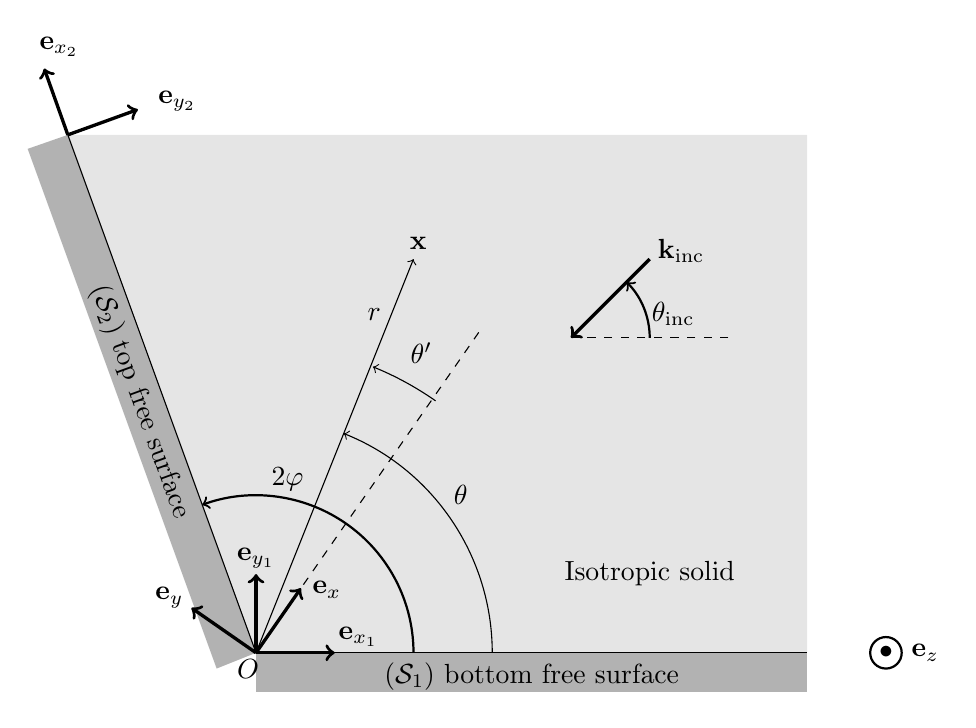
\begin{tikzpicture}
\fill[color=gray!20] (0,0) -- (7,0)  -- (7,6.5778) -- (-2.39,6.5778) -- cycle;  
\draw[ thick, ->] (2,0) arc (0:110:2);

\fill[color=gray!60] (0,0) -- (7,0)  -- (7,-0.5) -- (0,-0.5) -- cycle;  

\fill[color=gray!60] (0,0) --  (-2.39,6.5778) --(-2.9,6.4) -- (-0.5,-0.2) -- cycle; 

\draw[color = black]  (0,0) -- (7,0) node[midway,below] {($\mathcal{S}_1$) bottom free surface};

\draw[color = black]  (0,0) -- (-2.39,6.5778) node[midway,below,sloped] { ($\mathcal{S}_2$) top free surface};

\draw[very thick, ->] (-2.39,6.5778) -- (-2.69,7.42);

\node[scale=1] at (-2.5,7.7){ $\mathbf{e}_{x_2}$};

\draw[very thick, ->] (-2.39,6.5778) -- (-1.5,6.9);

\node at (-1,7){$\mathbf{e}_{y_2} $};


\node at (0.4,2.2){$2 \varphi$} ; 

\draw[very thick, ->] (0,0) -- (1,0);

\node at (1.3,0.2) {$\mathbf{e}_{x_1} $};

\draw[very thick, ->] (0,0) -- (0,1);

\node at (0,1.2){$\mathbf{e}_{y_1} $};

\node at (8,0) {$\bullet$};

\draw[thick] (8,0) circle (0.2);

\node at (8.5,0){$\mathbf{e}_{z}$};

\draw[very thick, ->] (0,0) -- (0.57,0.82);

\node at (0.9,0.8){$\mathbf{e}_x$};

\draw[very thick, ->] (0,0) -- (-0.82, 0.57);

\node at (-1.1,0.7){$\mathbf{e}_y$};

\draw[very thick, ->] (5,5) -- (4,4);

\draw[dashed] (6,4) -- (4,4);

\draw[ thick, ->] (5,4) arc (0:45:1);

\node at (5.3,4.3){$\theta_{\rm inc}$};

\node at (5.4,5.1){$\mathbf{k}_{\rm inc}$};

\node at (-0.1,-0.2){$O$};

\node at (5,1){Isotropic solid};

% point observation

\draw[->] (0,0) -- (2,5); 

\draw[->] (3,0) arc (0:68.2:3);

\draw[dashed] (0,0) -- (2.85,4.1);

\node at (2.6,2){$\theta$};

\node at (1.5,4.3){$r$};

\node at (2.06,5.2){$\mathbf{x}$};

\draw[->] (2.28,3.2) arc (55:68:4);

\node at (2.1,3.8){$\theta'$};

\end{tikzpicture}
\caption{Stress-free wedge of angle $2\varphi$ illuminated by a plane wave of wave vector $\mathbf{k}^{\rm inc}$. The dotted line is the wedge bisector.}
\label{C1:wedge}
\end{figure}

As seen in the previous section, an accurate uniform scattering model requires a trust-worthy initial \acrshort{gtd} solution in order to be developed. The aim of this thesis will therefore be to develop a generic and trust-worthy wedge diffraction \acrshort{gtd} model. To our knowledge, there is no fully analytical resolution of the problem of elastic wedge diffraction available in scientific literature, and the preferred approach is semi-analytical. We begin this work by a review of the two main existing 2D elastic wedge-diffraction models. These two models have been presented and compared by Gautesen and Fradkin \cite{GautesenFradkin}, who also discuss their numerical validation. Experimental validation  of these codes has been done by Chapman et al. \cite{ChapmanBurch}.

\subsection{Problem statement}
\label{C1:PbStatement}
The geometry of the problem is visible in Fig.~\ref{C1:wedge}. A stress-free wedge of angle $2\varphi<\pi$ is illuminated by a a plane wave which forms an angle $\theta_{inc}$ with the bottom face of the wedge. The problem is two-dimensional in the sense that the incident wave vector is in the plane normal to wedge edge. In all the following, the harmonic time-dependency factor $e^{- i\omega t}$ (where $\omega$ is the circular frequency and $t$ is time) will be omitted. $(0;\mathbf{e}_{x_1},\mathbf{e}_{y_1},\mathbf{e}_z)$ is the orthonormal basis of a Cartesian coordinate system where the $z$-axis coincides with the wedge edge and the $x_1$ axis coincides with the bottom face of the wedge. The polar coordinates associated to this system are $\mathbf{x}=(r,\theta)$. In this coordinate system, the incident wave vector is :
\begin{equation}
\mathbf{k}^{inc}=-(\cos\theta_{inc},\sin\theta_{inc})_{(\mathbf{e}_{x_1},\mathbf{e}_{y_1})}
\end{equation}
$(0;\mathbf{e}_x,\mathbf{e}_y,\mathbf{e}_z)$ is the orthonormal basis of a Cartesian coordinate system where the $x$-axis coincides with the wedge bisector and the polar coordinates associated to the system are $\mathbf{x}=(r,\theta')$.

In both of the following approaches, the the symmetry of the problem with respect to the wedge bisector is used and the problem is split in two : a symmetric problem (regarding the polarization of the incident wave) and an antisymmetric problem. This is done by introducing a wave vector symmetric to $\mathbf{k}^{inc}$ with respect to the bisector :
\begin{equation}
\mathbf{k}_{sym}=(-\cos\theta'_{inc},\sin\theta'_{inc})_{(\mathbf{e}_x,\mathbf{e}_y)}
\end{equation}
In the case of an incident L wave, the symmetric problem is constructed by considering that the incident wave is the sum of two plane waves of which the wave vectors are $\mathbf{k}^{inc}$ and $\mathbf{k}_{sym}$, see Fig.~\ref{Sym}. In this case, the polarization vectors $\mathbf{p}^{inc}=\mathbf{k}^{inc}$ and $\mathbf{p}_{sym}=\mathbf{k}_{sym}$ are symmetric. The antisymmetric problem is constructed by setting the incident wave to be the sum of two plane waves of which the wave vectors are $\mathbf{k}^{inc}$ and $-\mathbf{k}_{sym}$, see Fig.~\ref{Antisym}. In this case the polarization vectors $\mathbf{p}^{inc}$ and $-\mathbf{p}_{sym}$ are antisymmetric.

In the case of an incident T wave, the polarization vector is normal to the wave vector. Therefore, symmetric problem is constructed by setting $\mathbf{k}^{inc}$ and $-\mathbf{k}_{sym}$ as the incident wave vectors, see Fig.~\ref{Antisym} and the antisymmetric problem is constructed by setting $\mathbf{k}^{inc}$ and $\mathbf{k}_{sym}$ as the incident wave vectors, see Fig.~\ref{Sym}.

\begin{figure}[h]
    \centering
    \begin{subfigure}[b]{0.45\textwidth}
        \includegraphics[width=\textwidth]{images/chapter1/SymPb.png}
        \caption{Symmetric problem for an incident longitudinal wave or antisymmetric problem for an incident transversal wave}
        \label{Sym}
    \end{subfigure}
    ~ 
    \begin{subfigure}[b]{0.45\textwidth}
        \includegraphics[width=\textwidth]{images/chapter1/AntisymPb.png}
        \caption{Antisymmetric problem for an incident longitudinal wave or symmetric problem for an incident transversal wave}
        \label{Antisym}
    \end{subfigure}
    \caption{(Reproduced from \cite{AKDthese}) Symmetric and antisymmetric problems. Blue and red vectors are the wave vectors and green vectors are the polarization vectors of the transversal waves.}
    \label{SymAntisym}
\end{figure}

Both of the semi-analytic resolutions that will be described in the following deal with the symmetric and antisymmetric problems separately, in order to reduce the numerical part of the resolution by half. The first approach presented is called the \acrfull{si} method. The main steps of the resolution are presented but the technical details are not given.

\subsection{The \acrfull{si} Method}
The \acrfull{si} method was first proposed by Budaev \cite{BudaevBook,Budaev1,Budaev2} and Budaev and Bogy \cite{Rayleigh,Rayleigh2,Rayleigh3} have proposed the corresponding numerical scheme. The theory was completed and clarified by Kamotski et al. \cite{KamotskiFradkin}.

In this approach, the elastodynamic potentials $\psi_L$ and $\psi_T$ are the unknowns. They are related to the displacement field by :
\begin{equation}
\mathbf{u}=\mathbf{\nabla}\psi_L+\mathbf{\nabla}\times(\psi_T\mathbf{e}_z)
\label{C1:elastopotentials}
\end{equation}
where $\mathbf{\nabla}$ is the gradient operator and $\mathbf{\nabla}\times$ is the curl operator. These potentials satisfy the Helmoltz equations in the angular domain \cite{Achenbach} :
\begin{equation}
\Delta \psi_L+k_L^2\psi_L=0 \mbox{ and } \Delta \psi_T+k_T^2\psi_T=0 \rm \mbox{ for } |\theta'|<\varphi
\label{C1:Helmoltz}
\end{equation}
In addition, the wedge faces are stress-free, meaning :
\begin{equation}
\sigma_{r\theta'}=0 \mbox{ and } \sigma_{\theta'\theta'}=0 \mbox{ for } |\theta'|=\varphi
\label{C1:stresses}
\end{equation}
Sommerfeld \cite{Sommerfeld} has given an exact expression of these potentials in the form of an integral. This integral satisfies \eqref{C1:Helmoltz} as well as the radiation conditions at infinity \cite{SMtechnique} :
\begin{equation}
\psi_*(k_*r,\theta')=\int_{\gamma_++\gamma_-}e^{-ik_*r\cos\lambda}\Psi_*(\theta'+\lambda)\,d\lambda
\label{C1:Sommerfeld}
\end{equation}
where $*=L,T$,$\lambda$ is a complex angle, $\Psi_*$ are unknown amplitudes and contours $\gamma_+$ and $\gamma_-$ are represented on Fig.~\ref{C1:Somcontours}.

\begin{figure}
\centering
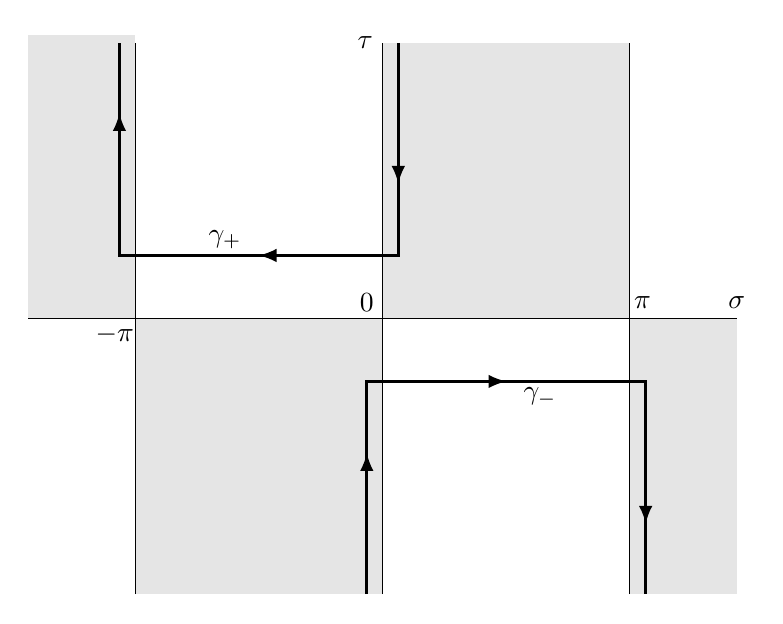
\begin{tikzpicture}
\fill[color=gray!20] (0,0) -- (0,3.5)  -- (pi,3.5) -- (pi,0);
\fill[color=gray!20] (-pi,-3.5) -- (0,-3.5)  -- (0,0) -- (-pi,0);
\fill[color=gray!20] (pi,-3.5) -- (4.5,-3.5)  -- (4.5,0) -- (pi,0);
\fill[color=gray!20] (-4.5,0) -- (-pi,0)  -- (-pi,3.6) -- (-4.5,3.6);
\draw[thin] (-4.5,0)  -- (4.5,0) node[above]{$\sigma$};
\draw[thin](0,-3.5)--(0,3.5) node[left]{$\tau$};
\draw[thin] (-pi,-3.5)  -- (-pi,3.5);
\draw[thin] (pi,-3.5)  -- (pi,3.5);
\node at (-3.4,-0.2) {$-\pi$};
\node at (3.3,0.2) {$\pi$};
\node at (-0.2,0.2) {$0$};
\node at (-2,1.0) {$\gamma_+$};
\node at (2,-1.0) {$\gamma_-$};

% segment de branche de coupure
%\draw[very thick] (-4, 0) -- (-2.2, 0);
%\draw[very thick] (4, 0) -- (2.2, 0);
%\draw (-4, 0) node {$\bullet$} ;
%\draw (-2.2, 0) node {$\bullet$} ;
%\draw (4, 0) node {$\bullet$} ;
%\draw (2.2, 0) node {$\bullet$} ;

% sommerfeld contour -pi
%\draw[black,very thick][domain=0:4.8] plot({-pi - acos(1/cosh(\x))*pi/180},\x);
%\draw[black,very thick][domain=-4.8:0] plot({-pi + acos(1/cosh(\x))*pi/180},\x);

% \draw[very thick,black,
%decoration={ markings,  % This schema allows for fine-tuning the positions of arrows 
%      mark=at position 0.1 with {\arrow{latex}}},
%      postaction={decorate}]
%      (-2.6404,-pi/6)  -- (-3.6428,pi/6); 

% sommerfeld contour pi
%\draw[black,very thick][domain=0:4.8] plot({pi - acos(1/cosh(\x))*pi/180},\x);
%\draw[black,very thick][domain=-4.8:0] plot({pi + acos(1/cosh(\x))*pi/180},\x);

% \draw[very thick,black,
%decoration={ markings,  % This schema allows for fine-tuning the positions of arrows 
%      mark=at position 0.1 with {\arrow{latex}}},
%      postaction={decorate}]
%     (2.6404,pi/6) -- (3.6428,-pi/6); 

% sommerfeld contour 0
%\draw[black,very thick, dashed][domain=0:4.8] plot({0 + acos(1/cosh(\x))*pi/180},\x);
%\draw[black,very thick, dashed][domain=-4.8:0] plot({0 - acos(1/cosh(\x))*pi/180},\x);

% \draw[thick,dashed,
%decoration={ markings,  % This schema allows for fine-tuning the positions of arrows 
%      mark=at position 0.1 with {\arrow{latex}}},
%      postaction={decorate}]
%      ( -0.5012,-pi/6)  -- (0.5012,pi/6); 

\draw[very thick,black,xshift=0pt,
decoration={ markings,  % This schema allows for fine-tuning the positions of arrows 
      mark=at position 0.2 with {\arrow{latex}},
      mark=at position 0.5 with {\arrow{latex}},
      mark=at position 0.9 with {\arrow{latex}}},
      postaction={decorate}]
      (0.2,3.5) -- (0.2,0.8) -- (-pi-0.2,0.8) -- (-pi -0.2,3.5); 
      
\draw[very thick,black,xshift=0pt,
decoration={ markings,  % This schema allows for fine-tuning the positions of arrows 
      mark=at position 0.2 with {\arrow{latex}},
      mark=at position 0.5 with {\arrow{latex}},
      mark=at position 0.9 with {\arrow{latex}}},
      postaction={decorate}]
      (-0.2,-3.5) -- (-0.2,-0.8) -- (pi+0.2,-0.8) -- (pi +0.2,-3.5);
\end{tikzpicture}
\caption{Sommerfeld contours of integration $\gamma_+$ and $\gamma_-$ in the complex plane $\lambda=\sigma+i\tau$.}
\label{C1:Somcontours}
\end{figure}

Following the decomposition of the problem, the unknown amplitudes can be decomposed into symmetric and antisymmetric amplitudes. The superscript $"+"$ refers to the symmetric problem and the superscript $"-"$ refers to the antisymmetric one. We then have :
\begin{equation}
\Psi_*(\lambda)=\Psi_*^+(\lambda)+\Psi_*^-(\lambda)
\end{equation}
where
\begin{subequations}
\begin{equation}
\Psi_L^\pm(\lambda)=\frac{1}{2}\lbrack\Psi_L(\lambda)\pm\Psi_L(-\lambda)\rbrack
\end{equation}
\begin{equation}
\Psi_T^\pm(\lambda)=\frac{1}{2}\lbrack\Psi_L(\lambda)\mp\Psi_L(-\lambda)\rbrack
\end{equation}
\end{subequations}
The symmetric and antisymmetric potentials $\psi_*^\pm$ associated to these amplitudes using \eqref{C1:Sommerfeld} are the solutions of the symmetric and antisymmetric problems. Kamotski et al. \cite{KamotskiFradkin} have shown that subsituting \eqref{C1:Sommerfeld} into \eqref{C1:stresses} yields the following system of functional equations :
\begin{multline}
\begin{pmatrix}
\Psi_L^\pm(g(\lambda)+\varphi)\\
\Psi_T^\pm(\lambda+\varphi)
\end{pmatrix}
=\pm\begin{pmatrix}
r_L^L(\lambda)&r_L^T(\lambda)\\
r_T^L(\lambda)&r_T^T(\lambda)
\end{pmatrix} 
\begin{pmatrix}
\Psi_L^\pm(g(\lambda)-\varphi)\\
\Psi_T^\pm(\lambda-\varphi)
\end{pmatrix} \\
+\kappa^2 c_1^\pm\dfrac{\sqrt{\kappa^{-2}-\cos^2\lambda}}{\mathcal{R}(\lambda)} \begin{pmatrix}
\cos 2\lambda-\tan\varphi\sin 2\lambda \\
\sin 2\lambda+\tan\varphi\dfrac{\sin\lambda\cos 2\lambda}{\sqrt{\kappa^{-2}-\cos^2\lambda}}
\end{pmatrix}
\label{C1:SIfunctional}
\end{multline}
where $\kappa=c_L/c_T$,
\begin{equation}
g(\lambda)=\arccos(\kappa\cos\lambda),
\end{equation}
the potential reflection coefficients $r_L^L,r_L^T,r_T^L$ and $r_T^T$ for the traction-free elastic half-space are known explicitly and are given in \cite{KamotskiFradkin}, function $\mathcal{R}$ is called the Rayleigh function :
\begin{equation}
\mathcal{R}(\lambda)=\cos^2 2\lambda+2\sqrt{\kappa^{-2}-\cos^2\lambda}\sin 2\lambda \cos\lambda
\label{C1:defRayleigh}
\end{equation}
and finally $c_1^\pm$ are unknown constants.

Representation \eqref{C1:Sommerfeld} gives the total elastodynamic potentials, including incident and reflected fields. It is well known that the poles of the Sommerfeld amplitudes $\Psi_*$ lead to the \acrshort{ge} field. The Sommerfeld amplitudes $\Psi_*^\pm$ can therefore be decomposed into two parts : a "singular part" $\Psi_*^{\pm \, sing}$, containing these poles and a "regular part" $\Psi_*^{\pm \, reg}$
\begin{equation}
\Psi_*^\pm=\Psi_*^{\pm \, sing}+\Psi_*^{\pm \, reg}
\label{C1:singreg}
\end{equation}
where $\Psi_*^{\pm \, reg}$ is regular in the strip 
\begin{equation}
\{ \lambda \in \mathbb{C},\, \pi/2-\varphi \leq \rm Re \lambda \leq \pi/2+\varphi \}
\end{equation}
and
\begin{equation}
\Psi_*^{\pm sing}(\lambda)=\sum_j \dfrac{res^\pm(\pm \lambda_*^j)}{2}\cot\left(\dfrac{\lambda\mp\lambda_*^j}{2}\right)
\end{equation}
$\pm\lambda_*^j$ are the poles of the Sommerfeld amplitudes $\Psi_*^{\pm sing}$ and  $res^\pm(\pm \lambda_*^j)$ are the corresponding residues. These poles and residues are determined analytically thanks to a recursive pole propagation algorithm, which is explained in great detail by Kamta-Djakou in \cite{AKDthese} and will not be reproduced here. Decomposition \eqref{C1:singreg} is then substituted into \eqref{C1:SIfunctional} and the resulting system is solved numerically, thanks to the scheme proposed by Kamotski et al. \cite{KamotskiFradkin}.

The diffracted elastodynamic potentials $\psi_{\beta}^{GTD} $ can be expressed in terms of the Sommerfeld amplitudes by evaluating integral \eqref{C1:Sommerfeld} asymptotically with the steepest descent method (see appendix \ref{PhaseStationnaire}) :
\begin{equation}
\psi_{\beta}^{GTD}=(k_{\beta} r,\theta')=i\sqrt{2i\pi}\lbrack \Psi_{\beta}(\theta'-\pi)-\Psi_{\beta}(\pi+\theta')\rbrack \dfrac{e^{ik_{\beta}r}}{\sqrt{k_{\beta}r}}
\end{equation}
Using \eqref{C1:elastopotentials}, the diffracted displacement field is given by :
\begin{equation}
\mathbf{u}^{diff(SI)}(r,\theta')=D_L^{SI}(\theta')\dfrac{e^{ik_Lr}}{\sqrt{k_Lr}}\mathbf{e}_{r'}+D_T^{SI}(\theta')\dfrac{e^{ik_Tr}}{\sqrt{k_Tr}}\mathbf{e}_{\theta'}
\end{equation}
where
\begin{equation}
D_{\beta}^{SI}(\theta')=-k_{\beta}\sqrt{2i\pi}\lbrack \Psi_{\beta}(\theta'-\pi)-\Psi_{\beta}(\pi+\theta')\rbrack
\end{equation}

To summarize, following the steps of Kamotski et al. \cite{KamotskiFradkin}, the \acrshort{gtd} diffraction coefficient of a stress-free wedge of angle $2\varphi<\pi$ can be computed. First, Sommerfeld's integral formulation of the elastodynamic potentials \eqref{C1:Sommerfeld} is used to determine two systems of functional equations \eqref{C1:SIfunctional} of which the symmetric and antisymmetric Sommerfeld amplitudes are solution. These systems are then solved by determining the poles and residues of the Sommerfeld amplitudes analytically and computing the remaining regular function numerically. Finally, the \acrshort{gtd} diffraction coefficient is deduced. 

An other semi-analytic resolution technique is called the \acrfull{lt} method and is presented in the following. Once again, the main steps of the resolution will be presented but the technical details are not given.

\subsection{The \acrfull{lt} Method}
\label{C1:lt}
The \acrfull{lt} method is due to Gautesen, who had developed it in the case of an incident Rayleigh wave \cite{GautesenRayleigh,GautesenRayleigh2,GautesenRayleigh0,GautesenRayleigh4,GautesenRayleigh3}, and in the case of an incident longitudinal wave on a right-angled wedge\cite{GautesenLwave}. It has been extended to the case of an L or T elastic wave incident on a wedge of angle $2\varphi<\pi$ by Gautesen and Fradkin \cite{GautesenFradkin}.

In this approach, the unknown quantity is the elastodynamic displacement $\mathbf{u}=(u_1,u_2)_{(\mathbf{e}_{x_1},\mathbf{e}_{y_1})}$. Gautesen \cite{GautesenRayleigh} has expressed the components of the displacement field in the entire space (not just inside the wedge) as a single-layer potential, analogously to Lax's electromagnetic extinction theorem \cite{Lax} :
\begin{multline}
H(2\varphi-\theta)u_p(\mathbf{x})=u_p^{inc}(\mathbf{x})-\sum_{i=1}^2\int_0^{+\infty}\Big[ G_{i2}^{(p)}(x_1-l,x_2)u_i(l,0) \\
 +\sum_{j=1}^2\sum_{m=1}^2\sigma_{jm}^{(p)}(x_1-l\cos 2\varphi,x_2-l\sin 2\varphi)e_{x_2}^{(j)}e_{y_2}^{(m)}u^{(i)}(l) \Big] \, dl
 \label{C1:extthm}
\end{multline}
where H is the Heaviside function ($H(x)=1$ for $x>0$ and $0$ elswhere) $(0;\mathbf{e}_{x_2},\mathbf{e}_{y_2}, \mathbf{e}_z)$ is an orthonormal basis, shown on Fig.~\ref{C1:wedge} where the $x_2$-axis coincides with the top free surface and where $\mathbf{e}_{y_2}$ is directed towards the inside of the wedge, $G^{(p)}$ is Green's stress tensor, defined in section \ref{sectKA} and
\begin{eqnarray}
u^{(i)}(l)=
\left\{
\begin{array}{cc}
\mathbf{u}(l\cos 2\varphi,l\sin 2\varphi).\mathbf{e}_{x_2} & \mbox{ for } i=1 \\
\mathbf{u}(l\cos 2\varphi,l\sin 2\varphi).\mathbf{e}_{y_2} & \mbox{ for } i=2
\end{array}
\right.
\end{eqnarray}
Equation \eqref{C1:extthm} is simplified by working in the region $x_2<0$ where, in the case $2\varphi<\pi$, the left-hand side of \eqref{C1:extthm} vanishes. The equation then contains four unknowns $(u_1,u_2)(l,0)$ and $(u^{(1)},u^{(2)})(l)$. In order to reduce the number of unknowns by half, the problem is once again symmetrized as described in subsection \ref{C1:PbStatement}. As in the previous section, the $"+"$ sign describes the symmetric problem and the $"-"$ sign describes the antisymmetric problem. We then have :
\begin{equation}
u^{(i)\pm}(l)=\pm u_i^\pm(l,0), \hspace{2em} i=1,2, \hspace{2em} l>0
\end{equation}
Equation \eqref{C1:PbStatement} is then reduced to :
\begin{multline}
u_p^{inc \pm}(\mathbf{x})=\sum_{i=1}^2\int_0^{+\infty}\Big[ G_{i2}^{(p)}(x_1-l,x_2)u_i^\pm(l,0)\\
\pm\sum_{j=1}^2\sum_{m=1}^2\sigma_{jm}^{(p)}(x_1-l\cos 2\varphi,x_2-l\sin 2\varphi)e_{x_2}^{(j)}e_{y_2}^{(m)}u_i^\pm(l,0) \Big] \, dl
\label{C1:extthmsym}
\end{multline}
The Laplace transform of the displacement field is defined by :
\begin{equation}
\hat{u}_i(\xi)=k_T\int_0^{+\infty}u_i^\pm(l,0)e^{ik_Tl\xi}\, dl
\label{C1:defLapl}
\end{equation}
In the Laplace domain, for the sake of simplicity, the superscript $\pm$ is omitted but implied. In order to separate the contributions of the longitudinal and transversal waves, the curl and divergence operators of equation \eqref{C1:extthmsym} are successively taken. The Laplace transform, defined by \eqref{C1:defLapl}, is then applied to the resulting system, yielding
\begin{equation}
A(\xi)\begin{pmatrix}
\hat{u}_1(\xi)\\
\hat{u}_2(\xi)
\end{pmatrix}
= \begin{pmatrix}
f_T(\xi)-\hat{U}_Ts(\xi)\\
f_L(\xi)-\hat{U}_L(\xi)
\end{pmatrix}
\label{C1:LTsyst}
\end{equation}
where $U_T=\mathbf{\nabla}\times\mathbf{u}^\pm$ and $U_L=\mathbf{\nabla}.\mathbf{u}^\pm$ and 
\begin{subequations}
\begin{equation}
\hat{U}_T(\xi)=\pm\lbrack -a(T_T)\hat{u}_1(T_T)+\overline{b}_T(\xi)\hat{u}_2(T_T) \rbrack
\end{equation}
\begin{equation}
\hat{U}_L(\xi)=\pm\lbrack \overline{b}_L(\xi)\hat{u}_1(T_L)+a(T_L)\hat{u}_2(T_L) \rbrack
\end{equation}
\label{C1:ULUT}
\end{subequations}
and
\begin{equation}
A(\xi)=\begin{pmatrix}
a(\xi)&-b_T(\xi)\\
b_L(\xi)&a(\xi)
\end{pmatrix}
\label{C1:matA}
\end{equation}
In equations \eqref{C1:ULUT} and \eqref{C1:matA}, we have, for $*=L,T$ :
\begin{subequations}
\begin{equation}
a(\xi)=\kappa_T-2\xi^2
\end{equation}
\begin{equation}
b_*(\xi)=2\xi\gamma_*(\xi)
\end{equation}
\begin{equation}
\overline{b}_*(\xi)=2T_*\eta_*
\end{equation}
\end{subequations}
where $\kappa_*=c_L/c_*$ and
\begin{subequations}
\begin{equation}
\gamma_*(\xi)=\sqrt{\kappa_*^2-\xi^2}
\end{equation}
\begin{equation}
T_*(\xi)=\xi\cos 2\varphi+\gamma_*(\xi)\sin 2\varphi
\end{equation}
\begin{equation}
\eta_*(\xi)=\xi\sin 2\varphi-\gamma_*(\xi)\sin 2\varphi
\end{equation}
\end{subequations}
and finally
\begin{eqnarray}
f_*(\xi)=\left\{
\begin{array}{cc}
\mp2\pi\kappa_*^2\lbrack \sin\theta_{inc}\delta(\xi-\kappa_*\cos\theta_{inc})\sin(2\varphi-\theta_{inc})\delta(\xi-\kappa_*\cos(2\varphi-\theta_{inc}))\rbrack & \mbox{if } *=\alpha \\
0&\mbox{else}
\end{array}
\right.
\label{C1:fstar}
\end{eqnarray}
where $\alpha$ is the type of the incident wave. Note that equations \eqref{C1:LTsyst} to \eqref{C1:fstar} actually describe two systems of functional equations : one for the symmetric problem and one for the antisymmetric problem.

As for the \acrshort{si} method, the solution $\hat{\mathbf{u}}$ can be decomposed into two parts : a singular part $\hat{\mathbf{u}}^{sing}$ containing the poles of $\hat{\mathbf{u}}$, which represent the \acrshort{ge} field and a regular part $\hat{\mathbf{u}}^{reg}$ :
\begin{equation}
\hat{\mathbf{u}}=\hat{\mathbf{u}}^{sing}+\hat{\mathbf{u}}^{reg}
\label{C1:LTsingreg}
\end{equation}
where $\hat{\mathbf{u}}^{reg}$ is regular in the whole complex plane except for the branch 
\begin{equation}
\{ \xi \in \mathbb{C}, \, \, \mbox{ Im} \xi=0, \, \, \mbox{ Re} \xi<-1 \}
\end{equation}
and, for $i=1,2$,
\begin{equation}
\hat{u}_i^{sing}=\sum_j \dfrac{res(\xi_i^j)}{\xi-\xi_i^j}
\end{equation}
where $\xi_i^j$ are the poles of $\hat{u}_i$ and $res(\xi_i^j)$ are the corresponding residues. These poles and residues are determined analytically thanks to a recursive pole propagation algorithm, which is detailed in \cite{AKDthese} and will not be reproduced here. Decomposition \eqref{C1:LTsingreg} is then substituted into \eqref{C1:LTsyst} and the resulting system is solved numerically using the scheme proposed by Gautesen and Fradkin \cite{GautesenFradkin}. Using a far-field approximation of the extinction theorem \eqref{C1:extthm}, Gautesen and Fradkin show that the diffracted field is given by :
\begin{equation}
H(2\varphi-\theta)\mathbf{u}^{diff(LT)}(r,\theta)=D_L^{LT}(\theta)\dfrac{e^{ik_Lr}}{\sqrt{k_Lr}}\mathbf{e}_{r}+D_T^{LT}(\theta)\dfrac{e^{ik_Tr}}{\sqrt{k_Tr}}\mathbf{e}_{\theta}
\end{equation}
where the diffraction coefficients of the symmetric and antisymmetric problems are :
\begin{subequations}
\begin{equation}
\begin{split}
D_L^{LT(\pm)}&=\sqrt{\frac{\pi}{2i}} \kappa_T^2 D_L^{LT(inc)\pm}+\sin(2\theta)\hat{u}_1(-\cos\theta)+(\kappa_T^2-2\cos^2\theta)\hat{u}_2(-\cos\theta) \\
& \mp \lbrack \sin(4\varphi-2\theta)\hat{u}_1(-\cos(2\varphi-\theta))+(\kappa_T^2-2\cos^2(2\varphi-\theta))\hat{u}_2(-\cos(2\varphi-\theta))\rbrack
\end{split}
\end{equation}
\begin{equation}
\begin{split}
D_T^{LT(\pm)}&=\sqrt{\frac{\pi}{2i}} \kappa_T^2 D_T^{LT(inc)\pm}+\kappa_T\lbrack\cos(2\theta)\hat{u}_1(-\kappa_T\cos\theta)+\sin(2\theta)\hat{u}_2(-\kappa_T\cos\theta)\rbrack \\
& \pm \lbrack \cos(4\varphi-2\theta)\hat{u}_1(-\kappa_T\cos(2\varphi-\theta))+\sin(4\varphi-2\theta)\hat{u}_2(-\kappa_T\cos(2\varphi-\theta))\rbrack
\end{split}
\end{equation}
\end{subequations}
where
\begin{equation}
D_{\beta}^{LT(inc)\pm}= \left\{
\begin{matrix}
\delta(\theta-\pi-\theta_{inc})\pm\delta(\theta-\pi-2\varphi+\theta_{inc}) & \rm if & \alpha=\beta \\
0 & \rm else
\end{matrix}
\right.
\end{equation}


A second method for computing the \acrshort{gtd} diffraction coefficient of a stress-free wedge of angle $2\varphi<\pi$ has been presented, following the steps of Gautesen and Fradkin \cite{GautesenFradkin}. First, the extinction theorem is used to determine an integral formulation of the elastodynamic displacement field in the entire domain. Using this formulation, two functional systems of equations are derived (one for the symmetric problem and one for the antisymmetric problem) of which the components of the Laplace transform of the displacement field are the solution. These two systems are solved separately by determining the poles and residues of the unknowns and computing the remaining regular functions numerically. Finally the \acrshort{gtd} diffraction coefficient is deduced.

The two semi-analytical models that have been presented here have been validated numerically \cite{GautesenFradkin} and experimentally \cite{ChapmanBurch}. They have been developed for stress-free wedges of angle $2\varphi<\pi$. Though they could probably be extended to wedges of angle higher than $\pi$, this has, to our knowledge, not been done yet in the general case of an L or T incident wave. Furthermore, these methods are valid for 2D configurations (when the incident wave vector is in the plane normal to the wedge edge). A third method, called the \acrfull{sf} method has been developed by Croisille and Lebeau \cite{CroisilleLebeau} in the case of an acoustic wave incident on an immersed solid wedge of angle lower than $\pi$ and has been used by Kamotski and Lebeau \cite{KamotskiLebeau} to prove existence and uniqueness of the solution to the problem of diffraction of an elastic wave by a wedge of arbitrary angle (lower or higher than $\pi$). However, the corresponding resolution scheme is not given. In this thesis, this method will be extended to the 2D cases of an acoustic wave or and elastic wave diffracted by a wedge of arbitrary angle and to the 3D case of an elastic wave diffracted by a wedge of arbitrary angle.

\section*{Conclusion}
In this first chapter, a brief summary of existing high frequency scattering models is given. The first model is the \acrfull{ge} model, which is faster than other numerical models (such as finite elements or finite differences) but only computes the incident and reflected field and does not account for diffraction. To correct this and account for diffraction by edges, the \acrfull{gtd} has been developed. Both of these models are non-uniform in the sense that the resulting scattered field is not spatially continuous and therefore is not physical. 

In order to produce a physically relevant scattered field, some uniform high-frequency models have been proposed. The \acrfull{ka} is spatially uniform but doesn't model diffraction accurately. In order to overcome the limitations of the \acrshort{gtd} and \acrshort{ka}, they are combined in an other uniform model, called the \acrfull{ptd}. It is spatially uniform and computes the diffracted wave accurately. However, it can be computationally expensive. A less costly uniform method is the \acrfull{uat}. Like \acrshort{ptd}, it is a uniform model and is accurate for both the \acrshort{ge} contribution to the scattered field and the edge-diffracted contribution to the scattered field. However, \acrshort{uat} requires tracing of fictitious rays, which makes it difficult to implement for complex geometries. Finally, the \acrfull{utd} is a spatially uniform model which has been validated numerically, is computationally cheap and is simple to implement.

Apart from the Kirchhoff approximation, all of these uniform models are corrections of the \acrshort{gtd} model. In order to correctly compute the edge diffracted field, a generic and trustworthy \acrshort{gtd} solution is then necessary. For the canonical problem of elastic wave diffraction by a stress-free wedge, the two main existing \acrshort{gtd} solutions are the \acrfull{si} method and the \acrfull{lt} method. For the moment, these methods have only been developed in 2D and for wedge angles lower than $\pi$. The objective of this thesis is to develop a semi-analytical resolution scheme, based on a third method called the \acrfull{sf} method, and to extend it to the case of a 3D incidence.
%
% Deuxième chapitre
\chapter[][Acoustic Case]{The spectral functions method for acoustic wave diffraction by a stress-free
wedge : theory and validation}
\label{chap-acoustic}


\section*{Introduction}
The canonical problem of an acoustic, electromagnetic or elastodynamic plane wave diffraction by a wedge with Neumann or Dirichlet boundary conditions is a complex mathematical problem which has been of great interest to researchers for over a century.

The mathematical theory of wedge diffraction was first introduced by Sommerfeld \cite{Sommerfeld}, who gave an analytical expression of the exact solution of the diffraction problem of a scalar plane wave as a contour integral \cite{SMtechnique}. Macdonald \cite{Macdo} has expressed the scalar solution as a series, using the variables separation technique. Sommerfeld \cite{Sommerfeld} gave an analytical formula of the \acrfull{gtd} diffraction coefficient for an arbitrary-angled wedge (with Neumann or Dirichlet boundary conditions) illuminated by a scalar plane wave. This wedge \acrshort{gtd} coefficient can be used for scalar wave diffraction both in electromagnetics \cite{Kouyoumjian} and in acoustics \cite{Bouche,Bo}.

These methods of computation have been proposed without proof of solvability for the wedge diffraction problem. Castro and Kapanadze \cite{Castro} have proven existence and uniqueness of the solution for acoustic and electromagnetic plane waves using a detailed Fredholm analysis. Kamotski and Lebeau \cite{KamotskiLebeau} have proven existence and uniqueness of the solution to the elastic plane wave diffraction  by a soft wedge (Dirichlet boundary) problem using the Spectral Functions method in which the diffracted wave is modeled thanks to these spectral functions. Their demonstration is valid for all wedge angles but they do not propose any method of computation of the solution. The Spectral Functions method was at first developed by Croisille and Lebeau \cite{CroisilleLebeau} who proposed a numerical algorithm in order to compute these functions for elastic wedges of angle lower than $\pi$ immersed in a fluid. In this chapter, wedges of any angle (even larger than $\pi$) are taken into account, and the outside medium is void. There is only one wave type to be considered and Dirichlet or Neumann boundary conditions are supposed, as opposed to the case studied by Croisille and Lebeau \cite{CroisilleLebeau} where three propagation modes coupled by the boundary conditions are considered, but only for wedge angles lower than $\pi$.

In the field of seismic diffraction, other approaches have been developed. The problem of acoustic diffraction in a system of wedge-shaped regions was studied by Klem-Musatov \cite{Klem-Musatov}. Using the Malyuzhinetz transform, this problem is reduced to a system of functional equations. However, this system is too complex to be solved in general cases. A successive approximations method is proposed in the particular case of a wedge-shaped separation between two media having the same acoustic wave velocity or  in the case where the medium containing the incident wave is a wedge of angle lower than $\pi$. In the very general case of acoustic wave propagation in a homogeneous or inhomogeneous medium delimited by an arbitrary-shaped boundary, a mathematical model has been rigorously presented by Aizenberg and Ayzenberg \cite{Aizenberg}, providing the analytical feasible fundamental solution for this problem. The notion of feasible fundamental solution is a generalization of Green's function for an unbounded medium. Ayzenberg \cite{Ayzenberg} shows how this general mathematical model can be numerically applied to the case of wedge diffraction. This method is applied in the case of a spherical source and it appears that parallel computation is necessary to obtain a short computation time, whereas the spectral functions method is applied here in the case of plane-wave diffraction and a simple architecture is sufficient to obtain results for a short computation time. 

The aim of this chapter is to develop and implement the methodology of Croisille and Lebeau \cite{CroisilleLebeau} in the two-dimensional (i.e. the incident wave vector lies in the plane normal to the edge) case of an acoustic wave diffracted by a soft wedge immersed in a fluid (Dirichlet boundary condition) and propose a numerical validation of the method for angles both smaller and larger than $\pi$.  The expansion to all wedge angles is obtained using Kamotski and Lebeau's \cite{KamotskiLebeau} idea of defining a new angular variable, $\widetilde{2\varphi}$, defined in equation \eqref{phitilde}, thanks to which the complete resolution and the computation of the solution are proposed and developed here for all wedge angles with a single method. Numerical validation will be achieved by comparing the GTD approximation of the diffraction coefficient obtained using the spectral functions method, with the analytical expression given in \cite{Bouche,Bo} of the GTD approximation of the exact solution. 

The outline of the chapter is the following: section \ref{Chapter5:problem}. presents the problem and the diffraction coefficients are expressed in terms of the spectral functions. The resolution of the problem is discussed in section \ref{Chapter5:resolution}. Finally, numerical results are given in section \ref{Chapter5:results}. and compared to the analytical Sommerfeld solution. 

\section{Problem statement}
\label{Chapter5:problem}

Let us consider a stress-free wedge of angle $\varphi$ immersed in a fluid $\Omega_f$ constituted of the junction of two faces $\mathcal{S}_1$ and $\mathcal{S}_2$ (see Fig.~\ref{chapter5:figure1}). The inward unit vectors normal to each of these faces are noted $n_1$ and $n_2$ respectively. The Cartesian coordinate system $(O; \mathbf{e}_{x_1}, \mathbf{e}_{y_1} )$ is linked to the face $\mathcal{S}_1$ of the wedge and $(O;  \mathbf{e}_{x_2}, \mathbf{e}_{y_2} )$ is linked to the face $\mathcal{S}_2$. These Cartesian coordinate systems  have the same origin located on the wedge edge which coincides with the $z$-axis. Let $\mathbf{x} = (x_1,y_1)_{ (\mathbf{e}_{x_1}, \mathbf{e}_{y_1}) } = (x_2,y_2)_{ (\mathbf{e}_{x_2}, \mathbf{e}_{y_2})}$ be a position vector $\mathbf{x} = (r,\theta)$ in a local basis of polar coordinates associated to the Cartesian coordinates $(x_1,y_1)$. The time convention used in this chapter is $\exp(i\omega t)$. The wedge is thus irradiated by a velocity potential plane wave in the form
\begin{align}
\label{Chapter5:incidence_wave}
g^{\rm inc}(\mathbf{x},t) = A \, e^{i(\omega t - \mathbf{k}^{\rm inc} \cdot \mathbf{x})}
\end{align}

where $A$ is the amplitude of the incident velocity potential, $\omega$ is the circular frequency, $t$ is time and 
\begin{align}
\mathbf{k}^{\rm inc} = k_0 (-\cos \theta_{\rm inc},-\sin \theta_{\rm inc})_{(\mathbf{e}_{x_1}, \mathbf{e}_{y_1})}
\end{align}
is the wave vector of the incident wave with $k_0 = \omega/c_0$ being the wave number and $c_0$ is the sound velocity in the fluid.  The velocity potential in the fluid $g$ satisfies the motion equation in the fluid medium $\Omega_f$ surrounding the wedge 
\begin{equation}
\label{Chapter5:WaveMotion}
\frac{\partial^2 g}{\partial t^2} - c_0^2 \, \triangle g = 0
\end{equation}
and the boundary condition on the wedges faces
\begin{equation}
\label{Chapter5:CL}
Bg\mid_{\mathcal{S}_j} = 0, \quad j=1,2,
\end{equation}
where the expression of operator B is given by \eqref{Chapter5:CLDir} for Dirichlet boundary conditions and by \eqref{Chapter5:CLNeu} for Neumann boundary conditoins :
\begin{subequations}
\begin{equation}
\label{Chapter5:CLDir}
Bg = g \quad \mbox{for Dirichlet boundary conditons}
\end{equation}
\begin{equation}
\label{Chapter5:CLNeu}
Bg = \frac{\partial g}{\partial n} \quad \mbox{for Neumann boundary conditons}
\end{equation}
\end{subequations}

This common notation makes it possible to treat both cases simultaneously in the following developments.

\begin{figure}[h]
\centering
	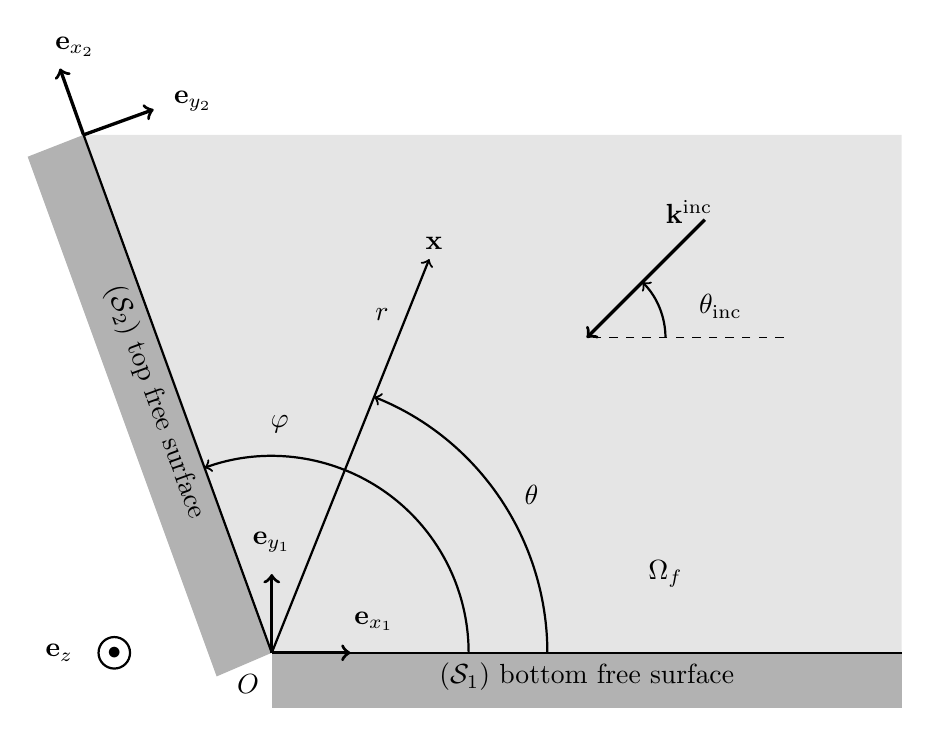
\begin{tikzpicture}
	\fill[color=gray!20] (0,0) -- (8,0)  -- (8,6.5778) -- (-2.39,6.5778) -- cycle;  
	\draw[ thick, ->] (2.5,0) arc (0:110:2.5);
	
	\fill[color=gray!60] (0,0) -- (8,0)  -- (8,-0.7) -- (0,-0.7) -- cycle;  
	
	\fill[color=gray!60] (0,0) --  (-2.39,6.5778) --(-3.1,6.3) -- (-0.7,-0.3) -- cycle; 
		
	\draw[thick, color = black]  (0,0) -- (8,0) node[midway,below] {($\mathcal{S}_1$) bottom free surface};
	
	\draw[thick, color = black]  (0,0) -- (-2.39,6.5778) node[midway,below,sloped] {($\mathcal{S}_2$) top free surface};
	
	\draw[very thick, ->] (-2.39,6.5778) -- (-2.69,7.42);
	
	\node[scale=1] at (-2.5,7.7){$\mathbf{e}_{x_2}$};
	
	\draw[very thick, ->] (-2.39,6.5778) -- (-1.5,6.9);
	
	\node at (-1,7){$\mathbf{e}_{y_2} $};
	
	
	\node at (0.1,2.9){$\varphi$} ; 
	
	\draw[very thick, ->] (0,0) -- (1,0);
	
	\node at (1.3,0.4) {$\mathbf{e}_{x_1} $};
	
	\draw[very thick, ->] (0,0) -- (0,1);
	
	\node at (0,1.4){$\mathbf{e}_{y_1} $};
	
	\node at (-2,-0.01) {$\bullet$};
	
	\draw[thick] (-2,0) circle (0.2);
	
	\node at (-2.7,0){$\mathbf{e}_{z}$};
	
	\draw[very thick, ->] (5.5,5.5) -- (4,4);
	
	\draw[dashed] (6.5,4) -- (4,4);
	
	\draw[thick, ->] (5,4) arc (0:45:1);
	
	\node at (5.7,4.4){$\theta_{\rm inc}$};
	
	\node at (5.3,5.6){ $\mathbf{k}^{\rm inc}$};
	
	\node at (-0.3,-0.4){ $O$};
	
	\node at (5,1){$\Omega_f$ };
	
	% point observation
	
	\draw[thick, ->] (0,0) -- (2,5); 
	
	\draw[thick, ->] (3.5,0) arc (0:68.2:3.5);
	
	\node at (3.3,2){$\theta$};
	
	\node at (1.4,4.3){$r$};
	
	\node at (2.06,5.2){$\mathbf{x}$};
	
	\end{tikzpicture}
	\caption
[Geometry of the problem]
{Stress-free wedge of angle $\varphi$ illuminated by a plane wave of wave vector $\mathbf{k}^{\rm inc}$.}
\label{chapter5:figure1}
\end{figure}
The dimensionless form of the problem is obtained  by defining the function $h$ by
\begin{equation}
\label{Chapter5:dimensionless}
g(\mathbf{x},t) = 2A \, e^{i \omega t} \, h(k_0 \mathbf{x}).  
\end{equation}

The dimensionless function $h$ is the sum of the  incident dimensionless  wave $h_{inc}$ and of the scattered dimensionless  wave $v$
\begin{equation}
h = h_{inc} + v
\label{decompinc}
\end{equation}
In this decomposition, the scattered wave $v$ is the sum of two fields : the Geometric-Elastodynamic (GE) field, which  is the sum of the possibly multiple specular reflections of the incident wave and of fictitious fields compensating the incident wave in shadow zones, and the diffracted field. A detailed description of the GE field, in the case of a half-plane scatterer, is given by Kamta-Djakou et al. \cite{Audrey}.

The system \eqref{Chapter5:WaveMotion}-\eqref{Chapter5:CL} is equivalent to the following  system of equations for the dimensionless problem, obtained by inserting Fourier transform \eqref{Chapter5:dimensionless} and decomposition \eqref{decompinc} into equations \eqref{Chapter5:WaveMotion} and \eqref{Chapter5:CL}
\begin{equation}
\label{Chapter5:Adimen_waveMotion}
\begin{cases}
(\triangle+1)v =  0 \quad \text{in } \Omega_f, \\
Bv =  -Bh_{inc} \quad \quad \quad \text{on } \mathcal{S}_j, \quad j=1,2
\end{cases}.
\end{equation}

In order to obtain a solution to this problem which is physically relevant, the limiting absorption principle is used. It consists in substituting the wave number $k_0$ by a complex one $k_0 e^{-i\epsilon} $ with $\epsilon > 0$. This means that absorption occurs in the medium and thus the scattered waves attenuate with the distance. The system (\ref{Chapter5:Adimen_waveMotion}) then becomes :
\begin{equation}
\label{Chapter5:waveMotion_epsilon}
(S_\epsilon^*) \quad
\begin{cases}
(\triangle+ \, e^{-2i\epsilon}) v^\epsilon  =  0 \quad \text{in } \Omega_f, \\
Bv^\epsilon  =  -Bh_{\rm inc}^\epsilon  \quad \text{on } \mathcal{S}_j, \quad j=1,2
\end{cases}
\end{equation}

The physically relevant solution to (\ref{Chapter5:Adimen_waveMotion}), called the outgoing solution, can now be defined. It is the one obtained when taking $\epsilon \to 0$ in (\ref{Chapter5:waveMotion_epsilon}). This limit is noted $v^0$. Its integral representation is found hereafter.

\subsection{Outgoing solution: integral representation}
\label{integral_representation}

First, a special class of distributions is defined.
\begin{definition}
The class of distributions $\mathcal{A}$ is defined as follows. The distribution $f\in \mathcal{A}$ if :
\begin{itemize}
\item $f \in \mathcal{L}^2(\mathbb{R})$ (f is a tempered distribution)
\item supp$(f) \subset \lbrack 0,+\infty \lbrack$
\item $\exists C_0>0$ such that
$$ \sup_{-\pi<\theta<0} \int_{\rho>C_0}|\hat{f}(\rho e^{i\theta})|^2\,d\rho <\infty$$
where $\hat{f}$ is the Fourier transform of $f$ defined by $\hat{f}(\xi)=\int_{\mathbb{R}}f(x)e^{-ix\xi}\, dx$.
\item $\hat{f}(\xi)$ is holomorphic near $\xi=1$
\end{itemize}
\label{defClassA}
\end{definition}
The outgoing solution to (\ref{Chapter5:Adimen_waveMotion}) can now be defined properly.

\begin{definition}
An outgoing solution of the equation (\ref{Chapter5:Adimen_waveMotion}) is a solution v of the form 
\begin{equation}
\label{Chapter5:decomposition}
v=v_1|_{\Omega_f}+v_2|_{\Omega_f}
\end{equation}
where, for $j=1,2$ :
\begin{equation}
\label{inv_potentiels}
v_j=-\lim_{\epsilon \to 0} \left(\Delta+e^{-2i\epsilon}\right)^{-1} \left[ \alpha_j \otimes \delta_{\mathcal{S}_j} \right]
\end{equation}
$\alpha_j \in \mathcal{A}$ are unknown and $\delta_{\mathcal{S}_1}$ and $\delta_{\mathcal{S}_2}$ are the Dirac delta functions on the faces $\mathcal{S}_1$ and $\mathcal{S}_2$ of the wedge respectively (these functions verify $\delta_{\mathcal{S}_j}(x,y)=1$ on $\mathcal{S}_j$, and $\delta_{\mathcal{S}_j}(x,y)=0$ elsewhere).

\end{definition}
The following theorem is proven by Croisille and Lebeau in \cite{CroisilleLebeau} :
\begin{theorem}
The equation \eqref{Chapter5:Adimen_waveMotion} admits a unique outgoing solution.
\end{theorem}

The aim of this chapter is to extend and detail the computation of this outgoing solution for the stress-free wedge immersed in a fluid using the spectral functions method.

The double Fourier transform of a tempered distribution and its inverse are defined by :
\begin{subequations}
\begin{equation}
\hat{f}(\xi,\eta)=\int \int_{\mathbb{R}^2}f(x,y)e^{-i(x\xi+y\eta)}\, {\rm d}x {\rm d}y
\label{fourierdef}
\end{equation}
\begin{equation}
f(x,y)=\frac{1}{4\pi^2}\int\int_{\mathbb{R}^2} \hat{f}(\xi,\eta)e^{i(x\xi+y\eta)}\rm d\xi \rm d\eta
\label{invfourierdef}
\end{equation}
\label{fullfourierdef}
\end{subequations}

The double Fourier transform of (\ref{inv_potentiels}) using \eqref{fourierdef} gives
\begin{equation}
\label{Fourier}
\hat{v_j^\epsilon} =  \left[ \xi^2 + \eta^2 - e^{-2i\epsilon} \right]^{-1} \hat{\alpha_j}.
\end{equation}

 The dimensionless velocity potential $v_j^\epsilon$ is then found by applying the inverse Fourier transform in $\xi$ and $\eta$ to \eqref{Fourier}. 
\begin{equation}
\label{velocity_inv_fourier2}
v_j^\epsilon = \dfrac{1}{4\pi^2}  \int_{-\infty}^{+\infty}\left( \int_{-\infty}^{+\infty} \dfrac{e^{iy_j\eta}}{ \xi^2 + \eta^2 - e^{-2i\epsilon}} {\rm d}\eta \right)\,  \hat{\alpha_j}(\xi) \,  e^{i x_j \xi}  {\rm d} \xi.
\end{equation}

For  $\epsilon \neq 0$, the inner integrand poles are given by
\begin{equation}
 \eta = \pm \sqrt{e^{-2i\epsilon} - \xi^2}  = \pm \zeta_0^\epsilon
\end{equation} 
and are never crossed by integration along the real axis. Integral \eqref{velocity_inv_fourier2} can be calculated using the residue theorem which leads to the following result
\begin{equation}
\label{champ_epsilon}
v_j^\epsilon(x_j,y_j) = \dfrac{i}{4\pi} \int_{-\infty}^{+\infty}  \dfrac{e^{i|y_j|\zeta_0^\epsilon(\xi)} e^{i x_j \xi}}{\zeta_0^\epsilon(\xi)} \hat{\alpha_j}(\xi) \, {\rm d}\xi.
\end{equation}
This integral is well defined if $\text{Im}(\zeta_0^\epsilon) > 0$, so that the exponential in the integral decreases with the distance $y_j$ and the absorption principle is respected. Function $\zeta_0^\epsilon(\xi)$ then satisfies for $\xi$ real
\begin{subequations}
\label{zeta_function}
\begin{align}
\zeta_0^\epsilon(\xi)&= i\sqrt{\xi^2-e^{-i\epsilon}} \quad \text{if} \quad \vert \xi\vert \geq 1,\\
\label{zeta_function_inferior1}
\zeta_0^\epsilon(\xi)&= -\sqrt{e^{-i\epsilon}-\xi^2} \quad  \text{if} \quad \vert \xi\vert \leq 1.
\end{align}
\end{subequations}
The branch points of the function $\zeta_0^\epsilon(\xi)$ are $\pm  \, e^{-i\epsilon}$. For $\epsilon > 0$, integral \eqref{champ_epsilon} is well defined because these complex singular points are never crossed by the integration contour (the real axis). The integration contour of \eqref{champ_epsilon}, is deformed into the contour $\Gamma_0$ illustrated on Fig.~\ref{chapter5:figure2} so that these singular points $\pm  \, e^{-i\epsilon}$ are not crossed by the new contour $\Gamma_0$  when $\epsilon \rightarrow 0$ (for which the physical outgoing solution of (\ref{Chapter5:waveMotion_epsilon}) is obtained). The curved arrows on Fig.~\ref{chapter5:figure2} are described later in section \ref{Chapter5:regular_part}.

Thus, even for $\epsilon=0$, the integral
\begin{equation}
\label{champ}
v_j^0(x_j,y_j) = \dfrac{i}{4\pi} \int_{\Gamma_0}  \dfrac{e^{i|y_j|\zeta_0^0(\xi)} e^{i x_j \xi}}{\zeta_0^0(\xi)} \hat{\alpha_j}(\xi)  \, {\rm d}\xi
\end{equation}
converges.
Using \eqref{Chapter5:decomposition}, our initial solution is then
\begin{equation}
\label{initial_sol}
v(\mathbf{x}) = v_1^0(x_1,y_1) + v_2^0(x_2,y_2)
\end{equation}

\begin{figure}[ht]%
	\centering
	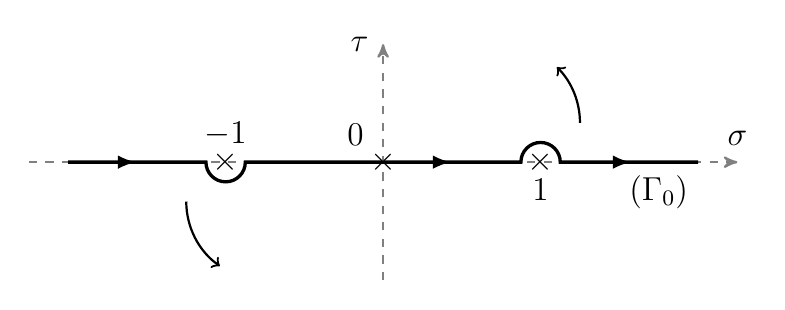
\begin{tikzpicture}
	\node at (0,0) {\large $\times$};
	\node at (-0.35,0.35) {\large $0$};
	\node at (2,0) {\large $\times$}; % Pole
	\node at (2,-0.35) {\large $1$};
	\node at (-2,0) {\large $\times$};
	\node at (-2,0.35) {\large $-1$}; %pole
	\node at (3.5,-0.38) {\large $(\Gamma_0)$};
	\draw[ thick, ->] (-2.5,-0.5) arc (180:235:1);
%	\node at (-2.8,-0.9) {\large $\mathcal{F}_1$};
	\draw[ thick, ->] (2.5,0.5) arc (0:45:1); %ici c'est les fleches 
	%\node at (2.8,0.9) {\large $\mathcal{F}_2$};
    \node at (4.5,0.3) {\large $\sigma$};
    \node at (-0.3,1.5) {\large $\tau$};
	\draw[step=1.5cm,gray,thick,dashed,->,>=stealth'] (-4.5,0) -- (4.5,0);
	\draw[step=1.5cm,gray,thick,dashed,->,>=stealth'] (0,-1.5) -- (0,1.5);
	\draw[very thick,black,yshift=0pt,
	decoration={ markings,  % This schema allows for fine-tuning the positions of arrows 
		mark=at position 0.1 with {\arrow{latex}},
		mark=at position 0.6 with {\arrow{latex}},
		mark=at position 0.9 with {\arrow{latex}}},
	postaction={decorate}]
	(-4,0)  -- (-2.25,0)  arc (-180:0:0.25)  -- (1.75,0)arc (180:0:0.25)  --  (4,0); % ca c'est l'axe
	\end{tikzpicture}
\caption
[Contour $\Gamma_0$]
{Integration contour $\Gamma_0$ in the complex plane $\xi = \sigma + i \tau$. The curved arrows show the deformation of $\Gamma_0$ into the imaginary axis.}
\label{chapter5:figure2}
\end{figure}

In the next section, an asymptotic evaluation of integral \eqref{champ} is conducted in order to obtain a far-field approximation of the diffracted wave. The \acrshort{gtd} diffraction coefficient is defined and its expression \eqref{GTDCoeff_SF} is given with respect to the spectral functions $\hat{\alpha}_1(\xi)$ and $\hat{\alpha}_2(\xi)$.
%One of the goals of this chapter is to compute the spectral functions $\hat{\alpha}_1(\xi)$ and $\hat{\alpha}_2(\xi)$ in order to find the GTD diffraction coefficient \eqref{GTDCoeff_SF}. 
%The accuracy of the spectral functions method is evaluated in section 4 by comparing results of \eqref{GTDCoeff_SF} with \eqref{GTDCoeff_Dir} in the case of Dirichlet boundary conditions and \eqref{GTDCoeff_Neu} in the case of Neumann boundary conditions. Section \ref{Chapter5:resolution} is devoted to the computation of the spectral functions $\hat{\alpha}_1$ and $\hat{\alpha}_2$.

\subsection{Far-field asymptotics}
\label{CoeffDiffAc}

Variable change $\xi = \cos \beta$, ${\rm d} \xi = - \sin \beta \, {\rm d}\beta$ allows us to transform \eqref{champ} for $j=1$ in
\begin{equation}
\label{face1_solution_exacte}
v_1^0(r \cos \theta,r \sin \theta) =  \dfrac{i}{4 \pi} \int_{C_0}  e^{i r (\cos \beta \cos \theta - |\sin \theta| \sin \beta)}  \hat{\alpha}_1( \cos \beta) \, {\rm d}\beta,
\end{equation}
where $C_0$ is depicted on Fig.~\ref{chapter5:figure3}. 

\begin{figure}[ht]%
\begin{center}
 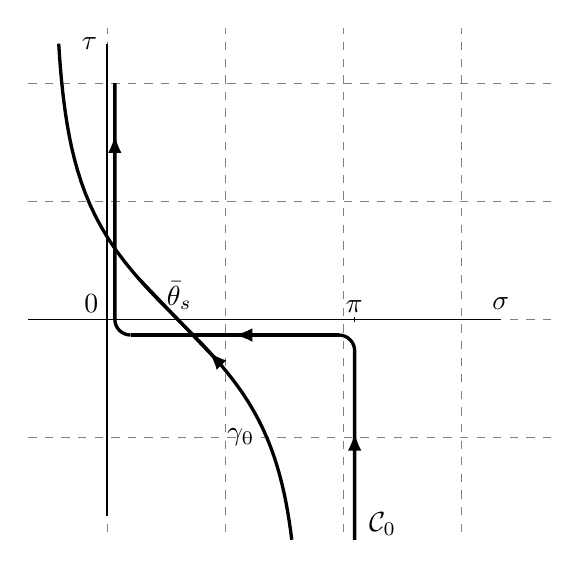
\begin{tikzpicture}
\draw[step=1.5cm,gray,very thin,dashed](-1,-2.7)grid(5.7,3.7);
%\draw[thin](-1,0)-- (0,0);
\draw[thin] (-1,0)  -- (5,0) node[above]{$\sigma$};
%\drawn[thin] -- (pi+1,0) node[below]{$\sigma$};
\draw[thin](0,-2.5)--(0,3.5) node[left]{$\tau$};
\foreach \x in {pi} {  
  \draw (\x,-1pt) -- (\x,1pt) node[pos=0,above] {$\pi$};
  }

\node at (-0.2,0.2) {$0$};
\node at (0.92,0.3) {$\bar{\theta}_s$};
%\node at (3.5,-3.8) {$(\mathcal{C}_\xi)$};
\node at (3.5,-2.6) {$\mathcal{C}_0$};
\node at (1.7,-1.5) {$\gamma_0$};

\draw[black,very thick][domain=0:3.5] plot({2*pi/7 - acos(1/cosh(\x))*pi/180},\x);
\draw[black,very thick][domain=-2.8:0] plot({2*pi/7 + acos(1/cosh(\x))*pi/180},\x);
\draw[very thick,black,xshift=0pt,
decoration={ markings,  % This schema allows for fine-tuning the positions of arrows 
      mark=at position 0.8 with {\arrow{latex}}},
      postaction={decorate}]
      (0.3,-0.2) arc (270:180:0.2) -- (0.1,3); 
\draw[very thick,black,yshift=0pt,
decoration={ markings,  % This schema allows for fine-tuning the positions of arrows 
      mark=at position 0.5 with {\arrow{latex}}},
      postaction={decorate}]
      (pi-0.2,-0.2) -- (0.3,-0.2) ;
%\draw[very thick] (0.3,0) arc (270:180:0.2);

\draw[very thick,black,xshift=89.5pt,
decoration={ markings,  % This schema allows for fine-tuning the positions of arrows 
      mark=at position 0.5 with {\arrow{latex}}},
      postaction={decorate}]
      (0,-2.8) -- (0,-0.4) arc (0:90:0.2) ;
      \draw[very thick,black,
decoration={ markings,  % This schema allows for fine-tuning the positions of arrows 
      mark=at position 0.1 with {\arrow{latex}}},
      postaction={decorate}]
      (1.3988,-pi/6)  -- (0.3964,pi/6);  
\end{tikzpicture}
\end{center}
\caption
[Integration path $\mathcal{C}_0$ and the steepest descent path $\gamma_0$ in the complex plane $\lambda = \sigma + i\tau$]
{Integration path $\mathcal{C}_0$ and the steepest descent path $\gamma_0$ in the complex plane $\lambda = \sigma + i\tau$. $\bar{\theta}_s$ is the phase stationary point.}
\label{chapter5:figure3}
\end{figure}


Let us introduce the variable $\bar{\theta}$ defined as
\begin{equation}
\label{obs}
\begin{cases}
\bar{\theta} = \theta \qquad \quad \; \text{if } \theta < \pi \\ 
\bar{\theta} = 2\pi - \theta \quad \text{if } \theta \geq \pi 
\end{cases}.
\end{equation}
Finally, using \eqref{obs} in \eqref{face1_solution_exacte}, we have
\begin{equation}
v_1^0(r \cos \theta,r \sin \theta) = \dfrac{i}{4 \pi} \int_{C_0}  e^{i r \cos ( \beta + \bar{\theta})} \hat{\alpha}_1(\cos \beta)  \, {\rm d}\beta.
\end{equation}
The same process is applied to \eqref{champ} for $j=2$ and leads to
\begin{equation}
v_2^0(r \cos (\varphi - \theta),r \sin (\varphi - \theta)) = \dfrac{i}{4 \pi} \int_{C_0}  e^{i r \cos ( \beta \, + \, \overline{\varphi - \theta})}  \hat{\alpha}_2( \cos \beta) \, {\rm d}\beta
\end{equation}
with $\overline{\varphi - \theta}$ defined in the same way as \eqref{obs}. The saddle points of the phase functions in these two equations are respectively $\beta = \bar{\theta}_s = \pi - \bar{\theta} $ and $\beta = \bar{\theta}_s = \pi - \overline{\varphi-\theta}$. These saddle points are always in the interval $[0,\pi]$. Poles of the spectral functions $\hat{\alpha}_1$ and $\hat{\alpha}_2$ may be crossed during the deformation of contour $C_0$ into the steepest descent path $\gamma_0$ (see Fig.~\ref{chapter5:figure3}). These poles and their corresponding residues are determined in section \ref{Chapter5:sing_part}. They contribute to the integrals \eqref{champ} and lead to the geometrical field, noted $v^{(GE)}$. Their contribution can be computed using the residue theorem. The resulting integral after the contour deformation is approximated using the steepest descent method (see appendix \ref{PhaseStationnaire}). The contribution of the saddle points $  \bar{\theta}_s $ are respectively:
\begin{equation}
\label{diffracted_field1}
v_1^{0 \rm (diff)}(x_1,y_1) = \dfrac{e^{-i\frac{\pi}{4}}}{2\sqrt{2\pi}}\dfrac{e^{-ir}}{\sqrt{r}} \hat{\alpha}_1( - \cos \theta)   
\end{equation}
and
\begin{equation}
\label{diffracted_field2}
v_2^{0 \rm (diff)}(x_2,y_2) = \dfrac{e^{-i\frac{\pi}{4}}}{2\sqrt{2\pi}} \dfrac{e^{-ir}}{\sqrt{r}} \hat{\alpha}_2( - \cos ( \varphi - \theta)).   
\end{equation}
Finally in the far-field approximation, $r \gg 1$, using \eqref{initial_sol} and \eqref{diffracted_field1} - \eqref{diffracted_field2}, the total field is 
\begin{equation}
v^{\rm tot} = v^{\rm (GE)} + v^{\rm diff}
\end{equation}
where $v^{diff}$ is the field diffracted by the wedge edge
\begin{equation}
\label{Chapter5:diff_field}
v^{ diff} = \dfrac{e^{-i\frac{\pi}{4}}}{2\sqrt{2\pi}} \dfrac{e^{-ir}}{\sqrt{r}} [\hat{\alpha}_1( - \cos \theta) + \hat{\alpha}_2( - \cos ( 2\varphi - \theta))].
\end{equation}
Using \eqref{Chapter5:dimensionless} and \eqref{Chapter5:diff_field}, the \acrshort{gtd} diffraction coefficient is defined as
\begin{equation}
\label{GTDCoeff_SF}
D^{GTD} = \dfrac{e^{-i\frac{\pi}{4}}}{\sqrt{2\pi}} \, [\hat{\alpha}_1( - \cos \theta) + \hat{\alpha}_2( - \cos ( 2\varphi - \theta))]
\end{equation}
where $\hat{\alpha}_1$ and $\hat{\alpha}_2$ are unknown spectral functions. 

One of the aims of this chapter is to compute the spectral functions $\hat{\alpha}_1(\xi)$ and $\hat{\alpha}_2(\xi)$ in order to find the \acrshort{gtd} diffraction coefficient \eqref{GTDCoeff_SF}. The accuracy of the spectral functions method is then evaluated by comparing results of \eqref{GTDCoeff_SF} with analytic expressions \eqref{GTDCoeff_Dir} in the case of Dirichlet boundaries and \eqref{GTDCoeff_Neu} in the case of Neumann boundaries. Section \ref{Chapter5:resolution} is devoted to the computation of the spectral functions $\hat{\alpha}_1$ and $\hat{\alpha}_2$.

\section{Spectral functions computation}
\label{Chapter5:resolution}

To compute the spectral functions, the functional equations satisfied by these spectral functions $\hat{\alpha}_1$ and $\hat{\alpha}_2$ first have to be determined.
\subsection{Functional equations of spectral functions}

The velocity potential in the boundary conditions of the system \eqref{Chapter5:waveMotion_epsilon} is substituted by its expression \eqref{initial_sol}. It then leads to the following system of equations for the boundary conditions on each wedge face:
\begin{equation}
\label{CL}
\begin{cases}
Bv_1^0(x_1,0) + Bv_2^0(x_2 \cos \varphi,x_2 \sin \varphi)  =  -Bv^0_{\rm inc} \mid_{\mathcal{S}_1}\\
Bv_1^0(x_1 \cos \varphi,x_1 \sin \varphi) + Bv_2^0(x_2,0)   =  -Bv^0_{\rm inc} \mid_{\mathcal{S}_2}
\end{cases}.
\end{equation}
The Fourier transform is applied to the potential velocity expression on the face of each wedge
\begin{align}
\mathcal{F}(x_j \mapsto v_j^0 (x_j,0))(\xi) & =  \dfrac{i}{4\pi} \int_{\Gamma_0}  \dfrac{\hat{\alpha_j}(\lambda)}{\zeta_0^0(\lambda)}  \left( \int_0^{\infty} \, e^{-i x_j (\xi-\lambda)} dx_j \right) {\rm d} \lambda,\\
& =  \dfrac{1}{4\pi} \int_{\Gamma_0} \dfrac{\hat{\alpha_j}(\lambda)}{\zeta_0^0(\lambda) (\xi - \lambda)} {\rm d} \lambda \nonumber
\end{align}
and
\begin{align}
\mathcal{F} \left( x_j \mapsto v_j^0 \left( x_j \cos \varphi,x_j \sin \varphi \right) \right)(\xi)  & =  \dfrac{i}{4\pi} \int_{\Gamma_0}  \dfrac{\hat{\alpha_j}(\lambda)}{\zeta_0^0(\lambda)}  \left( \int_0^{\infty} \, e^{-i x_j \left( \xi - \lambda  \, \cos \varphi - |\sin \varphi| \, \zeta_0^0(\lambda) \right)} dx_j \right) {\rm d} \lambda,\\
& = \dfrac{1}{4\pi} \int_{\Gamma_0} \dfrac{ \hat{\alpha_j}(\lambda)}{\zeta_0^0(\lambda) \left[ \xi - \lambda \, \cos \varphi  - |\sin \varphi| \, \zeta_0^0(\lambda) \right]} {\rm d} \lambda.  \nonumber
\end{align}
The potential velocity's normal derivative on the face of each wedge is computed using \eqref{champ}, and by noting that for each face $n_j=y_j$ (see Fig.~\ref{chapter5:figure1}) :
\begin{equation}
\frac{\partial v_j^0}{\partial n_j}(x_j,y_j) = -\frac{1}{4\pi} \int_{\Gamma_0} te^{i\xi x_j}e^{i|y_j|\zeta_0^0(\xi)} \hat{\alpha_j}(\xi)\, d\xi,
\end{equation}
where $t= \rm sgn \, y_j$. In order to go from one Cartesian coordinate system to another, the following change in variables is given for $j=1,2$ (see Fig.~\ref{chapter5:figure1}) :
\begin{eqnarray}
\label{changecoords}
\left\{
\begin{array}{l}
x_{3-j}=x_j\cos\varphi+y_j\sin\varphi \\
y_{3-j}=x_j\sin\varphi-y_j\cos\varphi
\end{array}
\right.
\end{eqnarray}
This yields :
\begin{align}
\frac{\partial v_j^0}{\partial n_{3-j}}&=\frac{\partial v_j^0}{\partial y_{3-j}}= \sin\varphi \frac{\partial v_j^0}{\partial x_j}-\cos\varphi \frac{\partial v_j^0}{\partial y_j}\\
&=-\frac{1}{4\pi}\int_{\Gamma_0}\frac{(\xi\sin\varphi-t\cos\varphi\zeta_0^0(\xi))}{\zeta_0^0(\xi)}e^{i(\xi x_j+|y_j|\zeta_0^0(\xi))}\hat{\alpha_j}(\xi)\,d\xi
\end{align}
The Fourier transform can now also be applied to the potential velocity's normal derivative on the each face of the wedge
\begin{align}
\mathcal{F}(x_j \mapsto \frac{\partial v_j^0}{\partial n_j} (x_j,0))(\xi)&=-\frac{1}{4\pi} \int_{\Gamma_0}  \hat{\alpha_j}(\lambda)\left( \int_0^{\infty} \, e^{-i x_j (\xi-\lambda)} dx_j \right)\, d \lambda \nonumber\\
&=\frac{i}{4\pi}\int_{\Gamma_0}\frac{\hat{\alpha_j}}{\xi-\lambda}\, d\lambda
\end{align}
and
\begin{align}
\mathcal{F} &\left( x_j \mapsto \frac{\partial v_j^0}{\partial n_{3-j}} ( x_j \cos \varphi,x_j \sin \varphi) \right)(\xi)  \nonumber\\
& =  -\frac{1}{4\pi} \int_{\Gamma_0}  \frac{(\lambda\sin\varphi-t\cos\varphi\zeta_0^0(\lambda))}{\zeta_0^0(\lambda)}\hat{\alpha_j}(\lambda)  \left( \int_0^{\infty} \, e^{-i x_j \left( \xi - \lambda  \, \cos \varphi - |\sin \varphi| \, \zeta_0^0(\lambda) \right)} dx_j \right) \,d \lambda, \nonumber\\
& = \frac{i}{4\pi} \int_{\Gamma_0} \dfrac{ \lbrack \lambda\sin\varphi-t\cos\varphi\zeta_0^0(\lambda)\rbrack \, \hat{\alpha_j}(\lambda)}{\zeta_0^0(\lambda) \left[ \xi - \lambda \, \cos \varphi  - |\sin \varphi| \, \zeta_0^0(\lambda) \right]} \, d\lambda,
\end{align}
here $t=\rm sgn \sin \varphi$.

The dimensionless incident wave on the faces $\mathcal{S}_1$ and $\mathcal{S}_2$ of the wedge which is involved at the right side of \eqref{CL} is respectively:
\begin{subequations}
\label{CL2}
\begin{align}
v^0_{\rm inc}(x_1,y_1) & =  \dfrac{1}{2} \, e^{i \, (x_1 \cos \theta_{inc}+y_1\sin\theta_{inc} ) } ,\\
v^0_{\rm inc}(x_2,y_2) & =   \dfrac{1}{2} \, e^{i \, (x_2 \cos (\varphi - \theta_{inc} )+y_2\sin(\varphi-\theta_{inc}))} 
\end{align}
\end{subequations}

Therefore, applying the Fourier transform to \eqref{CL} leads to the following functional system of equations:
\begin{equation}
\label{functional_eq}
\begin{cases}
DM(\hat{\alpha}_1)(\xi) + TM(\hat{\alpha}_2)(\xi) = \dfrac{W_1}{\xi - Z_1} \\
TM(\hat{\alpha}_1)(\xi) + DM(\hat{\alpha}_2)(\xi)  = \dfrac{W_2}{\xi - Z_2} 
\end{cases}
\end{equation}
where $Z_1 =  \cos \theta_{\rm inc}$, $Z_2 =  \cos (\varphi - \theta_{\rm inc})$, $W_1=W_2=1$ in the case of Dirichlet boundary conditions and $W_1=\sin\theta_{inc}, \quad W_2=\sin(\varphi-\theta_{inc})$ in the case of Neumann boundary conditions. $DM$ is an integral operator defined as
\begin{equation}
\label{DM_operator}
\begin{split}
DM(\hat{\alpha}_1)(\xi) = \int_{\Gamma_0} DM(\xi,\lambda) \, \hat{\alpha}_1(\lambda) \, d \lambda =\dfrac{1}{2i\pi} \int_{\Gamma_0} \dfrac{dm(\lambda)  }{\xi - \lambda} \hat{\alpha}_1(\lambda) \, d\lambda
\end{split}
\end{equation}
where 
\begin{equation}
\label{dmDir}
dm(\lambda) = \dfrac{1}{\zeta_0^0(\lambda)}
\end{equation}
in the case of Dirichlet boundary conditions and 
\begin{equation}
\label{dmNeu}
dm(\lambda)=1
\end{equation}
in the case of Neumann boundary conditions. 

$TM$ is an integral operator defined as
\begin{equation}
\label{TM_operator}
\begin{split}
TM(\hat{\alpha}_1)(\xi) &= \int_{\Gamma_0} TM(\xi,\lambda) \, \hat{\alpha}_1(\lambda) \, {\rm d} \lambda =\dfrac{1}{2i\pi} \int_{\Gamma_0} \dfrac{ tm(\lambda)}{ \xi- \lambda \cos \varphi  - |\sin \varphi| \zeta_0^0(\lambda)} \hat{\alpha}_1(\lambda) \, {\rm d} \lambda 
\end{split}
\end{equation}
where 
\begin{equation}
\label{tmDir}
tm(\lambda)=\dfrac{1}{\zeta_0^0(\lambda)}
\end{equation}
in the case of Dirichlet boundary conditions and 
\begin{equation}
\label{tmNeu}
tm(\lambda)=\dfrac{\lambda\sin\varphi-t\cos\varphi\zeta_0^0(\lambda)}{\zeta_0^0(\lambda)}
\end{equation}
in the case of Neumann boundary conditions.
Note that the function $TM$ can be expressed as
\begin{equation}
TM(\xi,\lambda) =  \dfrac{1}{2i\pi} \dfrac{ tm(\lambda)}{ \xi- T_0(\lambda)} , 
\end{equation}
where, applying the variable change $\lambda=\cos\theta$
\begin{equation}
\label{Trans_operator}
T_0(\lambda=\cos\theta) =  \lambda \cos \phiti  + \sin \phiti \, \zeta_0^0(\lambda) =  \cos (\theta + \phiti)
\end{equation}
with 
\begin{equation}
\phiti =
\begin{cases}
 \varphi \quad \text{if} \quad 0 < \varphi < \pi \qquad \\
 2\pi - \varphi \quad \text{if} \quad \pi < \varphi < 2\pi
 \label{phitilde}
\end{cases}
\end{equation}
Function $T_0$ is therefore called the translation operator, since it translates the complex angle $\theta$ to $\theta+\phiti$. By using this angular variable, defined differently for wedge angles lower and higher than $\pi$, the description of the spectral functions method can be written the same way for wedge angles lower and higher than $\pi$, even if the final results (the diffraction coefficients) are different for wedge angles $\pi<\varphi<2\pi$ and $2\pi-\varphi$. Indeed, the variable $\varphi$ appears in all the resolution, whereas the variable $\phiti$ appears only in the definition of the function $T_0$ in \eqref{Trans_operator} and of the domain $\Omega_0$ in which $T_0$ operates, defined as
\begin{equation}
\label{Domain_Omega0}
\Omega_0 =\{\xi\in\mathbb C, \ \xi=\cos \theta, \ 0< {\rm Re } \, \theta < \pi -\phiti \}.
\end{equation}
Domain $\Omega_0$ is delineated by the hyperbola 
\begin{equation}
\partial \Omega_0^+ = \{   \xi \in \mathbb{C}, \quad \xi = \cos \theta, \quad {\rm Re}  \theta = \pi - \phiti \}.
\end{equation}
Domain $\Omega_0$ and its upper boundary $\partial \Omega_0^+$ are illustrated on Fig.~\ref{chapter5:figure4}. Domain $\Omega_0$ is the grey area in Fig.~\ref{chapter5:figure4}.

\begin{figure}[h]
\centering
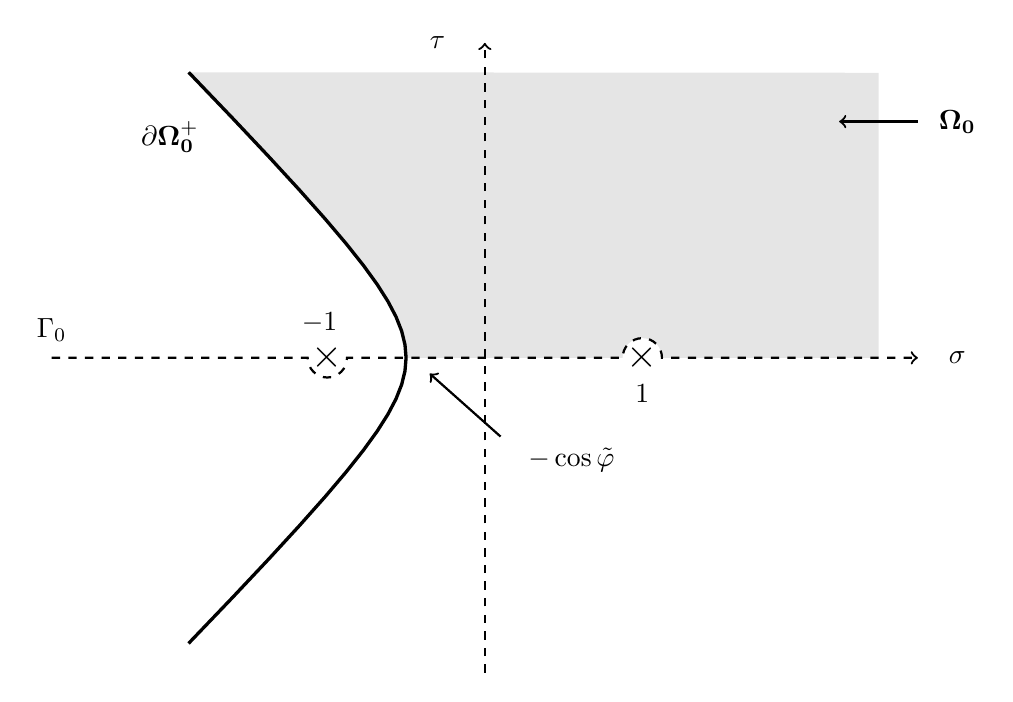
\begin{tikzpicture}
% Filling Omega_0
\fill [color=gray!20]
(5,0)
-- plot [domain=0:2] ({-cosh(\x)},{sinh(\x)})
-- (5,3.62)
-- cycle;

\fill[color=white] (2,0) circle (0.25);

\node at (2,0) {\Large $\mathbf{\times}$}; % Pole
\node at (2,-0.45) { $1$};
\node at (-2,0) {\Large $\mathbf{\times}$};
\node at (-2.1,0.45) {$-1$}; %pole
\node at (-5.5,0.35) {$\Gamma_0$};
\draw[dashed,thick, ->]
      (-5.5,0) -- (-2.25,0)  arc (-180:0:0.25)  -- (1.75,0)arc (180:0:0.25) -- (5.5,0);
\draw[dashed,thick,->]
	  (0,-4) -- (0,4);
\node at (6,0) {$\sigma$};
\node at (-0.6,4) { $\tau$};
      % axis

%% arrows indicating countour deformation
%\draw[ thick, ->] (-3,-0.25) arc (180:235:1);
%\node at (-3.2,-0.9) {$\mathcal{F}_1$};
%\draw[ thick, ->] (4.0,0.3) arc (0:45:1); 
%\node at (4.5,0.8) { $\mathcal{F}_2$};

% Hyperbola (contour  partial_Omega_0 )
\draw[black, very thick][domain=-2:2] plot({-cosh(\x)}, {sinh(\x)});
\node at (-4.0,2.8) { $\mathbf{\partial \Omega_0^+}$};
\draw[thick,->] (0.2,-1.0)--(-0.7,-0.2);
\node at (1.1,-1.3) {$-\cos \phiti$};

%  Omega_0
\draw [thick, ->] (5.5,3)--(4.5,3);
\node at (6,3) {$\mathbf{\Omega_0}$};

\end{tikzpicture}
\caption
[Contour $\partial \Omega_0^+$]
{Domain $\Omega_0$ (the grey area) and its upper boundary $\partial \Omega_0^+$. The lower boundary of $\Omega_0$ is the semi-axis $[-\cos \phiti,+\infty[$.}
\label{chapter5:figure4}
\end{figure}
Having found the system of functional equations, it is now resolved following the methodology of Croisille and Lebeau \cite{CroisilleLebeau}.

\subsection{System resolution}
\label{Chapter5:System_resolution}

The resolution of the system of functional equations \eqref{functional_eq} is necessary in order to find the values of the spectral functions $\hat{\alpha}_1 $ and $\hat{\alpha}_2 $. With these values, the diffraction coefficients can be computed using equation \eqref{GTDCoeff_SF}. 

It is shown in \cite{CroisilleLebeau} that $DM$ and $TM$ integral operators are constituted of a "singular term" and of a "regular term". For a singular function 
\begin{equation}
\label{Chapter5:arbitrary_function}
\phi(\xi) = \dfrac{1}{\xi - z},  \quad z \in \mathbb{C}\setminus ]-\infty,-1] \text{ with } {\rm Im} \, z \geqslant 0,
\end{equation}
$DM$ and $TM$ integral operators defined respectively in \eqref{DM_operator} and \eqref{TM_operator} can be decomposed using the residue theorem as
\begin{subequations}
\label{Int_op_decomp}
\begin{align}
\label{Int_op_decomp_DM}
DM(\phi)(\xi) &= \int_{\Gamma_0} DM(\xi,\lambda) \cdot \dfrac{1}{\lambda - z} \, d \lambda = \dfrac{dm(z)}{\xi - z}  + D_p(\xi,z) \\
\label{Int_op_decomp_TM}
TM(\phi)(\xi) &= \int_{\Gamma_0} TM(\xi,\lambda) \cdot \dfrac{1}{\lambda - z} \, d \lambda = \dfrac{tm(z) }{\xi - T_0(z)} 1_{\Omega_0}(z) + T_p(\xi,z),
\end{align}
\end{subequations}
where the function $T_0$ is defined in \eqref{Trans_operator} and where
\begin{equation}
1_{\Omega_0}(z) = 
\begin{cases}
1 \quad \text{if } z  \in \Omega_0, \\
0 \quad \text{else}
\end{cases}
\end{equation}
and integrals $D_p$ and $T_p$ are holomorphic on $\mathbb{C}\setminus ]-\infty,-1]$. Such integrals are expressed as
\begin{subequations}
\label{holomorphic_functions}
\begin{align}
\label{defDp}
D_p(\xi,z) &= \dfrac{1}{2\pi i}\int_{\Gamma_1} \dfrac{dm(\lambda)}{\xi-\lambda} \cdot \dfrac{1}{\lambda - z} d\lambda, \\
\label{defTp}
T_p(\xi,z) &= \dfrac{1}{2\pi i}\int_{\partial \Omega_0^+}  \dfrac{tm(\lambda)}{\xi-T_0(\lambda)} \cdot \dfrac{1}{\lambda - z} d\lambda.
\end{align}
\end{subequations}
Contours $\Gamma_1$ and $\partial \Omega_0^+$ are illustrated on Figs.~\ref{chapter5:figure5} and \ref{chapter5:figure4} respectively.

\begin{figure}[ht]
\centering
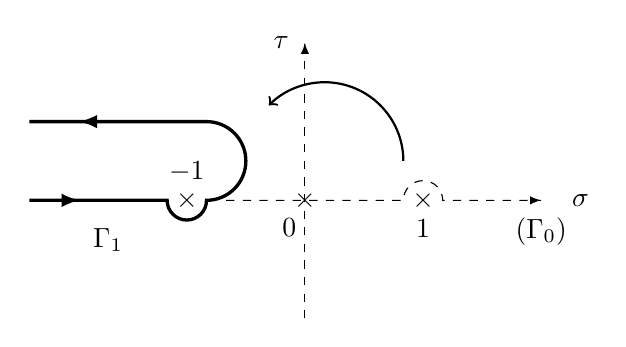
\begin{tikzpicture}
\node at (-0.5,0) {  $\times$};
\node at (-0.7,-0.35) { $0$};
\node at (1,0) { $\times$}; % Pole
\node at (1,-0.36) { $1$};

\node at (-2,0) { $\times$};
\node at (-2,0.36) {  $-1$}; %pole
\node at (-3,-0.5) { $\Gamma_1$};

\draw[dashed, decoration={markings,
 mark=at position 1.0 with {\arrow{latex}}},
      postaction={decorate}] (-1.5,0) -- (0.75,0) arc (180:0:0.25)-- (2.5,0);
\node at (3,0) {$\sigma$};
\draw[dashed, decoration={markings,
 mark=at position 1.0 with {\arrow{latex}}},
      postaction={decorate}] (-0.5,-1.5) -- (-0.5,2);
\node at (-0.8,2) {$\tau$};      

\node at (2.5,-0.4) {$(\Gamma_0)$};
      
\draw[ thick, ->] (0.75,0.5) arc (0:135:1); 
  

\draw[very thick, black, yshift=0pt,
decoration={ markings,  % This schema allows for fine-tuning the positions of arrows 
      mark=at position 0.1 with {\arrow{latex}},
      mark=at position 0.9 with {\arrow{latex}}},
      postaction={decorate}]
      (-4,0) -- (-2.25,0)  arc (-180:0:0.25) -- (-1.75,0) arc(-90:90:0.5)  -- (-4,1);
\end{tikzpicture}
\caption
[Contour $\Gamma_1$]
{Contour $\Gamma_1$. The curved arrow shows the deformation of $\Gamma_0$ (dashed line) into $\Gamma_1$.}
\label{chapter5:figure5}
\end{figure}

In the sequel, using the decomposition of the $DM$ and $TM$ operators for a function of the form of \eqref{Chapter5:arbitrary_function}, it will be shown that the unknown spectral functions $\hat{\alpha}_1$ and $\hat{\alpha}_2$ in the system \eqref{functional_eq} have a singular part. The first step for the resolution of the system \eqref{functional_eq} is then to determine this singular part.

\subsubsection{Singular part}
\label{Chapter5:sing_part}

It is well known that poles of the spectral functions lead to the reflections of the incident field on the wedge faces (these reflections can be multiple), and to the fictitious fields that compensate the incident wave in the shadow zones. The sum of these reflections with the fictitious compensating fields constitute the aforementioned GE field. The singular part of the spectral functions contains these poles. The goal of this subsection is to calculate the poles and the corresponding residues and then to determine the expression of the singular part of the spectral functions, by employing a recursive algorithm. 

Knowing the incident field on the wedge faces, the spectral function  $\hat{\alpha}_j$ can be written as
\begin{equation}
\label{Chapter5:ini_pol_propag}
\hat{\alpha}_j(\xi) = \dfrac{V_j}{\xi - Z_j} + X_j'(\xi), \quad j=1,2
\end{equation}
where $Z_1,Z_2$ are the initial poles, given in (\ref{functional_eq}) with unknown residues $V_1$ and $V_2$ and the functions $X_j'$ are unknown, $j=1,2$. From \eqref{Int_op_decomp_DM}, it is known that
\begin{equation}
\label{Chapter5:pole_propag_DM_1}
DM(\hat{\alpha}_j)(\xi) = \dfrac{dm(Z_j) \cdot V_j}{\xi - Z_j} + D_p(\xi,Z_j)\cdot V_j + DM( X_j')(\xi).
\end{equation}
By choosing $V_j =  dm^{-1}(Z_j).W_j$, the right hand side of the system \eqref{functional_eq} is suppressed by the first term in the right hand side of \eqref{Chapter5:pole_propag_DM_1}. The resulting system's unknown functions are $X'_j, \, j=1,2$ :
\begin{equation}
DM  (X_j' )(\xi)+ TM (X_{3-j}' )(\xi) = - TM  \left(  \dfrac{V_{3-j}}{\xi - Z_{3-j}} \right) (\xi)  - D_p(V_j,Z_j)(\xi) \qquad j=1,2
\end{equation}
Applying \eqref{Int_op_decomp_TM} yields
\begin{equation}
\label{Chapter5:pol_propag_step3}
TM  \left(  \dfrac{V_j}{\xi - Z_j} \right)(\xi) = \dfrac{tm(Z_j) \cdot V_j}{\xi - T_0(Z_j)}  \, 1_{\Omega_0}(Z_j) + T_p(\xi,Z_j)\cdot V_j \qquad j=1,2
\end{equation}
Thus, $X_j'$ has a pole at $\xi = Z_j^{1)} = T_0(Z_{3-j})$ if $Z_{3-j} \in \Omega_0$. The wave incident on face $\mathcal{S}_{3-j}$ is reflected. This reflected wave is incident on face $\mathcal{S}_j$, generating a new pole $Z_j^{(1)}=T_0(Z_{3-j})$. 
The unknown function $X_j'$ in \eqref{Chapter5:ini_pol_propag} is then decomposed as
\begin{equation}
\label{Chapter5:pol_propag_step2}
X_j'(\xi) =  \dfrac{V_j^{(1)}}{\xi - Z_j^{(1)}} + X_j''(\xi), \quad j=1,2
\end{equation}
where the function $ X_j''$ is unknown. 
Once again, the residues $V_j^{(1)}$ of these generated poles $Z_j^{(1)}$ are chosen so that they cancel the singular term in $DM(X_j')(\xi)$, found using formula \eqref{Int_op_decomp_DM}, compensating the singular term in the $TM$ operator in \eqref{Chapter5:pol_propag_step3}.

This pole propagation process is applied recursively in order to determine all the poles of the spectral functions $\hat{\alpha}_j$. This process stops when the generated poles are no longer in the domain $\Omega_0$ defined in \eqref{Domain_Omega0}. All the generated poles then belong to $\Omega_0$. 

At the end of this process, the spectral functions have the following decomposition
\begin{equation}
\label{spec_decomp}
\hat{\alpha}_j=Y_j+X_j, 
\end{equation}
where  $Y_j$ is the singular part, $X_j$ is the regular part  and $j=1,2$ is the face index. The singular part is expressed as
\begin{equation}
\label{sing_part}
 Y_j(\xi) = \sum_i {V_j^{(i)} \over \xi - Z_j^{(i)}},
\end{equation}
where $i \in \mathbb{N}$, $Z_j^{(0)} = Z_j$ defined in \eqref{functional_eq} is the initial pole on each face of the wedge, $V_j^{(0)}=V_j$ is the corresponding initial residue on each face of the wedge, 
\begin{equation}
\label{Generated_poles}
Z_j^{(i+1)} = T_0(Z_{3-j}^{(i)}) \quad j=1,2
\end{equation} 
are the different generated poles with their respective residues 
\begin{equation}
\label{Generated_residues}
V_j^{(i+1)}=-dm^{-1}(T_0(Z_{3-j}^{(i)})) \,  tm(Z_{3-j}^{(i)})) \, V_{3-j}^{(i)} \, 1_{\Omega_0}(Z_{3-j}^{(i)}), \quad  j=1,2.
\end{equation}
\paragraph{}
Figure \ref{poles} represents the generated poles in the complex plane for two different cases : figure \ref{poles80} for a wedge of angle $\varphi=80^o$ with an incident angle of $\theta_{inc}=55^o$ and figure \ref{poles20} for $\varphi=20^o$ and $\theta_{inc}=15^o$. As the wedge angle decreases, the number of poles increases, some poles being very close to one another, rendering the method less accurate for very small wedge angles.
\begin{figure}[h]
	\centering
	\begin{subfigure}[b]{0.4\textwidth}
	\begin{tikzpicture}[scale=2]
	\draw[->,>=stealth'] (-1.25,0) -- (1.25,0);
	\draw[->,>=stealth'] (0,-0.5) -- (0,0.5);
	\node at (1.25,0)[right]{Re};
	\node at (0,0.5)[right]{Im};
	
	\node at (-1,0){$\bullet$};
	\node at (1,0){$\bullet$};
	\draw (-1,0) node[below] {$-1$};
	\draw (1,0) node[below] {$1$};
	
	\node at ( 0.573576450    ,  0.00000000    ){$\times$};
	\node at ( 0.906307757    ,  0.00000000    ){$\times$};
	\node at (-0.258819222    ,  0.00000000    ){$\times$};
	\node at (-0.707106829    ,  0.00000000    ){$\times$};
	\end{tikzpicture}
	\subcaption{$\varphi=80^o, \, \theta_{inc}=55^o$}
    \label{poles80}
	\end{subfigure}
\hspace{1em}
\begin{subfigure}[b]{0.4\textwidth}
\begin{tikzpicture}[scale=2]
\draw[->,>=stealth'] (-1.25,0) -- (1.25,0);
\draw[->,>=stealth'] (0,-0.5) -- (0,0.5);
\node at (1.25,0)[right]{Re};
\node at (0,0.5)[right]{Im};

\node at ( 0.965925813    ,  0.00000000    ){$\times$};
\node at ( 0.996194720    ,  0.00000000    ){$\times$};
\node at ( 0.906307876    ,  0.00000000    ){$\times$};
\node at ( 0.819151998    ,  0.00000000    ){$\times$};
\node at ( 0.573576331    ,  0.00000000    ){$\times$};
\node at ( 0.707106948    ,  0.00000000    ){$\times$};
\node at ( 0.422618449    ,  0.00000000    ){$\times$};
\node at ( 0.258818895    ,  0.00000000    ){$\times$};
\node at ( -8.71558934E-02,  0.00000000    ){$\times$};
\node at (  8.71559381E-02,  0.00000000    ){$\times$};

\node at (-1,0){$\bullet$};
\node at (1,0){$\bullet$};
\draw (-1,0) node[below] {$-1$};
\draw (1,0) node[below] {$1$};
\end{tikzpicture}
\subcaption{$\varphi=20^o, \, \theta_{inc}=15^o$}
\label{poles20}
\end{subfigure}
\caption{Poles generated by the recursive algorithm plotted in the complex plane}
\label{poles}
\end{figure}

The second step of the system resolution is the determination of the regular part $X_j$ of the spectral function $\hat{\alpha}_j$, see Eq.~\eqref{spec_decomp}. The regular part is determined by using the Galerkin collocation method. Section \ref{Chapter5:regular_part} gives the principal steps of this resolution method. 

\subsubsection{Regular part}
\label{Chapter5:regular_part}

After the determination of the singular part of the solution using the pole propagation process explained in section \ref{Chapter5:sing_part}, the remaining system \ref{functional_eq} is by construction
\begin{equation}
\label{sys_regular}
\begin{cases}
DM(X_1)(\xi) + TM(X_2)(\xi) = -\underset{k}{\sum} \Big( D_p(\xi,Z_1^{(k)})\cdot V_1^{(k)}+ T_p(\xi,Z_2^{(k)})\cdot V_2^{(k)}\Big)\\
TM(X_1)(\xi) + DM(X_2)(\xi)  =  -\underset{k}{\sum} \Big( T_p(\xi,Z_1^{(k)})\cdot V_1^{(k)}+ D_p(\xi,Z_2^{(k)})\cdot V_2^{(k)}\Big)
\end{cases}
\end{equation}
where $X_j$, $j=1,2$ are the regular parts of the spectral functions \eqref{spec_decomp}, $D_p$ and $T_p$ functions are defined in \eqref{holomorphic_functions} and $Z_j^{(k)}$ are the poles of spectral function $\hat{\alpha}_j$  and their respective residues are $V_j^{(k)}$. According to Croisille and Lebeau \cite{CroisilleLebeau}, $D_p$ and $T_p$ are holomorphic on $\mathbb{C}\setminus  ]-\infty,-1]$ and therefore functions $X_1$ and $X_2$ are also holomorphic on this domain.

The functions $X_j(\xi)$, being holomorphic on $\mathbb{C}\setminus  ]-\infty,-1]$, can be approached in the vectorial subspace generated by $\varphi_k, \, 1 \leq k \leq N$ where
\begin{equation}
\label{Gal_basis}
\varphi_k(\xi) = \dfrac{d_k}{\xi + a_k}, \quad a_k \in [1,\infty[, \quad d_k=\sqrt{\frac{a_k}{\pi}}.
\end{equation}
The approximation of the solution $X_j(\xi)$ in this subspace of finite dimension is called a Galerkin approximation.

In the following, the integration contour $\Gamma_0$ pictured on Fig.~\ref{chapter5:figure2} is deformed into the imaginary axis. If $f(\lambda)$ is a holomorphic function on $\mathbb{C}\setminus  ]-\infty,-1]$, the function $\tilde f (y)=f(iy)$ is introduced so that $\tilde f$ is holomorphic on $\mathbb{C}\setminus i [1,\infty[ $. The variable change $\lambda = iy$ gives a new basis
\begin{equation}
\label{Galerkin_basis}
e_{a_k}(y) = \dfrac{d_k}{y-i{a_k}}=i\tilde \varphi(y), \quad \text{with} \quad d_k=\sqrt{\frac{a_k}{\pi}} \quad \text{and} \quad a_k \in [1,\infty[,
\end{equation}

Having an approximation basis of the regular part of the spectral functions, $X_j(\xi)$ can be expressed as
\begin{equation}
\label{regular_part_decomp}
X_j(\xi) \approx \sum_{k=1}^N \tilde{X}_j^k \, \varphi_k(\xi), \quad \tilde{X}_j^k \in \mathbb{C}.
\end{equation}
The coordinates $\tilde{X}_j^k$ are unknown. The system \eqref{sys_regular} then becomes, for $j=1,2$
\begin{equation}
\label{sys_regular_gal}
\sum_{k=1}^N \left[ \tilde{X}_j^k \, \int_{\Gamma_0} DM(\xi,\lambda) \varphi_k(\lambda) \, {\rm d} \lambda + \tilde{X}_{3-j}^k \, \int_{\Gamma_0} TM(\xi,\lambda) \varphi_k(\lambda) \, {\rm d} \lambda \right] = u_j(\xi), 
\end{equation}
where
\begin{equation}
\label{second_member}
u_j(\xi) = -\sum_k \Big( D_p(\xi,Z_j^k)\cdot V_j^k+ T_p(\xi,Z_{3-j}^k)\cdot V_{3-j}^k\Big) \qquad j=1,2
\end{equation}
The variable changes $\lambda = iy$ and $\xi = ix$ in \eqref{sys_regular_gal} lead to the following system $(j=1,2)$
\begin{equation}
\label{sys_regular_gal_def}
\sum_{k=1}^N \left[ \tilde{X}_j^k \, \int_{-\infty}^\infty  \widetilde{DM}(x,iy) \, e_{a_k}(y) {\rm d} y + \tilde{X}_{3-j}^k \, \int_{-\infty}^\infty  \widetilde{TM}(x,iy) \, e_{a_k}(y) {\rm d} y \right] = \tilde u_j(x) \\
\end{equation}
where $\widetilde{DM}(x,iy) = DM(ix,iy)$ and $\widetilde{TM}(x,iy) = TM(ix,iy)$. Following \cite{CroisilleLebeau}, we introduce another subspace of finite dimension in $L^2(\mathbb{R})$ which is generated by vectors $e_{b_k}$ with
\begin{equation}
\label{points_collocation}
e_{b_k}(y)=\frac{d_k}{y-ib_k}, \quad  \rm Re (b_k) \in [1,\infty[  \quad \text{and}  \quad {\rm Im} (b_k) = 0^-.
\end{equation}

Points $b_k$ are called collocation points.  The system \eqref{sys_regular_gal_def} is projected in this subspace using the following relation :
\begin{equation}
\label{dot_product}
\langle \tilde \phi\vert e_{b_k}\rangle_{L^2(\mathbb R)}= (-2i\pi) \, d_k \,  \phi (b_k)
\end{equation}

Using \eqref{dot_product}, the projection of the system \eqref{sys_regular_gal_def} leads to the following new system (for $j=1,2$)
\begin{equation}
\label{sys_regular_gal_col}
\begin{cases}
\sum_{k=1}^N \left[ \tilde{X}_j^k \, \int_{-\infty}^\infty DM(b_1,iy) e_{a_k}(y) \, {\rm d} y + \tilde{X}_{3-j}^k \, \int_{-\infty}^\infty TM(b_1,iy) e_{a_k}(y) \, {\rm d} y \right] = u_j(b_1) \\
 \qquad \qquad \qquad \qquad \qquad \qquad \qquad \qquad \vdots \\
\sum_{k=1}^N \left[ \tilde{X}_j^k \, \int_{-\infty}^\infty DM(b_N,iy) e_{a_k}(y) \, {\rm d} y + \tilde{X}_{3-j}^k \, \int_{-\infty}^\infty TM(b_N,iy) e_{a_k}(y) \, {\rm d} y \right] = u_j(b_N)
\end{cases}
\end{equation}
The obtained system \eqref{sys_regular_gal_col} is a linear system of equations and can be put in a matrix format:
\begin{equation}
\label{Syst_lineaire}
\begin{pmatrix}
\mathbb{D} & \mathbb{T}\\
\mathbb{T} & \mathbb{D}
\end{pmatrix}
\;
\begin{pmatrix}
\mathbb{X}_1\\
\mathbb{X}_2
\end{pmatrix}
 = 
\begin{pmatrix}
\mathbb{U}_1\\
\mathbb{U}_2
\end{pmatrix}
\end{equation}
where
\begin{equation}
\mathbb{X}_j = 
\begin{pmatrix}
\tilde{X}_j^1 \\
\vdots \\
\tilde{X}_j^N
\end{pmatrix}
\, \tilde{X}_j^k \in \mathbb{C}; \quad
\mathbb{U}_j = 
\begin{pmatrix}
u_j(b_1)\\
\vdots\\
u_j(b_N)\\
\end{pmatrix}
\, u_j(b_k) \in \mathbb{C}
\end{equation} 
and 
\begin{equation}
\label{D_matrix}
\mathbb{D}_{lk} = \int_{-\infty}^\infty DM(b_l,iy) e_{a_k}(y) \, {\rm d} y
\end{equation}
\begin{equation}
\label{T_matrix}
\mathbb{T}_{lk} = \int_{-\infty}^\infty TM(b_l,iy) e_{a_k}(y) \, {\rm d} y
\end{equation}
are the matrix elements of $\mathbb{D}$ and $\mathbb{T}$ respectively. System \eqref{Syst_lineaire} can be rewritten as
\begin{equation}
\label{Syst_lineaire_mod}
\begin{cases}
(\mathbb{D} + \mathbb{T}) \, (\mathbb{X}_1 + \mathbb{X}_2) = \mathbb{U}_1 +  \mathbb{U}_2\\
(\mathbb{D} - \mathbb{T}) \, (\mathbb{X}_1 - \mathbb{X}_2) = \mathbb{U}_1 - \mathbb{U}_2
\end{cases}.
\end{equation}
To approximate the regular part of the spectral functions \eqref{regular_part_decomp}, its coordinates $\tilde{X}_j^k$ in the Galerkin basis $\varphi_k, \, 1 \leq k \leq N$ defined in \eqref{Gal_basis} must be determined. These coordinates are the solutions of the linear system of equations \eqref{Syst_lineaire} or \eqref{Syst_lineaire_mod}. To resolve such a system, the matrices $\mathbb{D}$ and $\mathbb{T}$ and the right hand side $\mathbb{U}_{1,2}$ must be computed. 

\paragraph{Matrix calculation}

The first step is to determine $\mathbb{D}$ and $\mathbb{T}$ matrices.
Using \eqref{DM_operator} and \eqref{Galerkin_basis}, the $\mathbb{D}_{lk}$ elements defined in \eqref{D_matrix} can be expressed as
\begin{equation}
\label{matrice_D}
(-2i\pi) \mathbb{D}_{lk} =  -i d_k \mathcal{D}(a_k,b_l)
\end{equation}
with the function $\mathcal{D}(a,b)$ defined for $a>1$ and $b>1$ as
\begin{equation}
\label{ldbis}
\mathcal{D}(a,b) = \int_{-\infty}^{+\infty} \dfrac{dm(iy)}{y + ib} \, \dfrac{1}{y -ia} dy 
% = \int_{-\infty}^{+\infty} \dfrac{1}{y + ib} \, \dfrac{1}{y -ia} \, \dfrac{1}{\zeta_0^0(iy)} {\rm d}y. 
\end{equation}
This integral's value can be determined analytically. The details of the computation being a bit heavy, they are given in appendix \ref{finalDac}.

Using \eqref{TM_operator} and \eqref{Galerkin_basis} the $\mathbb{T}_{lk}$ elements defined in \eqref{T_matrix} can be expressed as
\begin{equation}
\label{matrice_T}
(-2i\pi) \mathbb{T}_{lk} =  - d_k \mathcal{T}(a_k,b_l)
\end{equation}
where the function $\mathcal{T}(a,b)$ is defined for $a>1$ and $b>1$ as
\begin{equation}
\label{ltbis}
\mathcal{T}(a,b) = \int_{-\infty}^{+\infty} \dfrac{tm(iy)}{ b - iy \cos 2\varphi  + |\sin 2\varphi| \sqrt{1+y^2}} \, \dfrac{1}{y -i a} \, dy . 
\end{equation}
This integral's value can be determined analytically. The details of the computation being a bit heavy, they are given in appendix \ref{finalTac}.

The matrices $\mathbb{D}$ and $\mathbb{T}$ are completely determined using \eqref{matrice_D} and \eqref{matrice_T} respectively. Their analytical properties are also known. In order to resolve the linear system of equations \eqref{Syst_lineaire} or \eqref{Syst_lineaire_mod},  their right hand side constituted of $\mathbb{U}_1$ and $\mathbb{U}_2$ must also be computed.

\paragraph{Determination of the right hand side of the system of equations}

Using \eqref{second_member}, the right hand side of the system \eqref{sys_regular_gal_col} which is calculated at the collocation points $b_l$ defined in \eqref{points_collocation}, $l \in \{ 1,2, \ldots, N \}$, is 
\begin{equation}
\label{second_member_new}
u_j(b_l) = -\sum_k \Big( D_p(b_l,Z_j^k)\cdot V_j^k+ T_p(b_l,Z_{3-j}^k)\cdot V_{3-j}^k\Big) \qquad j=1,2
\end{equation}
where $D_p$ and $T_p$ functions are defined in \eqref{Int_op_decomp} and $Z_j^k$ is defined in \eqref{Generated_poles}, $k \in \mathbb{N}^*$. 

Taking the definition of the $D_p$ function in \eqref{Int_op_decomp_DM}, and deforming the contour $\Gamma_0$ pictured on Fig.~\ref{chapter5:figure2} into the imaginary axis by applying the variable change $\lambda = iy$, we get
\begin{equation}
\label{Dp_final}
D_p(b_l,z) = {1\over 2\pi}\mathcal D(-z,b_l)-  {m(z)\over b_l-z}.
\end{equation}

Similarly, using the definition of the $T_p$ function given in \eqref{Int_op_decomp_TM}, and by deforming the integrand contour $\Gamma_0$ pictured on Fig.~\ref{chapter5:figure2} into the imaginary axis by applying the variable change $\lambda = iy$ we have
\begin{equation}
\label{Tp_final}
T_p(b_l,z) = 
\dfrac{1}{2i\pi} \mathcal T(-z,b_l) - \dfrac{m(z)}{b_l - T_0(z)} \mathbf{1} (z \in \Omega_0) .
\end{equation}

Expressions \eqref{Dp_final} of $D_p$ and \eqref{Tp_final} of $T_p$ functions are incorporated in the right hand side of the system \eqref{second_member_new} with $z = Z_j^k$ for each $u_j(b_l), \, j=1,2$. In this new expression, with the pole propagation process explained in section \ref{Chapter5:sing_part}, singular terms of $D_p$ and $T_p$ functions cancel each other. The remaining term in the right hand side of the system \eqref{second_member_new} is therefore, for $j=1,2; \quad l \in \{ 1,2, \ldots, N \}$
\begin{equation}
(2\pi i) \, u_j(b_l) =  - \sum_k \left( i \mathcal D(-Z_j^k,b_l)\cdot V_j^k  + \mathcal T(-Z_{3-j}^k,b_l) 
\cdot V_{3-j}^k  \right) +  \dfrac{2\pi i}{b_l - Z_j}
\end{equation}

Once all matrix terms have been calculated, system \eqref{Syst_lineaire} is resolved numerically using the numeric library Eigen for C++. With the resolution of this linear system of equations, the coordinates $\tilde{X}_j^k$ of the regular term $X_j$ of the spectral functions are known and therefore the regular term $X_j$ is approximated using \eqref{regular_part_decomp}. The spectral functions $\hat{\alpha}_j$ are then completely determined using \eqref{spec_decomp}, \eqref{sing_part} and \eqref{regular_part_decomp}. 

\subsection{Propagation of the solution}
\label{propag_sol}
The regular part approximation described previously is not accurate in the entire complex plane. There exists a procedure, called "propagation of the solution", which allows to propagate the accuracy of the regular part $X_j(\xi)$ of the spectral functions from $\xi \notin \Omega_0^-$, ${\rm Im} (\xi) <0$ where the approximation is valid to the domain $\Omega_0^-$ where it is not. The space $\Omega_0^-$ defined by
\begin{equation}
\label{defomegamoins}
\Omega_0^- = \{\xi \in \mathbb C, \ {\rm Im}(\xi) <0, \  \xi=\cos(\theta), \ \phiti < {\rm Re}(\theta)<\pi\}
\end{equation}
is represented in Fig.~\ref{chapter5:figure11}. 
The procedure consists in deriving new recursive equations by deforming the  contour $\Gamma_0$ in the integrals of the right-hand side of \eqref{sys_regular} into a new contour $\Gamma_2$ and taking into account the poles crossed in the process.

To begin, the contour $\Gamma_0$ in the $DM$ integral operator is deformed into contour $\Gamma_2$, visible Fig.~\ref{chapter5:figure8}. The half-space $\{ \lambda, {\rm Im} \ \lambda < 0 \}$ is then crossed during this contour deformation as shown by the curved arrow on Fig.~\ref{chapter5:figure8}.

\begin{figure}[ht]%
\centering
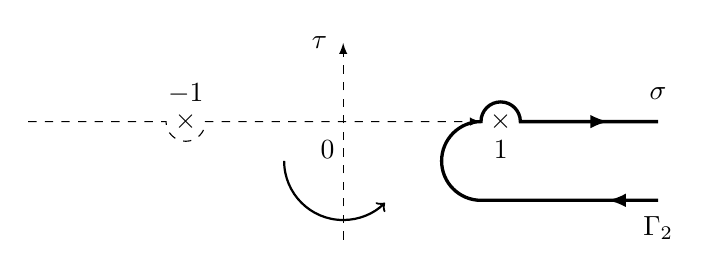
\begin{tikzpicture}
%\node at (-0.5,0) {  $\times$};
\node at (-0.2,-0.35) { $0$};
\node at (2,0) { $\times$}; % Pole
\node at (2,-0.36) { $1$};

\node at (-2,0) { $\times$};
\node at (-2,0.36) {  $-1$}; %pole
\node at (4,-1.35) { $\Gamma_2$};

\draw[dashed, decoration={markings,
 mark=at position 1.0 with {\arrow{latex}}},
      postaction={decorate}] (-4,0) -- (-2.25,0) arc (-180:0:0.25)-- (1.75,0);
      
\node at (4,0.35) {$\sigma$};

\draw[dashed, decoration={markings,
 mark=at position 1.0 with {\arrow{latex}}},
      postaction={decorate}] (0,-1.5) -- (0,1);
\node at (-0.3,1) {$\tau$};      

%\node at (2.5,-0.4) {$(\Gamma_0)$};
      
\draw[ thick, ->] (-0.75,-0.5) arc (0:135:-0.75); 
  

\draw[very thick, black, yshift=0pt,
decoration={ markings,  
      mark=at position 0.1 with {\arrow{latex}},
      mark=at position 0.9 with {\arrow{latex}}},
      postaction={decorate}]
      (4,-1) -- (1.75,-1)  arc (90:-90:-0.5) -- (1.75,0) arc(180:0:0.25)  -- (4,0);
\end{tikzpicture}
\caption
[Contour $\Gamma_2$]
{Contour $\Gamma_2$. The curved arrow shows the deformation of $\Gamma_0$ into $\Gamma_2$.}
\label{chapter5:figure8}
\end{figure}

During this contour deformation, only the poles
\begin{equation}
\lambda = \xi, \quad \text{with } {\rm Im}(\xi) <0 
\end{equation}
of the $DM$ function \eqref{DM_operator} are crossed and therefore, applying the residue theorem, we have for $\xi \in \mathbb{C}$, ${\rm Im}(\xi) <0$, $j=1,2$, 
\begin{equation}
\label{DM_propag_sol}
DM(X_j)(\xi) = \int_{\Gamma_0} DM(\xi,\lambda) X_j(\lambda) \, d \lambda  = \int_{\Gamma_2} DM(\xi,\lambda) X_j(\lambda) \, d \lambda + dm(\xi) X_j(\xi).
\end{equation}

The poles of the $TM$ function \eqref{TM_operator} are
$$ \lambda = T_0^{-1}(\xi) = \xi \, \cos \phiti  - \sin \phiti \, \zeta_0(\xi) = \cos (\theta - \phiti) \quad \text{if} \quad \xi = \cos \theta $$
$T_0^{-1}$ operates in the domain $\Omega_0^-$, therefore these poles are crossed during this contour deformation if and only if $\xi \in \Omega_0^-$ (see dotted area on Fig.~\ref{chapter5:figure11}).
The domain $\Omega_0^-$ is delineated by the hyperbola 
\begin{equation}
\partial \Omega_0^- = \{   \xi \in \mathbb{C}, \ {\rm Im}(\xi) <0,  \xi = \cos \theta, {\rm Re} \, \theta = \phiti \}.
\end{equation}
Domain $\Omega_0^-$ and contour $\partial \Omega_0^-$ are illustrated on Fig.~\ref{chapter5:figure11}.   

Applying the residue theorem to the $TM$ integral operator then gives for $\xi \in \mathbb{C}$, ${\rm Im}(\xi) <0$, $j=1,2$,
\begin{equation}
\label{TM_propag_sol}
\int_{\Gamma_0} TM(\xi,\zeta)X_j(\zeta)\, d\zeta = \int_{\Gamma_2}  TM(\xi,\zeta)X_j(\zeta)\, d\zeta+M_0(\xi).X_j(T^{-1}_0(\xi)),
\end{equation}
where the transfer operator $M_0$ is defined as :
\begin{equation}
\label{defM0}
M_0(\xi=\cos\theta)=-\frac{\sin(\theta-\tilde{\varphi})}{\sin\theta} tm(T_0^{-1}(\xi))1_{\Omega_0^-}(\xi)
\end{equation}

\begin{figure}[ht]%
\begin{center}
	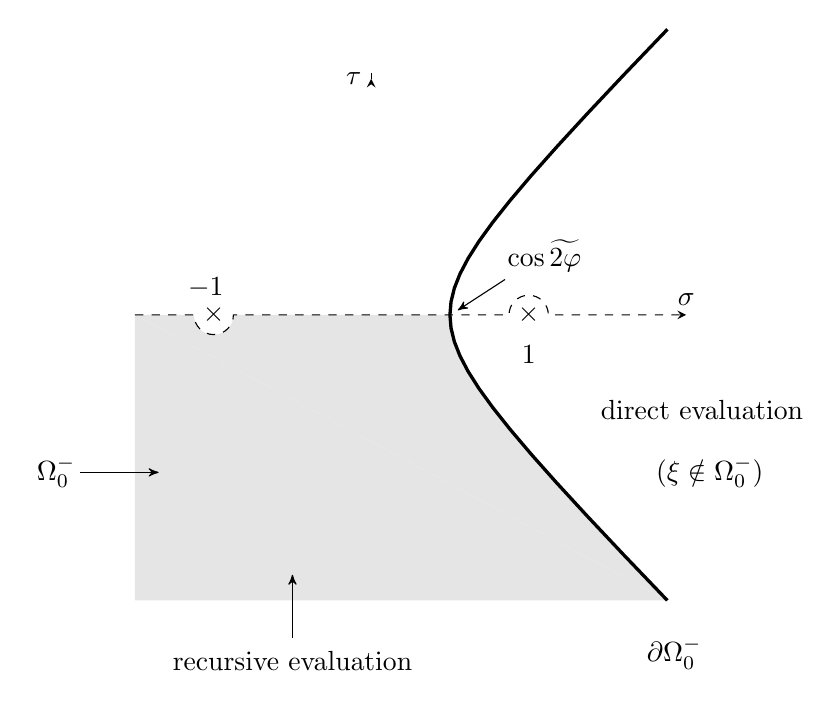
\begin{tikzpicture}
		% Filling Omega_0^-
	\fill [color=gray!20]
	(-1,0)
	-- plot [domain= 0:2] ({cosh(\x)},{-sinh(\x)})
	-- (-3,0)
	-- cycle;
	
	\fill [color=gray!20]
	({cosh(2)},{-sinh(2)})
	-- plot [domain= 0:-3] ({\x},{-sinh(2)})
	-- (-3,0)
	-- cycle;
	
	\fill[color=white] (-2,0) circle (0.25);
	
	\draw[dashed, ->,>=stealth] (-3,0)  -- (-2.25,0) arc(-180:0:0.25)--(1.75,0) arc (180:0:0.25)--(4,0) node[above]{$\sigma$};
	\draw[dashed, ->,>=stealth](0,3)--(0,3) node[left]{$\tau$};
	
	\node at (2,0) {$\times$}; % Pole
	\node at (2,-0.5) {$1$};
	\node at (-2,0) { $\times$};
	\node at (-2.1,0.35) {$-1$}; %pole
	
	% Hyperbola (contour  partial_Omega_0 )
	\draw[black, very thick][domain=-2:2] plot({cosh(\x)}, {-sinh(\x)});
	\node at (3.85,-4.3) {$\partial \Omega_0^-$};
	\draw[thin, ->,>=stealth'](1.7,0.45) -- (1.1, 0.06);
	\node at (2.2, 0.75) {$\cos \widetilde{2\varphi}$};
	
	% Omega_0
	\node at (-4,-2) {$\Omega_0^-$};
	\draw[->,>=stealth'] (-3.7, -2) -- (-2.7,-2);
	\draw[->,>=stealth'] (-1,-4.1) -- (-1,-3.3);
	\node at (-1,-4.4) {recursive evaluation};
	\node at (4.2,-1.2) { direct evaluation};
    \node at (4.3,-2) { $(\xi \notin \Omega_0^-)$};
	
	\end{tikzpicture}
\end{center}
\caption
[Domain $\Omega_0^-$ and its lower boundary $\partial \Omega_0^-$]
{Domain $\Omega_0^-$ and its lower boundary $\partial \Omega_0^-$ in the complex plane $\xi=\sigma + i \tau$. $\Omega_0^-$ is delimited by $\partial \Omega_0^-$ andthe semi-axis $]-\infty, \cos \widetilde{2\varphi}]$. }
\label{chapter5:figure11}
\end{figure}


Using \eqref{DM_propag_sol} and \eqref{TM_propag_sol} in the system of functional equations \eqref{sys_regular}, a new equivalent system is obtained for $\xi \in \mathbb{C}$, ${\rm Im}(\xi) <0$:
\begin{equation}
\label{propag_sol_sys}
\begin{cases}
X_1(\xi) = g_1(\xi) -  dm^{-1}(\xi)M_0(\xi)X_2(T_0^{-1}(\xi)) \\
\\
X_2(\xi) = g_2(\xi) - dm^{-1}(\xi)M_0(\xi)X_1(T_0^{-1}(\xi))
\end{cases}
\end{equation}
where
\begin{equation}
g_j(\xi) = dm(\xi)^{-1} \left[ u_j(\xi) - \int_{\Gamma_2} DM(\xi,\lambda) \, X_j(\lambda) \, {\rm d} \lambda - \int_{\Gamma_2} TM(\xi,\lambda) \, X_{3-j}(\lambda) \, {\rm d} \lambda \right] \\
\end{equation}
Formula \eqref{propag_sol_sys} is called the recursive formula because it uses the value of the regular function $X_2$ at point $T_0^{-1}(\xi)$ to compute the value of $X_1$ at the point $\xi$ where the approximation is not valid (and vice-versa). If the translation from $\xi$ to $T_0^{-1}(\xi)$ is not sufficient to reach the domain $\mathbb{C} \backslash \Omega_0^-$ where the approximation is valid, then the use of the formula is repeated as many times as necessary (computing $X_2(T_0^{-1}(\xi))$ using the value of $X_1(T_0^{-2}(\xi))$, etc.). This recursive evaluation can be summed up in one concise formula, for $j=1,2$ :
\begin{equation}
X_j(\xi)= \sum_{k} R^{(k)}\mathcal{G}_j^{(k)}(\xi^{(k)}),
\label{prop_concise_ac}
\end{equation}
where $k \in \mathbb{N}$, $\xi^{(0)}=\xi$ is the initial point at which function $X_j$ is evaluated and $R^{(0)}=1$. The computation points $\xi^{(k)}$ and the coefficients $R^{(k)}$ are determined recursively :
\begin{equation}
\xi^{(k+1)}=T_0^{-1}(\xi^{(k)}) \quad \rm if \quad \xi^{(k)} \in \Omega_0^-
\end{equation}
are the generated evaluation points with the corresponding coefficients 
\begin{equation}
R^{(k+1)}=-R^{(k)}.dm^{-1}(\xi^{(k)}).M_0(\xi^{(k)})
\end{equation}
The term $1_{\Omega_0^-}$ appears in the expression \eqref{defM0} of the transfer operator $M_0$, ensuring that the process stops when the generated evaluation points are no longer in $\Omega_0^-$. Finally, the operator $\mathcal{G}_j^{(k)}$ is defined in the following manner :
\begin{eqnarray}
\mathcal{G}_j(\xi^{(k)})=
\left\{
\begin{array}{l}
g_j(\xi^{(k)}) \mbox{ if }k \mbox{ is even } \\
g_{3-j}(\xi^{(k)}) \mbox{ if }k \mbox{ is odd}\\
\end{array}
\right.
\end{eqnarray}
In practice, formulation \eqref{prop_concise_ac} is implemented to evaluate the regular part of the system numerically. In order to do so, the points $\xi^{(k)}$  and the corresponding coefficients $R^{(k)}$ are determined recursively, using an algorithm similar to the one used to determine the poles and residues of the spectral functions. To calculate $g_j$ functions, we need to compute
\begin{equation*}
\int_{\Gamma_2} DM(\xi,\lambda) \, X_j(\lambda) {\rm d} \lambda \approx \sum_k \tilde{X}_j^k \int_{\Gamma_2} DM(\xi,\lambda) \, \varphi_k(\lambda) \, {\rm d} \lambda 
\end{equation*}
and
\begin{equation*}
\int_{\Gamma_2} TM(\xi,\lambda) \, X_j(\lambda) {\rm d} \lambda \approx \sum_k \tilde{X}_j^k \int_{\Gamma_2} TM(\xi,\lambda) \, \varphi_k(\lambda) \, {\rm d} \lambda
\end{equation*}

If ${\rm Im}(\xi) < 0$, the residue theorem combined with the variable change $\lambda = iy$  yields
\begin{equation}
\int_{\Gamma_2} DM(\xi,\lambda) \,  \dfrac{1}{\lambda+a} \, \, {\rm d} \lambda =  \dfrac{1}{2\pi} \, \mathcal{D}(a,\xi) - \dfrac{m(\xi)}{\xi +a} = \mathcal{ND}(a,\xi). 
\end{equation}

For the $TM$ contributions, the poles $\lambda = T_0^{-1}(\xi)$ are taken into account if and only if $\xi \in \Omega_0^-$. Thus, for $\xi \in \Omega_0^-$, ${\rm Im}(\xi) < 0$, the residue theorem combined with the variable change $\lambda = iy$ gives
\begin{equation}
\int_{\Gamma_2} TM(\xi,\lambda) \,  \dfrac{1}{\lambda +a} \, \, {\rm d} \lambda = \frac{1}{2i\pi} \mathcal{T}(a,\xi)- \dfrac{m(\xi)}{T_0^-(\xi) +a}   =  \mathcal{NT}(a,\xi)
\end{equation}

Formula \eqref{regular_part_decomp} finally leads to, for $\xi \in \Omega_0^-$ and $j=1,2$,
\begin{eqnarray}
m(\xi)\, g_j(\xi) -  u_j(\xi)=
-\Big( \sum_k \tilde X_j^{k}\, d_k \, N\mathcal D(a_k,\xi)+\sum_k \tilde X_{3-j}^{k} \, d_k \,
N\mathcal T(a_k,\xi) \Big) \nonumber
\end{eqnarray}

Some numerical results are presented in the sequel.

\section{Numerical results}
\label{Chapter5:results}

In this section, a far-field ($k_0r>>1$) asymptotic evaluation of the diffraction coefficient is computed using the stationary phase method (see section \ref{CoeffDiffAc}):
\begin{equation*}
D^{GTD}(\theta) = \dfrac{e^{-i\frac{\pi}{4}}}{\sqrt{2\pi}} \, [\hat{\alpha}_1( - \cos \theta) + \hat{\alpha}_2( - \cos ( \varphi - \theta))]
\end{equation*}
(where $\hat{\alpha}_1$ and $\hat{\alpha}_2$ are the spectral functions) is compared to the analytic expression of the diffraction coefficient of the scattering of a plane wave with a wedge at interfaces fluid/void as expressed by Sommerfeld \cite{Sommerfeld}. Keller \cite{GTD} gives an analytical expression of the GTD approximation of the coefficient in the case of the diffraction of a scalar plane wave by a wedge with Dirichlet boundary conditions which can be used in the case of a stress-free wedge immersed in a fluid :
\begin{align}
\label{GTDCoeff_Dir}
D^{\rm (Dir)}(\theta) = \dfrac{e^{i\frac{\pi}{4}}}{2N \sqrt{2\pi}}  \, \left[ \cot \left( \dfrac{\pi + (\theta + \theta_{\rm inc})}{2N} \right) + \cot \left( \dfrac{\pi - (\theta + \theta_{\rm inc})}{2N} \right) \right.   \nonumber \\
\left. - \cot \left( \dfrac{\pi + (\theta - \theta_{\rm inc})}{2N} \right) - \cot \left( \dfrac{\pi - (\theta - \theta_{\rm inc})}{2N} \right) \right],
\end{align}
with $N=\varphi/\pi$.

To apply the recursive procedure described in \ref{propag_sol}, calculation points $\xi$ must have a negative imaginary part. The calculation points considered are then
\begin{equation}
\label{calculation_points_recursive}
\xi_1 = -\cos \theta -i\,10^{-3}  \quad \text{and} \quad \xi_2=- \cos (\varphi - \theta) - i\, 10^{-3} ,
\end{equation}
where $\theta$ is the observation angle in the wedge (see Fig.~\ref{chapter5:figure1}).

For the Galerkin basis defined in \eqref{Galerkin_basis}, the parameters $a_k \in [1,\infty[$ are chosen as an exponential law :
\begin{equation}
\begin{split}
\label{bas_Gal}
a_k &= 1.1 + 0.05 \left( 10^{\frac{k -1}{4}} - 1 \right), \quad 1\leq k\leq 20 \\
b_k &= a_k  - i 0.1, \quad 1\leq k\leq 20 .
\end{split}
\end{equation}

The module of the diffraction coefficients computed using the spectral functions and the Sommerfeld integral method for various wedge angles are plotted in terms of the observation angle $\theta, \quad 0\leq \theta\leq \varphi$ and presented on Fig.~\ref{chapter5:figure12}. 
\begin{figure}[h!]
\centering
\begin{subfigure}[b]{0.49\textwidth}
        \includegraphics[width=\textwidth]{images/chapter2/Figure8a.pdf}
        \caption{$\varphi = 80^o$, $\theta_{\rm inc} = 55^o$}
        \label{chapter5:figure12a}
    \end{subfigure}
\begin{subfigure}[b]{0.49\textwidth}
        \includegraphics[width=\textwidth]{images/chapter2/Figure8b.pdf}
        \caption{$\varphi = 160^o$, $\theta_{\rm inc} = 40^o$}
        \label{chapter5:figure12b}
    \end{subfigure}
\\
~\\
\begin{subfigure}[b]{0.49\textwidth}
        \includegraphics[width=\textwidth]{images/chapter2/Figure8c.pdf}
        \caption{$\varphi = 280^o$, $\theta_{\rm inc} = 240^o$}
        \label{chapter5:figure12d}
    \end{subfigure}
\begin{subfigure}[b]{0.49\textwidth}
        \includegraphics[width=\textwidth]{images/chapter2/Figure8d.pdf}
        \caption{$\varphi = 300^o$, $\theta_{\rm inc} = 150^o$}
        \label{chapter5:figure12c}
    \end{subfigure}
\caption
[Diffraction coefficient computed with the recursive formula of spectral functions and with the Sommerfeld method, in the case of Dirichlet boundary conditions]
{Diffraction  coefficient computed with the spectral functions and with the Sommerfeld method, in the case of Dirichlet boundary conditions.}
\label{chapter5:figure12}
\end{figure}

In the case of Neumann boundary conditions, a far-field evaluation of the diffraction, given by \eqref{GTDCoeff_SF} is compared to the analytic expression of the diffraction coefficient given by Sommerfeld \cite{Sommerfeld}. The GTD approximation of this coefficient is also given by Keller \cite{GTD} :
\begin{align}
\label{GTDCoeff_Neu}
D^{\rm (Neu)}(\theta) = \dfrac{e^{i\frac{\pi}{4}}}{2N \sqrt{2\pi}}  \, \left[ \cot \left( \dfrac{\pi + (\theta + \theta_{\rm inc})}{2N} \right) + \cot \left( \dfrac{\pi - (\theta + \theta_{\rm inc})}{2N} \right) \right.   \nonumber \\
\left. + \cot \left( \dfrac{\pi + (\theta - \theta_{\rm inc})}{2N} \right) + \cot \left( \dfrac{\pi - (\theta - \theta_{\rm inc})}{2N} \right) \right] 
\end{align}
with $N2\varphi/\pi$. The results are presented on Fig ~\ref{chapter5:figure13}.

\begin{figure}[h!]
\centering
\begin{subfigure}[b]{0.49\textwidth}
        \includegraphics[width=\textwidth]{images/chapter2/Figure9a.pdf}
        \caption{$\varphi = 80^o$, $\theta_{\rm inc} = 55^o$}
        \label{chapter5:figure13a}
    \end{subfigure}
\begin{subfigure}[b]{0.49\textwidth}
        \includegraphics[width=\textwidth]{images/chapter2/Figure9b.pdf}
        \caption{$\varphi = 160^o$, $\theta_{\rm inc} = 40^o$}
        \label{chapter5:figure13b}
    \end{subfigure}
\\
~\\
\begin{subfigure}[b]{0.49\textwidth}
        \includegraphics[width=\textwidth]{images/chapter2/Figure9c.pdf}
        \caption{$\varphi = 280^o$, $\theta_{\rm inc} = 240^o$}
        \label{chapter5:figure13d}
    \end{subfigure}
\begin{subfigure}[b]{0.49\textwidth}
        \includegraphics[width=\textwidth]{images/chapter2/Figure9d.pdf}
        \caption{$\varphi = 300^o$, $\theta_{\rm inc} = 150^o$}
        \label{chapter5:figure13c}
    \end{subfigure}
\caption
[Diffraction  coefficient computed with the recursive formula of spectral functions and with the Sommerfeld method, in the case of Neumann boundary conditions]
{Diffraction  coefficient computed with the spectral functions and with the Sommerfeld method, in the case of Neumann boundary conditions.}
\label{chapter5:figure13}
\end{figure}


 In each of these figures, the continuous light blue line represents the modules of the diffraction coefficients obtained using the Sommerfeld integral method, the continuous dark blue line represents those obtained using the Spectral function singular part $Y_j$ alone, the short-dashed green line represents those obtained using the Spectral functions method without propagation of the solution and the red circles represent those obtained using the spectral functions method with propagation of the solution described in paragraph \ref{propag_sol}.

On Figs.~\ref{chapter5:figure12a},~\ref{chapter5:figure12b},~\ref{chapter5:figure13a} and ~\ref{chapter5:figure13b} the wedge angles are lower than $\pi$ and on figs.~\ref{chapter5:figure12c},~\ref{chapter5:figure12d},~\ref{chapter5:figure13c} and ~\ref{chapter5:figure13d} the wedge angles are greater than $\pi$. In all cases, it appears clearly that both the regular part of the solution and the recursive method are necessary to obtain optimal results. When both of these are included, diffraction coefficients obtained with Spectral functions are close to those of the Sommerfeld method. In addition, the run time to evaluate the diffraction coefficients in 250 different observation points, in each of the presented configurations, using an Intel(R) Xeon(R) CPU E3-1240 v3 is under 0.1 seconds for both methods. 

\section*{Conclusion}
The spectral functions method is shown here to model diffraction of an acoustic wave by stress-free wedges. The diffraction coefficient obtained using the spectral functions method has been compared to the analytic one obtained from the asymptotic evaluation of the Sommerfeld integral. The numerical results obtained thanks to the spectral functions method are very close to those given by the analytical solution and the result is obtained at a very low computational cost. The acoustic wave diffraction by a wedge with Neumann boundary conditions has also been modeled and successfully validated. This proves the applicability and feasibility of the spectral functions method, as well as its efficiency and its precision. It may therefore be extended to more complex wedge diffraction cases such as 2D and 3D elastic wave diffraction, as will be shown in the following chapters. 

%
% Troisième chapitre
\chapter[][2D Elastic Case]{The spectral functions method for 2D elastic wave diffraction by a stress-free wedge}
\label{chap-2D}

\section*{Introduction}
%The problem of plane wave diffraction by a wedge has been of great interest to researchers for over a century. The first to solve this type of problem in the case of an electromagnetic wave was Sommerfeld \cite{Sommerfeld}, who expressed the solution analytically, in the form of an integral called the Sommerfeld integral. At the same time, Macdonald \cite{Macdo} also expressed the solution to diffraction of a scalar plane wave analytically, as a series.

In the case of a plane elastic wave, it seems that the solution cannot be computed analytically. Therefore, semi-analytical resolutions and far-field ($kr>>1$, $k$ being the wave number and $r$ being the distance of observation) asymptotics have become common approaches. In this regard, the Geometrical Theory of Diffraction (GTD) was first introduced in electromagnetics by Keller \cite{GTD} and applied to elastodynamics by Achenbach et al. in 2D (when the incident wave vector is in the plane normal to the edge)  and in 3D \cite{Achenbach, GTDAchenbach}. The total asymptotic fields obtained with this method are spatially non-uniform in the sense that they diverge at shadow boundaries of the Geometrical Elastodynamics (GE) field. To solve this problem, some uniform corrections of the GTD have been developed. The Physical Theory of Diffraction (PTD) has been developed in electromagnetics by Ufimtsev \cite{Ufmi} and extended to elastic waves \cite{Zernov,PTDdarmon} but it is computationally expensive for large scatterers. Another uniform correction is the Uniform Asymptotic Theory (UAT) developed in elastodynamics by Achenbach et al. \cite{Achenbach}. This method has been tested by Fradkin and Stacey \cite{Fradkinelliptic}, using a finite difference algorithm. It requires an artificial extension of the scattering surface and the construction of fictitious rays \cite{Bouche}. For these reasons, a more commonly used uniform correction of the GTD method is the Uniform Theory of Diffraction (UTD). It was developed in electromagnetics by Kouyoumjian and Pathak \cite{Kouyoumjian} using the Pauli-Clemmow \cite{Pauli} asymptotic approximation of integrals. Kamta Djakou et al. \cite{Audrey} have extended it to elastodynamics with application to the scattering from a half-plane. This method is computationally efficient but still requires a trustworthy diffraction model in order to be applied. For the scalar case of 2D wedge diffraction of a shear horizontally polarized incident wave, a comparison of asymptotic (GTD and uniform) and exact solutions has been carried out in elastodynamics by Aristizabal et al. \cite{Aristizabal}.

The problem of acoustic diffraction in a system of wedge-shaped regions was studied by Klem-Musatov \cite{Klem-Musatov}, but this system is too complex to be solved in general cases. For the very general problem of acoustic wave propagation in a homogeneous or inhomogeneous medium delimited by an arbitrary-shaped boundary, a mathematical model has been rigorously presented by Aizenberg and Ayzenberg \cite{Aizenberg}. Ayzenberg \cite{Ayzenberg} shows how this model can be numerically applied to the case of wedge diffraction. However, it appears that parallel programming is necessary to obtain a short computation time.

Another method, in which the free-space Green's tensor is used to express the Fourier transform of the displacement on the edges, was first developed by Gautesen for the case of a longitudinal wave diffracted by an elastic quarter-space \cite{GautesenLwave} and extended to the case of a scattered Rayleigh wave for wedge angles in the range $\lbrack 63^o, 180^o \rbrack$ for wedge angles lower than $\pi$ \cite{GautesenRayleigh3,GautesenRayleigh} and to $\lbrack 189^o, 327^o \rbrack$ for wedge angles higher than $\pi$ \cite{GautesenRayleigh2}. This method has also been applied to horizontally polarized shear waves scattered by a wedge-shaped interface between two different elastic materials \cite{GautesenSHwave}. The problem of elastic wave diffraction by a wedge has also been tackled by Budaev \cite{Budaev,BudaevInclusion,BudaevBook} and reduced to a singular integral equation. However, no clear numerical scheme of resolution has been proposed. Budaev and Bogy \cite{Rayleigh} have applied this method to the case of an incident Rayleigh wave and have proposed a corresponding numerical resolution. However, the theoretical development was incomplete and has been clarified by Kamotski et al. \cite{KamotskiFradkin}. Budaev and Bogy's method, called the Sommerfeld Integral (SI) method, and Gautesen's method, called the Laplace Transform (LT) method have both been extended by Gautesen and Fradkin \cite{GautesenFradkin} to the case of an elastic wave diffracted by a stress-free wedge of angle lower than $\pi$. They offer a comparison of the two methods and an experimental validation is given by Chapman et al. \cite{ChapmanBurch}.

Another boundary integral approach was developed by Croisille and Lebeau \cite{CroisilleLebeau} in the case of an acoustic plane wave scattered by an immersed elastic wedge. This is called the spectral functions method and was described both theoretically and numerically for the case of an immersed wedge of angle lower than $\pi$ \cite{CroisilleLebeau}.  In the 2D case of an acoustic wave incident on a soft wedge, the method has been developed numerically by Chehade et al. \cite{article}. The spectral functions method was also used by Kamotski and Lebeau \cite{KamotskiLebeau} to prove existence and uniqueness of the solution to the 2D problem of a plane elastic wave diffracted by a stress free wedge of arbitrary angle. However, no numerical scheme of resolution was given. The aim of the current paper is to propose and implement the numerical aspects of the spectral functions method in the 2D case of a stress-free elastic wedge of any angle. The results are validated by comparison to Gautesen's LT code \cite{GautesenFradkin} for wedge angles lower than $\pi$ and to the spectral finite elements code of Imperiale et al. developed for the commercial software CIVA \cite{imperiale_ut_2016, imperiale_ut_2017} for wedge angles higher than $\pi$.

The structure of the paper is the following. The problem at hand is stated in section 2. Section 3 presents an integral formulation of the solution in terms of two unknown functions called the spectral functions. This formulation is then used to compute a far-field approximation of the displacement field, following the steps of Kamotski and Lebeau \cite{KamotskiLebeau}, using an unknown coefficient called the diffraction coefficient, expressed in terms of the spectral functions. In section 4, the semi-analytical computation of these spectral functions is presented in detail. The first part of this computation consists in determining the poles and residues of these functions thanks to an algorithm adapted from Croisille and Lebeau \cite{CroisilleLebeau}. The second step is to approximate the remaining regular part of the spectral functions, and the necessary computations are detailed here. The third and final step is called the "propagation of the solution". It is based on a system of recursive equations determined by Croisille and Lebeau \cite{CroisilleLebeau}, which has been modified in order to be applicable to our case, and the computations necessary to a numerical evaluation of these equations are given here. Finally, some numerical results and validation of diffraction coefficients are given in section 5. Appendices A and B give useful details for the numerical computation of certain parts of the spectral functions.
\section{Problem statement}
\begin{figure}[h]
\centering
\resizebox{!}{0.2\textheight}{
	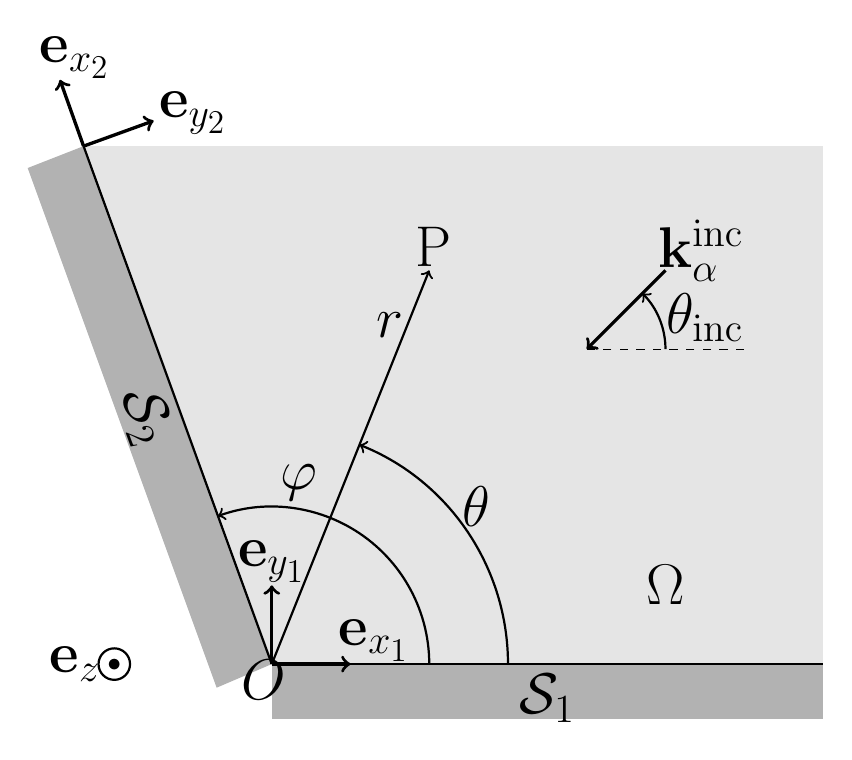
\begin{tikzpicture}
	\fill[color=gray!20] (0,0) -- (7,0)  -- (7,6.5778) -- (-2.39,6.5778) -- cycle;  
	\draw[ thick, ->] (2,0) arc (0:110:2);
	
	\fill[color=gray!60] (0,0) -- (7,0)  -- (7,-0.7) -- (0,-0.7) -- cycle;  
	
	\fill[color=gray!60] (0,0) --  (-2.39,6.5778) --(-3.1,6.3) -- (-0.7,-0.3) -- cycle; 
	
	
	\draw[thick, color = black]  (0,0) -- (7,0) node[midway,below] {\huge $\mathcal{S}_1$ };
	
	\draw[thick, color = black]  (0,0) -- (-2.39,6.5778) node[midway,below,sloped] { \huge $\mathcal{S}_2$};
	
	\draw[very thick, ->] (-2.39,6.5778) -- (-2.69,7.42);
	
	\node[scale=1] at (-2.5,7.7){ \huge $\mathbf{e}_{x_2}$};
	
	\draw[very thick, ->] (-2.39,6.5778) -- (-1.5,6.9);
	
	\node at (-1,7){\huge $\mathbf{e}_{y_2} $};
	
	
	\node at (0.35,2.3){\huge $\varphi$} ; 
	
	\draw[very thick, ->] (0,0) -- (1,0);
	
	\node at (1.3,0.3) {\huge $\mathbf{e}_{x_1} $};
	
	\draw[very thick, ->] (0,0) -- (0,1);
	
	\node at (0,1.3){\huge $\mathbf{e}_{y_1} $};
	
	\node at (-2,-0.01) {$\bullet$};
	
	\draw[thick] (-2,0) circle (0.2);
	
	\node at (-2.5,0){\huge $\mathbf{e}_{z}$};
	
	\draw[very thick, ->] (5,5) -- (4,4);
	
	\draw[dashed] (6,4) -- (4,4);
	
	\draw[thick, ->] (5,4) arc (0:45:1);
	
	\node at (5.5,4.4){\huge $\theta_{\rm inc}$};
	
	\node at (5.45,5.25){\huge $\mathbf{k}^{\rm inc}_{\alpha}$};
	
	\node at (-0.1,-0.2){\huge $O$};
	
	\node at (5,1){\huge $\Omega$ };
	
	\draw[thick, ->] (0,0) -- (2,5); 
	
	\draw[thick, ->] (3,0) arc (0:68.2:3);
	
	\node at (2.6,2){\huge $\theta$};
	
	\node at (1.5,4.3){\huge $r$};
	
	\node at (2.06,5.3){\huge P};
	
	\end{tikzpicture}
    }
	\caption{Plane wave incident on a stress-free wedge of angle $\varphi$ }
        \label{wedge}
\end{figure}
Let us consider the diffraction problem of a plane longitudinal elastic wave $\mathbf{u}^{inc}$ incident on a wedge delimited by the stress-free infinite plane faces $\mathcal{S}_1$ and $\mathcal{S}_2$. The inside of the wedge is a homogeneous isotropic medium occupying the space $\Omega$ defined by :
\begin{equation}
\Omega=\{ (r\cos \theta, r \sin \theta) \backslash \theta \in \rbrack 0, \varphi \lbrack \} 
\end{equation}
And the incident plane wave is of the form
\begin{equation}
\mathbf{u}^{inc}(\mathbf{x},t)=\mathbf{A}_{\alpha}e^{i(\mathbf{k}_{\alpha}^{inc}\cdot \mathbf{x}-\omega t)}
\end{equation}
$\alpha=L,T$ is the type of the incident plane wave (longitudinal or transversal), $\mathbf{A}_{\alpha}$ is the amplitude vector and $\mathbf{k}_{\alpha}^{inc}$ is the incident wave vector. The Cartesian coordinate system $(O; \mathbf{e}_{x_1}, \mathbf{e}_{y_1} )$ is linked to the face $\mathcal{S}_1$ of the wedge and $(O;  \mathbf{e}_{x_2}, \mathbf{e}_{y_2} )$ is linked to the face $\mathcal{S}_2$, as shown in Fig.~\ref{wedge}. These coordinate systems have the same origin located on the wedge edge which coincides with the $z$-axis. Let $\mathbf{x} = (x'_1,y'_1)_{ (\mathbf{e}_{x_1}, \mathbf{e}_{y_1}) } = (x'_2,y'_2)_{ (\mathbf{e}_{x_2}, \mathbf{e}_{y_2})}$ be a position vector $\mathbf{x} = (r,\theta)$ in a local basis of polar coordinates associated to the coordinates $(x'_1,y'_1)$. In the following, except when specified otherwise, all vectors are expressed in the coordinate system  $(O; \mathbf{e}_{x_1}, \mathbf{e}_{y_1} )$. The incident wave vector is given by 
\begin{equation}
\mathbf{k}_{\alpha}^{inc}=\frac{\omega}{c_{\alpha}} 
\begin{pmatrix}
\cos\theta_{inc} \\ 
\sin\theta_{inc} 
\end{pmatrix}
\end{equation}
$c_L=\sqrt{(\underline{\lambda}+2\underline{\mu})/\rho}$ is the velocity of the longitudinal waves,  $c_T=\sqrt{\underline{\mu}/\rho}$ is the velocity of the transversal ones and $\underline{\lambda}, \underline{\mu}$ are the Lam\'{e} coefficients. The amplitude vector may be colinear (in the case of a longitudinal wave) or normal (in the case of a transversal wave) to the incident wave vector. It will then be directed by $\mathbf{\hat{i}_L}$ or $\mathbf{\hat{i}_{T}}$ respectively :
\begin{equation}
\mathbf{\hat{i}_L} = \begin{pmatrix}
\cos\theta_{inc} \\ \sin\theta_{inc}
\end{pmatrix}
~~~~
\mathbf{\hat{i}_{T}} = \begin{pmatrix}
-\sin\theta_{inc} \\ \cos\theta_{inc}
\end{pmatrix}
\label{ivec}
\end{equation}
In all the following, bold characters are reserved for matrices in order to simplify notations and the time-harmonic factor $e^{-i\omega t}$ is omitted.

The unknown displacement field $u$ is a solution of the linear elasticity equations for a homogeneous isotropic medium and verifies stress-free boundary conditions on the wedge faces. Let us suppose that the total displacement field is the sum of an incident and a scattered field :
\begin{equation}
u=u_0+u^{inc}
\end{equation}
The dimensionless problem is obtained thanks to the following change in variables :
\begin{subequations}
\begin{equation}
x=\frac{\omega}{c_L} x', \hspace{1em} y=\frac{\omega}{c_L} y'
\end{equation}
\begin{equation}
u_0(x',y')=v(x,y)
\end{equation}
\label{adim}
\end{subequations}
The problem that we wish to solve is the following :

\begin{equation}
(\mathcal{P}^{\alpha}) \hspace{2em} \left\{~~
\begin{matrix}
(E+1)v=0 & (\Omega) \\
Bv=-B \rm v_{\alpha}^{inc} & (\mathcal{S})
\end{matrix}
\right.
\label{Padim}
\end{equation}
where $E$ and $B$ are respectively the elasticity and normal stress operators:
\begin{gather}
Ev=\mu \Delta v +(\lambda+\mu) \nabla \, \nabla v \label{defE}\\
Bv=(\lambda \nabla v .\mathbf{\mathbb{I}_2}+2\mu \mathbf{\varepsilon} (v)).n\label{defB}
\end{gather}
$\mathbb{I}_2$ is the two-dimensional identity matrix and $n$ is the inward normal to the faces of the wedge ($n=e_{y_j}$ on $\mathcal{S}_j$). The dimensionless Lam\'{e} coefficients are given by
\begin{equation}
\lambda=\frac{\underline{\lambda}}{\rho c_L^2}, \; \; \; \; \mu=\frac{\underline{\mu}}{\rho c_L^2}
\label{LameAdim}
\end{equation}
The deformations tensor is given by 
\begin{equation}
\varepsilon(v)=\dfrac{1}{2}\begin{pmatrix}
2\dfrac{\partial v_1}{\partial x} & \dfrac{\partial v_1}{\partial y}+\dfrac{\partial v_2}{\partial x} \\
\dfrac{\partial v_1}{\partial y}+\dfrac{\partial v_2}{\partial x}& 2\dfrac{\partial v_2}{\partial y}
\end{pmatrix}
\end{equation}
where $(v_1,v_2)$ are the components of vector $v$ and the dimensionless incident waves are
\begin{equation}
\rm v_L^{inc}(r,\theta)=\begin{pmatrix}
\cos \theta_{inc} \\
\sin \theta_{inc}
\end{pmatrix} e^{ir\nu_L \cos(\theta-\theta_{inc})}
\hspace{2em}
\rm v_T^{inc}(r,\theta)=\begin{pmatrix}
-\sin \theta_{inc} \\
\cos \theta_{inc}
\end{pmatrix} e^{ir\nu_T \cos(\theta-\theta_{inc})} 
\end{equation}
Finally, let us define the following ratios :
\begin{equation}
\nu_L=1 \hspace{2em} \nu_T=\frac{c_L}{c_T} \hspace{2em} \nu_R=\frac{c_L}{c_R} ,
\label{nuLnuT}
\end{equation}
where $c_R$ is the Rayleigh wave velocity.

\section{Integral Formulation of the solution}
The first step in solving problem $(\mathcal{P}^{\alpha})$ is to formulate the solution as an integral, following the formalism of Kamotski and Lebeau \cite{KamotskiLebeau}. In order to do so, a new class of functions is defined, as well as the outgoing solution of the problem. The main ideas of their development are reproduced here.
\subsection{Limiting absorption principle}
The limiting absorption principle is applied to $(\mathcal{P}^{\alpha})$, meaning that it is considered as a special case ($\varepsilon=0$ i.e. no medium absorption) of the problem
\begin{equation}
(\mathcal{P}^{\alpha}_{\varepsilon}) \hspace{2em} \left\{~~
\begin{matrix}
(E+e^{-2i\varepsilon})v^{\varepsilon}=0 & (\Omega) \\
Bv^{\varepsilon}=-B \rm v_{\alpha}^{inc} & (\mathcal{S})
\end{matrix}
\right.
\label{Pabs}
\end{equation}
Kamotski and Lebeau \cite{KamotskiLebeau} have shown that this problem admits a unique solution, which is the sum of two contributions, corresponding to each of the faces of the wedge
\begin{equation}
v^{\varepsilon}=v_1^{\varepsilon}+v_2^{\varepsilon},
\label{v1+v2}
\end{equation}
where functions $v_j^{\varepsilon}$ are defined in all of $\mathbb{R}^2$ by
\begin{equation}
v_j^{\varepsilon}=-(E+e^{-2i\varepsilon})^{-1} \begin{bmatrix}
\begin{pmatrix}
\alpha_j \\
\beta_j
\end{pmatrix}
\otimes \delta_{\mathcal{S}_j}
\end{bmatrix},
\label{vjdef}
\end{equation}
where $\delta_{\mathcal{S}_j}$ is the Dirac distribution associated to face $\mathcal{S}_j$. It is defined by its action on an arbitrary test function $f \in C_0^{\infty}(\mathbb{R}^2)$ :
\begin{equation}
\langle \delta_{\mathcal{S}_j},f\rangle=\int_0^{\infty}f((x_j,0)\, dx_j
\label{defDirac}
\end{equation}
The distributions $\alpha_j$ and $\beta_j$ are unknown and are supposed to belong to the special class $\mathcal{A}$ defined hereafter.
%\begin{mydef}
%We say that $f \in \mathcal{A}$ if $f \in \mathcal{S}'(\mathbb{R}), \mbox{supp} f \subset \mathbb{R}_+$ and
%\begin{gather}
% \exists C_0>0 \mbox{ such that } \underset{-\pi<\theta<0}{sup} \int_{C_0}^{+\infty}|\hat{f}(\rho e^{i\theta})|^2\,d\rho <+\infty \\
%\hat{f} \mbox{ is holomorphic in neighborhoods of } \nu_L, \nu_T, \nu_R.
%\end{gather}
% \label{defA}
%\end{mydef}
The notation $\hat{f}$ refers to the Fourier transform of the function $f$:
\begin{equation}
\hat{f}(\xi)=\int_{\mathbb{R}}e^{-ix\xi}f(x)\,dx
\label{defFouriersimple}
\end{equation}
and $\mathcal{S}'(\mathbb{R})$ is the space of tempered distributions on $\mathbb{R}$. Using this definition, Kamotski and Lebeau \cite{KamotskiLebeau} then obtain the following:
%\begin{lemme}
%Suppose $\alpha_j, \beta_j \in \mathcal{A}, j=1,2$. Then the two tempered distributions $v_j^{\varepsilon}$ defined by (\ref{vjdef}) converge in $\mathcal{S}'(\mathbb{R})$ when $\varepsilon \rightarrow 0$ towards two tempered distributions $v_j^0 \in \mathcal{S}'(\mathbb{R})$ which solve
%\begin{equation}
%(E+1)v_j^0=-
%\begin{pmatrix}
%\alpha_j \\
%\beta_j
%\end{pmatrix}
%\otimes \delta_{\mathcal{S}_j}
%\end{equation}
%Furthermore, the following properties are true for all $\varepsilon \in \lbrack 0,\pi \lbrack $:
%\begin{description}
%  \item[(i)] $v_j^{\varepsilon}$ are continuous in $\mathbb{R}^2$
%  \item[(ii)] in polar coordinates $(r,\theta)$, we have
%  \begin{gather}
% v_j^{\varepsilon} \in C(\lbrack 0,2\pi \rbrack; H^1_{loc}(\mathbb{R}_+))\\
% \frac{1}{r}\frac{\partial v_j^{\varepsilon}}{\partial \theta}\in C(\lbrack0,2\pi\rbrack;L^2_{loc}(\mathbb{R}_+))
%\end{gather}
%\end{description}
%\end{lemme}
%Finally, this lemma justifies the following definition
%\begin{mydef}
%We call $v$  an outgoing solution of  $(\mathcal{P}^{\alpha})$ if $v$ is a solution of the form
%\begin{equation}
%v=v_1+v_2,
%\end{equation}
%with
%\begin{equation}
%v_j=-\underset{\varepsilon\rightarrow0}{lim}(E+e^{-2i\varepsilon})^{-1} \begin{bmatrix}
%\begin{pmatrix}
%\alpha_j \\
%\beta_j
%\end{pmatrix}
%\otimes \delta_{\mathcal{S}_j}
%\end{bmatrix},
%\end{equation}
%where $\alpha_j,\beta_j \in\mathcal{A},j=1,2$.
%\end{mydef}
Existence and uniqueness of the outgoing solution was demonstrated by Kamotski and Lebeau \cite{KamotskiLebeau} and is not the object of this paper. Our goal is to propose a detailed method of numerical computation of this solution.

The limiting absorption principle presented above leads to a rigorous definition of the solution to the problem $(\mathcal{P}^{\alpha})$. It is also useful in order to derive an integral formulation of this solution.
\subsection{Integral formulation}
In order to compute the integral formulation of the solution, the two-sided Fourier transform of a tempered distribution and its inverse are defined in the following manner :
\begin{subequations}
\begin{equation}
\hat{f}(\xi,\eta)=\int \int_{\mathbb{R}^2}f(x,y)e^{-i(x\xi+y\eta)}\, {\rm d}x {\rm d}y
\label{fourierdef}
\end{equation}
\begin{equation}
f(x,y)=\frac{1}{4\pi^2}\int\int_{\mathbb{R}^2} \hat{f}(\xi,\eta)e^{i(x\xi+y\eta)}\rm d\xi \rm d\eta
\label{invfourierdef}
\end{equation}
\label{fullfourierdef}
\end{subequations}
The first step is to take the two-sided Fourier transform of equation \eqref{vjdef}. This is permitted since all the encountered distributions are tempered distributions (as discussed in the previous subsection).
\begin{equation}
\hat{v}^{\epsilon}_j(\xi,\eta)=(\mathbf{M}-e^{-2i\varepsilon}\mathbf{\mathbb{I}_2})^{-1}\Sigma_j(\xi),
\label{matMvjeps}
\end{equation}
where $\Sigma_j, \, j=1,2$  are two unknown functions called the spectral functions such that
\begin{equation}
\Sigma_j(\xi)=\begin{pmatrix}
\hat{\alpha_j}(\xi)\\ \hat{\beta_j}(\xi)
\end{pmatrix},
\end{equation}
and the matrix
\begin{equation}
\mathbf{M}=
\begin{pmatrix}
(\lambda+\mu)\xi^2+\mu(\xi^2+\eta^2) & (\lambda+\mu)\xi \eta \\
 (\lambda+\mu)\xi \eta & (\lambda+\mu)\eta^2+\mu(\xi^2+\eta^2)
\end{pmatrix}
\label{matM}
\end{equation}
is the two-sided Fourier transform of the elasticity operator $E$ defined by \eqref{defE}. By using the fact that $\lambda+2\mu=1$ and $\mu=1/\nu_T^2$ and by substituting \eqref{matM} into \eqref{matMvjeps}, functions $\hat{v}^{\epsilon}_j$ can be expressed as:
\begin{equation}
\hat{v}^{\varepsilon}_j(\xi,\eta)=\begin{pmatrix}
a(\xi,\eta) & b(\xi,\eta) \\
b(\xi,\eta) & a(\eta,\xi)
\end{pmatrix} \Sigma_j(\xi),
\end{equation}
where
\begin{subequations}
\begin{equation}
a(\xi,\eta)=\frac{\xi^2+\nu_T^2 \eta^2-\nu_T^2e^{-2i\varepsilon}}{(\xi^2+\eta^2-e^{-2i\varepsilon})(\xi^2+\eta^2-\nu_T^2e^{-2i\varepsilon})}
\end{equation}
\begin{equation}
b(\xi,\eta)=\frac{(1-\nu_T^2)\xi \eta}{(\xi^2+\eta^2-e^{-2i\varepsilon})(\xi^2+\eta^2-\nu_T^2e^{-2i\varepsilon})}
\end{equation}
\end{subequations}
The two-sided Fourier transform of $v_j^{\varepsilon}$ can now be reversed
\begin{equation}
v_j^{\varepsilon}(x_j,y_j)=\frac{1}{4\pi^2}\int_{- \infty}^{+ \infty} e^{ix_j\xi} \int_{-\infty}^{+\infty}e^{iy_j\eta}\begin{pmatrix}
a(\xi,\eta) & b(\xi,\eta) \\
b(\xi,\eta) & a(\eta,\xi)
\end{pmatrix} \,d\eta\, \Sigma_j(\xi) \,d\xi
 \label{invdouble}
\end{equation}
The inner integral is computed using Gauss' residue theorem. The poles of the integrand are $\eta=\pm \zeta_*^{\varepsilon}(\xi), *=L,T$, with
\begin{equation}
\zeta_*^{\varepsilon}(\xi)=\sqrt{e^{-2i\varepsilon}\nu_*^2-\xi^2}
\label{defzetaeps}
\end{equation}
thus yielding:
\begin{equation}
v_j^{\varepsilon}(x_j,y_j)=\frac{i}{4\pi}e^{2i\varepsilon}\int_{-\infty}^{+\infty} e^{ix_j\xi}\sum_{*=L,T}e^{i|y_j|\zeta_*^{\varepsilon}(\xi)}M_*^{\varepsilon}(\xi,\mbox{sgn }y_j)\Sigma_j(\xi)\,d\xi,
\label{vjeps}
\end{equation}
where, noting $t=\mbox{sgn }y_j$
\begin{equation}
\mathbf{M_L^{\varepsilon}}(\xi,t)=\begin{pmatrix}
\frac{\xi^2}{\zeta_L^{\varepsilon}(\xi)} &t\xi \\
t\xi & \zeta_L^{\varepsilon}(\xi)
\end{pmatrix}
~~\mbox{  and  }~~
\mathbf{M_T^{\varepsilon}}(\xi,t)=\begin{pmatrix}
\zeta_T^{\varepsilon}(\xi) & -t\xi \\
-t\xi & \frac{\xi^2}{\zeta_T^{\varepsilon}(\xi)}
\end{pmatrix}
\label{M*eps}
\end{equation}
According to Croisille and Lebeau \cite{CroisilleLebeau}, after slightly deforming the integration contour from $\mathbb{R}$ to $\Gamma_0$ represented in Fig. \ref{gamma0} integral \eqref{vjeps} converges when $\varepsilon \rightarrow 0$: 
\begin{equation}
v_j(x_j,y_j)=\frac{i}{4\pi}\int_{\Gamma_0} e^{ix_j\xi}\sum_{*=L,T}e^{i|y_j|\zeta_*(\xi)}\mathbf{M_*}(\xi,\mbox{sgn }y_j)\Sigma_j(\xi)\,d\xi
\label{vj0}
\end{equation}
In order to simplify notations, the exponent $\epsilon=0$ has been omitted.
The function $\zeta_*$ defined by taking $\epsilon=0$ in \eqref{defzetaeps} has multiple branch cuts. In order to satisfy the radiation condition at infinity
\begin{equation}
\lim\limits_{|y_j| \rightarrow +\infty} |v_j^{\varepsilon}(x_j,y_j)|=0,
\label{CR}
\end{equation}
we chose Im $\zeta_*(\xi)>0$ :
\begin{equation}
\zeta_*(\xi)=
\left\{
\begin{matrix}
i\sqrt{\xi^2-\nu_*^2}& \mbox{for } |\xi| \geq \nu_* \\
-\sqrt{\nu_*^2-\xi^2}& \mbox{for } |\xi| \leq \nu_*
\end{matrix}
\right.
\label{defzeta}
\end{equation}

The integral formulation \eqref{vj0} is an expression of the solution in terms of an unknown function $\Sigma_j$ called the spectral function. In the next section, by computing a far-field asymptotic approximation of this integral, we define a function of the observation angle $\theta$ (see Fig. \ref{wedge}) called the diffraction coefficient and express this coefficient in terms of $\Sigma_1$ and $\Sigma_2$.

\begin{figure}[h]
\centering
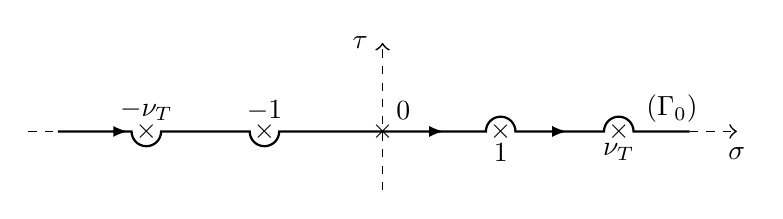
\begin{tikzpicture}[scale=0.75]
\node at (0,0) {$\times$};
\node at (0.35,0.35) {$0$};
\node at (2,0) {$\times$}; % Pole
\node at (4,0) {$\times$}; %pole
\node at (2,-0.35) {$1$};
\node at (4,-0.35) {$\nu_T$};
\node at (-2,0) {$\times$};
\node at (-4,0) {$\times$};
\node at (-2,0.35) {$-1$}; %pole
\node at (-4,0.35) {$-\nu_T$}; %pole
\node at (4.9,0.38) {$(\Gamma_0)$};
\node at (6,-0.38) {$\sigma$};
\node at (-0.38,1.5){$\tau$};

\draw[dashed,yshift=0pt]
(-6,0)--(-5.5,0);

\draw[dashed, yshift=0pt,decoration={ markings,  mark=at position 1 with {\arrow[scale=1.5]{>}}},
      postaction={decorate}]
(5.2,0)--(6.0,0);

\draw[dashed, yshift=0pt,decoration={ markings,  mark=at position 1 with {\arrow[scale=1.5]{>}}},
      postaction={decorate}]
      (0,-1)--(0,1.5);

\draw[thick,black,yshift=0pt,
decoration={ markings,  % This schema allows for fine-tuning the positions of arrows 
      mark=at position 0.1 with {\arrow{latex}},
      mark=at position 0.6 with {\arrow{latex}},
      mark=at position 0.8 with {\arrow{latex}}},
      postaction={decorate}]
      (-5.5,0) -- (-4.25,0)  arc (-180:0:0.25) -- (-2.25,0)  arc (-180:0:0.25)  -- (1.75,0)arc (180:0:0.25)  -- (3.75,0)arc (180:0:0.25) -- (5.2,0); % ca c'est l'axe
\end{tikzpicture}
\caption{Integration contour $\Gamma_0$ in the complex plane $\xi=\sigma+i\tau$.}
\label{gamma0}
\end{figure}

\subsection{Far-field asymptotics}
\label{farfield}
Let $P=(x',y')=(r\cos\theta,r\sin\theta)$ be an observation point, represented in Fig. \ref{wedge}. According to equation \eqref{adim}, the diffracted field at P is given by:
\begin{equation}
u_0(x',y')=v(\frac{\omega}{c_L}r\cos\theta,\frac{\omega}{c_L}r\sin\theta)
\end{equation}
Let $R=\frac{\omega r}{c_L}$ denote the far-field parameter. Our goal is to determine an asymptotic evaluation of the diffracted field when $R\rightarrow +\infty$. To do so, we begin by applying the following change of variables in integral \eqref{vj0} :
\begin{equation}
\begin{split}
 \xi&=\nu_*\cos\lambda \\
 d\xi&=-\nu_*\sin\lambda\, d\lambda,
\end{split}
\label{changevar2}
\end{equation}
yielding, in polar coordinates
\begin{equation}
v_1(r\cos\theta,r\sin\theta)=\frac{i}{4\pi} \int_{C_0}\sum_{*=L,T}\nu_*^2 e^{i\nu_*r\cos(\lambda+\bar{\theta})}\mathbf{ P_*}(\lambda,t)\Sigma_1(\nu_*\cos\lambda) \, d \lambda,
\label{v1pol}
\end{equation}
where $t=\rm sgn \sin \theta$,
\begin{equation}
\bar{\theta}=\left\{
\begin{matrix}
\theta & \rm if \theta \leq \pi \\
2\pi-\theta & \rm if \theta>\pi
\end{matrix}
\right. ,
\label{C3:thetatilde}
\end{equation}
contour $C_0$ is represented in Fig. \ref{steepestcontour} and
\begin{gather}
\mathbf{P_L}(\lambda,t)=
\begin{pmatrix}
\cos^2\lambda & -t\cos\lambda\sin\lambda \\
-t\cos\beta\sin\lambda & \sin^2\lambda
\end{pmatrix}\\
\mathbf{P_T}(\lambda)=\mathbf{\mathbb{I}_2}-\mathbf{P_L}(\lambda)
\end{gather}
Note that $\mathbf{P_*}(\lambda,-1)=\mathbf{P_*}(-\lambda,1)$. In the following, we will use the notation $\mathbf{P_*}(\lambda)=\mathbf{P_*}(\lambda,1)$.

An asymptotic evaluation of \eqref{v1pol} is determined using the steepest descent method. This consists of deforming integration contour $C_0$ into $\gamma_{\bar{\theta}}$ represented in Fig. \ref{steepestcontour}. The approximation is then the sum of two contributions:
\begin{equation}
v_1=v_1^{sing}+v_1^{diff},
\end{equation}
where $v_1^{sing}$ is the contribution of all the singularities of the spectral function $\Sigma_1$ crossed by the contour deformation and $v_1^{diff}$ is the contribution of the phase function's saddle point $\lambda_s=\pi-\bar{\theta}$, corresponding to the field diffracted by the wedge edge. We will see that the singularities crossed are either simple poles (corresponding to the reflected waves on the wedge faces or to the Rayleigh surface waves) or branch points (corresponding to head waves). In this paper, we are only concerned with the determination of the edge-diffracted field, which corresponds to the contribution of the saddle-point and is given by:
\begin{equation}
v_1^{diff}(r\cos\theta,r\sin\theta)=\frac{e^{-i\pi/4}}{2\sqrt{2\pi}}\sum_{*=L,T}\nu_*^2\frac{e^{-i\nu_*r}}{\sqrt{\nu_*r}}\mathbf{P_*}(\pi-\theta)\Sigma_1(-\nu_*\cos\theta)
\label{v1diff}
\end{equation}
Note that asymptotic evaluation \eqref{v1diff} is only valid when the saddle point $\lambda_s$ does not coincide with a singular point (pole or branch point) of the spectral function $\Sigma_1$. The poles of the spectral functions will be determined analytically in section \ref{singpart}. The branch points of the spectral functions are located at $\xi=\pm \nu_L$ and $\xi = \pm \nu_T$. Applying \eqref{changevar2}, this means that :
\begin{subequations}
\begin{equation}
\nu_*\cos\lambda_s=-\nu_*\cos\theta=\pm \nu_L=\pm 1
\label{eqbranch1}
\end{equation}
\begin{equation}
\rm or \hspace{1em} \nu_*\cos\lambda_s=-\nu_*\cos\theta=\pm \nu_T
\label{eqbranch2}
\end{equation}
\label{eqbranch}
\end{subequations}
For $*=L$, \eqref{eqbranch1} yields $\theta=0$ or $\theta=\pi$, meaning that the direction of observation is along the wedge's horizontal face $\mathcal{S}_1$. \eqref{eqbranch2} does not have a solution for $*=L$. For $*=T$, \eqref{eqbranch1} yields $\theta=\theta_c=\rm acos(1/\nu_T)$ or $\theta=\pi- \theta_c$, $\theta_c$ is called the critical angle, and \eqref{eqbranch2} yields $\theta=0$ or $\theta=\pi$. Borovikov \cite{Borovikov} gives some clues as to how to treat the case where the stationary phase point coincides with another singularity of the integrand. In this paper, it is assumed that $\lambda_s$ does not coalesce with a singularity of the integrand.

Similar considerations yield:
\begin{equation}
v_2^{diff}(x_2,y_2)=\frac{e^{-i\pi/4}}{2\sqrt{2\pi}}\sum_{*=L,T}\nu_*^2\frac{e^{-i\nu_*r}}{\sqrt{\nu_*r}}\mathbf{P_*}(\pi-(\varphi-\theta))\Sigma_2(-\nu_*\cos(\varphi-\theta))
\label{v2diff}
\end{equation}
The branch points are now located at $\bar{\theta}=\varphi$, $\bar{\theta}=\pi-\varphi$, $\bar{\theta}=\varphi-\theta_c$ and $\bar{\theta}=\pi-(\varphi-\theta_c)$.
The total diffracted field is the sum of the saddle-point contributions from each face
\begin{equation}
v^{diff}=v_1^{diff}+v_2^{diff}
\label{vdiff12}
\end{equation}
This can be identified with the total diffracted field written in terms of longitudinal and transversal contributions, 
\begin{equation}
v^{diff}=v^{diff}_L \hat{i}_L+v^{diff}_T \hat{i}_T,
\label{vdiffLT}
\end{equation}
with $\hat{i}_*$ defined by \eqref{ivec}, leading to the following definition of the diffraction coefficient $D_{\beta}^{\alpha}$ : 
\begin{equation}
v_{\beta}^{diff}(r\cos\theta,r\sin\theta)=D_{\beta}^{\alpha}(\theta)\frac{e^{-i\nu_{\beta}r}}{\sqrt{\nu_{\beta}r}} \rm v^{\alpha}_{inc}(r\cos\theta,r\sin\theta),
\label{defcoeffdiff}
\end{equation}
where $\beta=L,T$ is the type of the diffracted wave. The diffracted field is thus represented by a cylindrical wave, proportional to the incident wave and weighted by the diffraction coefficient. By substituting \eqref{v1diff}-\eqref{v2diff} into \eqref{vdiff12} and \eqref{defcoeffdiff} into \eqref{vdiffLT} and identifying the results, we finally obtain the expression of the diffraction coefficients in terms of the components $(\hat{\alpha}_j,\hat{\beta}_j), \, \, j=1,2$ of the spectral functions
\begin{gather}
\begin{split}
 D^{\alpha}_L(\theta)=\frac{e^{-i\pi/4}}{2\sqrt{2\pi}}&\big(\hat{\alpha}_1(-\cos\theta)\cos\theta+\hat{\beta}_1(-\cos\theta)\sin\theta\\
&+\hat{\alpha}_2(-\cos(\varphi-\theta))\cos(\varphi-\theta)+\hat{\beta}_2(-\cos(\varphi-\theta))\sin(\varphi-\theta)\big)
\end{split} \label{DL}\\
\begin{split}
 D^{\alpha}_T(\theta)=\nu_T^2\frac{e^{-i\pi/4}}{2\sqrt{2\pi}}&\big(-\hat{\alpha}_1(-\nu_T\cos\theta)\sin\theta+\hat{\beta}_1(-\nu_T\cos\theta)\cos\theta\\
&+\hat{\alpha}_2(-\nu_T\cos(\varphi-\theta))\sin(\varphi-\theta)-\hat{\beta}_2(-\nu_T\cos(\varphi-\theta))\cos(\varphi-\theta)\big) 
\end{split} \label{DT}
\end{gather}

\begin{figure}
\centering
\resizebox{!}{0.2\textheight}{
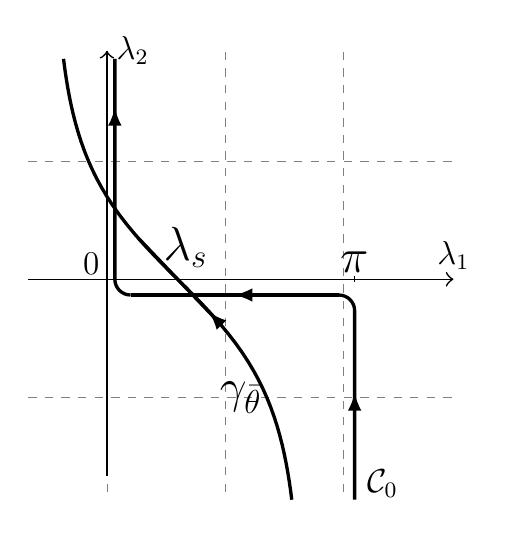
\begin{tikzpicture}
\draw[step=1.5cm,gray,very thin,dashed](-1,-2.7)grid(4.4,2.9);
%\draw[thin](-1,0)-- (0,0);
\draw[thin,decoration={ markings, mark=at position 1 with {\arrow[scale=1.5]{>}}},
      postaction={decorate}] (-1,0)  -- (4.4,0) node[above]{\large $\lambda_1$};
%\drawn[thin] -- (pi+1,0) node[below]{$\sigma$};
\draw[thin,decoration={ markings, mark=at position 1 with {\arrow[scale=1.5]{>}}},
      postaction={decorate}](0,-2.5)--(0,2.9) node[right]{\large $\lambda_2$};
\foreach \x in {pi} {  
  \draw (\x,-1pt) -- (\x,1pt) node[pos=0,above] {\LARGE $\pi$};
  }

\node at (-0.2,0.2) {\large $0$};
\node at (1,0.4) {\LARGE $\lambda_s$};
%\node at (3.5,-3.8) {$(\mathcal{C}_\xi)$};
\node at (3.5,-2.6) {\large $\mathcal{C}_0$};
\node at (1.7,-1.5) {\LARGE $\gamma_{\bar{\theta}}$};

\draw[black,very thick][domain=0:2.8] plot({2*pi/7 - acos(1/cosh(\x))*pi/180},\x);
\draw[black,very thick][domain=-2.8:0] plot({2*pi/7 + acos(1/cosh(\x))*pi/180},\x);
\draw[very thick,black,xshift=0pt,
decoration={ markings,  % This schema allows for fine-tuning the positions of arrows 
      mark=at position 0.8 with {\arrow{latex}}},
      postaction={decorate}]
      (0.3,-0.2) arc (270:180:0.2) -- (0.1,2.8); 
\draw[very thick,black,yshift=0pt,
decoration={ markings,  % This schema allows for fine-tuning the positions of arrows 
      mark=at position 0.5 with {\arrow{latex}}},
      postaction={decorate}]
      (pi-0.2,-0.2) -- (0.3,-0.2) ;
%\draw[very thick] (0.3,0) arc (270:180:0.2);

\draw[very thick,black,xshift=89.5pt,
decoration={ markings,  % This schema allows for fine-tuning the positions of arrows 
      mark=at position 0.5 with {\arrow{latex}}},
      postaction={decorate}]
      (0,-2.8) -- (0,-0.4) arc (0:90:0.2) ;
      \draw[very thick,black,
decoration={ markings,  % This schema allows for fine-tuning the positions of arrows 
      mark=at position 0.1 with {\arrow{latex}}},
      postaction={decorate}]
      (1.3988,-pi/6)  -- (0.3964,pi/6);  
\end{tikzpicture}
}
\caption{Integration contours $C_0$ and $\gamma_{\bar{\theta}}$ in the complex plane $\lambda=\lambda_1+i\lambda_2$. $\lambda_s$ is the stationary phase point.}
\label{steepestcontour}
\end{figure}

In order to determine the field diffracted by a wedge illuminated by an incident plane wave, it is sufficient to compute the diffraction coefficient. This coefficient has been expressed in terms of two unknown functions called the spectral functions. The semi-analytical computation of these functions is presented in the following section

\section{Semi-analytical evaluation of the spectral functions}
\label{section4}
The first step in computing the spectral functions is to determine a system of functional equations of which they are a solution. We will then show that these functions can be decomposed into two parts : a singular function, computed analytically, and a regular function, approached numerically.
\subsection{Functional equations}
In the previous section, the diffracted wave has been expressed in terms of two unknown functions called the spectral functions. In this subsection, a system of functional equations satisfied by these functions is determined.

The system of functional equations is determined using the boundary conditions on the faces of the wedge \eqref{Padim}. These can be expressed separately for each face of the wedge, using decomposition \eqref{v1+v2}:
\begin{equation}
\left\{
\begin{matrix}
B \big( v_1(x_1,0)+v_2(x_2 \cos \varphi, x_2 \sin \varphi) \big) = -B \rm v_{\alpha}^{inc}|_{\mathcal{S}_1} \\
B \big( v_2(x_2,0)+v_1(x_1 \cos \varphi, x_1 \sin \varphi) \big) = -B \rm v_{\alpha}^{inc}|_{\mathcal{S}_2}
\end{matrix}
\right.
\label{Bivi}
\end{equation}
Let us note  $(v_j^1,v_j^2),\, j=1,2$ the coordinates of vector $v_j$ in the Cartesian coordinate system $(x_j,y_j)$, represented in Fig.~\ref{wedge}.
By expliciting the normal stress operator \eqref{defB} in each of these systems,  system (\ref{Bivi}) can be expressed as
\begin{equation}
\left\{
\begin{array}{l}
B_1(v_1)+B_2(v_2)=-B\rm v_*^{inc}|_{\mathcal{S}_1} \\
B_1(v_2)+B_2(v_1)=-B\rm v_*^{inc}|_{\mathcal{S}_2}
\end{array}
\right.,
\end{equation}
where two new operators are defined:
\begin{gather}
B_1(v_1)=
\begin{pmatrix}
\mu \left( \frac{\partial v_1^1}{\partial y_1}+\frac{\partial v_1^2}{\partial x_1} \right) \\
~\\
\frac{\partial v_1^2}{\partial y_1}+\lambda \frac{\partial v_1^1}{\partial x_1}
\end{pmatrix} \label{B1v1expl}\\
B_2(v_2)=
\begin{pmatrix}
\mu \sin(2\varphi)\left( \frac{\partial v_2^1}{\partial x_2}-\frac{\partial v_2^2}{\partial y_2}\right)-\mu \cos(2\varphi)  \left( \frac{\partial v_2^1}{\partial y_2}+\frac{\partial v_2^2}{\partial x_2} \right)\\
~\\
(\lambda+2\mu \sin^2\varphi) \frac{\partial v_2^1}{\partial x_2}+(\lambda+2\mu \cos^2 \varphi)\frac{\partial v_2^2}{\partial y_2}-\mu \sin(2\varphi)  \left( \frac{\partial v_2^1}{\partial y_2}+\frac{\partial v_2^2}{\partial x_2} \right)
\end{pmatrix}\label{B2v2expl}
\end{gather}

The functional equations satisfied by the spectral functions are obtained by taking the Fourier transform of this system. 

The partial derivatives of $v_1$ with respect to $x_1$ and $y_1$ are evaluated in  $y_1=0, x_1 \geq 0$ using \eqref{vj0} before being substituted into \eqref{B1v1expl}. Finally, by using the following formula
$$\int_0^{+\infty} e^{-ix(\xi-\zeta)}\,dx=\frac{1}{i(\xi-\zeta)}, \; \mbox{ Im}\xi <0, \;  \mbox{ Im} \zeta>0, $$
the Fourier transform of operator $B_1$ is obtained :
\begin{equation}
\begin{split}
\int_0^{+\infty} e^{-ix\xi}B_1(v_1)(x)\,dx&=\frac{1}{2}\textbf{DM}(\Sigma_1)(\xi) \\
&=\frac{1}{2} \int_{\Gamma_0}\textbf{DM}(\xi,\zeta)\Sigma_1(\zeta)\,d\zeta
\end{split},
\label{B1DM}
\end{equation}
with
\begin{equation}
\textbf{DM}(\xi,\zeta)=\frac{1}{2i\pi} \frac{1}{\xi-\zeta} \textbf{dm}(\zeta) =\frac{1}{2i\pi} \frac{1}{\xi-\zeta} \begin{pmatrix}
-1 & A(\zeta) \\
B(\zeta) & -1
\end{pmatrix}
\label{defDM}
\end{equation}
and
\begin{equation}
A(\zeta)=\frac{z}{\zeta_T(z)}(1-2\mu Q(\zeta)) \hspace{3em} B(\zeta)=-\frac{\zeta}{\zeta_L(\zeta)}(1-2\mu Q(\zeta)) \hspace{3em}
Q(\zeta)=\zeta_L(\zeta) \zeta_T(\zeta)+\zeta^2,
\end{equation}
where $\zeta_*,\, *=L,T$ is given by \eqref{defzeta}.


The Fourier transform of operator $B_2$ is obtained  through a similar process. The partial derivatives of $v_2$ are evaluated in $x_2=x\cos\varphi,y_2=x\sin\varphi,x\geq0$ and then substituted into \eqref{B2v2expl} before applying the Fourier transform to the results. Finally, by using the following formula
\begin{equation}
\int_0^{+\infty} e^{-ix(\xi-(\zeta \cos \varphi + \zeta_*(\xi) \sin\phiti))}\,dx=\frac{1}{i(\xi-(\zeta \cos \varphi + \zeta_*(\xi)| \sin \varphi|)}, \; \mbox{ Im}\xi <0, \;  \mbox{ Im} \zeta>0 
\end{equation}
and by noting
\begin{equation}
D_*(\xi,\zeta)=\frac{1}{\xi-(\zeta \cos \varphi + \zeta_*(\zeta) \sin\phiti)}
\end{equation}
the Fourier transform of $B_2$ is obtained :
\begin{equation}
\int_0^{+\infty} e^{-ix\xi}B_2(v_2)(x)\,dx=\frac{1}{2}\textbf{TM}(\Sigma_2)(\xi) =\frac{1}{2} \int_{\Gamma_0}\textbf{TM}(\xi,\zeta)\Sigma_2(\zeta)\,d\zeta,
\label{B2TM}
\end{equation}
where
\begin{equation}
\textbf{TM}(\xi,\zeta)=\frac{1}{2\pi i}\sum_{*=L,T}D_*(\xi,\zeta)\textbf{tm}_*(\zeta,\mbox{sgn } \sin \varphi)
\label{defTM}
\end{equation}
and, having $t = \mbox{sgn } \sin \varphi$,
\begin{gather}
\left\{
\begin{matrix}
\textbf{tm}_L(\zeta,t)=\left( \frac{\zeta}{\zeta_L(\zeta)}f_L ; \, tf_L \right) \\
f_L = \begin{pmatrix}
\mu \lbrack \cos(2\varphi)(2t\zeta\zeta_L)-\sin(2\varphi)(\zeta^2-\zeta_L^2) \rbrack \\
-\lambda+2\mu\lbrack \sin(2\varphi)(t\zeta\zeta_L) -\zeta^2 \sin^2\varphi-\zeta_L^2\cos^2\varphi \rbrack
\end{pmatrix}
\end{matrix}
\right. \label{tmL}
\\
\left\{
\begin{matrix}
\textbf{tm}_T(\zeta,t)=\left(-tf_T; \, \frac{\zeta}{\zeta_T(\zeta)} f_T\right) \\
f_T=\mu \begin{pmatrix}
\cos(2\varphi)(\zeta^2-\zeta^2_T)+\sin(2\varphi)(2t\zeta\zeta_T)\\
\sin(2\varphi)(\zeta^2-\zeta^2_T)-\cos(2\varphi)(2t\zeta\zeta_T)
\end{pmatrix}
\end{matrix}
\right. .
\label{tmT}
\end{gather}

The Fourier transform of the normal stress operator on each face of the wedge is given by a sum of these two operators. The right-hand side of the system of functional equations is obtained by computing the Fourier transform of $-Bv_{\alpha}^{inc}|_{\mathcal{S}_j},\; j=1,2$ :
\begin{equation}
\left\{
\begin{matrix}
\textbf{DM}(\Sigma_1)+\textbf{TM}(\Sigma_2)=\frac{W_1^{\alpha}}{\xi-\nu_{\alpha} \cos \theta_{inc}} \\
\textbf{TM}(\Sigma_1)+\textbf{DM}(\Sigma_2)=\frac{W_2^{\alpha}}{\xi-\nu_{\alpha}\cos(\varphi-\theta_{inc})}
\end{matrix}
\right.,
\label{equationsintegrales}
\end{equation}
where
\begin{equation}
\begin{matrix}
W_1^L=-2\begin{pmatrix}
\mu \sin 2\theta_{inc}\\
1-2\mu\cos^2\theta_{inc}
\end{pmatrix}&
W_2^L=-2\begin{pmatrix}
\mu \sin 2(\varphi-\theta_{inc}) \\
1-2\mu\cos^2(\varphi-\theta_{inc})
\end{pmatrix} \\
~
\\
W_1^T=-2 \nu_T \begin{pmatrix}
\mu \cos 2\theta_{inc}\\
\mu \sin 2\theta_{inc}
\end{pmatrix}&
W_2^T=2\nu_T \begin{pmatrix}
\mu \cos 2(\varphi-\theta_{inc})\\
\mu \sin 2(\varphi-\theta_{inc})
\end{pmatrix}
\end{matrix}
\end{equation}
Using this system of functional equations, it is possible to decompose the spectral functions into two parts : a singular function and a regular function. The first step is to extract the poles of the spectral functions.
\subsection{Singular part}
\label{singpart}
The poles and corresponding residues of the spectral functions, which lead to the reflections of the incident field on the wedge faces (these reflections can be multiple and can also lead to mode conversion) and to the fictitious fields that compensate the incident wave in the shadow zones, are computed analytically by a recursive procedure. In order to apply this procedure, it is necessary to define the following translation operator ($*=L,T$):
\begin{equation}
T_*(\xi=\nu_*\cos\theta)=\xi \cos \phiti+\zeta_*(\xi)\sin\phiti=\nu_*\cos(\theta+\tilde{\varphi}),
\end{equation}
where
\begin{equation}
\tilde{\varphi}=
\left\{
\begin{matrix}
\varphi & \mbox{ if } \varphi < \pi \\
2\pi-\varphi & \mbox{else}
\end{matrix}
\right.
\label{phitilde}
\end{equation}
This variable is useful for synthetically describing the spectral functions method for wedge angles lower and higher than $\pi$, using only one angular variable which is defined differently for each case. In order for the cosine in the translation operator to also be well defined, it is necessary to impose
\begin{equation}
\xi \in \Omega_*^+= \{ \xi=\nu_* \cos \theta, \; 0 \leq \mbox{Re} \theta < \pi-\tilde{\varphi}, \; \mbox{Im}\xi\geq0 \},
\label{defOmega0}
\end{equation}
where $\Omega_*^+$ is represented in Fig. \ref{domega0}.

\begin{figure}
\centering
\resizebox{!}{0.15\textheight}{
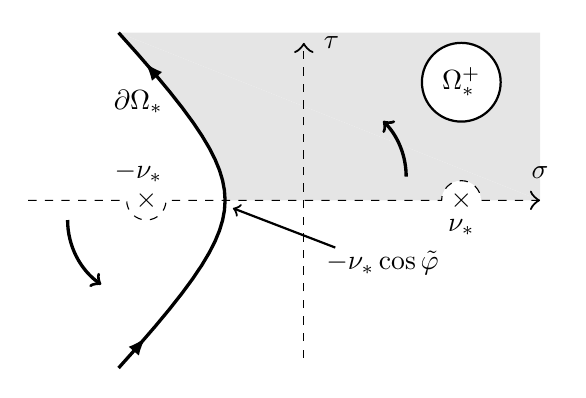
\begin{tikzpicture}
% Remplissage espace Omega_0
\fill [color=gray!20]
(-1,0)
-- plot [domain=0:1.5] ({-cosh(\x)},{sinh(\x)})
-- (3,0)
-- cycle;

\fill [color=gray!20]
({-cosh(1.5)},{sinh(1.5)})
-- plot [domain= 0:-3.0] ({-\x},{sinh(1.5)})
-- (3,0)
-- cycle;

\fill [color=white] (2,0) circle (0.25);

\node at (2,0) {$\times$}; % Pole
\node at (2,-0.35) {$\nu_*$};
\node at (-2,0) {$\times$};
\node at (-2.1,0.35) {$-\nu_*$}; %pole
\node at (3,0.35) {$\sigma$};
\node at (0.35,2) {$\tau$};
\draw[dashed,decoration={ markings, mark=at position 1 with {\arrow[scale=2]{>}}}, postaction={decorate}]
      (-3.5,0) -- (-2.25,0)  arc (-180:0:0.25)  -- (1.75,0)arc (180:0:0.25) -- (3,0); % ca c'est l'axe

\draw[dashed,decoration={ markings, mark=at position 1 with {\arrow[scale=2]{>}}}, postaction={decorate}]
(0,-2)--(0,2);

% Flèches indiquant le sens de déformation de contour
\draw[ very thick, ->] (-3,-0.25) arc (180:235:1);
%\node at (-3.2,-0.9) {$\mathbf{F_1}$};
\draw[ very thick, ->] (1.3,0.3) arc (0:45:1); %ici c'est les fleches 
%\node at (1.5,0.8) {$\mathbf{F_2}$};

% Hyperbole (contour  partial_Omega_0 )
\draw[black, very thick,decoration={ markings,  % This schema allows for fine-tuning the positions of arrows 
      mark=at position 0.1 with {\arrow{latex}},
      mark=at position 0.9 with {\arrow{latex}}},
      postaction={decorate}][domain=-1.5:1.5] plot({-cosh(\x)}, {sinh(\x)});
\node at (-2.1,1.25) {$\partial \Omega_*$};
\node at (1,-0.8) {$-\nu_*\cos \tilde{\varphi}$};

\draw[ thick, ->] (0.4,-0.6)--(-0.9,-0.1);


% Espace Omega_0
\fill [color=white] (2,1.5) circle (0.5);
\draw[thick] (2,1.5) circle (0.5);
\node at (2,1.5) {$\Omega_*^+$};

\end{tikzpicture}
}
\caption{Domain $\Omega_*^+$ and contour $\partial \Omega_*$ in the complex plane $\xi=\sigma+i\tau$. The curved arrows indicate the contour deformation from $\Gamma_0$ to $\partial \Omega_*$}
\label{domega0}
\end{figure}

In order to extract the poles of the spectral functions, it is necessary to determine the action of operators $\mathbf{DM}$ and $\mathbf{TM}$ on a simple pole. In order to do so, contour $\Gamma_0$ in \eqref{B1DM} is deformed into contour $\Gamma_1$ (see Fig.~\ref{gamma1}) and Cauchy's residue theorem is applied, yielding, for
$ V\in\mathbb{C}^2, \, z\in \mathbb{C} \backslash  \rbrack - \infty, -1 \rbrack , \,  z \notin \{\nu_L,\nu_T \}, \, \mbox{Im} z \geq 0, \, \xi \in \Omega_*^+, \, \mbox{Im} \xi <0 $
\begin{equation}
\int_{\Gamma_0} \textbf{DM}(\xi,\zeta).\frac{V}{\zeta-z}\,d\zeta = \frac{\textbf{dm}(z).V}{\xi-z}+D_p(z,\xi),
\label{GaussDM}
\end{equation}
where
\begin{equation}
D_p(z,\xi)= \int_{\Gamma_1} \frac{\textbf{DM}(\xi,\zeta)}{\zeta-z}.V\,d\zeta
\label{defDp}
\end{equation}
Similarly, we deform contour $\Gamma_0$ in \eqref{B2TM} into contour $\partial \Omega_*$, represented Fig. \ref{domega0} and apply once again Cauchy's residue theorem:
\begin{equation}
\int_{\Gamma_0} \textbf{TM}(\xi,\zeta).\frac{1}{\zeta-z}\,d\zeta = \sum_{*=L,T} \frac{\textbf{tm}_*(z).V}{\xi-T_*(z)}\textbf{1}_{\Omega_*}(z)+T_p(z,\xi)
\label{GaussTM}
\end{equation}
where $\textbf{1}_{\Omega_*}(z)=1$ if $z\in\Omega_*^+$ and $0$ elsewhere and
\begin{equation}
T_p(z,\xi)= \frac{1}{2i\pi} \sum_{*=L,T} \int_{\partial \Omega_*} D_*(\xi,\zeta) .\frac{\textbf{tm}_*(\zeta)}{\zeta-z}.V\, d\zeta
\label{defTp}
\end{equation}

\begin{figure}
\centering
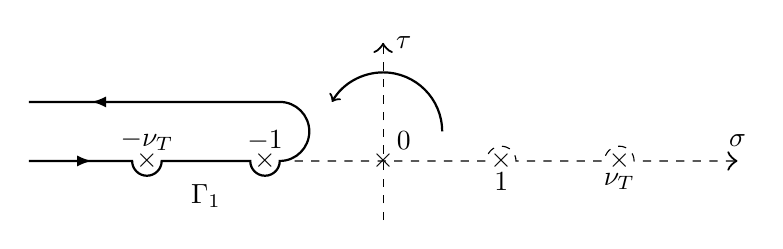
\begin{tikzpicture}[scale=0.75]
\node at (0,0) {$\times$};
\node at (0.35,0.35) {$0$};
\node at (2,0) {$\times$}; % Pole
\node at (4,0) {$\times$}; %pole
\node at (2,-0.35) {$1$};
\node at (4,-0.35) {$\nu_T$};

\node at (-2,0) {$\times$};
\node at (-4,0) {$\times$};
\node at (-2,0.35) {$-1$}; %pole
\node at (-4,0.35) {$-\nu_T$}; %pole
\node at (-3,-0.6) {$\Gamma_1$};

\node at (6,0.35) {$\sigma$};
\node at (0.35,2) {$\tau$};

\draw[dashed, decoration={markings,
 mark=at position 1.0 with {\arrow[scale=2]{>}}},
      postaction={decorate}] (-1.5,0) --(1.75,0) arc(180:0:0.25)--(3.75,0) arc(180:0:0.25)-- (6,0);
      
\draw[dashed, decoration={markings,
 mark=at position 1.0 with {\arrow[scale=2]{>}}},
      postaction={decorate}] (0,-1) -- (0,2);
      
\draw[ thick, ->] (1,0.5) arc (0:150:1);

\draw[thick, black, yshift=0pt,
decoration={ markings,  % This schema allows for fine-tuning the positions of arrows 
      mark=at position 0.1 with {\arrow{latex}},
      mark=at position 0.9 with {\arrow{latex}}},
      postaction={decorate}]
      (-6,0) -- (-4.25,0)  arc (-180:0:0.25) -- (-2.25,0)  arc (-180:0:0.25) -- (-1.75,0) arc(-90:90:0.5)  -- (-6,1);
\end{tikzpicture}
\caption{Contour $\Gamma_1$ in the complex plane $\xi=\sigma+i\tau$. The curved arrow indicates the contour deformation from $\Gamma_0$ to $\Gamma_1$}
\label{gamma1}
\end{figure}

Croisille and Lebeau \cite{CroisilleLebeau} proved that $D_p(z,\cdot)$ and $T_p(z,\cdot)$ belong to a special class of functions $\mathcal{H}^2$ defined hereafter

%\begin{mydef}
%\label{defHpl}
%$H^+$ is the space of functions f which are analytical in $\{z \in \mathbb{C}, \; \mbox{Im} z <0\}$  and verify :
%\begin{equation}
%\underset{c>0}{sup} \int_{-\infty}^{+\infty} |f(x-ic)|^2\,dx<+\infty
%\end{equation}
%\end{mydef}
%\begin{mydef}
%\label{defH}
%$\mathcal{H}$ is the space of the functions f analytical in $\mathbb{C}\backslash \rbrack -\infty,-1\rbrack$ such that $\forall \epsilon \in \rbrack0,\pi \lbrack, f(e^{i\epsilon} \cdot)\in H^+$.
%\end{mydef}

%Afin d'énoncer la nature des décompositions recherchées pour les fonctions spectrales, on définit tout d'abord un ensemble $Z^j(\cdot,\cdot)$. On commence par poser
%\begin{equation}
%Z_0^1=\{\nu_{\alpha}\cos \theta_{inc} \} \hspace{3em} Z_0^2=\{\nu_{\alpha} \cos(\varphi-\theta_{inc}) \}
%\end{equation}
%Les ensembles suivants sont définis par récurrence sur $l \geq 0$ :
%\begin{eqnarray}
%\left\{
%\begin{array}{l}
%Z^1_{l+1} =T_L(Z_l^2 \cap \Omega_L) \cup T_T(Z_l^2 \cap \Omega_T) \\
%Z^2_{l+1} =T_L(Z_l^1 \cap \Omega_L) \cup T_T(Z_l^2 \cap \Omega_T)
%\end{array}
%\right.
%\end{eqnarray}
%et enfin:
%\begin{equation}
%Z^j(\nu_{\alpha}\cos \theta_{inc},\nu_{\alpha}\cos(\varphi-\theta_{inc}))=\bigcup_{l\geq 0} Z^j_l(\nu_{\alpha}\cos \theta_{inc},\nu_{\alpha}\cos(\varphi-\theta_{inc})) \hspace{2em} j=1,2
%\end{equation}
%On admet l'hypothèse $(H)$ suivante :
%\begin{equation*}
%(H) \hspace{3em}  \{ \nu_L, \nu_T, \nu_R \} \cap Z^j(\nu_{\alpha}\cos \theta_{inc},\nu_{\alpha}\cos(\varphi-\theta_{inc})) = \emptyset, \hspace{3em} j=1,2
%\end{equation*}
%
%Il a été démontré par Kamotski et Lebeau \cite{Lebeau2} que, si l'hypothèse $(H)$ est vérifiée, alors les focntions spectrales peuvent se décomposer de la façon suivante :
%\begin{equation}
%\Sigma_j(\xi)=y_j(\xi)+X_j(\xi)
%\end{equation}
%avec $y_j$ singulière et $X_j$ régulière. 
%\paragraph{}
%Plus précisément, la fonctions $y_j$ est méromorphe et ses pôles sont dans $Z^j(Z^1_0,Z^2_0)$  et $X_j \in \mathcal{H}$ tel que ses valeurs limites $X_j(\xi-i0),\; \xi \in\mathbb{R}$ soient analytiques pour $\xi \notin \{-\nu_R,-\nu_T\} \cup Z^j(-\nu_L,-\nu_L)$.
%
%Nous allons maintenant voir comment calculer la partie singulière puis la partie régulière de cette décomposition.
%
%\subsubsection{Expression analytique des pôles et résidus des fonctions spectrales}
%\label{decomp}

Let us now extract all the poles and corresponding residues from the spectral functions, using system \eqref{equationsintegrales}. We begin by defining $X'_j$ by :
\begin{equation}
\Sigma_j(\xi)= \frac{V_j^{(0)}}{\xi-Z^{(0)}_j}+X'_j(\xi), \, \, \, j=1,2,
\label{firstep}
\end{equation}
where $V_j^{(0)}$ is unknown and $Z_1^{(0)}=\nu_{\alpha} \cos \theta_{inc}, \, Z_2^{(0)}=\nu_{\alpha} \cos(\varphi-\theta_{inc})$. Substituting \eqref{firstep} into \eqref{equationsintegrales} and applying formula \eqref{GaussDM} yields :
\begin{equation}
\left\{
\begin{matrix}
\textbf{DM}(X'_1)+\textbf{TM}(X'_2)+\textbf{TM}(\frac{V_2^{(0)}}{\xi-Z_2^{(0)}})=\frac{W^1}{\xi-Z_1^{(1)}}-\frac{\textbf{dm}(Z_1^{(0)}).V_1^{(0)}}{\xi-Z_1^{(0)}}-D_p(Z_1^{(0)},\xi).V_1^{(1)}\\
\textbf{TM}(X'_1)+\textbf{DM}(X'_2)+\textbf{TM}(\frac{V_1^{(0)}}{\xi-Z_1^{(0)}})=\frac{W^2}{\xi-Z_2^{(0)}}-\frac{\textbf{dm}(Z_2^{(0)}).V_2^{(0)}}{\xi-Z_2^{(0)}}-D_p(Z_2^{(0)},\xi).V_2^{(0)}
\end{matrix}
\right.
\end{equation}
In order to only have regular terms on the right-hand side of this system, we chose:
\begin{equation}
V_j^{(0)}=\textbf{dm}^{-1}(Z_j^{(0)}).W^j
\end{equation}
We have $\mbox{det}(\textbf{dm}(z) )\neq 0$ as long as $z\neq \nu_R$. In the following, we will suppose that this is the case. Physically, this means that the incident wave is not a Rayleigh wave and neither are any of the waves reflected by the wedge faces. Furthermore, we suppose that the hypothesis $z \notin \{ \nu_L, \nu_T\}$ that has been made in \eqref{GaussDM} and \eqref{GaussTM} remains true for all the poles. This means that neither the incident, nor any of the reflected waves is an incoming grazing one. Kamotski \cite{KamotskiCrit} proves existence and uniqueness of the solution in the case where this is not true.
%We now have :
%\begin{equation}
%\left\{
%\begin{matrix}
%\textbf{DM}(X'_1)+\textbf{TM}(X'_2)+\textbf{TM}(\frac{V_2^{(0)}}{\xi-Z_2^{(0)}})=-D_p(Z_1^{(0)},\xi).V_1^{(1)}\\
%\textbf{TM}(X'_1)+\textbf{DM}(X'_2)+\textbf{TM}(\frac{V_1^{(0)}}{\xi-Z_1^{(0)}})=-D_p(Z_2^{(0)},\xi).V_2^{(0)}
%\end{matrix}
%\right.
%\label{mille}
%\end{equation}

Applying \eqref{GaussTM}, two new poles appear :
\begin{equation}
Z^{(1)}_{j,L}=T_L(Z_j^{(0)}) \,\;\mbox{ et }\,\; Z^{(1)}_{j,T}=T_T(Z_j^{(0)})
\end{equation}
This leads to the definition of $X''_j$:
\begin{equation}
X'_j=X''_j+\frac{V_{j,L}^{(1)}}{\xi-Z_{j,L}^{(1)}}+\frac{V_{j,T}^{(1)}}{\xi-Z_{j,T}^{(1)}},
\end{equation}
where $V_{j,L}^{(1)}$ and $V_{j,T}^{(1)}$ are unknown vectors. Once again, we substitute this into the system and apply (\ref{GaussDM}). 
% Once again, we substitute this into (\ref{mille}) and apply (\ref{GaussDM}). 
Residues $V_{j,*}^{(1)}$ are chosen so as to only have regular terms on the left-hand side of the system:
\begin{equation}
V_{j,*}^{(1)}=-\textbf{dm}^{-1}(T_*(Z_{3-j}^{(0)})).\textbf{tm}_*(Z_{3-j}^{(0)}).V_{3-j}^{(0)}\mathbf{1}_{\Omega_*}(Z_{3-j}^{(0)})
\end{equation}
These steps are repeated recursively as long as the poles $Z_{j,L}^{(k)} \in \Omega_L^+$ and $Z_{j,T}^{(k)} \in \Omega_T^+$. When this is the case, \eqref{GaussTM} can be applied, creating new poles in the right-hand side of the system. These new poles are then extracted from the spectral functions using \eqref{GaussDM}, and so on. In the end, we have, for $\mbox{Im}\, \xi <0$ :
\begin{gather}
\Sigma_j(\xi)=Y_j(\xi)+X_j(\xi) \label{decomp}\\
Y_j(\xi)=\sum_k \sum_{*=L,T} \frac{V_{j,*}^{(k)}}{\xi-Z_{j,*}^{(k)}}
\label{yj},
\end{gather}
where
\begin{equation}
\begin{matrix}
Z_{1}^{(0)}=\nu_{\alpha} \cos \theta_{inc},  & Z_{2}^{(0)}=\nu_{\alpha} \cos(\varphi-\theta_{inc}) \\
Z_{j,L}^{(k+1)}= T_L(Z_{3-j,*}^{(k)}) &Z_{j,T}^{(k+1)}= T_T(Z_{3-j,*}^{(k)}) 
\end{matrix}
\end{equation}
and
\begin{equation}
\begin{matrix}
V_{j}^{(0)}=\textbf{dm}^{-1}(Z_{j}^{(0)}).W_j^{\alpha}\\
V_{j,L}^{(k+1)}=-\textbf{dm}^{-1}(Z_{j,*}^{(k+1)}).\textbf{tm}_L(Z_{3-j,*}^{(k)}).V_{3-j,*}^{(k)}.\textbf{1}_{\Omega_L}(Z_{3-j,*}^{(k)}) \\ 
V_{j,T}^{(k+1)}=-\textbf{dm}^{-1}(Z_{j,*}^{(k+1)}).\textbf{tm}_T(Z_{3-j,*}^{(k)}).V_{3-j,*}^{(k)}.\textbf{1}_{\Omega_T}(Z_{3-j,*}^{(k)}) 
\end{matrix}
\label{residus}
\end{equation}
The recursive procedure stops when the poles $Z_{j,*}^{(k)}$ exit $\Omega_L^+\cup\Omega_T^+$ (\textit{i.e.} when the translation operators $T_L$ and $T_T$ can no longer be applied to them). Croisille and Lebeau \cite{CroisilleLebeau} have shown that this defines a finite number of poles. Physically, this means that an incident ray exits the wedge after a finite number of reflections and mode conversions. We have thus extracted all the poles from the spectral functions and have computed them analytically, along with their corresponding residues. 

\subsection{Regular part}
\label{regpart}
The singular parts $Y_j$ of the spectral functions having been determined, two new functions $X_1$ and $X_2$ are defined by \eqref{decomp}. In the following, a numerical approximation method for $X_j$ is proposed. In order to do so, a system of functional equations solved by $X_1, X_2$ is derived by subtracting vector
\begin{equation}
\begin{pmatrix}
\textbf{DM}(Y_1)+\textbf{TM}(Y_2) \\
\textbf{TM}(Y_1)+\textbf{DM}(Y_2)
\end{pmatrix},
\end{equation}
where $Y_1$ and $Y_2$ are given by equations \eqref{yj} to \eqref{residus}, from both sides of (\ref{equationsintegrales}) :
\begin{equation}
\left\{ 
\begin{matrix}
\textbf{DM}(X_1)(\xi)+\textbf{TM}(X_2)(\xi)=u_1(\xi)\\
\textbf{TM}(X_1)(\xi)+\textbf{DM}(X_2)(\xi)=u_2(\xi)
\end{matrix}
\right.,
\label{regparteqn}
\end{equation}
with, for $j=1,2$
\begin{equation}
u_j(\xi)=-\sum_k \sum_{*=L,T} \left[ D_p(Z_{j,*}^{(k)},\xi).V_{j,*}^{(k)}+T_p(Z_{3-j,*}^{(k)},\xi).V_{3-j,*}^{(k)}\right]
\label{scndmembre}
\end{equation}
Croisille and Lebeau \cite{CroisilleLebeau} have shown that this system has a unique solution $(X_1,X_2)$ in $\mathcal{H}^2$ (defined in Def.\ref{defH}). In the sequel, a numerical approximation of the regular parts $X_j$ will be computed using a Galerkin collocation method.

The functional space $\mathcal{H}$ is approached by a finite-dimension space generated by the basis functions $\varphi_k$:
\begin{equation}
\varphi_k(\xi)= \sqrt{\frac{a_k}{\pi}} \frac{1}{\xi+a_k} \; \; (a_k)_{1 \leq k \leq N} \in (\lbrack 1, + \infty \lbrack)^N
\end{equation}
In this space, functions $X_j$ are approximated by
\begin{equation}
X_j(\xi) \approx \sum_{k=1}^N \tilde{X}_j^k \varphi_k(\xi), \; \tilde{X}_j^k \in \mathbb{C}^2 \;, j=1,2
\label{Xj}
\end{equation}
Substituting this approximation into \eqref{regparteqn} and applying 
%\begin{equation}
%\left\{
%\begin{matrix}
%\sum_{k=1}^N \tilde{X}_1^k \int_{\Gamma_0} \textbf{DM}(\xi,\zeta) \varphi_k(\zeta) \, d \zeta +\tilde{X}_2^k \int_{\Gamma_0} \textbf{TM}(\xi,\zeta) \varphi_k(\zeta) \, d \zeta \approx u_1(\xi) \\
%~\\
%\sum_{k=1}^N \tilde{X}_1^k \int_{\Gamma_0} \textbf{TM}(\xi,\zeta) \varphi_k(\zeta) \, d \zeta +\tilde{X}_2^k \int_{\Gamma_0} \textbf{DM}(\xi,\zeta) \varphi_k(\zeta) \, d \zeta \approx u_2(\xi)
%\end{matrix}
%\right.
%\end{equation}
variable change $\zeta=iy$ to this system before evaluating it at points $\xi=b_1,...,b_N$ leads to the following linear system of equations :
\begin{equation}
\left\{
\begin{matrix}
\sum_{k=1}^N \tilde{X}_1^k \int_{-\infty}^{+\infty} \textbf{DM}(b_1,iy)e_{a_k}(y) \, dy + \tilde{X}_2^k \int_{-\infty}^{+\infty} \textbf{TM}(b_1,iy)e_{a_k}(y) \, dy=u_1(b_1) \\
\vdots\\
\sum_{k=1}^N \tilde{X}_1^k \int_{-\infty}^{+\infty} \textbf{TM}(b_N,iy)e_{a_k}(y) \, dy + \tilde{X}_2^k \int_{-\infty}^{+\infty} \textbf{DM}(b_N,iy)e_{a_k}(y) \, dy=u_2(b_N)
\end{matrix}
\right.,
\label{linsys}
\end{equation}
where
\begin{equation}
e_{a_k}(y)=\sqrt{\frac{a_k}{\pi}} \frac{1}{y-ia_k} , \, 1 \leq k \leq N
\end{equation}
This system can be expressed in terms of matrices
\begin{equation}
\begin{pmatrix}
\mathbb{D}&\mathbb{T}\\
\mathbb{T}&\mathbb{D}
\end{pmatrix}
\begin{pmatrix}
\mathbb{X}_1 \\
\mathbb{X}_2
\end{pmatrix}
=
\begin{pmatrix}
\mathbb{U}_1 \\
\mathbb{U}_2
\end{pmatrix}
\iff
\left\{
\begin{matrix}
(\mathbb{D}+\mathbb{T})(\mathbb{X}_1+\mathbb{X}_2)=\mathbb{U}_1+\mathbb{U}_2\\
(\mathbb{D}-\mathbb{T})(\mathbb{X}_1-\mathbb{X}_2)=\mathbb{U}_1-\mathbb{U}_2
\end{matrix}
\right.
\label{systmat}
\end{equation}
where, for $1\leq l,k \leq N$ :
%\begin{equation}
%\begin{split}
%\mathbb{D}_{lk}&=\int_{-\infty}^{+\infty} \textbf{DM}(b_l,iy)e_{a_k}(y) \, dy \\
%\mathbb{T}_{lk}&=\int_{-\infty}^{+\infty} \textbf{TM}(b_l,iy)e_{a_k}(y) \, dy
%\end{split}
%\label{intDT}
%\end{equation}
%and
%\begin{equation}
%\mathbb{X}_j=
%\begin{pmatrix}
%\tilde{X}_j^1\\
%\vdots \\
%\tilde{X}_j^N
%\end{pmatrix}
%\hspace{3em}
%\mathbb{U}_j=
%\begin{pmatrix}
%u_j(b_1)\\
%\vdots \\
%u_j(b_N)
%\end{pmatrix}
%\end{equation}
%The coefficients of the linear combination \eqref{Xj} are computed by solving system \eqref{linsys} numerically. To do so, the coefficients of the system are computed analytically.

%\subsubsection{Calcul des coefficients de la matrice $\mathbb{D}$}
%Let us now compute coefficients of the linear system. The first coefficients are
%Passons maintenant au calcul effectif des coefficients des matrices de ce système. On a pour commencer, en utilisant (\ref{defDM}) :
\begin{equation}
\begin{split}
\mathbb{D}_{lk}=\int_{-\infty}^{+\infty} \textbf{DM}(b_l,iy)e_{a_k}(y) \, dy &=\frac{1}{2i\pi} \int_{-\infty}^{+\infty} \frac{\mathbf{dm}}{b_l-iy} 
%\begin{pmatrix}
%-1&A(iy) \\
%B(iy)&-1
%\end{pmatrix}
\sqrt{\frac{a_k}{\pi}}\frac{1}{y-ia_k} \, dy \\
&=- \frac{\sqrt{a_k}}{2\pi \sqrt{\pi}}
\begin{pmatrix}
\mathcal{D}_1(a_k,b_l) & \mathcal{D}_2(a_k,b_l) \\
\mathcal{D}_3(a_k,b_l) &\mathcal{D}_1(a_k,b_l)
\end{pmatrix}=\frac{\sqrt{a_k}}{2\pi \sqrt{\pi}}\mathbb{D}(a_k,b_l)
\end{split}
\label{Dab}
\end{equation}
%Using \eqref{defDM}, we can define :
%\begin{equation}
%\mathcal{D}_1(a,b)=\int_{-\infty}^{+\infty} \frac{dy}{(y+ib)(y-ia)} 
%\end{equation}
%\begin{equation}
%\mathcal{D}_2(a,b)=\int_{-\infty}^{+\infty} \frac{-iy(1-2\mu \zeta_L(iy) \zeta_T(iy)+2\mu y^2)}{(y+ib)(y-ia)\zeta_T(iy)} \,dy 
%\end{equation}
%\begin{equation}
%\mathcal{D}_3(a,b)=\int_{-\infty}^{+\infty} \frac{iy(1-2\mu \zeta_L(iy) \zeta_T(iy)+2\mu y^2)}{(y+ib)(y-ia)\zeta_L(iy)} \,dy
%\end{equation}
The explicit expressions of operators $\mathcal{D}_i, 1\leq i\leq3$ and their values are computed in \ref{compD}.
The other coefficients of the system are, for $1\leq l,k \leq N$
\begin{equation}
\begin{split}
\mathbb{T}_{lk}=\int_{-\infty}^{+\infty} \textbf{TM}(b_l,iy)e_{a_k}(y) \, dy 
&=\frac{1}{2i\pi} \int_{-\infty}^{+\infty} \sum_{*=L,T} \frac{\textbf{tm}_* (iy, \mbox{sgn} \sin \varphi)}{b_l-T_*(iy)} \sqrt{\frac{a_k}{\pi}}\frac{1}{y-ia_k}\,dy \\
&=\frac{1}{2i\pi}\sqrt{\frac{a_k}{\pi}}\sum_{*=L,T} \int_{-\infty}^{+\infty} \frac{\textbf{tm}_*(iy,\epsilon)}{\lbrack b_l-(iy \cos \varphi +  \zeta_*(iy)| \sin \varphi|)\rbrack(y-ia_k)} \, dy,
\end{split}
\end{equation}
where $\epsilon= \mbox{sgn}( \sin \varphi)$. Let us define
\begin{equation}
\mathbb{T}_{lk}=\frac{\mu}{2i\pi}\sqrt{\frac{a_k}{\pi}}
\begin{pmatrix}
\mathcal{T}_1^L(a_k,b_l)+ \mathcal{T}_1^T(a_k,b_l)  &  \mathcal{T}_2^L(a_k,b_l) + \mathcal{T}_2^T(a_k,b_l)  \\
 \mathcal{T}_3^L(a_k,b_l)+ \mathcal{T}_3^T(a_k,b_l) &\mathcal{T}_4^L(a_k,b_l)+ \mathcal{T}_4^T(a_k,b_l)
\end{pmatrix}
=\frac{1}{2i\pi}\sqrt{\frac{a_k}{\pi}}\mathbb{T}(a_k,b_l)
\label{Tab}
\end{equation}
The explicit expressions of operators $\mathcal{T}_i^*, 1\leq i\leq4, *=L,T$ and their values are computed in \ref{compT}.

Finally, for $j=1,2$ :
\begin{equation}
\mathbb{X}_j=\begin{pmatrix}
\tilde{X}^1_j \\
\vdots \\
\tilde{X}^1_j
\end{pmatrix}, \,
\tilde{X}^k_j \in \mathbb{C}^2; \hspace{2em}
\mathbb{U}_j=\begin{pmatrix}
u_j(b_1)\\
\vdots \\
u_j(b_N)
\end{pmatrix}, \,
u_j(b_k) \in \mathbb{C}^2
\end{equation}
where $u_j(\xi)$ is given by \eqref{scndmembre}. Applying variable change $\zeta=iy$ to the definition of $D_p$ given by 
\eqref{GaussDM} and substituting \eqref{Dab} in the result gives
\begin{equation}
D_p(z,\xi)=\frac{1}{2\pi}\mathbb{D}(-z,\xi)-\frac{\textbf{dm}(z)}{\xi-z}
\label{Dpscm}
\end{equation}
Similarly, applying variable change $\zeta=iy$ to \eqref{GaussTM} and substituting \eqref{Tab} in the result yields
\begin{equation}
T_p(z,\xi)=\frac{1}{2i\pi}\mathbb{T}(-z,\xi)- \sum_{*=L,T}\frac{\textbf{tm}_*(z,\epsilon)}{b-T_*(z)}\textbf{1}_{\Omega_*}(z)
\label{Tpscm}
\end{equation}
Equations \eqref{Dpscm} and \eqref{Tpscm} are substituted into \eqref{scndmembre}. By construction, the singular terms cancel each other and the remaining terms are :
\begin{equation}
u_j(\xi)=-\frac{1}{2i\pi}\sum_{k}\sum_{*=L,T}\left(i\mathbb{D}(-Z_{j,*}^{(k)},\xi).V_{j,*}^{(k)}+\mathbb{T}(-Z_{3-j,*}^{(k)},\xi).V_{3-j,*}^{(k)} \right) +\frac{W_j^{\alpha}}{\xi-Z_j^{(0)}}
\label{uDT}
\end{equation}

Using these results, the linear system \eqref{systmat} can be implemented and solved numerically thanks to the C++ library Eigen, and an evaluation of the regular part of the spectral functions is obtained. However, for values of $\xi$ lying in certain parts of the complex plane, this evaluation is not sufficiently accurate. The technique used to solve this problem is called the propagation of the solution.

\subsection{Propagation of the solution}
\label{C3:propag}
The method described hereafter is used to ``propagate''  the accuracy of the solution to \eqref{regparteqn} to the whole complex plane. This is done by determining a new system of recursive equations solved by $X_1, X_2$ in which the regular part $X_j$ is expressed using the value of $X_1, X_2$ in a domain where the numerical approximation is valid.

By deforming $\Gamma_0$ into $\Gamma_2$, represented in Fig. \ref{contour2}, the half-plane Im $\xi<0$  is entirely crossed. Note that the branch points $\pm \nu_*, *=L,T$ are not crossed during this deformation, indicated by the curved arrow in Fig.~\ref{contour2}. The contribution of poles $\zeta=\xi, \, \rm Im \xi<0$, is given by Cauchy's integral formula :
\begin{equation}
\int_{\Gamma_0} \textbf{DM}(\xi,\zeta)X_j(\zeta)\, d\zeta = \int_{\Gamma_2}  \textbf{DM}(\xi,\zeta)X_j(\zeta)\, d\zeta + \textbf{dm}(\xi).X_j(\xi)
\label{DM2}
\end{equation}
\begin{figure}[h]
	\centering
	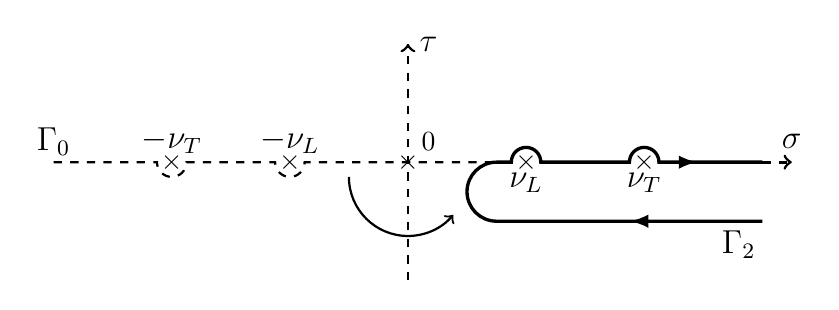
\begin{tikzpicture}[scale=0.75]
	\node at (0,0) {$\times$};
	\node at (0.35,0.35) {$0$};
	\node at (2,0) {$\times$}; 
	\node at (2,-0.35) {\large $\nu_L$};
	\node at (4,0) {$\times$};
	\node at (4,-0.35) {\large $\nu_T$};
	\node at (-2,0) {$\times$};
	\node at (-2,0.35) {\large $-\nu_L$};
	\node at (-4,0) {$\times$};
	\node at (-4,0.35) {\large $-\nu_T$};
	\node at (5.6,-1.4) {\large $\Gamma_2$};
	\node at (0.35,2) {\large $\tau$};
	\node at (6.5,0.35) {\large $\sigma$};
	\node at (-6,0.35) {\large $\Gamma_0$};
	
	\draw[very thick, black,yshift=0pt,
	decoration={ markings,  % This schema allows for fine-tuning the positions of arrows 
		mark=at position 0.2 with {\arrow{latex}},
		mark=at position 0.9 with {\arrow{latex}}},
	postaction={decorate}]
	(6,-1) -- (1.5,-1)  arc (90:-90:-0.5)  -- (1.5,0) -- (1.75,0) arc (180:0:0.25) -- (3.75,0) arc (180:0:0.25) -- (6,0);
	
	\draw[dashed, line width = 0.8pt,yshift=0pt]
	(-6,0) -- (-4.25,0) arc (-180:0:0.25) -- (-2.25,0)  arc (-180:0:0.25)  -- (1.5,0);
	
	\draw[dashed, line width = 1pt,yshift=0pt,
	decoration={ markings,  mark=at position 1 with {\arrow{>}}},
	postaction={decorate}] (0,-2)--(0,2);
	
	\draw[dashed, line width = 1pt,yshift=0pt,
	decoration={ markings,  mark=at position 1 with {\arrow{>}}},
	postaction={decorate}] (6,0)--(6.5,0);
	
	\draw[ thick, ->] (-1,-0.25) arc (180:320:1);
	
	\end{tikzpicture}
	\caption{Integration contour $\Gamma_2$ in the complex place $\xi=\sigma+i\tau$. The curved arrow indicates the contour deformation from $\Gamma_0$ to $\Gamma_2$.}
	\label{contour2}
\end{figure}

It is now necessary to define the inverse transformation operator $T_*^{-1}, *=L,T$ :
\begin{equation}
T_*^{-1}(\xi=\nu_*\cos\theta)=\xi \cos \phiti-\zeta_*(\xi)\sin\phiti=\nu_*\cos(\theta-\tilde{\varphi}).
\end{equation}
In order for the cosine in this translation operator to be well defined, it is necessary to impose
\begin{equation}
\xi \in \Omega_*^-=\{\xi=\nu_*\cos\theta, \, \, \, \tilde{\varphi}\leq \mbox{Re}\theta\leq\pi, \, \, \, \mbox{Im}\xi< 0\},
\end{equation}
where $\Omega_*^-$ is represented in Fig.~\ref{dOmegamoins}. By deforming contour $\Gamma_0$ into contour $\partial \Omega_*^-$ (also represented in Fig.~\ref{dOmegamoins}), domain $\Omega_*^-$ is crossed. The contribution of poles $\zeta=T_*^{-1}(\xi)$, when $\xi\in\Omega_*^-$  is taken into account using Cauchy's integral formula :
\begin{equation}
\int_{\Gamma_0} \textbf{TM}(\xi,\zeta)X_j(\zeta)\, d\zeta = \int_{\partial \Omega_*^-}  \textbf{TM}(\xi,\zeta)X_j(\zeta)\, d\zeta+\sum_{*=L,T} \mathbf{M}_*(\xi).X_j(T^{-1}_*(\xi))\textbf{1}_{\Omega_*^-}(\xi),
\label{TM2}
\end{equation}
where $\textbf{1}_{\Omega_*^-}(\xi)=1$ when $\xi \in \Omega_*^-$ and $0$ elsewhere and
\begin{equation}
\mathbf{M}_*(\xi=\nu_*\cos\theta)=-\frac{\sin(\theta-\tilde{\varphi})}{\sin\theta} \textbf{tm}_*(T_*^{-1}(\xi))
\end{equation}

\begin{figure}[ht]%
\begin{center}
	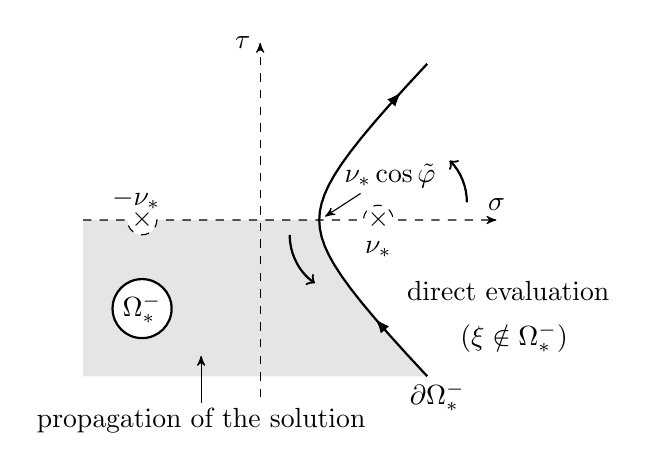
\begin{tikzpicture}[scale=0.75]
	% Filling Omega_*^-
	\fill [color=gray!20]
	(-1,0)
	-- plot [domain= 0:1.7] ({cosh(\x)},{-sinh(\x)})
	-- (-3,0)
	-- cycle;
	
	\fill [color=gray!20]
	({cosh(1.7)},{-sinh(1.7)})
	-- plot [domain= 0:-3] ({\x},{-sinh(1.7)})
	-- (-3,0)
	-- cycle;
	
	\fill[color=white] (-2,0) circle (0.25);
	
	\draw[dashed, ->,>=stealth'] (-3,0)  -- (-2.25,0) arc(-180:0:0.25)--(1.75,0) arc (180:0:0.25)--(4,0) node[above]{$\sigma$};
	\draw[dashed, ->,>=stealth'](0,-3)--(0,3) node[left]{$\tau$};
	\node at (2,0) { $\times$}; 
	\node at (2,-0.5) {$\nu_*$};
	\node at (-2,0) { $\times$};
	\node at (-2.1,0.35) {$-\nu_*$};
	
	% Hyperbola (contour  partial_Omega_0 )
	\draw[black, thick,decoration={ markings,  % This schema allows for fine-tuning the positions of arrows 
		mark=at position 0.2 with {\arrow{latex}},
		mark=at position 0.9 with {\arrow{latex}}},
	postaction={decorate}][domain=-1.7:1.7] plot({cosh(\x)}, {sinh(\x)});
	
	\node at (3,-3) {$\partial \Omega_*^-$};
	\draw[thin, ->,>=stealth'](1.7,0.45) -- (1.1, 0.06);
	\node at (2.2, 0.75) { $\nu_*\cos \tilde{\varphi}$};
	
	% Omega_0
	\draw[->,>=stealth'] (-1,-3.1) -- (-1,-2.3);
	\node at (-1,-3.4) {propagation of the solution};
	\node at (4.2,-1.2) {direct evaluation};
    \node at (4.3,-2) { $(\xi \notin \Omega_*^-)$};

	% Espace Omega_0
\fill [color=white] (-2,-1.5) circle (0.5);
\draw[thick] (-2,-1.5) circle (0.5);
\node at (-2,-1.5) {$\Omega_*^-$};

\draw[thick, ->] (0.5,-0.25) arc (180:235:1);
\draw[thick, ->] (3.5,0.3) arc (0:45:1); %ici c'est les fleches 
	
	\end{tikzpicture}
\end{center}
\caption{Domain $\Omega_*^-$ and contour $\partial \Omega_*^-$ in the complex plane $\xi=\sigma + i \tau$. The curved arrows indicate contour deformation from $\Gamma_0$ to $\partial \Omega_*^-$. }
\label{dOmegamoins}
\end{figure}
The recursive system of functional equations solved by the regular part is obtained by substituting \eqref{DM2} and \eqref{TM2} into \eqref{regparteqn}:
\begin{equation}
\left\{
\begin{matrix}
X_1(\xi) =g_1(\xi)-\textbf{dm}^{-1}(\xi).\underset{*=L,T}{\sum} \mathbf{M}_*(\xi).X_2(T_*^{-1}(\xi))\textbf{1}_{\Omega_*^-}(\xi) \\
X_2(\xi) =g_2(\xi)-\textbf{dm}^{-1}(\xi).\underset{*=L,T}{\sum} \mathbf{M}_*(\xi).X_1(T_*^{-1}(\xi))\textbf{1}_{\Omega_*^-}(\xi)
\end{matrix}
\right.,
\label{recur}
\end{equation}
where , for $j=1,2$
\begin{equation}
g_j(\xi)=\textbf{dm}^{-1}(\xi)\left( u_j(\xi)- \int_{\Gamma_2}  \textbf{DM}(\xi,\zeta)X_j(\zeta)\, d\zeta- \int_{\partial \Omega_*^-}  \textbf{TM}(\xi,\zeta)X_{3-j}(\zeta)\, d\zeta \right) 
\label{g1g2}
\end{equation}

This new recursive system is used to evaluate the spectral functions in the domain $W=\{ \mbox{Im}(\xi)<0, \xi \notin \partial \Omega_*^- \}$. To do so, functions $g_j$ must be evaluated numerically.

Each of the integrals appearing in the definition of $g_j$ are evaluated separately using the approximation of the regular part \eqref{Xj} for the computation of terms $X_j(\zeta)$ and $X_{3-j}(\zeta)$. 

Substituting \eqref{Dab} into \eqref{DM2} yields :
\begin{equation}
\int_{\Gamma_2}\textbf{DM}(\xi,\zeta)\varphi_k(\zeta) \, d\zeta = \int_{\Gamma_0}\textbf{DM}(\xi,\zeta)\varphi_k(\zeta)\, d\zeta -\textbf{dm}(\xi).\varphi_k(\xi)=\frac{1}{2\pi}\sqrt{\frac{a_k}{\pi}} \mathbb{D}(a_k,\xi)-\textbf{dm}(\xi).\varphi_k(\xi) 
\label{NDreg}
\end{equation}
and substituting \eqref{Tab} into \eqref{TM2} yields:
\begin{equation}
\begin{split}
\int_{\partial \Omega_*^-}  \textbf{TM}(\xi,\zeta)\varphi_k(\zeta)\, d\zeta&=\int_{\Gamma_0} \textbf{TM}(\xi,\zeta)\varphi_k(\zeta)\, d\zeta  -\sum_{*=L,T} \mathbf{M}_*(\xi).\varphi_k(T^{-1}_*(\xi)) \\
= &\frac{1}{2i\pi} \sqrt{\frac{a_k}{\pi}} \mathbb{T}(a_k,\xi)- \sum_{*=L,T}\mathbf{M}_*(\xi).\varphi_k(T^{-1}_*(\xi))\textbf{1}_{\Omega_*^-}(\xi)
\end{split}
\label{NTreg}
\end{equation}
Finally, \eqref{NDreg} and \eqref{NTreg} can be injected into \eqref{g1g2} :
\begin{equation}
\textbf{dm}(\xi).g_j(\xi)=u_j(\xi)-\sum_{k=1}^N \sqrt{\frac{a_k}{\pi}}\left( \mathbb{ND}(a_k,\xi).\tilde{X}_j^k+\mathbb{NT}(a_k,\xi).\tilde{X}_{3-j}^k \right) ,
\label{gjfinal}
\end{equation}
where
\begin{equation}
\mathbb{ND}(a,b)=\frac{1}{2\pi}\mathbb{D}(a,b)-\frac{\textbf{dm}(b)}{a+b}
\label{defND}
\end{equation}
and
\begin{equation}
\mathbb{NT}(a,b)=\frac{1}{2i\pi}\mathbb{T}(a,b)-\sum_{*=L,T}\frac{\mathbf{M}_*(b)}{T^{-1}_*(b)+a} .
\end{equation}

In system \eqref{recur}, the value of the regular part of the spectral function in domain $\Omega_*^-$, visible Fig.~\ref{dOmegamoins}, is expressed using its value in the domain $\xi \notin \Omega_*^-$, where the numerical approximation \eqref{Xj} is valid. To do so, functions $g_j,\, j=1,2$ are evaluated using \eqref{gjfinal}. The accuracy of the numerical evaluation in domain $\xi \notin \Omega_*^-$ is therefore propagated to domain $\Omega_*^-$. 

This concludes the semi-analytical computation of the spectral functions. Numerical comparisons with other codes are presented in the following.


\section{Numerical validation}
The longitudinal and transversal diffraction coefficients are computed using \eqref{DL} and \eqref{DT}. The spectral functions are evaluated in $\xi=\nu_*\cos\theta -i10^{-8}$ (a small negative imaginary part is added to ensure that the recursive equations \eqref{recur} are valid). This is achieved by, first, computing the poles and residues of the spectral functions analytically using the recursive algorithm described in subsection \ref{singpart}. Then, the regular parts of the spectral functions are approached numerically by solving \eqref{regparteqn} thanks to the Galerkin collocation method described in subsection \ref{regpart}, where the Galerkin parameters are set to:
\begin{equation}
a_k=1.0001+0.05e^{k\frac{\log 10}{4}}-1, \hspace{3em} b_k=a_k-0.1i, \hspace{3em} 1\leq k\leq20
\end{equation}
Finally, the solution is rendered accurate in the entire complex domain by applying the recursive procedure called the propagation of the solution described in subsection \ref{C3:propag}.

Following these steps, the diffraction coefficients have been computed every $0.2 ^o$ for a steel wedge in which $c_L=5700 m.s^{-1}, c_T=3100 m.s^{-1}$. The results are presented hereafter.
\subsection{For $\varphi<\pi$}
For wedge angles $\varphi<\pi$, the \acrfull{lt} code of Gautesen and Fradkin \cite{GautesenFradkin}, based on the method briefly recalled in \ref{C1:lt} has been used to validate the results of the \acrfull{sf} method. 

Fig.~\ref{8055} shows the absolute value of the diffraction coefficients  with respect to the observation angle obtained for a wedge of angle $\varphi=80^o$ illuminated by a wave incident with an angle $\theta_{inc}=55^o$. The green line represents the diffraction coefficients obtained using only the singular parts $Y_j$ of the spectral functions. The dark blue line is the diffraction coefficient obtained using the \acrshort{lt} code and the red circles represent the result obtained using the \acrshort{sf} code. These two plots are perfectly overlapping. The singular part alone, however, is not sufficient to compute accurate coefficients. 

Fig.~\ref{16040} shows the absolute value of the diffraction coefficients with respect to the observation angle obtained for a wedge of angle $\varphi=160^o$ illuminated by a wave incident with an angle $\theta_{inc}=40^o$. The light blue line represents the diffraction coefficients obtained without applying the ``propagation of the solution'' technique for the \acrshort{sf} code. The dark blue line is the diffraction coefficient obtained using the \acrshort{lt} code and the red circles represent the result obtained using the \acrshort{sf} code, including the ``propagation of the solution'' technique. These two plots are perfectly overlapping. Furthermore, the ``propagation of the solution'' technique is necessary in order to avoid coefficients which diverge near the wedge faces. 

\begin{figure}%[h!]
\centering
    \begin{subfigure}[b]{0.44\textwidth}
        \includegraphics[width=\textwidth]{images/chapter3/Figure8a.pdf}
        \caption{Diffracted and incident L waves}
    \end{subfigure}  
    \begin{subfigure}[b]{0.44\textwidth}
        \includegraphics[width=\textwidth]{images/chapter3/Figure8b.pdf}
        \caption{Diffracted T wave and incident L wave}
     \end{subfigure} \\   
     \begin{subfigure}[b]{0.44\textwidth}
        \includegraphics[width=\textwidth]{images/chapter3/Figure8c.pdf}
        \caption{Diffracted L wave and incident T wave}
    \end{subfigure}
    \begin{subfigure}[b]{0.44\textwidth}
        \includegraphics[width=\textwidth]{images/chapter3/Figure8d.pdf}
        \caption{Diffracted and incident T waves}
     \end{subfigure}
     \caption{Diffraction coefficients for $\varphi=80^o, \theta_{inc}=55^o$}
     \label{8055}
\end{figure}

\begin{figure}
\centering
    \begin{subfigure}[b]{0.44\textwidth}
        \includegraphics[width=\textwidth]{images/chapter3/Figure9a.pdf}
        \caption{Diffracted and incident L waves}
    \end{subfigure}  
    \begin{subfigure}[b]{0.44\textwidth}
        \includegraphics[width=\textwidth]{images/chapter3/Figure9b.pdf}
        \caption{Diffracted T wave and incident L wave}
     \end{subfigure} \\   
     \begin{subfigure}[b]{0.44\textwidth}
        \includegraphics[width=\textwidth]{images/chapter3/Figure9c.pdf}
        \caption{Diffracted L wave and incident T wave}
    \end{subfigure}
    \begin{subfigure}[b]{0.44\textwidth}
        \includegraphics[width=\textwidth]{images/chapter3/Figure9d.pdf}
        \caption{Diffracted and incident T waves}
     \end{subfigure}
     \caption{Diffraction coefficients for $\varphi=160^o, \theta_{inc}=40^o$}
     \label{16040}
\end{figure}

For all of the tested configurations (different wedge and incidence angles), the results are conclusive. The results using the spectral functions method are extremely close to those obtained using the \acrshort{lt} code, which has been validated both numerically and experimentally \cite{GautesenFradkin, ChapmanBurch}. This constitutes a satisfying validation for wedge angles $\varphi \leq \pi$. Some additional numerical comparisons have been made in the next section for the case of a wedge of angle $\varphi>\pi$.

\subsection{For $\varphi>\pi$}
For wedge angles $\varphi \geq \pi$, the existing \acrshort{lt} code can not be used. Therefore, the spectral finite elements code of Imperiale et al. developed for the commercial software CIVA \cite{imperiale_ut_2016, imperiale_ut_2017} has been used as a reference solution for numerical validation purposes. The scattered wave fronts have been computed using this \acrfull{fe} method and the diffraction coefficients are extracted from these. The frequency of the incident wave is set to $f=1,0$MHz. The \acrshort{fe} computation box is visible on the snapshots in Fig.~\ref{snap}. The mesh size is $h=0,0432 \rm mm$ and the simulation time step is set to verify the \acrfull{cfl} stability condition ($\delta t=1,40963 \mu s$). The boundaries of the \acrshort{fe} computation box which correspond to the wedge edges are set to be stress-free boundaries and the other boundaries of the domain are \acrfull{pml}, which are absorbing boundaries used to mimic an infinite propagation domain.

The \acrshort{fe} code computes the reflected and diffracted wave field in the time-domain. The incident wave is a pulse with a plane wavefront and the value of the diffracted wave field is extracted along the cylindrical diffracted wavefront as detailed in the following. To do so, a snapshot is taken at a time where the diffracted wavefronts are located inside the \acrshort{fe} box but the furthest possible from the edge, in order for the far-field approximation to be applicable, whilst minimizing interferences that may occur from non-physical waves reflected from the borders of the \acrshort{fe} computation domain. These snapshots are presented in Fig.~\ref{snap} for two different propagation times. 

Fig.~\ref{snapLL} shows the snapshot used in the case of an L wave incident with an angle $\theta_{inc}=135^o$. The cylindrical wavefronts of the L (dLW) and T (dTW) waves diffracted from the wedge edge are visible, as well as the reflected L (rLW) and T (rTW) waves on each face of the wedge. Finally, Rayleigh waves (RW) propagating along each face of the wedge interfere with the diffracted T wave at the vicinity of the wedge faces for the chosen propagation time. 
Similarly, fig.~\ref{snapTL} shows the snapshot simulated in the case of a T wave incident with an angle $\theta_{inc}=135^o$. Once again, the cylindrical wavefronts of the L (dLW) and T (dTW) waves diffracted from the wedge edge are visible. In this case, there is no mode conversion and only reflected T waves (rTW) appear. Rayleigh waves (RW) which interfere with the diffracted T wave are also visible in this case and head waves (HW) are emanated from each face at the medium's longitudinal critical angle (for a steel/void interface, this angle is $\theta_c \approx 57^o$  inside steel). Some models have recently been proposed to mimic some head waves for half-plane scatterers \cite{PTDdarmon, FradkinDarmon}.

In order to extract diffraction coefficients from the \acrshort{fe} wave field, formula \eqref{defcoeffdiff} is used. The diffraction coefficient is deduced from the \acrshort{fe} wave field by :
\begin{equation}
D_{\beta}^{\alpha}(\theta)=\frac{v^{diff}_{\beta}(r\cos\theta,r\sin\theta)}{v_{inc}^{\alpha}(r\cos\theta,r\sin\theta)}e^{i\nu_{\beta}r}\sqrt{\nu_{\beta}r}
\label{FEextract}
\end{equation}
For each of these snapshots, the distance $r$ from the edge to the wavefront of the considered (L or T) edge diffracted wave is computed using the wave velocity and the chosen propagation time, and the norm of the field $||v^{diff}_{\beta}||$ is extracted on the point of the \acrshort{fe} mesh which is closest to the wavefront for each observation angle $\theta$. The diffraction coefficient is finally computed using formula \eqref{FEextract}. The results are shown in Fig.~\ref{270135}.

\begin{figure}
\centering
    \begin{subfigure}[b]{0.44\textwidth}
        \includegraphics[width=\textwidth]{images/chapter3/Figure10a.pdf}
        \caption{Incident L wave, $t=5ms$.}
        \label{snapLL}
    \end{subfigure}  
    ~
     \begin{subfigure}[b]{0.44\textwidth}
        \includegraphics[width=\textwidth]{images/chapter3/Figure10b.pdf}
        \caption{Incident T wave, $t=6,5ms$. }
        \label{snapTL}
    \end{subfigure}
     \caption{Finite elements snapshots. Distances are given in millimeters. }
     \label{snap}
\end{figure}

\begin{figure}%[H]
\centering
    \begin{subfigure}[b]{0.44\textwidth}
        \includegraphics[width=\textwidth]{images/chapter3/Figure11a.pdf}
        \caption{Diffracted and incident L waves. $r=25,6 \rm mm$.}
        \label{DLL}
    \end{subfigure}  
    \begin{subfigure}[b]{0.44\textwidth}
        \includegraphics[width=\textwidth]{images/chapter3/Figure11b.pdf}
        \caption{Diffracted T wave and incident L wave. $r=13,9 \rm mm$.}
        \label{DLT}
     \end{subfigure}   
     \begin{subfigure}[b]{0.44\textwidth}
        \includegraphics[width=\textwidth]{images/chapter3/Figure11c.pdf}
        \caption{Diffracted L wave and incident T wave. $r=36,5 \rm mm$.}
        \label{DTL}
    \end{subfigure}
    \begin{subfigure}[b]{0.44\textwidth}
        \includegraphics[width=\textwidth]{images/chapter3/Figure11d.pdf}
        \caption{Diffracted and incident T waves. $r=19,8 \rm mm$.}
        \label{DTT}
     \end{subfigure}
     \caption{Diffraction coefficients for $\varphi=270^o, \theta_{inc}=135^o$}
     \label{270135}
\end{figure}

Fig.~\ref{270135} shows the absolute value of the diffraction coefficients, obtained for a wedge of angle $\varphi=270^o$ illuminated by a wave incident with an angle $\theta_{inc}=135^o$, plotted with respect to the observation angle. The blue line is the diffraction coefficient extracted from the finite elements wave front and the dashed red line is the result obtained from the \acrshort{sf} code. 

Overall, both lines overlap quite well, though some differences are observed. The most obvious difference between the plots is that the \acrshort{fe} diffraction coefficient always remains finite, whereas the \acrshort{sf} diffraction coefficient possesses poles (except for Fig.~\ref{DLT} where there are no reflected L waves). This is due to the fact that the \acrshort{sf} diffraction coefficient is a \acrshort{gtd}-like coefficient obtained from a far-field asymptotic evaluation \eqref{defcoeffdiff} and it diverges at shadow boundaries \cite{GTD,Audrey}. The \acrshort{fe} code notably computes the reflected waves as well as the diffracted waves in angular regions surrounding the reflected poles ; consequently, reflected waves give a contribution to the \acrshort{fe} diffraction coefficient. The contribution of these reflected plane waves to the \acrshort{fe} diffraction coefficient, computed using \eqref{FEextract}, grows with the distance $r$, since it contains the factor $\sqrt{\nu_{\beta}r}$ and the reflected plane waves have theoretically constant amplitudes. Interference between these plane reflected waves and the cylindrical diffracted waves explain the spikes that can be observed in the \acrshort{fe} diffraction coefficients, near the poles of the \acrshort{gtd} diffraction coefficients in Figs.~\ref{DLL}, \ref{DLT} and \ref{DTT}. Some uniform methods have been proposed to handle the divergence of \acrshort{gtd} diffraction coefficients and build a spatially uniform total field and some of them have been applied to elastodynamic half-plane scattering \cite{Audrey, Zernov, PTDdarmon}.

On Figs.~\ref{DLT} and \ref{DTT} for diffracted T waves, the \acrshort{fe} diffraction coefficient seems to have a slightly different behavior near the wedge edges than the \acrshort{sf} diffraction coefficients. Since this discrepancy is only visible in the T diffraction coefficient, it seems unlikely that it is due to the branch points at angles $\theta=0$ and $\theta=\varphi$ mentioned in section \ref{farfield}, as these branch points would affect both L and T diffracted waves. The observed discrepancy is more probably due to interference of the diffracted T wavefront with the Rayleigh waves observed on Figs.~\ref{snapLL} and \ref{snapTL}, which modifies the observed \acrshort{fe} field along the diffracted T wavefront.

Away from shadow boundaries (where the non-uniform \acrshort{sf} code diverges) and domain borders i.e. in regions where diffracted waves do not interfere with other waves and where the \acrshort{sf} asymptotic evaluation is theoretically valid, the \acrshort{fe} and \acrshort{sf} codes give very similar results. 

\section{Experimental validation}
The \acrshort{lt} code used to validate the \acrshort{sf} method for wedge angles lower than $\pi$ has been validated experimentally by Chapman et al. \cite{ChapmanBurch}. Their experimental set-up is thoroughly described in \cite{ChapmanBurch} and will only be summarized here. The results of their experimental measurements will be used to validate the \acrshort{sf} code experimentally.

\begin{figure}[h!]
\centering
\includegraphics[scale=0.8]{images/chapter3/wedge_schema.png}
\caption{(Reproduced from \cite{ChapmanBurch}) Front and Top view of the wedge inspected in pulse-echo configuration.}
\label{C3:wedge_schema}
\end{figure}

Two isotropic ferritic steel ($c_L=5900\,m.s^{-1}, \; c_T=3230\,m.s^{-1}$) cylindrical sectors of radius 150mm, thickness 100mm wedges and of angles $\varphi=80^o$ and $\varphi=100^o$ are inspected in pulse-echo configuration, meaning that the emitting transducer is also the receiving transducer. In terms of the diffraction coefficient, this means that the observation angle is equal to the incidence angle.

\begin{figure}[h!]
\centering
    \begin{subfigure}[b]{0.45\textwidth}
        \includegraphics[width=\textwidth]{images/chapter3/Retrodiff_D_80_LL.png}
        \caption{Incident and diffracted L wave, $\varphi=80^o$.}
        \label{C3:DLL80}
    \end{subfigure}
    \hfill  
    \begin{subfigure}[b]{0.45\textwidth}
        \includegraphics[width=\textwidth]{images/chapter3/Retrodiff_D_80_TT.png}
        \caption{Incident and diffracted T wave, $\varphi=80^o$.}
        \label{C3:DTT80}
     \end{subfigure} %\\  
%     \begin{subfigure}[b]{0.45\textwidth}
%        \includegraphics[width=\textwidth]{images/chapter3/Retrodiff_D_100_LL.png}
%        \caption{Incident and diffracted L wave, $\varphi=100^o$.}
%        \label{C3:DLL100}
%    \end{subfigure}
    \hfill
    \begin{subfigure}[b]{0.45\textwidth}
        \includegraphics[width=\textwidth]{images/chapter3/Retrodiff_D_100_TT.png}
        \caption{Incident and diffracted T wave, $\varphi=100^o$.}
        \label{C3:DTT100}
     \end{subfigure}
     \caption{Absolute value of the backscattering diffraction coefficients for wedges $\varphi=80^o$ and $\varphi=100^o$.}
     \label{C3:expcoeffs}
\end{figure}

The inspections have been done at frequencies 2MHz and 5MHz to check that the diffraction coefficients do not depend on the frequency.  The experimental set-up is shown in Fig.~\ref{C3:wedge_schema} and. Since the diffraction coefficients measured at both frequencies are identical, only the results obtained at 2MHz are presented here. Figs.~\ref{C3:expcoeffs} and \ref{C3:expcoeffsph} present the comparison between the backscattering coefficients computed using the \acrshort{lt} code, the coefficients computed using the \acrshort{sf} code and the values measured experimentally presented in \cite{ChapmanBurch}.

Figs.~\ref{C3:DLL80} and \ref{C3:DTT80} show the absolute values of the L and T backscattering diffraction coefficients respectively, for a wedge of angle $\varphi=80^o$. Figs~\ref{C3:DLL100} and \ref{C3:DTT100} show the absolute values of the L and T backscattering diffraction coefficients respectively, for a wedge of angle $\varphi=100^o$. In each of these figures, the full blue line represents the results obtained using the \acrshort{lt} diffraction coefficients, the dashed red line represents the results obtained using the \acrshort{sf} diffraction coefficients and the black diamonds represent the results measured experimentally.

\begin{figure}[h!]
\centering
    \begin{subfigure}[b]{0.45\textwidth}
        \includegraphics[width=\textwidth]{images/chapter3/Retrodiff_phase_80_L.png}
        \caption{Incident and diffracted L wave, $\varphi=80^o$.}
        \label{C3:DphL80}
    \end{subfigure}
    \hfill  
    \begin{subfigure}[b]{0.45\textwidth}
        \includegraphics[width=\textwidth]{images/chapter3/Retrodiff_phase_80_T.png}
        \caption{Incident and diffracted T wave, $\varphi=80^o$.}
        \label{C3:DphT80}
     \end{subfigure} \\  
	\begin{subfigure}[b]{0.45\textwidth}
        \includegraphics[width=\textwidth]{images/chapter3/Retrodiff_phase_100_L.png}
        \caption{Incident and diffracted L wave, $\varphi=100^o$.}
        \label{C3:DphL100}
    \end{subfigure}
    \hfill
    \begin{subfigure}[b]{0.45\textwidth}
        \includegraphics[width=\textwidth]{images/chapter3/Retrodiff_phase_100_T.png}
        \caption{Incident and diffracted T wave, $\varphi=100^o$.}
        \label{C3:DphT100}
     \end{subfigure}
     \caption{Angular phase of the backscattering diffraction coefficients (in degrees) for wedges $\varphi=80^o$ and $\varphi=100^o$.}
     \label{C3:expcoeffsph}
\end{figure}

Figs.~\ref{C3:DphL80} and \ref{C3:DphT80} show the angular phases of the L and T backscattering diffraction coefficients respectively, for a wedge of angle $\varphi=80^o$. Figs~\ref{C3:DphL100} and \ref{C3:DphT100} show the angular phases of the L and T backscattering diffraction coefficients respectively, for a wedge of angle $\varphi=100^o$. In each of these figures, the full blue line represents the results obtained using the \acrshort{lt} diffraction coefficients, the dashed red line represents the results obtained using the \acrshort{sf} diffraction coefficients and the black diamonds represent the results measured experimentally.

In each of the tested configurations, the results are conclusive. There is a very good agreement between the experimental measurements of the absolute values of the diffraction coefficients and the numerical results. The angular phases of the diffraction coefficients computed numerically almost allways coincide with the experimental measurements, except for those taken close to the shadow boundaries (see for example Fig.~\ref{C3:DphT80}, at angle $\theta=20^o$). This is not surprising, as the phase of \acrshort{gtd} coefficients is discontinuous at shadow boundaries, as explained in \ref{C1:GTD}.

This provides an experimental validation for the \acrshort{sf} code.

\section*{Conclusion}
The spectral functions method for modeling the diffraction of an elastic wave by a stress-free wedge is presented here. It extends the region of validity of previously existing semi-analytical methods for high-frequency computation to all wedge angles. The numerical aspects of the computation are fully detailed and the diffraction coefficient obtained using this method has been compared to the one obtained using the Laplace Transform (LT) code in the case of a wedge angle lower than $\pi$, and to a spectral finite elements code in the case of a wedge angle higher than $\pi$. 
When compared to the LT semi-analytical computation method for wedge angles lower than $\pi$, the spectral functions code gives excellent results. For wedge angles higher than $\pi$, a finite elements code is used for validation and the spectral functions method gives very good results in the domain of validity of the far-field asymptotic model. Finally, the results of the code are compared to experimental measurement, and the results are also good.

%
% Quatrième chapitre
\chapter[][3D Elastic Case]{The spectral functions method for 3D elastic wave diffraction by a stress-free wedge}
\label{chap-3D}

\section*{Introduction}

In the previous chapters of this manuscript, the spectral functions method has been presented in the case of an acoustic wave incident on a wedge with Dirichlet or Neumann boundaries and in the case of an elastic wave incident on a stress-free wedge. Both of these problems have been treated in the case of 2D incidences, meaning that the incident ray is in the plane normal to the wedge edge. In this chapter, we will extend the spectral functions method to the case of 3D incidences. This extension will be done for elastic waves incident on stress-free wedges and it will be shown that the code developed for the elastic case can be applied to the case of an acoustic wave incident on a wedge with Dirichlet boundary conditions, as well as to the 2D elastic problem.

The problem of 3D wedge diffraction has been studied over the past century in acoustics, electromagnetics and elastodynamics. The problem was introduced by Sommerfeld \cite{Sommerfeld}, who gave an exact expression of the solution to the scattering problem of a plane acoustic wave by a wedge with Dirichlet or Neumann boundaries in the form of a contour integral. This integral can be used to obtain an analytical expression of the \acrfull{gtd} diffraction coefficient both in electromagnetics and in acoustics \cite{Bouche,Bo}. Independently, Macdonald \cite{Macdo} has expressed the solution to the same problem as an infinite series. Proof that the Sommerfeld and the Macdonald approaches are equivalent was developed by Carslaw \cite{Carslaw}.

In the case of an incident acoustic wave, Rawlins \cite{Rawlins} determined an expression of the solution as a real integral for a spherical acoustic wave diffracted by a wedge with Dirichlet or Neumann boundaries when the aperture angle is a rational multiple of $\pi$. In the case of an electromagnetic wave, Rojas \cite{Rojas} derived a uniform asymptotic solution for a plane wave incident on an impedant wedge when the wedge angle is a multiple of $\frac{\pi}{2}$. By generalizing the Malyuzhinets technique \cite{SMtechnique}, Bernard \cite{Bernard} reduced the problem of a plane electromagnetic wave diffracted by an impedant wedge of arbitrary angle to a scalar functional equation with only one unknown and provides examples of numerical resolution of this equation in some special cases. Finally, an application of the Weiner-Hopf technique to the case of electromagnetic plane wave diffraction by impenetrable wedges of arbitrary angles was developed by Daniele in 2D \cite{Daniele} and extended to 3D cases by Daniele and Lombardi \cite{DanieleLombardi}.

In elastodynamics, a \acrshort{gtd} solution to the 3D problem of plane wave diffraction by a stress-free half plane was developed by Achenbach and Gautesen \cite{Achenbach,AchenbachGautesen,GautesenNote} and Gautesen \cite{GautesenRayleigh4,GautesenRayleigh3} proposed a semi-analytical scheme of resolution of the far-field scattering problem of a skew incident Rayleigh wave diffracted by a quarter-space (i.e. a wedge of angle $\frac{\pi}{2}$ or $\frac{3\pi}{2}$). To our knowledge, no resolution scheme has been developed for a skew incident longitudinal or transversal plane elastic wave diffracted by an arbitrary-angled wedge. Therefore, it is the aim of this chapter.

In the first part of this chapter, the problem is presented. In the second part, an integral formulation of the solution is derived, depending on two unknown functions, called the spectral functions. The 3D diffraction coefficient is defined and expressed with respect to these spectral functions. In the third part, the semi-analytical evaluation of these functions is detailed. Finally, the corresponding code is tested numerically in the fourth part.
\section{Problem statement}

\begin{figure}[h]
\centering
	\includegraphics[width=\textwidth]{images/chapter4/wedge_3D.png}
\caption{Geometry of the problem}
\label{diedre_coords}
\end{figure}

Let us consider the problem of an elastic wave diffracted by a stress-free wedge delimited by faces $\mathcal{S}_1$ and $\mathcal{S}_2$. The geometry of the problem is shown on Fig.~\ref{diedre_coords}. The domain $\Omega$ is the inside of the wedge, defined by :
\begin{equation}
\Omega=\{ (r\cos \theta \cos \delta, r \sin \theta \cos \delta, r \sin \delta)\, \backslash \, \theta \in \rbrack 0, \varphi \lbrack, \, \delta \in \rbrack -\frac{\pi}{2}, \frac{\pi}{2} \lbrack \}
\end{equation}
%et sa surface
%$$ \mathcal{S}=\mathcal{S}_1 \cup \mathcal{S}_2 $$

The incident wave is a plane wave of the form
\begin{equation}
\mathbf{u}^{inc}(\mathbf{x},t)=\mathbf{A}_{\alpha}e^{i(\mathbf{k}_{\alpha}^{inc}\cdot \mathbf{x}-\omega t)}
\end{equation}
where $\mathbf{A}_{\alpha}$ is the amplitude vector of the incident wave and $\mathbf{k}_{\alpha}^{inc}$ is the incident wave vector. The type of the incident wave is denoted $\mathbf{k}_{\alpha}^{inc}$ (L for a longitudinal wave, TH for transverse horizontal and TV for transverse vertical). $(\mathbf{x}_1,\mathbf{y}_1, \mathbf{z}_1)$ is a Cartesian coordinate system associated to face $\mathcal{S}_1$. In this system, the incident wave vector is given by :
\begin{equation}
\mathbf{k}_{\alpha}^{inc}=\frac{\omega}{c_{\alpha}} \begin{pmatrix}
\cos\theta_{inc} \cos \delta_{inc} \\ \sin\theta_{inc} \cos \delta_{inc} \\
\sin \delta_{inc}
\end{pmatrix}
\end{equation}
As always, $c_L$ is the velocity of longitudinal waves and $c_T$ is the velocity of transverse waves.

The amplitude vector can be directed by three different and two-by-two orthogonal vectors, depending on the incident wave's polarization. These unit polarization vectors are noted $\hat{i}_*$, where $*=L, TH, TV$ and are given by Achenbach \cite{Achenbach} :
\begin{equation}
\hat{i}_L = \begin{pmatrix}
\cos\theta_{inc} \cos \delta_{inc} \\ \sin\theta_{inc} \cos \delta_{inc} \\
\pm \sin \delta_{inc}
\end{pmatrix}
\hfill
\hfill
\hat{i}_{TV} = \begin{pmatrix}
\mp\cos\theta_{inc} \sin \delta_{inc} \\ \mp\sin\theta_{inc} \sin \delta_{inc} \\
\cos \delta_{inc}
\end{pmatrix}
\hfill
\hfill
\hat{i}_{TH} = \begin{pmatrix}
-\sin\theta_{inc} \\ \cos\theta_{inc} \\
0
\end{pmatrix}
\label{ivec}
\end{equation}
where the top sign gives the polarization of an incident wave and the bottom sign gives the polarization of a diffracted wave.

In all the following, vectors are expressed in the coordinate system $(\mathbf{x}_1,\mathbf{y}_1, \mathbf{z}_1)$, except when explicitly mentioned otherwise. For a homogeneous, isotropic material, the linear elasticity equation solved by the displacement field $\mathbf{u}$ is 
\begin{equation}
\underline{\mu} \Delta \mathbf{u} + (\underline{\lambda}+\underline{\mu})\nabla \nabla \mathbf{u} = \rho \frac{\partial^2 \mathbf{u}}{\partial t^2}
\label{C4:Elasticitelin}
\end{equation}
On each of the wedge faces, the displacement field verifies the zero-stress boundary conditions, expressed as :
\begin{equation}
(\underline{\lambda} \nabla \mathbf{u} .\mathbf{\mathbb{I}_3}+2\underline{\mu} \mathbf{\varepsilon} (\mathbf{u})).\mathbf{n}=0
\label{C4:stressfree}
\end{equation}
where $\mathbf{\mathbb{I}_3}$ is the identity matrix of the third order, $n$ is the inward facing normal to the wedge face ($n=\mathbf{y}_1$ on $\mathcal{S}_1$  and $n=\mathbf{y}_2$ on $\mathcal{S}_2$) and $\underline{\lambda}, \underline{\mu}$ are the Lamé coefficients of the considered elastic medium. The expression of the deformations tensor is :
\begin{equation}
\mathbf{\varepsilon}(\mathbf{u})=\frac{1}{2} \begin{pmatrix}
2\dfrac{\partial u_1}{\partial x_1} & \dfrac{\partial u_1}{\partial y_1}+\dfrac{\partial u_2}{\partial x_1}&\dfrac{\partial u_1}{\partial z}+\dfrac{\partial u_3}{\partial x_1} \\
\dfrac{\partial u_1}{\partial y_1}+\dfrac{\partial u_2}{\partial x_1}&2\dfrac{\partial u_2}{\partial y_1}&\dfrac{\partial u_2}{\partial z}+\dfrac{\partial u_3}{\partial y_1} \\
\dfrac{\partial u_1}{\partial z}+\dfrac{\partial u_3}{\partial x_1} &\dfrac{\partial u_2}{\partial z}+\dfrac{\partial u_3}{\partial y_1} & 2\dfrac{\partial u_3}{\partial z}
\end{pmatrix}
\end{equation}
Kamotski and Lebeau \cite{KamotskiLebeau} have proven existence and uniqueness of the solution to this problem in the 2D the case. We will suppose that their demonstration is still valid in the 3D case.

From hereon after, bold characters will be reserved to matrices in order to simplify notations. The solutions being time harmonic, the factor $e^{-i\omega t}$ will be implied but omitted everywhere. Furthermore, since there is no obstacle to propagation in the $z$ direction, $e^{i\frac{\omega}{c_{\alpha}}\sin\delta_{inc}z}$ is also a common factor to all the terms which appear in the solution.

The total field is written as the sum of an incident field $u^{inc}$ and a scattered field $u_0$
\begin{equation}
u=u_0+u^{inc}
\label{C4:scat}
\end{equation}

The dimensionless problem is obtained by applying the following variable change :
\begin{equation}
u_0(x,y,z)=v\left( \frac{\omega}{c_L} x, \frac{\omega}{c_L} y \right)e^{i\nu_{\beta}\sin\delta_{\beta}z}
\label{C4:adiming}
\end{equation}
where $\delta_{\beta}$ is the angle of Snell's cone of diffraction, the dimensionless Lamé parameters $\lambda,\mu$ are given by \eqref{LameAdim} and parameters $\nu_L$ and $\nu_T$ are defined by \eqref{nuLnuT}. Since $e^{i\nu_{\alpha}\sin\delta_{inc}z}$ is a common factor to all the terms of the solution, we can deduce Snell's law of diffraction :
\begin{equation}
\nu_{\alpha}\sin\delta_{inc}=\nu_{\beta}\sin\delta_{\beta}
\label{C4:Snelldiff}
\end{equation}
To simplify notations, we define the following parameter $\tau$ is defined by :
\begin{equation}
\tau=\nu_{\alpha}\sin\delta_{\alpha}
\label{deftau}
\end{equation}
Note that we therefore always have $\tau \in \lbrack -\nu_{\alpha}, \nu_{\alpha} \rbrack$. $u_0$'s $z$-dependency is entirely contained in the factor $e^{i\tau z}$ which will be implied but omitted in all the following.

Substituting \eqref{C4:scat} and \eqref{C4:adiming} into \eqref{C4:Elasticitelin} and \eqref{C4:stressfree} yields the dimensionless problem
\begin{eqnarray}
(\mathcal{P}^*) \hspace{2em} \left\{
\begin{array}{lr}
(E+1)v=0 & (\Omega) \\
Bv=-Bv_{\alpha}^{inc} & (\mathcal{S})
\end{array}
\right.
\label{C4:Padim}
\end{eqnarray}
where $(v_1,v_2,v_3)$ are the components of vector $v$ :
\begin{equation}
Ev=\mu (\Delta v -\tau^2 v)+(\lambda+\mu)
\begin{pmatrix}
\frac{\partial^2 v_1}{\partial x^2}+\frac{\partial^2 v_2}{\partial x \partial y} + i\tau\frac{\partial v_3}{\partial x} \\
\frac{\partial^2 v_1}{\partial x \partial y}+\frac{\partial^2 v_2}{\partial y^2}+ i\tau\frac{\partial v_3}{\partial y}\\
i\tau\left( \frac{\partial v_1}{\partial x}+\frac{\partial v_2}{\partial y}\right)-\tau^2 v_3
\end{pmatrix}
\label{C4:Eadim}
\end{equation}
and
\begin{equation}
Bv=\begin{pmatrix}
\mu \left(\frac{\partial v_x}{\partial y}+\frac{\partial v_y}{\partial x}\right) \\
\frac{\partial v_y}{\partial y}+\lambda\left( \frac{\partial v_x}{\partial x}+i\tau v_z\right)\\
\mu \left(\frac{\partial v_z}{\partial y}+i\tau v_y\right)
\end{pmatrix}
\label{C4:Badim}
\end{equation}
where $E$ and $B$ are respectively the dimensionless linear elasticity operator and normal stress operator. The first equation of system \eqref{C4:Padim} is the dimensionless version of the linear elasticity equation and the second equation is the dimensionless version of the stress-free boundary conditions.

\section{Integral formulation of the solution}
As for the previous cases, the first step in solving problem $(\mathcal{P}^{\alpha})$ is to formulate the solution as an integral. 
\subsection{Limiting absorption principle}
The limiting absorption principle is applied to $(\mathcal{P}^{\alpha})$. This means that it is considered as a special case $(\varepsilon=0)$ of the problem
\begin{eqnarray}
(\mathcal{P}^*_{\epsilon}) \hspace{2em} \left\{
\begin{array}{lr}
(E+e^{-2i\epsilon})v^{\epsilon}=0 & (\Omega) \\
Bv^{\epsilon}=-Bv_*^{inc} & (\mathcal{S})
\end{array}
\right.
\label{C4:Pabs}
\end{eqnarray}
Following Kamotski and Lebeau \cite{KamotskiLebeau}, we will once again suppose that the solution can be expressed as the sum of two contributions, corresponding to each of the wedge faces :
\begin{equation}
v^{\epsilon}=v_1^{\epsilon}+v_2^{\epsilon}
\label{C4:v1+v2}
\end{equation}
where functions $v_j^{\epsilon}$ are now defined on all of  $\mathbb{R}^3$ by
\begin{equation}
v_j^{\epsilon}=-(E+e^{-2i\epsilon})^{-1} \begin{bmatrix}
\begin{pmatrix}
\alpha_j \\
\beta_j \\
\gamma_j
\end{pmatrix}
\otimes \delta_{\mathcal{S}_j}
\end{bmatrix}
\label{C4:vjdef}
\end{equation}
Distributions $\alpha_j,\beta_j, \gamma_j $ are unknown and are supposed to belong to the special call $\mathcal{A}$ defined in \ref{defClassA}. We can now define the outgoing solution of $(\mathcal{P}^{\alpha})$ analogously to the 2D case :
\begin{definition}
	 v is called an outgoing solution of equation \eqref{C4:Padim} if v is a solution of the form
	\begin{equation}
	\label{C4:decomposition}
	v=v_1|_{\Omega}+v_2|_{\Omega}
	\end{equation}
	where, for $j=1,2$ :
	\begin{equation}
	\label{C4:inv_potentiels}
	v_j=-\lim_{\epsilon \to 0} (E+e^{-2i\epsilon})^{-1} \begin{bmatrix}
\begin{pmatrix}
\alpha_j \\
\beta_j \\
\gamma_j
\end{pmatrix}
\otimes \delta_{\mathcal{S}_j}
\end{bmatrix}
	\end{equation}
	where $\alpha_j,\beta_j,\gamma_j \in \mathcal{A}$. %and where $\delta_{\mathcal{S}_1}$ and $\delta_{\mathcal{S}_2}$ sont les distributions de Dirac associés aux faces $\mathcal{S}_1$ et $\mathcal{S}_2$ du dièdre respectivement.
\end{definition}
The following theorem was proved by Kamotski and Lebeau \cite{KamotskiLebeau} in the 2D case. We will suppose that their proof can be adapted to the 3D case and that the theorem is still true.
\begin{theorem}
Equation \eqref{C4:Padim} admits a unique outgoing solution.
\end{theorem}
Nous that the outgoing solution has been defined, we will derive an integral formulation of this solution.

\subsection{Integral formulation}
The two-sided Fourier transform and its inverse transform are defined by \eqref{fullfourierdef}. The first step in determining an integral formulation of the solution is to apply the two-sided Fourier transform to \eqref{C4:vjdef}. This possible because all the distributions that appear in this equation are tempered distributions and they therefore admit a Fourier transform. We then have :
\begin{equation}
\hat{v}^{\epsilon}_j(\xi,\eta)=(\mathbf{M}-e^{-2i\epsilon}\mathbf{\mathbb{I}_3})^{-1}\Sigma_j(\xi)
\label{C4:matMvjeps}
\end{equation}
where $\Sigma_j, j=1,2$  are the unknown spectral functions, defined by :
\begin{equation}
\Sigma_j(\xi,)=\begin{pmatrix}
\hat{\alpha_j}(\xi)\\ \hat{\beta_j}(\xi) \\ \hat{\gamma_j}(\xi)
\end{pmatrix}
\end{equation}
and where \textbf{M} is the two-sided Fourier transform of operator $E$. Its expression is :
\begin{equation}
\mathbf{M}(\xi,\eta)=
\begin{pmatrix}
\xi^2+\mu(\eta^2+\tau^2) & (\lambda+\mu)\xi \eta & (\lambda+\mu)\xi\tau \\
 (\lambda+\mu)\xi \eta & \eta^2+\mu(\xi^2+\tau^2) & (\lambda+\mu)\eta\tau \\
(\lambda+\mu)\xi\tau & (\lambda+\mu)\eta\tau & \tau^2+\mu(\xi^2+\eta^2) 
\end{pmatrix}
\label{C4:matM}
\end{equation}
Substituting $\lambda$ by $1-2\mu$ and $\mu$ by $1/\nu_T^2$, \eqref{C4:matM} yields
\begin{multline}
(\mathbf{M}-e^{-2i\epsilon}\mathbb{I}_3)^{-1}=\\
\frac{\begin{pmatrix}
\xi^2+\nu_T^2(\eta^2+\tau^2-e^{-2i\epsilon}) & (1-\nu_T^2)\xi \eta & (1-\nu_T^2)\xi \tau \\
(1-\nu_T^2)\xi \eta & \eta^2+\nu_T^2(\xi^2+\tau^2-e^{-2i\epsilon}) & (1-\nu_T^2)\tau \eta \\
(1-\nu_T^2)\xi \tau & (1-\nu_T^2)\tau \eta & \tau^2+\nu_T^2(\eta^2+\xi^2-e^{-2i\epsilon})
\end{pmatrix}}{(\xi^2+\eta^2+\tau^2-e^{-2i\epsilon})(\xi^2+\eta^2+\tau^2-\nu_T^2e^{-2i\epsilon})} 
\end{multline}

Finally, the integral formulation of $v_j$ is obtained by inverting the two-sided Fourier transform applied in \eqref{C4:matMvjeps} :
\begin{equation}
v_j^{\epsilon}(x_j,y_j)=\frac{1}{4\pi^2}\int_{\mathbb{R}^2} e^{i x_j\xi}\left( \int_{-\infty}^{+\infty}e^{iy_j\eta} (\mathbf{M}-e^{-2i\epsilon}\mathbf{\mathbb{I}_3})^{-1} \,d\eta \right) \Sigma_j(\xi) \,d\xi
 \label{C4:invdouble}
\end{equation}

The poles of $(\mathbf{M}-e^{-2i\epsilon}\mathbf{\mathbb{I}_3})^{-1}$ are located in $\eta=\pm \zeta_*^{\epsilon}(\xi)$, where $*=L,T$ and
\begin{equation}
\zeta_*^{\epsilon}(\xi)=\sqrt{e^{-2i\epsilon}\nu^2_*-(\xi^2+\tau^2)}
\end{equation}
Let us define $\nuti_*, *=L,T$ by
\begin{equation}
\nuti_*^{\epsilon}=\sqrt{e^{-2i\epsilon}\nu_*^2-\tau^2}
\label{defnutieps}
\end{equation}
If the incident wave is longitudinal, then $\nuti \in \mathbb{R}$. However, if the incident wave is transverse, then two cases may occur :
\begin{itemize}
	\item if $|\sin\delta_{inc}| \leq \frac{\nu_L}{\nu_T}$, then $\nuti_L \in \mathbb{R}$
	\item if $|\sin\delta_{inc}| >\frac{\nu_L}{\nu_T}$, then $\nuti_L=i\eta_L \in i\mathbb{R}$ 
\end{itemize} 
In any case,
\begin{equation}
\zeta_*^{\epsilon}(\xi)=\sqrt{\tilde{\nu}_*^{\epsilon^2}-\xi^2}
\end{equation}
The chosen branch cut is the one for which the square root's imaginary part is positive. It is defined by
 \begin{eqnarray}
 \zeta_*(\xi)=
 \left\{
 \begin{array}{lr}
 i\sqrt{\xi^2-\tilde{\nu}_*^2}& \mbox{si } |\xi| \geq |\nuti_*| \\
 -\sqrt{\tilde{\nu}_*^2-\xi^2}& \mbox{si } |\xi| \leq |\nuti_*|
 \end{array}
 \right.
 \label{defzeta}
 \end{eqnarray}
%La racine carrée complexe étant définie au signe près, $\sqrt{z}$ peut prendre deux valeurs distinctes pour $z$ fixé. C'est ce qu'on appelle les branches de coupure de la fonction. Les points de branchement sont les valeurs pour lesquelles ces branches se croisent (ici il s'agit de $\xi=\pm \tilde{\nu}_*^{\epsilon}$). Afin de bien définir $\zeta_*^{\epsilon}(\xi)$, on choisit la branche dont la partie imaginaire est positive. 

The inner integral of \eqref{C4:invdouble} is computed using Cauchy's residue theorem :
\begin{equation}
v_j^{\epsilon}(x_j,y_j)=\frac{i}{4\pi}e^{2i\epsilon}\int_{\mathbb{R}} e^{ix_j\xi}\sum_{*=L,T}e^{i|y_j|\zeta_*^{\epsilon}(\xi)}\mathbf{M_*}(\xi,\mbox{sgn }y_j)\Sigma_j(\xi)\,d\xi
\label{C4:vjeps}
\end{equation}
where $\mathbf{M_*}(\xi,t),$ and $t=\mbox{sgn}( y_j)$ are defined by
\begin{subequations}
\begin{equation}
\mathbf{M_L}(\xi,t)=\begin{pmatrix}
\frac{\xi^2}{\zeta_L^{\epsilon}} &t\xi & \frac{\xi\tau}{\zeta_L^{\epsilon}} \\
t\xi & \zeta_L^{\epsilon} & t\tau \\
\frac{\xi\tau}{\zeta_L^{\epsilon}}& t\tau & \frac{\tau^2}{\zeta_L^{\epsilon}}
\end{pmatrix}
\label{C4:MLeps}
\end{equation}
\begin{equation}
\mathbf{M_T^{\epsilon}}(\xi,t)=\begin{pmatrix}
\zeta_T^{\epsilon} +\frac{\tau^2}{\zeta_T^{\epsilon}}& -t\xi &-\frac{\xi\tau}{\zeta_T^{\epsilon}}\\
-t\xi & \frac{\xi^2+\tau^2}{\zeta_T^{\epsilon}}&-t\tau \\
-\frac{\xi\tau}{\zeta_T^{\epsilon}}&-t\tau&\zeta_T^{\epsilon} +\frac{\xi^2}{\zeta_T^{\epsilon}}
\end{pmatrix}
\label{C4:MTeps}
\end{equation}
\label{C4:M*eps}
\end{subequations}

These matrices can be computed in two different manners, providing a way to test this result. the first way to compute these matrices is by direct computation of the residues of matrix $(\mathbf{M}-e^{-2i\epsilon}\mathbf{\mathbb{I}_3})^{-1}$. The second option for computing these matrices is by computing the eigen vectors and eigen values of $\mathbf{M}$. %On trouve bien les mêmes résultats avec les deux méthodes.

The three eigen vectors of $\mathbf{M}$ and the corresponding eigen values are :
\begin{subequations}
\begin{equation}
    \mathbf{M}\begin{pmatrix}
    \xi \\ \eta \\ \tau 
    \end{pmatrix}
    =(\xi^2+\eta^2+\tau^2)\begin{pmatrix}
    \xi \\ \eta \\ \tau 
    \end{pmatrix}
\end{equation}
\begin{equation}
   \mathbf{M}\begin{pmatrix}
    -\eta \\ \xi \\ 0
    \end{pmatrix}
    =\frac{\xi^2+\eta^2+\tau^2}{\nu_T^2}\begin{pmatrix}
    \xi \\ \eta \\ \tau 
    \end{pmatrix} 
\end{equation}
\begin{equation}
   \mathbf{M}\begin{pmatrix}
    -\xi\tau \\ \eta\tau \\ \xi^2+\eta^2
    \end{pmatrix}
    =\frac{\xi^2+\eta^2+\tau^2}{\nu_T^2}\begin{pmatrix}
    -\xi\tau \\ \eta\tau \\ \xi^2+\eta^2
    \end{pmatrix} 
\end{equation}
\end{subequations}
These three vectors are linearly independent and constitute a vector basis of $\mathbb{C}^3$. This means that any vector of $\mathbb{C}^3$ can be expressed as a linear combination of these three vectors. Notably :
\begin{equation}
    \begin{pmatrix}
    \hat{\alpha}_j\\ \hat{\beta}_j\\ \hat{\gamma}_j
    \end{pmatrix}
    = \frac{\xi\hat{\alpha}_j+\eta\hat{\beta}_j+\tau\hat{\gamma}_j}{\xi^2+\eta^2+\tau^2}\begin{pmatrix}
    \xi \\ \eta \\ \tau 
    \end{pmatrix} + \frac{\xi\hat{\beta}_j-\eta\hat{\alpha}_j}{\xi^2+\eta^2} \begin{pmatrix}
    -\eta \\ \xi \\ 0
    \end{pmatrix} + \frac{(\xi^2+\eta^2)\hat{\gamma}_j-\tau(\xi\hat{\alpha}_j+\eta\hat{\beta}_j)}{(\xi^2+\eta^2)(\xi^2+\eta^2+\tau^2)} \begin{pmatrix}
    -\xi\tau \\ \eta\tau \\ \xi^2+\eta^2
    \end{pmatrix}
\end{equation}
This second computation method thus yields
\begin{equation}
v_j^{\epsilon}(x_j,y_j)=\frac{i}{4\pi}e^{2i\epsilon}\int_{\mathbb{R}} e^{ix_j\xi}\sum_{*=L,TH,TV}e^{i|y_j|\zeta_*^{\epsilon}(\xi)}\mathbf{M_*}(\xi,\mbox{sgn }y_j)\Sigma_j(\xi)\,d\xi
\label{C4:vjeps2}
\end{equation}
where $\mathbf{M_L}(\xi,t),$ is given by \eqref{C4:MLeps} and
\begin{subequations}
\begin{equation}
\mathbf{M_{TV}}(\xi,t)=\begin{pmatrix}
\frac{\xi^2\tau^2}{\zeta_T(\xi^2+\zeta^2)}&\frac{t\xi\tau^2}{\xi^2+\zeta_T^2}&\frac{-\xi\tau}{\zeta_T}\\
\frac{t\xi\tau^2}{\xi^2+\zeta_T^2}&\frac{\zeta_T\tau^2}{\xi^2+\zeta_T^2}&-t\tau\\
\frac{-\xi\tau}{\zeta_T}&-t\tau&\frac{\xi^2+\zeta_T^2}{\zeta_T}
\end{pmatrix}
\label{C4:MTVeps}
\end{equation}
\begin{equation}
\mathbf{M_{TH}}(\xi,t)=\left(1+\frac{\tau^2}{\xi^2+\zeta_T^2}\right)\begin{pmatrix}
\zeta_T&-t\xi&0\\
-t\xi&\frac{\xi^2}{\zeta_T}&0\\
0&0&0
\end{pmatrix}
\label{C4:MTHeps}
\end{equation}
\label{C4:M*eps2}
\end{subequations}
Note that $ \mathbf{M_T}=\mathbf{M_{TH}}+\mathbf{M_{TV}}$. Expressions \eqref{C4:vjeps} and \eqref{C4:vjeps2} are equivalent.

Integral \eqref{C4:vjeps} is well defined for all values of $\epsilon \in \rbrack 0, \pi \lbrack $, since for these values of $\epsilon$, the integration contour never crosses the branch points of the integrand, which are located at $\xi=\pm \tilde{\nu}_*^{\epsilon}$, outside of the real axis.

According to Croisille et Lebeau \cite{CroisilleLebeau}, convergence in the 2D case is verified for $\epsilon \rightarrow 0$. We will suppose that this is still the case in 3D. The deformation contour $\mathbb{R}$ is deformed into contour $\Gamma_{0}$, visible on Fig.~\ref{C4:Gamma0_noncr} in the case where $\nuti_L\in\mathbb{R}$ and on Fig.~\ref{C4:Gamma0_cr} in the other case. This way the branch points of the integrand are avoided.

In all the following, superscript $\epsilon=0$ will be omitted in order to alleviate notations. Finally:
\begin{equation}
v_j(x_j,y_j)=\frac{i}{4\pi}\int_{\Gamma_0} e^{ix_j\xi}\sum_{*=L,T}e^{i|y_j|\zeta_*(\xi)}\mathbf{M_*}(\xi,\mbox{sgn }y_j)\Sigma_j(\xi)\,d\xi
\label{C4:vj0}
\end{equation}

\begin{figure}
\centering
\begin{subfigure}[b]{0.45\textwidth}
\begin{tikzpicture}
\node at (0,0) {$\times$};
\node at (0.35,0.35) {$0$};
\node at (2.25,0) {$\times$}; % Pole
\node at (1.5,0) {$\times$}; %pole
\node at (1.5,-0.45) {$\tilde{\nu}_L$};
\node at (2.25,-0.45) {$\tilde{\nu}_T$};
\node at (-1.5,0) {$\times$};
\node at (-2.25,0) {$\times$};
\node at (-1.5,0.45) {$-\tilde{\nu}_L$}; %pole
\node at (-2.25,0.45) {$-\tilde{\nu}_T$}; %pole
\node at (3.25,0.38) {$(\Gamma_0)$};
\node at (3.7,-0.38) {$\xi_1$};
\node at (0.38,2.25) {$\xi_2$};
%\draw[ thick, ->] (-2.5,-0.5) arc (180:235:1);
%\node at (-2.7,-0.9) {$F_1$};
%\draw[ thick, ->] (2.5,0.5) arc (0:45:1); %ici c'est les fleches 
%\node at (2.7,0.9) {$F_2$};
\draw[thick,black,yshift=0pt,decoration={markings,
mark=at position 1 with {\arrow{stealth}}},
postaction={decorate}](0,-2.5) -- (0,2.5);
\draw[thick,black,yshift=0pt,
decoration={ markings,  % This schema allows for fine-tuning the positions of arrows 
      mark=at position 0.1 with {\arrow{latex}},
      mark=at position 0.6 with {\arrow{latex}},
      mark=at position 0.9 with {\arrow{latex}},
      mark=at position 1 with {\arrow{stealth}}},
      postaction={decorate}]
      (-4,0) -- (-2.5,0)  arc (-180:0:0.25) -- (-1.75,0)  arc (-180:0:0.25)  -- (1.25,0)arc (180:0:0.25)  -- (2,0)arc (180:0:0.25) -- (3.75,0); % ca c'est l'axe
\end{tikzpicture}
\caption{Contour $\Gamma_0$ in the case where $\nuti_L \in \mathbb{R}$}
\label{C4:Gamma0_noncr}
\end{subfigure}
\hfill
\centering
\begin{subfigure}[b]{0.45\textwidth}
\begin{tikzpicture}
\node at (0,0) {$\times$};
\node at (0.35,0.35) {$0$};
\node at (2.25,0) {$\times$}; %pole
\node at (2.25,-0.45) {$\tilde{\nu}_T$};
\node at (-2.25,0) {$\times$};
\node at (-2.25,0.45) {$-\tilde{\nu}_T$}; %pole
\node at (3.5,0.38) {$(\Gamma_0)$};
\node at (0,1.5) {$\times$};
\node at (0.45, 1.5) {$\nuti_L$};
\node at (0,-1.5) {$\times$};
\node at (0.45,-1.5) {$-\nuti_L$};
\node at (3.9,-0.38) {$\xi_1$};
\node at (0.38,2.25) {$\xi_2$};
\draw[thick,black,yshift=0pt,decoration={markings,
mark=at position 0.99 with {\arrow{stealth}}},
postaction={decorate}](0,-2.5) -- (0,2.5);
\draw[thick,black,yshift=0pt,
decoration={ markings,  % This schema allows for fine-tuning the positions of arrows 
      mark=at position 0.1 with {\arrow{latex}},
      mark=at position 0.6 with {\arrow{latex}},
      mark=at position 0.9 with {\arrow{latex}},
      mark=at position 0.99 with {\arrow{stealth}}},
     postaction={decorate}]
      (-3.75,0) -- (-2.5,0)  arc (-180:0:0.25) -- (2,0)arc (180:0:0.25) -- (4,0); % ca c'est l'axe
\end{tikzpicture}
\caption{Contour $\Gamma_0$ in the case where $\nuti_L \in i\mathbb{R}$}
\label{C4:Gamma0_cr}
\end{subfigure}
\caption{Contour $\Gamma_0$ in the complex plane $\xi=\xi_1+i\xi_2$}
\label{C4:Gamma0}
\end{figure}


\subsection{Far field approximation}
$x=(x_1,y_1,z_1)=(r\cos\theta\cos\delta,r\sin\theta\cos\delta,r\sin\delta)$ is an observation point, indexed by its spherical coordinates, visible on Fig.~\ref{diedre_coords}. According to \eqref{C4:adiming},the scattered field at point $P$ is :
\begin{equation}
u_0(x_1,y_1,z)=v(\frac{\omega}{c_L}r\cos\theta\cos\delta,\frac{\omega}{c_L}r\sin\theta\cos\delta)e^{ik_{\beta}\sin\delta_{\beta}z}
\end{equation}
The far field parameter is $R=\frac{\omega r}{c_L}$. The aim is to determine the asymptotic behavior of $v(R\cos\theta\cos\delta,R\sin\theta\cos\delta)$ when $R\rightarrow +\infty$.The first step is to apply the change following of variables in integral $v_1$ :
\begin{equation}
\begin{split}
\xi&=\tilde{\nu}_*\cos\lambda \\
d\xi&=-\tilde{\nu}_*\sin\lambda\, d\lambda
\end{split}
\label{C4:changevar2}
\end{equation}
yielding
\begin{equation}
v_1(r,\theta,\delta)=\frac{i}{4\pi} \int_{C_0}\sum_{*=L,T}\tilde{\nu}_*^2 e^{i\tilde{\nu}_*R\cos\delta\cos(\lambda+\bar{\theta})}\mathbf{ P_*}(\lambda,t)\Sigma_1(\tilde{\nu}_*\cos\lambda) \, d \lambda
\label{C4:v1C0}
\end{equation}
where $\bar{\theta}$ has been defined by \eqref{obs} and
\begin{equation}
\mathbf{P_L}(\lambda,t)=
\begin{pmatrix}
\cos^2\lambda & -t\cos\lambda\sin\lambda &\frac{\tau}{\tilde{\nu}_L} \cos\lambda \\
-t\cos\lambda\sin\lambda & \sin^2\lambda&-t\frac{\tau}{\tilde{\nu}_L}\sin\lambda \\
\frac{\tau}{\tilde{\nu}_L} \cos\lambda&-t\frac{\tau}{\tilde{\nu}_L}\sin\lambda&\frac{\tau^2}{\tilde{\nu}_L^2}
\end{pmatrix}
\end{equation}
and
\begin{equation}
\mathbf{P_T}(\lambda,t)=
\begin{pmatrix}
\sin^2\lambda+\frac{\tau^2}{\tilde{\nu}_T^2} & t\cos\lambda\sin\lambda &-\frac{\tau}{\tilde{\nu}_T}\cos\lambda \\
t\cos\lambda\sin\lambda & \cos^2\lambda+\frac{\tau^2}{\tilde{\nu}_T^2}&t\frac{\tau}{\tilde{\nu}_T}\sin\lambda \\
-\frac{\tau}{\tilde{\nu}_T}\cos\lambda&t\frac{\tau}{\tilde{\nu}_T}\sin\lambda&1
\end{pmatrix}
\end{equation}
$t=\mbox{sgn} \sin\theta$ and contour $C_0$ is visible on Fig.~\ref{C4:steepestcontour}.

Note that in the case $\nuti_L =i\eta_L \in i\mathbb{R}$, variable change \eqref{C4:changevar2} produces an evanescent term :
\begin{equation}
\begin{split}
v_1(r,\theta,\delta)&=-\frac{i}{4\pi} \int_{C_0^L}\eta_L^2 e^{-\eta_L R\cos\delta\cos(\lambda+\bar{\theta})}\mathbf{ P_L}(\lambda,t)\Sigma_1(i\eta_L\cos\lambda) \, d\lambda\\
&+\frac{i}{4\pi} \int_{C_0}\tilde{\nu}_T^2 e^{i\nuti_T R\cos\delta\cos(\lambda+\bar{\theta)})}\mathbf{ P_T}(\lambda,t)\Sigma_1(\tilde{\nu}_T\cos\lambda) \, d\lambda
\end{split}
\label{C4:v1C0evan}
\end{equation}
where contour $C_0^L$ is visible on Fig.~\ref{C4:steepestcontour}. The exponential term in the first integral of \eqref{C4:v1C0evan} is $e^{-\eta_L R\cos\delta\cos(\lambda+\bar{\theta})}$, where $\eta_L>0$, $R>0$ and $\cos\delta>0$. Furthermore, for $\lambda :\in C_0^L$, we have :
\begin{equation}
\lambda=-\left(\dfrac{\pi}{2}^+\right)+i\lambda_2
\end{equation}
where the notation $\dfrac{\pi}{2}^+$ refers to a real number which tends to $\frac{\pi}{2}$ with superior values and $\lambda_2=\rm Im(\lambda)$. This yields
\begin{equation}
\cos(\lambda+\bar{\theta})=\cos(\bar{\theta}-\dfrac{\pi}{2})\cosh\lambda_2-i\sin(\bar{\theta}-\dfrac{\pi}{2})\sinh\lambda_2
\end{equation}
Having $\bar{\theta} \in \lbrack 0,\pi \rbrack$, we have $\cos(\bar{\theta}-\dfrac{\pi}{2})=\sin\bar{\theta}\leq 0$ and 
\begin{equation}
|e^{-\eta_L R\cos\delta\cos(\lambda+\bar{\theta})}|=e^{-\eta_L R\cos\delta\sin\bar{\theta}\cosh\lambda_2}
\end{equation}
The amplitude of the integrand in the first integral of \eqref{C4:v1C0evan} decreases exponentially as the distance from the edge grows. %This means that it is an evanescent term.

\begin{figure}
\centering
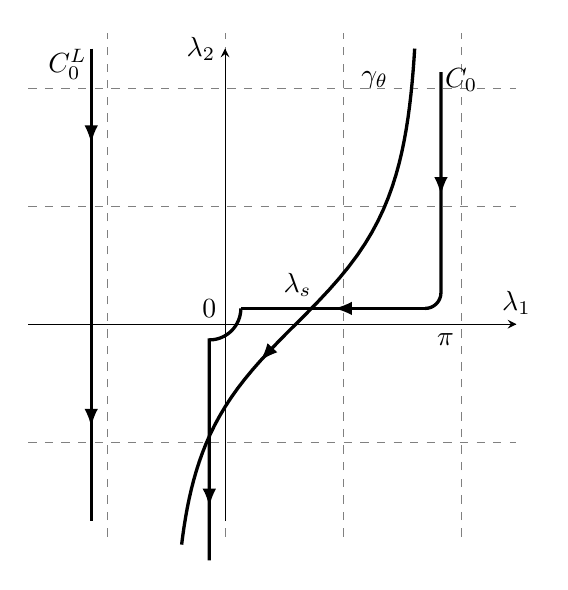
\begin{tikzpicture}
	\draw[step=1.5cm,gray,very thin,dashed](-2.5,-2.7)grid(3.7,3.7);
	\draw[thin, decoration={ markings,  
		mark=at position 1 with {\arrow{stealth}}},
	postaction={decorate}] (-2.5,0)  -- (3.7,0) node[above]{$\lambda_1$};
	\draw[thin, decoration={ markings,  
		mark=at position 1 with {\arrow{stealth}}},
	postaction={decorate}](0,-2.5)--(0,3.5) node[left]{$\lambda_2$};

	\node at (2.8,-0.2) {$\pi$};
	\node at (-0.2,0.2) {$0$};
	\node at (0.92,0.5) {$\lambda_s$};
	\node at (3,3.1) {$C_0$};
	\node at (1.9,3.1) {$\gamma_{\theta}$};
	\node at (-2.0,3.3) {$C_0^L$};
	
	\draw[black,very thick, decoration={ markings,  
		mark=at position 0.2 with {\arrow{latex}},
		mark=at position 0.8 with {\arrow{latex}}},
	postaction={decorate}] (-1.7,3.5)--(-1.7,-2.5);
	
	\draw[black,very thick][domain=0:3.5] plot({2*pi/7 + acos(1/cosh(\x))*pi/180},\x);
	\draw[black,very thick, decoration={ markings,  
		mark=at position 0.2 with {\arrow{latex}}},
	postaction={decorate}][domain=0:-2.8] plot({2*pi/7 - acos(1/cosh(\x))*pi/180},\x);
	
	\draw[very thick,black,%xshift=0pt,
	decoration={ markings,  
		mark=at position 0.8 with {\arrow{latex}}},
	postaction={decorate}]
	(0.2,0.2) arc (0:-90:0.4) -- (-0.2,-3); 
	
	\draw[very thick,black,%yshift=0pt,
	decoration={ markings, mark=at position 0.5 with {\arrow{latex}}}, postaction={decorate}]
	(pi-0.57,0.2) -- (0.2,0.2);

	\draw[very thick,black,%xshift=0pt,
	decoration={ markings,  
		mark=at position 0.5 with {\arrow{latex}}},
	postaction={decorate}]
	(pi-0.4,3.2) -- (pi-0.4,0.4) arc (0:-90:0.2) ;

	\end{tikzpicture}
	\caption{Contours $C_0$ and $\gamma_{\theta}$ in the complex plane $\lambda=\lambda_1+i\lambda_2$. The stationary phase points are noted $\lambda_s$.}
	\label{C4:steepestcontour}
\end{figure}

The far-field evaluation of the integral is obtained by applying the steepest descent method, presented in appendix \ref{PhaseStationnaire}, to \eqref{C4:v1C0}. To do so, contour $C_0$ is deformed into contour $\gamma_{\theta}$, also visible in Fig.~\ref{C4:steepestcontour}. In the case $\nuti_L \in \mathbb{R}$, this leads to
\begin{equation}
v_1=v_1^{sing}+v_1^{diff}
\end{equation}
where $v_1^{sing}$ is the contribution of all the singularities of the spectral functions crossed during the deformation from $C_0$ to $\gamma_{\theta}$, corresponding to the reflected and head waves, and $v_1^{diff}$ is the contribution of the stationary phase point, corresponding to the diffracted wave and computed using \eqref{steepformula}. Only the contribution of the diffracted waves will be computed here. In order to simplify notations, we will note $\mathbf{P}_*(\lambda,1)=\mathbf{P}_*(\lambda)$ and $\mathbf{P}_*(\lambda,-1)=\mathbf{P}_*(-\lambda)$). The contribution of diffracted waves is 
\begin{equation}
v_1^{diff}(R\cos\theta,R\sin\theta)=\frac{e^{-i\pi/4}}{2\sqrt{2\pi}}\sum_{*=L,T}\tilde{\nu}_*^2\frac{e^{-i\tilde{\nu}_*R\cos\delta}}{\sqrt{\nuti_*R\cos\delta}}\mathbf{P_*}(\pi-\theta)\Sigma_1(-\tilde{\nu}_*\cos\theta)
\end{equation}
Analogously,
\begin{equation}
v_2^{diff}(R\cos(\varphi-\theta),R\sin(\varphi-\theta))=\frac{e^{-i\pi/4}}{2\sqrt{2\pi}}\sum_{*=L,T}\tilde{\nu}_*^2\frac{e^{-i\tilde{\nu}_*R\cos\delta}}{\sqrt{\nuti_*R\cos\delta}}\mathbf{P_*}(\pi-(\varphi-\theta))\Sigma_1(-\tilde{\nu}_*\cos(\varphi-\theta))
\end{equation}

In the case where $\nuti_L=i\eta_L \in i\mathbb{R}$, the far-field evaluation is obtained by applying the steepest descent method, presented in appendix \ref{PhaseStationnaire}, to \eqref{C4:v1C0evan}. Contour $C_0$ is deformed into contour $\gamma_{\theta}$ and contour $C_0^L$ is deformed into contour $\gamma_{\theta}^L$. This leads to
\begin{equation}
v_1=v_1^{sing}+v_1^{diff}+v_1^{evan}
\end{equation}
where $v_1^{sing}$ is the contribution of all the singularities of the spectral functions crossed during the deformation from $C_0$ to $\gamma_{\theta}$, $v_1^{diff}$ is the contribution of the stationary phase point to the integral on $C_0$, corresponding to the diffracted wave, and $v_1^{evan}$ is the contribution of the integral on $C_0^L$, which decays exponentially as the far-field parameter $R$ grows, making it an evanescent wave. Once again, only the contribution of the diffracted waves will be computed here. Contribution $v_1^{diff}$ is computed using \eqref{steepformula} :
%. The contribution of evanescent waves is 
%\begin{equation}
%v^{evan}_1(R\cos\theta,R\sin\theta)= \sqrt{\frac{2\pi}{R\eta_L\cos\delta_{\beta}}} e^{-R\eta_L\cos\delta}\mathbf{P_L}(-\theta)\Sigma_1(i\eta_L\cos\theta)
%\end{equation}
%and the contribution of diffracted waves is :
\begin{equation}
v_1^{diff}(R\cos\theta,R\sin\theta)=\frac{e^{-i\pi/4}}{2\sqrt{2\pi}}\tilde{\nu}_T^2\frac{e^{-i\tilde{\nu}_TR\cos\delta}}{\sqrt{\nuti_TR\cos\delta}}\mathbf{P_T}(\pi-\theta)\Sigma_1(-\tilde{\nu}_T\cos\theta)
\end{equation}
Analogously,
%\begin{equation}
%v^{evan}_2(R\cos\theta,R\sin\theta)= \sqrt{\frac{2\pi}{R\eta_L\cos\delta_{\beta}}} e^{-R\eta_L\cos\delta}\mathbf{P_L}(-(\varphi-\theta))\Sigma_1(i\eta_L\cos(\varphi-\theta))
%\end{equation}
%and
\begin{equation}
v_2^{diff}(R\cos\theta,R\sin\theta)=\frac{e^{-i\pi/4}}{2\sqrt{2\pi}}\tilde{\nu}_T^2\frac{e^{-i\tilde{\nu}_TR\cos\delta}}{\sqrt{\nuti_TR\cos\delta}}\mathbf{P_T}(\pi-(\varphi-\theta))\Sigma_2(-\tilde{\nu}_T\cos(\varphi-\theta))
\end{equation}

In both cases, the diffraction coefficient is defined by
\begin{equation}
v_{\beta}^{diff}(R\cos\theta,R\sin\theta)=D_{\beta}^{\alpha}(\theta,\delta)\frac{e^{-i\nuti_{\beta}R\cos\delta_{\beta}}}{\sqrt{\nuti_{\beta}R\cos\delta_{\beta}}} v^{inc}(R\cos\theta,R\sin\theta) \hat{i}_{\beta}
\label{C4:coeffdiff}
\end{equation}
The total diffracted field is
\begin{equation}
v^{diff}=v_1^{diff}+v_2^{diff}
\end{equation}

Let us now isolate L, TH and TV diffracted waves in order to compute the corresponding diffraction coefficients. Using the expressions of the unit vectors given by \eqref{ivec}, the $\beta$ diffracted wave is given by $v^{diff}\cdot \hat{i}_{\beta}$. This yields :
\begin{equation}
D_{\beta}^{\alpha}(\theta,\delta)=\frac{e^{-i\pi/4}}{2\sqrt{2\pi}}\sum_{j=1,2}\nuti_{\beta}^2 \,{}^t \Sigma_j(-\nuti_{\beta}\cos\theta_j)\cdot\left(\mathbf{P}_{\beta}(\pi-\theta_j).\hat{i}_{\beta}\right)
\label{C4:Dbeta}
\end{equation}
where $\theta_1=\theta$ and $\theta_2=\varphi-\theta$.

In order to determine the field diffracted by a wedge illuminated by an incident plane wave, it is sufficient to compute the diffraction coefficient. This coefficient has been expressed in terms of two unknown functions called the spectral functions. The semi-analytical computation of these functions is presented in the following section

\section{Semi-analytical evaluation of the spectral functions}
The first step in computing the spectral functions is to determine a system of functional equations of which they are a solution. We will then show that these functions can be decomposed into two parts : a singular function, computed analytically, and a regular function, approached numerically.
\subsection{Functional equations}
In the previous section, the diffracted wave has been expressed in terms of two unknown functions called the spectral functions. In this subsection, a system of functional equations satisfied by these functions is determined. 

The first step in determining a system of functional equations verified by the spectral functions, is to substitute decomposition \eqref{C4:v1+v2} into the boundary conditions :
\begin{equation}
\left\{
\begin{matrix}
B \big( v_1(x_1,0)+v_2(x_2 \cos \varphi, x_2 \sin \varphi) \big) = -B \rm v_{\alpha}^{inc}|_{\mathcal{S}_1} \\
B \big( v_2(x_2,0)+v_1(x_1 \cos \varphi, x_1 \sin \varphi) \big) = -B \rm v_{\alpha}^{inc}|_{\mathcal{S}_2}
\end{matrix}
\right.
\label{C4:Bivi}
\end{equation}
Let us note $(v_j^1,v_j^2,v_j^3)$ the coordinates of $v_j$ in the Cartesian coordinate system $(x_j,y_j,z_j)$, where $(x_1,y_1,z_1)$ is the coordinate system associated with face $\mathcal{S}_1$ and $(x_2,y_2,z_2)$ is the coordinate system associated with face $\mathcal{S}_2$. These two coordinate systems are linked by (for $j=1,2$):
\begin{equation}
    \left\{
    \begin{matrix}
    x_j=\cos\varphi .x_{3-j}+\sin\varphi. y_{3-j}\\
    y_j=\sin\varphi .x_{3-j}-\cos\varphi .y_{3-j}\\
    z_j=z_{3-j}
    \end{matrix}
    \right.
    \label{C4:changerep}
\end{equation}
Applying \eqref{C4:changerep} to each line of \eqref{C4:Bivi} yields: 
\begin{equation}
\left\{
\begin{matrix}
B_1(v_1)+B_2(v_2)=-Bv_{\alpha}^{inc}|_{\mathcal{S}_1} \\
B_1(v_2)+B_2(v_1)=-Bv_{\alpha}^{inc}|_{\mathcal{S}_2}
\end{matrix}
\right.
\label{C4:b1v1+b2v2}
\end{equation}
where
\begin{equation}
B_1(v)=
\begin{pmatrix}
\mu \left( \frac{\partial v_1}{\partial y_1}+\frac{\partial v_2}{\partial x_1} \right) \\
\frac{\partial v_2}{\partial y_1}+\lambda \left( \frac{\partial v_1}{\partial x_1}+i\tau v_3 \right)\\
\mu \left( \frac{\partial v_2}{\partial z_1}+ \frac{\partial v_3}{\partial y_1}\right)
\end{pmatrix}
\label{C4:B1v1expl}
\end{equation}
and
\begin{equation}
B_2(v)=
\begin{pmatrix}
\mu \sin(2\varphi)\left( \frac{\partial v_1}{\partial x_2}-\frac{\partial v_2}{\partial y_2}\right)-\mu \cos(2\varphi)  \left( \frac{\partial v_1}{\partial y_2}+\frac{\partial v_2}{\partial x_2} \right)\\
(\lambda+2\mu \sin^2\varphi) \frac{\partial v_1}{\partial x_2}+(\lambda+2\mu \cos^2 \varphi)\frac{\partial v_2}{\partial y_2}-\mu \sin(2\varphi)  \left( \frac{\partial v_1}{\partial y_2}+\frac{\partial v_2}{\partial x_2} \right)+\lambda \frac{\partial v_3}{\partial z_2} \\
\mu\sin\varphi\left(\frac{\partial v_3}{\partial x_2}+\frac{\partial v_1}{\partial z_2} \right)-\mu\cos\varphi\left( \frac{\partial v_2}{\partial z_2} +\frac{\partial v_3}{\partial y_2} \right)
\end{pmatrix}
\label{C4:B2v2expl}
\end{equation}
Operator $B_1$ is obtained by projecting $B(v_1)$ onto $\mathcal{S}_1$. This is immediate because $v_1$ is defined on $\mathcal{S}_1$ and its components $(v_1^1,v_1^2,v_1^3)$ are expressed in the associated Cartesian coordinate system $(x_1,y_1,z_1)$. Operator $B_2$ is obtained by projecting $B(v_2)$ onto $\mathcal{S}_1$. This is done by projecting its components $(v_2^1,v_2^2,v_2^3)$ onto $\mathcal{S}_1$ and by expressing $(x_1,y_1,z_1)$ as functions of $(x_2,y_2,z_2)$, as $v_2$ is only defined on $\mathcal{S}_2$. This is done using \eqref{C4:changerep}. The second equation of system \eqref{C4:b1v1+b2v2} is obtained analogously to the first (operators are projected onto $\mathcal{S}_2$ instead of $\mathcal{S}_1$).

The functional equations system solved by the spectral functions is obtained by substituting the integral formulation \eqref{C4:vj0} of $v_1$ and $v_2$ into \eqref{C4:b1v1+b2v2}, evaluating the first equation at $x_1\geq 0, y_1=0$ and the second at $x_2\geq 0, y_2=0$ and applying the Fourier transform to the result. This yields :
\begin{equation}
\begin{split}
\int_0^{+\infty} e^{-ix\xi}B_1(v_1)(x)\,dx&=\frac{1}{2}\textbf{DM}(\Sigma_1)(\xi) \\
&=\frac{1}{2} \int_{\Gamma_0}\textbf{DM}(\xi,\zeta)\Sigma_1(\zeta)\,d\zeta
\end{split}
\label{C4:B1DM}
\end{equation}
where
\begin{equation}
\begin{split}
\textbf{DM}(\xi,\zeta)&=\frac{1}{2i\pi} \frac{1}{\xi-\zeta} \textbf{dm}(\zeta) \\
&=\frac{1}{2i\pi} \frac{1}{\xi-\zeta} \begin{pmatrix}
-1 & \frac{\zeta}{\zeta_T}(1-2\mu Q(\zeta)) & 0\\
-\frac{\zeta}{\zeta_L}(1-2\mu Q(\zeta))  & -1&-\frac{\tau}{\zeta_L}(1-2\mu Q(\zeta)) \\
0&\frac{\tau}{\zeta_T}(1-2\mu Q(\zeta)) &-1
\end{pmatrix}
 \end{split}
\label{C4:defDM}
\end{equation}
and
\begin{equation}
Q(\zeta) =\zeta_L\zeta_T+\zeta^2+\tau^2
\end{equation}
Evaluating $B_2(v_2)$ at $x_1\geq 0, y_1=0$ means is equivalent to evaluating $B_2(v_2)$ at $x_2=x\cos\varphi, y_2=x\sin\varphi, x\geq 0$. The Fourier transform of the second term is therefore
\begin{equation}
\begin{split}
\int_0^{+\infty} e^{-ix\xi}B_2(v_2)(x)\,dx&=\frac{1}{2}\textbf{TM}(\Sigma_2)(\xi) \\
&=\frac{1}{2} \int_{\Gamma_0}\textbf{TM}(\xi,\zeta)\Sigma_2(\zeta)\,d\zeta
\end{split}
\label{C4:B2TM}
\end{equation}
where
\begin{equation}
\textbf{TM}(\xi,\zeta)=\frac{1}{2i\pi}\sum_{*=L,TH,TV}D_*(\xi,\zeta)\textbf{tm}_*(\zeta,\mbox{sgn } \sin \varphi),
\label{C4:defTM}
\end{equation}
$t=$sgn sin $\varphi$,
\begin{equation}
D_*(\xi,\zeta)=\frac{1}{\xi-(\zeta \cos \varphi + \zeta_*(\zeta) |\sin \varphi|)},
\end{equation}
and the following matrices of rank 1 are defined :
\begin{equation}
\left\{
\begin{matrix}
\textbf{tm}_L(\zeta)=\left[ \frac{\zeta}{\zeta_L} f_L\,; \, tf_L\,;  \, \frac{\tau}{\zeta_L}f_L
\right] \\
f_L = \begin{pmatrix}
\mu \lbrack \cos(2\varphi)(2t\zeta\zeta_L)-\sin(2\varphi)(\zeta^2-\zeta_L^2) \rbrack\\
-\lambda+2\mu \lbrack \sin(2\varphi)(t\zeta\zeta_L)-\zeta^2\sin^2\varphi-\zeta^2_L\cos^2\varphi\rbrack\\
-2\mu\tau\lbrack \zeta\sin\varphi -t\zeta_L\cos\varphi\rbrack
\end{pmatrix}
\end{matrix}
\right. ,
\label{C4:tmL}
\end{equation}
\begin{equation}
\left\{
\begin{matrix}
\textbf{tm}_{TH}(\zeta)=\lbrack -tf_{TH}\,;\, \frac{\zeta}{\zeta_T}f_{TH}\,;\, 0 \rbrack\\
f_{TH}=\mu\left(1+\frac{\tau^2}{\zeta^2+\zeta_T^2}\right) \begin{pmatrix}
\sin(2\varphi)(2t\zeta\zeta_T)+\cos(2\varphi)(\zeta^2-\zeta_T^2)\\
\sin(2\varphi)(\zeta^2-\zeta_T^2)-\cos(2\varphi)(2t\zeta\zeta_T)\\
\tau\lbrack t\zeta_T\sin\varphi+\zeta\cos\varphi\rbrack 
\end{pmatrix}
\end{matrix}
\right.
\label{C4:tmTH}
\end{equation}
and
\begin{equation}
\left\{
\begin{matrix}
\textbf{tm}_{TV}(\zeta)=\lbrack \frac{\zeta\tau}{\zeta_T(\zeta^2+\zeta_T^2)}f_{TV}\,;\, \frac{t\tau}{\zeta^2+\zeta_T^2}f_{TV}\,;\, -\frac{1}{\zeta_T}f_{TV} \rbrack\\
f_{TV}=\mu\begin{pmatrix}
\tau\cos(2\varphi)(2t\zeta\zeta_T)-\tau\sin(2\varphi)(\zeta^2-\zeta_T^2)\\
2\tau\lbrack \sin(2\varphi)(t\zeta\zeta_T)-\zeta^2\sin^2\varphi-\zeta_T^2\cos^2\varphi\rbrack\\
\left(\tau^2-\zeta^2+\zeta_T^2\right)\lbrack t\zeta_T\cos\varphi-\zeta\sin\varphi \rbrack
\end{pmatrix}
\end{matrix}
\right.
\label{C4:tmTV}
\end{equation}
In the following, let us note for simplification:
\begin{equation}
\mathbf{tm}_T=\mathbf{tm}_{TH}+\mathbf{tm}_{TV}
\end{equation}

It has been checked that setting $\tau=0$ in the explicit expressions of $\mathbf{DM}$ and $\mathbf{TM}$ operators leads to the same expressions as those found in the previous chapter, concerning the 2D case.

Finally, the Fourier transform of the boundary conditions on the wedge faces its obtained by summing \eqref{C4:B1DM} and \eqref{C4:B2TM}. The right-hand side of the system is obtained by taking the Fourier transform of $-Bv_{\alpha}^{inc}|_{\mathcal{S}_j}, \; j=1,2$. The final system of functional equations solved by the spectral functions is 
\begin{equation}
\left\{
\begin{matrix}
\textbf{DM}(\Sigma_1)+\textbf{TM}(\Sigma_2)=\dfrac{W_1^{\alpha}}{\xi-\nu_{\alpha} \cos \theta_{inc}\cos\delta_{inc}} 
\\
\textbf{TM}(\Sigma_1)+\textbf{DM}(\Sigma_2)=\dfrac{W_2^{\alpha}}{\xi-\nu_{\alpha}\cos(\varphi-\theta_{inc})\cos\delta_{inc}}
\end{matrix}
\right.
\label{C4:equationsintegrales}
\end{equation}
where
\begin{eqnarray}
\begin{array}{lr}
W_1^L=-2\begin{pmatrix}
\mu\cos^2\delta_{inc}\sin(2\theta_{inc}) \\
1-2\mu(\cos^2\theta_{inc}\cos^2\delta_{inc}+\sin^2\delta_{inc})\\
\mu\sin(2\delta_{inc})\sin(\theta_{inc})
\end{pmatrix}\\
~\\
 W_2^L=-2\begin{pmatrix}
\mu\cos^2\delta_{inc}\sin(2\varphi-2\theta_{inc}) \\
1-2\mu(\cos^2(\varphi-\theta_{inc})\cos^2\delta_{inc}+\sin^2\delta_{inc})\\
\mu\sin(2\delta_{inc})\sin(\varphi-\theta_{inc})
\end{pmatrix}\\ 
~\\
W_1^{TV}=2\nu_T\mu\begin{pmatrix}
\frac{1}{2}\sin(2\theta_{inc})\sin(2\delta_{inc})
\\
\sin(2\delta_{inc})\sin^2\theta_{inc}\\
-\sin\theta_{inc}\cos(2\delta_{inc})
\end{pmatrix}~
W_2^{TV}=2\nu_T\mu\begin{pmatrix}
\frac{1}{2}\sin(2\varphi-2\theta_{inc})\sin(2\delta_{inc})
\\
\sin(2\delta_{inc})\sin^2(\varphi-\theta_{inc})\\
-\sin(\varphi-\theta_{inc})\cos(2\delta_{inc})
\end{pmatrix} \\
~
\\
W_1^{TH}=-2 \nu_T\mu \begin{pmatrix}
\cos\delta_{inc}\cos(2\theta_{inc})
\\
\sin(2\theta_{inc})\cos\delta_{inc}\\
\cos\theta_{inc}\sin\delta_{inc}
\end{pmatrix}
~
W_2^{TH}=2 \nu_T\mu \begin{pmatrix}
\cos\delta_{inc}\cos(2\varphi-2\theta_{inc})\\
\sin(2\varphi-2\theta_{inc})\cos\delta_{inc}\\
\cos(\varphi-\theta_{inc})\sin\delta_{inc}
\end{pmatrix}
\end{array}
\label{C4:Wj}
\end{eqnarray}

Thanks to these functional equations, the spectral functions can be decomposed into two parts : a singular function and a regular function. The evaluation of each of these parts is described in the following.

\subsection{Singular part}
\label{C4:singpart}
The first step in evaluating the spectral functions is to determine their poles and corresponding residues. As in the previous chapters, this is done using to a recursive procedure, in which the following translation appears (for $*=L,T$) :
\begin{equation}
\begin{split}
T_*(\xi)&=\xi \cos \varphi+\zeta_*(\xi)\sin \phiti \\
&=\tilde{\nu}_*\cos(\theta+\tilde{\varphi})
\end{split}
\end{equation}
where $\phiti$ is defined in \eqref{phitilde}. This translation operator is defined on subspace $\Omega_*^+$, represented on Fig.~\ref{C4:domega0} :
\begin{equation}
\xi \in \Omega_*^+= \{ \xi=\tilde{\nu}_* \cos \theta, \; 0 \leq \mbox{Re} \theta < \pi-\tilde{\varphi} \}
\label{C4:defOmega0}
\end{equation}
In order to determine the action of operator $\mathbf{DM}$ on a simple pole, contour $\Gamma_0$ in \eqref{C4:B1DM} is deformed into contour $\Gamma_1$, visible in Fig.~\ref{C4:gamma1noncr} for the case $\nuti_L \in \mathbb{R}$ and in Fig.~\ref{C4:gamma1cr} for the case $\nuti_L \in i\mathbb{R}$. In both cases, Cauchy's residue theorem is applied, yielding for $V \in \mathbb{C}^3$, Im$z\geq 0, \, z \notin \{\pm\tilde{\nu}_L,\pm\tilde{\nu}_T \}$, Im$\xi <0 $ with $z\in \mathbb{C} \backslash  \rbrack - \infty, -\nuti_L \rbrack$ if $\noncr$ and $ z\in \mathbb{C} \backslash ( \, \rbrack - \infty, -\nuti_T \rbrack \cup \lbrack \nuti_L,+i\infty \lbrack \,)$ if $\crit$ :
\begin{equation}
\int_{\Gamma_0} \textbf{DM}(\xi,\zeta).\frac{V}{\zeta-z}\,d\zeta = \frac{\textbf{dm}(z).V}{\xi-z}+D_p(z,\xi),
\label{C4:GaussDM}
\end{equation}
where
\begin{equation}
D_p(z,\xi)= \int_{\Gamma_1} \frac{\textbf{DM}(\xi,\zeta)}{\zeta-z}\,d\zeta
\label{C4:defDp}
\end{equation}

\begin{figure}
\centering
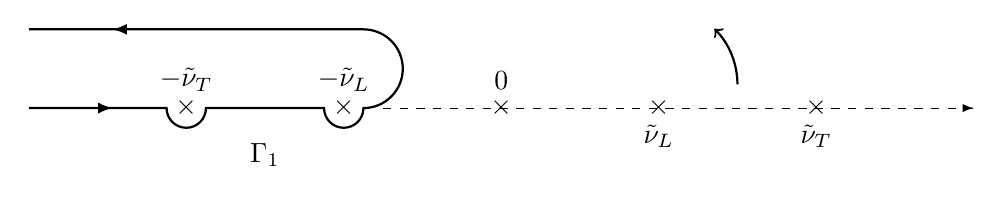
\begin{tikzpicture}
\node at (0,0) {$\times$};
\node at (0,0.35) {$0$};
\node at (2,0) {$\times$}; % Pole
\node at (4,0) {$\times$}; %pole
\node at (2,-0.36) {$\tilde{\nu}_L$};
\node at (4,-0.36) {$\tilde{\nu}_T$};

\node at (-2,0) {$\times$};
\node at (-4,0) {$\times$};
\node at (-2,0.36) {$-\tilde{\nu}_L$}; %pole
\node at (-4,0.36) {$-\tilde{\nu}_T$}; %pole
\node at (-3,-0.6) {$\Gamma_1$};

\draw[dashed, decoration={markings,
 mark=at position 1.0 with {\arrow{latex}}},
      postaction={decorate}] (-1.5,0) -- (6,0);
      
\draw[ thick, ->] (3.0,0.3) arc (0:45:1); %ici c'est les fleches 
  

\draw[thick, black, yshift=0pt,
decoration={ markings,  % This schema allows for fine-tuning the positions of arrows 
      mark=at position 0.1 with {\arrow{latex}},
      mark=at position 0.9 with {\arrow{latex}}},
      postaction={decorate}]
      (-6,0) -- (-4.25,0)  arc (-180:0:0.25) -- (-2.25,0)  arc (-180:0:0.25) -- (-1.75,0) arc(-90:90:0.5)  -- (-6,1);
\end{tikzpicture}
\caption{Contour $\Gamma_1$ in the case $\noncr$. The arrow shows the deformation of contour $\Gamma_0$ into $\Gamma_1$.}
\label{C4:gamma1noncr}
\end{figure}

\begin{figure}
\centering
\begin{subfigure}[b]{0.45\textwidth}
\begin{tikzpicture}[scale=0.8]
\node at (0,0) {$\times$};
\node at (0.35,0.35) {$0$};
\node at (0,1.5) {$\times$}; 
\node at (3,0) {$\times$}; 
\node at (-0.36,1) {$\tilde{\nu}_L$};
\node at (3,-0.36) {$\tilde{\nu}_T$};

\node at (0,-1.5) {$\times$};
\node at (-3,0) {$\times$};
\node at (-0.5,-1.5) {$-\tilde{\nu}_L$}; 
\node at (-3,0.36) {$-\tilde{\nu}_T$};
%\node at (-3,-0.6) {$\Gamma_1^a$};
%\node at (1,3) {$\Gamma_1^b$};

\draw[dashed, decoration={markings,
 mark=at position 1.0 with {\arrow{>}}},
      postaction={decorate}] (-2.5,0) -- (4,0);
      
\draw[dashed, decoration={markings,
 mark=at position 1.0 with {\arrow{>}}},
      postaction={decorate}] (0,-2.5) -- (0,4);

\draw[thick, black, yshift=0pt,
decoration={ markings,  % This schema allows for fine-tuning the positions of arrows 
      mark=at position 0.1 with {\arrow{latex}},
      mark=at position 0.9 with {\arrow{latex}}},
      postaction={decorate}]
      (-5,0) -- (-3.25,0)  arc (-180:0:0.25) -- (-2.75,0) arc(-90:90:0.5)  -- (-3.7,1);
      
\draw[thick, black, yshift=0pt,
decoration={ markings,  
      mark=at position 0.1 with {\arrow{latex}},
      mark=at position 0.9 with {\arrow{latex}}},
      postaction={decorate}]
      (-0.5,3.0) -- (-0.5,1.6) arc(0:180:-0.5)  -- (0.5,4);

\draw[ thick, ->] (-3,3)--(-3.7,3.7);
      
\draw[thick, black, yshift=0pt, decoration={ markings,  
      mark=at position 0.5 with {\arrow{latex}}},
      postaction={decorate}]
      (-3.7,1)arc(180:63.8:2.2);
\end{tikzpicture}
\caption{Intermediate contour $\Gamma_1$. The arrow shows the direction of the deformation.}
\end{subfigure}
~
\begin{subfigure}[b]{0.45\textwidth}
\begin{tikzpicture}[scale=0.8]
\node at (0,0) {$\times$};
\node at (0.35,0.35) {$0$};
\node at (0,1.5) {$\times$}; 
\node at (3,0) {$\times$}; 
\node at (-0.36,1) {$\tilde{\nu}_L$};
\node at (3,-0.36) {$\tilde{\nu}_T$};

\node at (0,-1.5) {$\times$};
\node at (-3,0) {$\times$};
\node at (-0.5,-1.5) {$-\tilde{\nu}_L$}; 
\node at (-3,0.36) {$-\tilde{\nu}_T$};
\node at (-3,-0.6) {$\Gamma_1^a$};
\node at (1,3) {$\Gamma_1^b$};

\draw[dashed, decoration={markings,
 mark=at position 1.0 with {\arrow{>}}},
      postaction={decorate}] (-2.5,0) -- (4,0);
      
\draw[dashed, decoration={markings,
 mark=at position 1.0 with {\arrow{>}}},
      postaction={decorate}] (0,-2.5) -- (0,3.5);

\draw[thick, black, yshift=0pt,
decoration={ markings,  % This schema allows for fine-tuning the positions of arrows 
      mark=at position 0.1 with {\arrow{latex}},
      mark=at position 0.9 with {\arrow{latex}}},
      postaction={decorate}]
      (-5,0) -- (-3.25,0)  arc (-180:0:0.25) -- (-2.75,0) arc(-90:90:0.5)  -- (-5,1);
      
\draw[thick, black, yshift=0pt,
decoration={ markings,  % This schema allows for fine-tuning the positions of arrows 
      mark=at position 0.1 with {\arrow{latex}},
      mark=at position 0.9 with {\arrow{latex}}},
      postaction={decorate}]
      (-0.5,3.5) -- (-0.5,1.6) arc(0:180:-0.5)  -- (0.5,3.5);
      
\end{tikzpicture}
\caption{Final contour $\Gamma_1=\Gamma_1^a \cup \Gamma_1^b$}
\end{subfigure}
\caption{Deformation of contour $\Gamma_0$ onto contour $\Gamma_1=\Gamma_1^a \cup \Gamma_1^b$ in the case $\crit$.}
\label{C4:gamma1cr}
\end{figure}

Similarly, in order to determine the action of operator $\mathbf{TM}$ on a simple pole, contour $\Gamma_0$ in \eqref{C4:B2TM} is deformed into contour $\partial \Omega_L$ for the L terms and $\partial \Omega_T$ for the T terms, both of these are visible in Fig.~\ref{C4:domegaT} for the case $\noncr$. Cauchy's residue theorem is applied, yielding, for $V \in \mathbb{C}^3$, Im$z\geq 0, \, z \notin \{\pm\tilde{\nu}_L,\pm\tilde{\nu}_T \}$, Im$\xi <0 $ with $z\in \mathbb{C} \backslash  \rbrack - \infty, -\nuti_L \rbrack$ :
\begin{equation}
\int_{\Gamma_0} \textbf{TM}(\xi,\zeta).\frac{v}{\zeta-z}\,d\zeta = \sum_{*=L,T} \frac{\textbf{tm}_*(z).v}{\xi-T_*(z)}\textbf{1}_{\Omega_*}(z)+\mathbf{T_p}(z,\xi).v
\label{C4:GaussTM}
\end{equation}
where $\textbf{1}_{\Omega_*}(z)=1$ if $z\in \Omega_*$ and $\textbf{1}_{\Omega_*}(z)=0$ elsewhere and
\begin{equation}
\mathbf{T_p}(z,\xi)= \frac{1}{2i\pi} \sum_{*=L,T} \int_{\partial \Omega_*} D_*(\xi,\zeta) .\dfrac{\textbf{tm}_*(\zeta)}{\zeta-z}\, d\zeta
\end{equation}

\begin{figure}
\centering
\begin{subfigure}[b]{0.45\textwidth}
   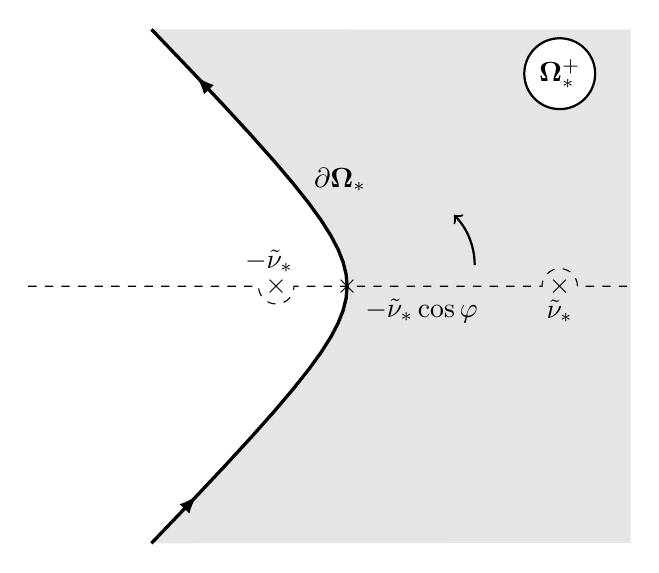
\begin{tikzpicture}[scale=0.9]
% Remplissage espace Omega_0
\fill [color=gray!20]
(3,-3.62) -- plot [domain=-2:2] ({-cosh(\x)},{sinh(\x)}) -- (3,3.62);
%(3,0) -- plot [domain=0:2] ({-cosh(\x)},{sinh(\x)}) -- (3,3.62) -- cycle;
\fill[color=white] (2,3) circle (0.5);
%\fill [color=white] (2,0) circle (0.25);

\node at (2,0) {$\times$};
\node at (2,-0.35) {$\tilde{\nu}_*$};
\node at (-2,0) {$\times$};
\node at (-1,0) {$\times$};
\node at (-2.1,0.35) {$-\tilde{\nu}_*$}; 
\draw[dashed]
      (-5.5,0) -- (-2.25,0)  arc (-180:0:0.25)  -- (1.75,0)arc (180:0:0.25) -- (3,0); 
\draw[black, very thick,decoration={ markings,  
      mark=at position 0.1 with {\arrow{latex}},
      mark=at position 0.9 with {\arrow{latex}}},
      postaction={decorate}][domain=-2:2] plot({-cosh(\x)}, {sinh(\x)});
\node at (-1.1,1.5) {$\mathbf{\partial \Omega_*}$};
\node at (0.05,-0.35) {$-\nuti_*\cos \varphi$};

% Espace Omega_0
\draw[thick] (2,3) circle (0.5);
\node at (2,3) {$\mathbf{\Omega_*^+}$};

\draw[ thick, ->] (0.8,0.3) arc (0:45:1); %ici c'est les fleches 
%\node at (1.2,0.8) {$\mathbf{\mathcal{F}_2}$}; 
\end{tikzpicture}
\caption{Contour $\partial \Omega_*$ and domain $\Omega_*^+$ in the case $\noncr$. The curved arrow shows deformation of contour $\Gamma_0$ onto $\partial \Omega_*$.}
\label{C4:domegaT}     
\end{subfigure}
\hfill
\begin{subfigure}[b]{0.45\textwidth}
   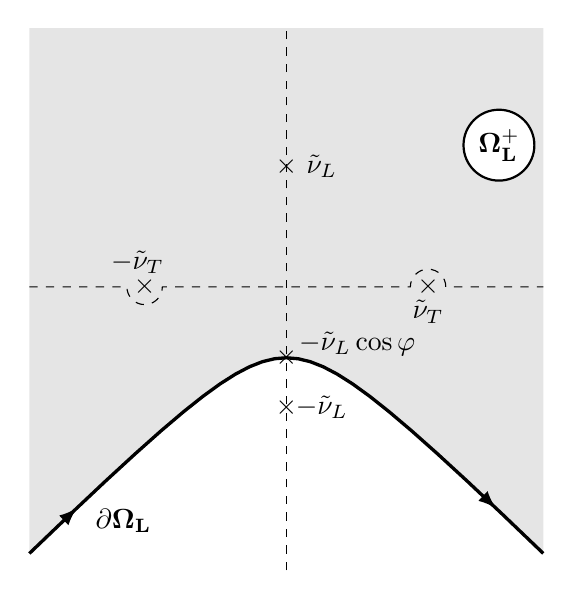
\begin{tikzpicture}[scale=0.9]
\fill [color=gray!20]
(-3.6269,3.65) -- plot [domain=-2:2] ({sinh(\x)},{-cosh(\x)}) -- (3.6269,3.65) ;
\fill[color=white] (3,2) circle (0.5);
\node at (2,0) {$\times$}; 
\node at (0,-1) {$\times$};
\node at (0,1.7) {$\times$};
\node at (0,-1.7) {$\times$};
\node at (2,-0.35) {$\tilde{\nu}_T$};
\node at (-2,0) {$\times$};
\node at (-2.1,0.35) {$-\tilde{\nu}_T$}; 
\draw[dashed]
      (-3.6269,0) -- (-2.25,0)  arc (-180:0:0.25)  -- (1.75,0)arc (180:0:0.25) -- (3.6269,0); % ca c'est l'axe
\draw[dashed] (0,-4) -- (0,3.65);
% Hyperbole (contour  partial_Omega_0 )
\draw[black, very thick,decoration={ markings,  % This schema allows for fine-tuning the positions of arrows 
      mark=at position 0.1 with {\arrow{latex}},
      mark=at position 0.9 with {\arrow{latex}}},
      postaction={decorate}][domain=-2:2] plot({sinh(\x)},{-cosh(\x)});
\node at (1,-0.8) {$-\nuti_L\cos\varphi$};
\node at (0.5,1.7) {$\nuti_L$};
\node at (0.5,-1.7) {$-\nuti_L$};
\node at (-2.3,-3.3) {$\mathbf{\partial \Omega_L}$};

% Espace Omega_0
\draw[thick] (3,2) circle (0.5);
\node at (3,2) {$\mathbf{\Omega_L^+}$};
\end{tikzpicture}
\caption{Contour $\partial \Omega_L$ and domain $\Omega_L^+$ in the case $\crit$.}
\label{C4:domegaL}
\end{subfigure}
\caption{Domains $\Omega_*$ and contours $\partial \Omega_*$ in cases $\noncr$ and $\crit$.}
\label{C4:domega0}
\end{figure}

In the case where $\crit$, $\partial \Omega_L$ is visble in Fig.~\ref{C4:domegaL}. During the deformation of contour $\Gamma_0$ into contour $\partial\Omega_L$, the pole $z$ is not crossed  and therefore does not contribute to the integral. However, if there exists $\zeta_0 \in \Omega_L^+$ such that $T_L(\zeta_0)=\xi$ and Im$\zeta_0<0$, then pole $\zeta_0$ is crossed during this deformation. Let us now determine when this is possible. Suppose that $\zeta_0=\nuti_L\cos\theta_0=\nuti_L\cos(\theta_0'+i\theta_0'')$ and $\xi=T_L(\zeta_0)=\nuti_L\cos(\theta_0+\phiti)$ and $\nuti_L=i\eta_L \in i\mathbb{R}$, we then have :
\begin{equation}
\rm Im \zeta_0=\eta_L\cos\theta_0'\cosh\theta_0''  
\end{equation}
Combining the facts that Im$\zeta_0<0$ and $\zeta_0 \in \Omega_L^+$ gives
\begin{equation}
\dfrac{\pi}{2}<\theta_0'<\pi-\phiti
\label{C4:condcr}
\end{equation}
Condition \eqref{C4:condcr} has solutions if and only if $\phit<\dfrac{\pi}{2}$. From hereon after, we will suppose that this is not the case. In practice, this is not too restrictive since, as explained in \ref{Chapter5:sing_part}, the spectral functions method is less accurate for small wedge angles.

It is important to note that in all the aforementioned contour deformations, no branch points of the integrands are crossed. Therefore, it is assumed that Croisille and Lebeau's \cite{CroisilleLebeau} proof that $\mathbf{D_p}(z,\cdot)$ and $\mathbf{T_p}(z,\cdot)$ belong to a special class of functions $\mathcal{H}^3$ can be adapted to the 3D case. It will therefore be assumed that in the case $\noncr$, $\mathbf{D_p}(z,\cdot) \in \mathcal{H}^3$ and $\mathbf{T_p}(z,\cdot) \in \mathcal{H}^3$ and in the case $\crit$, $\mathbf{D_p}(z,\cdot) \in \tilde{\mathcal{H}}^3$ and $\mathbf{T_p}(z,\cdot) \in \mathcal{H}^3$. $\mathcal{H}$ and $\tilde{\mathcal{H}}$ are defined hereafter
\begin{definition}
\label{C4:defH}
$\mathcal{H}$ is the space of the functions f analytical in $\mathbb{C}\backslash \rbrack -\infty,-\nuti_L\rbrack$ such that $\forall \epsilon \in \rbrack0,\pi \lbrack, f(e^{i\epsilon} \cdot)\in H^+$, where $H^+$ is defined in Def.~\ref{defHpl}.
\end{definition}
\begin{definition}
\label{C4:defHcrit}
$\tilde{\mathcal{H}}$ is the space of the functions f analytical in  $\mathbb{C} \backslash ( \, \rbrack - \infty, -\nuti_T \rbrack \cup \lbrack \nuti_L,+i\infty \lbrack \,)$ such that $\forall \epsilon \in \rbrack0,\pi \lbrack, f(e^{i\epsilon} \cdot)\in H^+$, where $H^+$ is defined in Def.~\ref{defHpl}.
\end{definition}

Let us now extract all the poles and corresponding residues of the spectral functions, using system \eqref{C4:equationsintegrales} and results \eqref{C4:GaussDM} and \eqref{C4:GaussTM}. We begin with the following decomposition, for Im $\xi \le 0$ : 
\begin{equation}
\Sigma_j(\xi)= \frac{V_j^{(0)}}{\xi-Z^{(0)}_j}+X'_j(\xi)
\label{C4:extraction1}
\end{equation}
where $V_j^{(0)}$ are to be determined, $X'_j$ is an unknown function and
\begin{subequations}
\begin{equation}
Z_1^{(0)}=\nu_{\alpha} \cos \theta_{inc}\cos\delta_{inc}=\nuti_{\alpha}\cos\theta_{inc},
\end{equation}
\begin{equation}
Z_2^{(0)}=\nu_{\alpha} \cos(\varphi-\theta_{inc})\cos\delta_{inc}=\nuti_{\alpha}\cos(\varphi-\theta_{inc}).
\end{equation}
\end{subequations}
Substituting \eqref{C4:extraction1} into \eqref{C4:equationsintegrales} and applying \eqref{C4:GaussDM} yields
\begin{eqnarray}
\left\{
\begin{array}{l}
\textbf{DM}(X'_1)+\textbf{TM}(X'_2)+\textbf{TM}(\frac{V_2^{(0)}}{\xi-Z_2^{(0)}})=\frac{W^1_{\alpha}}{\xi-Z_1^{(0)}}-\frac{\textbf{dm}(Z_1^{(0)}).V_1^{(0)}}{\xi-Z_1^{(0)}}-\mathbf{D_p}(Z_1^{(0)},\xi).V_1^{(0)} \\
~
\\
\textbf{TM}(X'_1)+\textbf{DM}(X'_2)+\textbf{TM}(\frac{V_1^{(0)}}{\xi-Z_1^{(0)}})=\frac{W^2_{\alpha}}{\xi-Z_2^{(0)}}-\frac{\textbf{dm}(Z_2^{(0)}).V_2^{(0)}}{\xi-Z_2^{(0)}}-\mathbf{D_p}(Z_2^{(0)},\xi).V_2^{(0)} 
\end{array}
\right.
\label{C4:mille}
\end{eqnarray}
The singular terms in the right-hand side of this system are eliminated by setting
\begin{equation}
V_j^{(0)}=\textbf{dm}^{-1}(Z_j^{(0)}).W_j^{\alpha}
\end{equation}
In all the following, we will suppose that we have det$(\mathbf{dm}) \neq 0$. Applying \eqref{C4:GaussTM} reveals two new poles, leading to a second decomposition 
\begin{equation}
X'_j=X''_j+\frac{V_{j,L}^{(1)}}{\xi-Z_{j,L}^{(1)}}+\frac{V_{j,T}^{(1)}}{\xi-Z_{j,T}^{(1)}}
\end{equation}
where, for $*=L,T$ 
\begin{equation}
Z_{j,*}^{(1)}=T_*(Z_{3-j}^{(0)})
\end{equation}
and $V_{j,*}^{(1)}$ remain to be determined. Once again, they are chosen so as to eliminate the singular terms in the right-hand side of the system :
\begin{equation}
V_{j,*}^{(1)}=-\mathbf{dm}^{-1}(T_*(Z_{j}^{(0)})).\mathbf{tm_*}(Z_{3-j}^{(0)}).V_{3-j}^{(0)}
\end{equation}
These steps are repeated recursively as long as $\textbf{1}_{\Omega_L}(Z_{j,*}^{(k)}=1$ and $\textbf{1}_{\Omega_T}(Z_{j,*}^{(k)}=1$. In the end, we have, for  $\mbox{Im} \xi <0$
\begin{gather}
\Sigma_j(\xi)=Y_j(\xi)+X_j(\xi) \label{C4:decomp}\\
Y_j(\xi)=\sum_k \sum_{*=L,T} \frac{V_{j,*}^{(k)}}{\xi-Z_{j,*}^{(k)}}
\label{C4:yj},
\end{gather}
where
\begin{equation}
\begin{matrix}
Z_{1}^{(0)}=\nu_{\alpha} \cos \theta_{inc},  & Z_{2}^{(0)}=\nu_{\alpha} \cos(\varphi-\theta_{inc}) \\
Z_{j,L}^{(k+1)}= T_L(Z_{3-j,*}^{(k)}) &Z_{j,T}^{(k+1)}= T_T(Z_{3-j,*}^{(k)}) 
\end{matrix}
\label{C4:poles}
\end{equation}
and
\begin{equation}
\begin{matrix}
V_{j}^{(0)}=\textbf{dm}^{-1}(Z_{j}^{(0)}).W_j^{\alpha}\\
V_{j,L}^{(k+1)}=-\textbf{dm}^{-1}(Z_{j,*}^{(k+1)}).\textbf{tm}_L(Z_{3-j,*}^{(k)}).V_{3-j,*}^{(k)}.\textbf{1}_{\Omega_L}(Z_{3-j,*}^{(k)}) \\ 
V_{j,T}^{(k+1)}=-\textbf{dm}^{-1}(Z_{j,*}^{(k+1)}).\textbf{tm}_T(Z_{3-j,*}^{(k)}).V_{3-j,*}^{(k)}.\textbf{1}_{\Omega_T}(Z_{3-j,*}^{(k)}) 
\end{matrix}
\label{C4:residus}
\end{equation}
The recursive procedure stops when $\textbf{1}_{\Omega_L}(Z_{j,*}^{(k)}+\textbf{1}_{\Omega_T}(Z_{j,*}^{(k)}=0$ (meaning when no more poles can be found by deforming contour $\Gamma_0$ into $\partial \Omega_L$ or $\partial \Omega_T$. When $\noncr$, Croisille and Lebeau \cite{CroisilleLebeau} have shown that this defines a finite number of poles. We will now prove that this is still true when $\crit$. Physically, this means that an incident ray exits the wedge after a finite number of reflections and mode conversions.
\begin{lemma}
The number of poles defined recursively by \eqref{C4:poles}, is finite.
\label{C4:finipoles}
\end{lemma}
\paragraph*{Proof.} To prove lemma \ref{C4:finipoles}, it is sufficient to prove that and infinite sequence $(z_l)_{l\geq0}$ of the form
\begin{equation}
z_0 \in \mathbb{C}, \hspace{1em} z_{l+1}=T_{\nuti_l}(z_l), \hspace{1em} z_l\in\Omega_{\nuti_l}, \hspace{1em} \nuti_l=\nuti_L=i\eta_L \rm or \nuti_l=\nuti_T
\end{equation}
does not exist. Suppose we have :
\begin{equation}
\begin{split}
z_l&=\nuti_l\cos\theta_l=\nuti_l\cos(\theta_1^l+i\theta_2^l)\\
&=\nuti_l(\cos\theta_1^l\cosh\theta_2^l-i\sin\theta_1^l\sinh\theta_2^l
\end{split}
\end{equation}
with $0\leq \theta_1^l\leq \pi-\phiti$. Then, if $\nuti_l=\nuti_T$ :
\begin{equation}
\begin{split}
\rm Re(T_T(z_l))&=\nuti_T\cos(\theta_1^l+\phiti)\cosh\theta_2^l\\
&\leq\nuti_T(\cos\theta_1^l-\varepsilon_0)\cosh\theta_2^l\leq \rm Re(z_l)-\nuti_T \varepsilon_0
\end{split}
\end{equation}
where $\varepsilon_0>0$ depends only of $\phiti$. If $\nuti_l=\nuti_L=i\eta_L$, then
\begin{equation}
\begin{split}
\rm Im(T_L(z_l))&=\eta_L\cos(\theta_1^l+\phiti)\cosh\theta_2^l\\
&\leq\eta_L(\cos\theta_1^l-\varepsilon_0)\cosh\theta_2^l\leq \rm Re(z_l)-\eta_L \varepsilon_0
\end{split}
\end{equation}
In both cases, if the number of points $z_l$ is infinite, then $|z_l| \rightarrow +\infty$, implying $|\theta_2^l| \rightarrow +\infty$ and
\begin{equation}
\cosh\theta_2^l \sim |\sinh\theta_2^l| \sim \frac{1}{2} e^{|\theta_2^l|}
\end{equation}
which in turn, implies
\begin{equation}
|\rm arg \, z_l| \sim \theta_1^l \hspace{1em}\rm and \hspace{1em}|\rm arg \,z_{l+1}| \sim \theta_1^l+\phiti \sim \theta_1^{l+1} \Rightarrow \theta_1^l \rightarrow +\infty
\end{equation}
This is impossible. Therefore, the sequence $(z_l)_{l\geq 0}$ is necessarily finite.
\paragraph*{}
We have thus extracted all the poles from the spectral functions and have computed them analytically, along with their corresponding residues.

\subsection{Regular Part}
\label{C4:regpart}
The singular parts $Y_j$ of the spectral functions having been determined, two new functions $X_1$ and $X_2$ are defined by \eqref{C4:decomp}. In the following, a numerical approximation method for $X_j$ is proposed. In order to do so, a system of functional equations solved by $X_1, X_2$ is derived by subtracting vector
\begin{equation}
\begin{pmatrix}
\textbf{DM}(Y_1)+\textbf{TM}(Y_2) \\
\textbf{TM}(Y_1)+\textbf{DM}(Y_2)
\end{pmatrix},
\end{equation}
where $Y_1$ and $Y_2$ are given by equations \eqref{C4:yj} to \eqref{C4:residus}, from both sides of \eqref{C4:equationsintegrales} :
\begin{equation}
\left\{ 
\begin{matrix}
\mathbf{DM}(X_1)(\xi)+\textbf{TM}(X_2)(\xi)=u_1(\xi)\\
\textbf{TM}(X_1)(\xi)+\textbf{DM}(X_2)(\xi)=u_2(\xi)
\end{matrix}
\right.,
\label{C4:regparteqn}
\end{equation}
with, for $j=1,2$
\begin{equation}
u_j(\xi)=-\sum_k \sum_{*=L,T} \left[ \mathbf{D_p}(Z_{j,*}^{(k)},\xi).V_{j,*}^{(k)}+\mathbf{T_p}(Z_{3-j,*}^{(k)},\xi).V_{3-j,*}^{(k)}\right]
\label{C4:scndmembre}
\end{equation}
It is assumed that Croisille and Lebeau's \cite{CroisilleLebeau} proof that this system has a unique solution $(X_1,X_2)$ in $\mathcal{H}^3$ (defined in Def.~\ref{C4:defH}) can be adapted to the 3D case to prove that system \eqref{C4:regparteqn} has a unique solution in $\mathcal{H}^3$ (defined in Def.~\ref{C4:defH} is $\noncr$ and Def.~\ref{C4:defHcrit} if $\crit$). Once again, a numerical approximation of the regular parts $X_j$ will be computed using the Galerkin collocation method. The functional space $\mathcal{H}$ is approached by the finite-dimension subspace generated by basis functions $(\varphi_k)_{1 \leq k \leq 2N}$ defined by \eqref{Gal_basis}, with $(a_k)_{1 \leq k \leq 2N} \in \lbrack \nuti_L, + \infty \lbrack^N$ if $\noncr$ and $(a_k)_{1 \leq k \leq N} \in \lbrack \nuti_T, + \infty \lbrack^N ,\; \; (a_k)_{N+1\leq k \leq 2N} \in \rbrack -i\infty, -\nuti_L\rbrack^N$ if $\crit$. Functions $X_j$ are approximated in this space by :
\begin{equation}
 X_j(\xi) \approx \sum_{k=1}^N \tilde{X}_j^k \varphi_k(\xi) ,\hspace{1em} \tilde{X}_j^k \in \mathbb{C}^3
 \label{C4:Xj}
\end{equation}
Approximation \eqref{C4:Xj} is substituted into \eqref{C4:regparteqn} and the variable change $\zeta=iy$ is applied in the resulting system. This system is then evaluated at $\xi=b_1,...,b_{2N}$, leading to a linear system of equations which can be written in matrix form :
\begin{eqnarray}
\begin{pmatrix}
\mathbb{D}&\mathbb{T}\\
\mathbb{T}&\mathbb{D}
\end{pmatrix}
\begin{pmatrix}
\mathbb{X}_1 \\
\mathbb{X}_2
\end{pmatrix}
=
\begin{pmatrix}
\mathbb{U}_1 \\
\mathbb{U}_2
\end{pmatrix}
\Leftrightarrow
\left\{
\begin{array}{l}
(\mathbb{D}+\mathbb{T})(\mathbb{X}_1+\mathbb{X}_2)= \mathbb{U}_1+\mathbb{U}_2 \\
(\mathbb{D}-\mathbb{T})(\mathbb{X}_1-\mathbb{X}_2)= \mathbb{U}_1-\mathbb{U}_2
\end{array}
	\right.,
\label{C4:systmat}
\end{eqnarray}
where matrices $(6N\times 6N)$ are defined by $3\times3$ blocks:
\begin{equation}
\begin{split}
\mathbb{D}_{lk}&=\int_{-\infty}^{+\infty} \textbf{DM}(b_l,iy)e_{a_k}(y) \, dy =\frac{1}{2i\pi} \int_{-\infty}^{+\infty} \frac{\mathbf{dm}}{b_l-iy} 
%\begin{pmatrix}
%-1&A(iy) \\
%B(iy)&-1
%\end{pmatrix}
\sqrt{\frac{a_k}{\pi}}\frac{1}{y-ia_k} \, dy \\
&=- \frac{\sqrt{a_k}}{2\pi \sqrt{\pi}}
\begin{pmatrix}
\mathcal{D}_1(a,b) &\mathcal{D}_2^T(a,b) &0\\
-\mathcal{D}_2^L(a,b) &\mathcal{D}_1(a,b)&-\mathcal{D}_3^L(a,b)\\
0&\mathcal{D}_3^T(a,b)&\mathcal{D}_1(a,b)
\end{pmatrix}=\frac{\sqrt{a_k}}{2\pi \sqrt{\pi}}\mathbb{D}(a_k,b_l)
\end{split}
\label{C4:Dab}
\end{equation}
where functions $e_{a_k}$ are defined by \eqref{Galerkin_basis} and the explicit expressions of coefficients of matrix $\mathbb{D}(a,b)$ and their values are computed in appendix \ref{finalD3D}. The other matrices involved are, for $1\leq l,k \leq 2N$
\begin{equation}
\begin{split}
\mathbb{T}_{lk}&=\int_{-\infty}^{+\infty} \textbf{TM}(b_l,iy)e_{a_k}(y) \, dy 
=\frac{1}{2i\pi} \int_{-\infty}^{+\infty} \sum_{*=L,T} \frac{\textbf{tm}_* (iy, \mbox{sgn} \sin \varphi)}{b_l-T_*(iy)} \sqrt{\frac{a_k}{\pi}}\frac{1}{y-ia_k}\,dy \\
&=\frac{1}{2i\pi}\sqrt{\frac{a_k}{\pi}}\sum_{*=L,T} \int_{-\infty}^{+\infty} \frac{\textbf{tm}_*(iy,\epsilon)}{\lbrack b_l-(iy \cos \varphi +  \zeta_*(iy)| \sin \varphi|)\rbrack(y-ia_k)} \, dy,
\end{split}
\end{equation}
where $\epsilon= \mbox{sgn}( \sin \varphi)$. Let us define
\begin{equation}
\mathbb{T}_{lk}=\frac{1}{2i\pi}\sqrt{\frac{a_k}{\pi}}
\sum_{*=L,TH,TV}
\begin{pmatrix}
\mathcal{T}_1^*(a,b) &  \mathcal{T}_2^*(a,b) &\mathcal{T}_3^*(a,b) \\
\mathcal{T}_4^*(a,b) &\mathcal{T}_5^*(a,b)&\mathcal{T}_6^*(a,b)\\
\mathcal{T}_7^*(a,b)&\mathcal{T}_8^*(a,b)&\mathcal{T}_9^*(a,b)
\end{pmatrix}
=\frac{1}{2i\pi}\sqrt{\frac{a_k}{\pi}}\mathbb{T}(a_k,b_l)
\label{Tab}
\end{equation}
The explicit expressions of operators $\mathcal{T}_i^*, 1\leq i\leq9, *=L,TH,TV$ and their values are computed in \ref{finalT3D}. Finally:
\begin{equation}
\mathbb{X}_j=
\begin{pmatrix}
\tilde{X}_j^1\\
\vdots \\
\tilde{X}_j^{2N}
\end{pmatrix}
\hspace{3em}
\mathbb{U}_j=
\begin{pmatrix}
u_j(b_1)\\
\vdots \\
u_j(b_{2N})
\end{pmatrix}
\end{equation}
where $u_j(\xi)$ is given by \eqref{C4:scndmembre}. The same considerations as those made in \ref{C3:regpart} lead to an expression of $u_j$ with respect to operators $\mathbb{D}(\cdot,\cdot)$ and $\mathbb{T}(\cdot,\cdot)$ :
\begin{equation}
u_j(\xi)=-\frac{1}{2i\pi}\sum_{k}\sum_{*=L,T}\left(i\mathbb{D}(-Z_{j,*}^{(k)},\xi).V_{j,*}^{(k)}+\mathbb{T}(-Z_{3-j,*}^{(k)},\xi).V_{3-j,*}^{(k)} \right) +\frac{W_j^{\alpha}}{\xi-Z_j^{(0)}}
\label{C4:uDT}
\end{equation}

 Using these results, the linear system \eqref{C4:systmat} is implemented and solved numerically using the C++ library Eigen, and an evaluation of the regular part of the spectral functions is obtained. However, for values of $\xi$ lying in certain parts of the complex plane, this evaluation is not sufficiently accurate. The technique used to solve this problem is called the propagation of the solution.
 
\subsection{Propagation of the solution}
\label{C4:propag}
The method called propagation of the solution is used to propagate the accuracy of the numerical approximation of the regular functions $X_1$ and $X_2$ from parts of the complex plane where they are evaluated accurately to parts of the complex plane where they are not.

\begin{figure}[h]
	\centering
	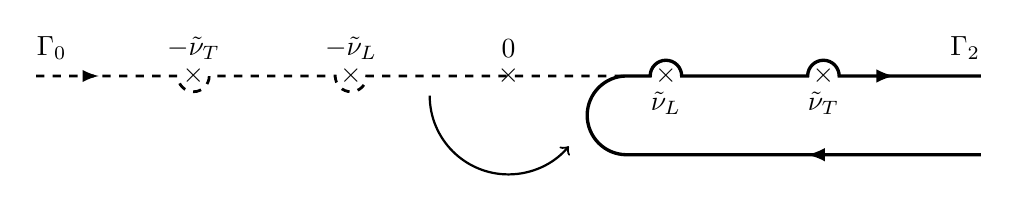
\begin{tikzpicture}
	\node at (0,0) {$\times$};
	\node at (0,0.35) {$0$};
	\node at (2,0) {$\times$}; % Pole
	\node at (2,-0.35) {$\nuti_L$};
	\node at (4,0) {$\times$};
	\node at (4,-0.35) {$\nuti_T$};
	\node at (-2,0) {$\times$};
	\node at (-2,0.35) {$-\nuti_L$};
	\node at (-4,0) {$\times$};
	\node at (-4,0.35) {$-\nuti_T$};
	\node at (5.8,0.35) {$\Gamma_2$};
	\node at (-5.8,0.35) {$\Gamma_0$};
	\draw[very thick, black,yshift=0pt,
	decoration={ markings,
		mark=at position 0.2 with {\arrow{latex}},
		mark=at position 0.9 with {\arrow{latex}}},
	postaction={decorate}]
	(6,-1) -- (1.5,-1)  arc (90:-90:-0.5) -- (1.8,0) arc (180:0:0.2) -- (3.8,0) arc (180:0:0.2) -- (6,0);
	
	\draw[dashed, line width = 1pt,yshift=0pt,
	decoration={ markings,
		mark=at position 0.1 with {\arrow{latex}}},
	postaction={decorate}]
	(-6,0) -- (-4.2,0) arc (-180:0:0.2) -- (-2.2,0)  arc (-180:0:0.2)  -- (1.5,0);
	
	\draw[ thick, ->] (-1,-0.25) arc (180:320:1);
	\end{tikzpicture}
	\caption{Integration contour $\Gamma_2$ in the case $\noncr$. The curved arrow indicates the contour deformation from $\Gamma_0$ to $\Gamma_2$.}
	\label{C4:contour2}
\end{figure}

The first step of this procedure is to deform contour $\Gamma_0$ in operator $\mathbf{DM}$ into contour $\Gamma_2$ in \eqref{C4:regparteqn}. Contour $\Gamma_2$ is visible on Fig.~\ref{C4:contour2} for the case $\noncr$ and in Fig.~\ref{C4:contour2crit} for the case $\crit$. During this deformation, the half-plane Im$\xi<0$ is crossed (with the exception of branch $\lbrack -\nuti_L,-\infty \lbrack$ in the case $\crit$). The contribution of poles $\zeta=\xi$ crossed during this contour deformation is given by Cauchy's residue formula :
\begin{equation}
\int_{\Gamma_0} \textbf{DM}(\xi,\zeta)X_j(\zeta)\, d\zeta = \int_{\Gamma_2}  \textbf{DM}(\xi,\zeta)X_j(\zeta)\, d\zeta + \textbf{dm}(\xi).X_j(\xi)
\label{C4:DM2}
\end{equation}

\begin{figure}
\centering
\begin{subfigure}[b]{0.45\textwidth}
	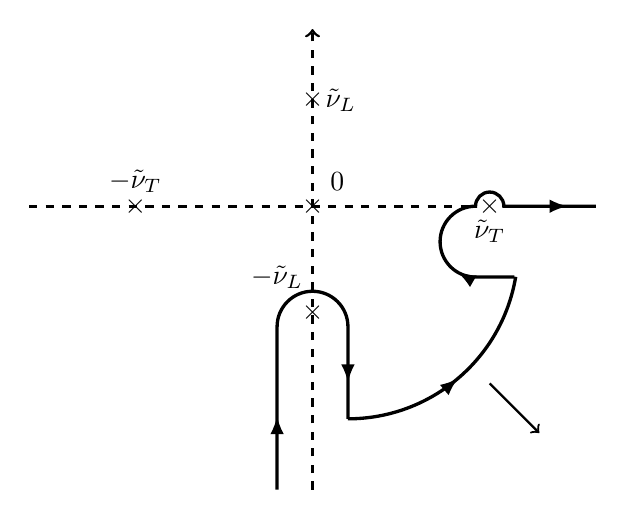
\begin{tikzpicture}[scale=0.9]
	\node at (0,0) {$\times$};
	\node at (0.35,0.35) {$0$};
	\node at (0,1.5) {$\times$}; % Pole
	\node at (0.4,1.5) {$\nuti_L$};
	\node at (2.5,0) {$\times$};
	\node at (2.5,-0.35) {$\nuti_T$};
	\node at (0,-1.5) {$\times$};
	\node at (-0.5,-1) {$-\nuti_L$};
	\node at (-2.5,0) {$\times$};
	\node at (-2.5,0.35) {$-\nuti_T$};
%	\node at (5.8,0.35) {$\Gamma_2^a$};
%	\node at (1,-4) {$\Gamma_2^b$};
%	\node at (-5.8,0.35) {$(\Gamma_0)$};
	
	\draw[very thick, black,yshift=0pt,
	decoration={ markings,  % This schema allows for fine-tuning the positions of arrows 
		mark=at position 0.2 with {\arrow{latex}},
		mark=at position 0.9 with {\arrow{latex}}},
	postaction={decorate}]
	(2.85,-1) -- (2.3,-1)  arc (90:-90:-0.5)  -- (2.3,0) arc (180:0:0.2) -- (4,0);
	
	\draw[very thick, black,yshift=0pt,
	decoration={ markings,  % This schema allows for fine-tuning the positions of arrows 
		mark=at position 0.2 with {\arrow{latex}},
		mark=at position 0.9 with {\arrow{latex}}},
	postaction={decorate}]
	(-0.5,-4) -- (-0.5,-1.7) arc (0:-180:-0.5) -- (0.5,-3);
	
	\draw[very thick, black,yshift=0pt,
	decoration={ markings,mark=at position 0.5 with {\arrow{latex}}},
	postaction={decorate}]
	(0.5,-3) arc (-90:-9.5:2.4);
	
	\draw[dashed, line width =1pt, yshift=0pt,
	decoration={ markings,mark=at position 1 with {\arrow{>}}},
	postaction={decorate}]
	(0,-4)--(0,2.5);
	
%	\draw[dashed, line width = 1pt,yshift=0pt,
%	decoration={ markings,mark=at position 0.1 with {\arrow{latex}}},
%	postaction={decorate}]
%	(-6,0) -- (-3.2,0) arc (-180:0:0.2) -- (2.8,0)arc (180:0:0.2);

\draw[dashed, line width = 1pt,yshift=0pt]
	(-4,0) -- (2.3,0);
	
	\draw[ thick, ->] (2.5,-2.5)--(3.2,-3.2);
	
	\end{tikzpicture}
	\caption{Intermediate contour $\Gamma_2$. The arrow shows the direction of the deformation.}
\end{subfigure}
~
\begin{subfigure}[b]{0.45\textwidth}
	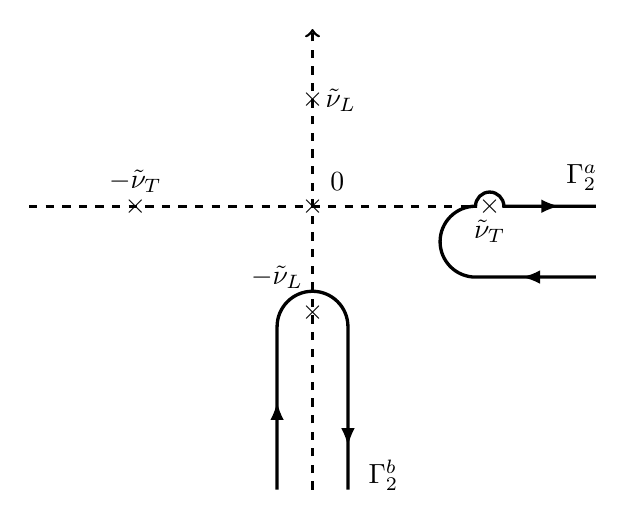
\begin{tikzpicture}[scale=0.9]
	\node at (0,0) {$\times$};
	\node at (0.35,0.35) {$0$};
	\node at (0,1.5) {$\times$}; % Pole
	\node at (0.4,1.5) {$\nuti_L$};
	\node at (2.5,0) {$\times$};
	\node at (2.5,-0.35) {$\nuti_T$};
	\node at (0,-1.5) {$\times$};
	\node at (-0.5,-1) {$-\nuti_L$};
	\node at (-2.5,0) {$\times$};
	\node at (-2.5,0.35) {$-\nuti_T$};
	\node at (3.8,0.4) {$\Gamma_2^a$};
	\node at (1,-3.8) {$\Gamma_2^b$};
%	\node at (-4.8,0.35) {$(\Gamma_0)$};
	
	\draw[very thick, black,yshift=0pt,
	decoration={ markings,  
		mark=at position 0.2 with {\arrow{latex}},
		mark=at position 0.9 with {\arrow{latex}}},
	postaction={decorate}]
	(4,-1) -- (2.3,-1)  arc (90:-90:-0.5)  -- (2.3,0) arc (180:0:0.2) -- (4,0);
	
	\draw[very thick, black,yshift=0pt,
	decoration={ markings, 
		mark=at position 0.2 with {\arrow{latex}},
		mark=at position 0.9 with {\arrow{latex}}},
	postaction={decorate}]
	(-0.5,-4) -- (-0.5,-1.7) arc (0:-180:-0.5) -- (0.5,-4);
	
	\draw[dashed, line width =1pt, yshift=0pt,
	decoration={ markings,mark=at position 1 with {\arrow{>}}},
	postaction={decorate}]
	(0,-4)--(0,2.5);
	
%	\draw[dashed, line width = 1pt,yshift=0pt,
%	decoration={ markings,mark=at position 0.1 with {\arrow{latex}}},
%	postaction={decorate}]
%	(-6,0) -- (-3.2,0) arc (-180:0:0.2) -- (2.8,0)arc (180:0:0.2);

	\draw[dashed, line width = 1pt,yshift=0pt]
	(-4,0) -- (2.3,0);
	
	\end{tikzpicture}
	\caption{Final contour $\Gamma_2=\Gamma_2^a\cup\Gamma_2^b$}
\end{subfigure}
\caption{Deformation of contour $\Gamma_0$ onto contour $\Gamma_2=\Gamma_2^a\cup\Gamma_2^b$ in the case $\crit$.}
\label{C4:contour2crit}
\end{figure}

The next step is to define the inverse translation operator $T_*^{-1}, *=L,T$ :
\begin{equation}
T_*^{-1}(\xi=\nu_*\cos\theta)=\xi \cos \phiti-\zeta_*(\xi)\sin\phiti=\nu_*\cos(\theta-\tilde{\varphi}).
\end{equation}
This operator is well defined on subspace $\Omega_*^-$, visible on Fig.~\ref{C4:dOmegamoins} and defined as 
\begin{equation}
\Omega_*^-=\{ \xi \in \mathbb{C}, \; \xi=\tilde{\nu}_* \cos \theta,  \tilde{\varphi}<\mbox{Re}(\theta)<\pi \}
\end{equation}
Using these definitions, contour $\Gamma_0$ in operator $\mathbf{TM}$ is deformed into contour $\partial \Omega_*$, visible on Fig.~\ref{C4:dOmegamoins}. Poles $\zeta=T_*^{-1}(\xi)$ are crossed if $\xi \in \Omega_*^-$ and $\nuti_*^2 \rm Im \xi<0$. Their contribution is determined thanks to Cauchy's residue theorem :
\begin{equation}
\int_{\Gamma_0} \textbf{TM}(\xi,\zeta)X_j(\zeta)\, d\zeta = \int_{\partial \Omega_*^-}  \textbf{TM}(\xi,\zeta)X_j(\zeta)\, d\zeta+\sum_{*=L,T} \mathbf{M}_*(\xi).X_j(T^{-1}_*(\xi))\textbf{1}_{\Omega_*^-}(\xi),
\label{C4:TM2}
\end{equation}
where $\textbf{1}_{\Omega_*^-}(\xi)=1$ when $\xi \in \Omega_*^-$ and $\nuti_*^2 \rm Im \xi<0$ and $\textbf{1}_{\Omega_*^-}(\xi)=0$ elsewhere and
\begin{equation}
\mathbf{M}_*(\xi=\nuti_*\cos\theta)=-\frac{\sin(\theta-\tilde{\varphi})}{\sin\theta} \textbf{tm}_*(T_*^{-1}(\xi))
\end{equation}

\begin{figure}[ht]%
\centering
\begin{subfigure}[b]{0.45\textwidth}
	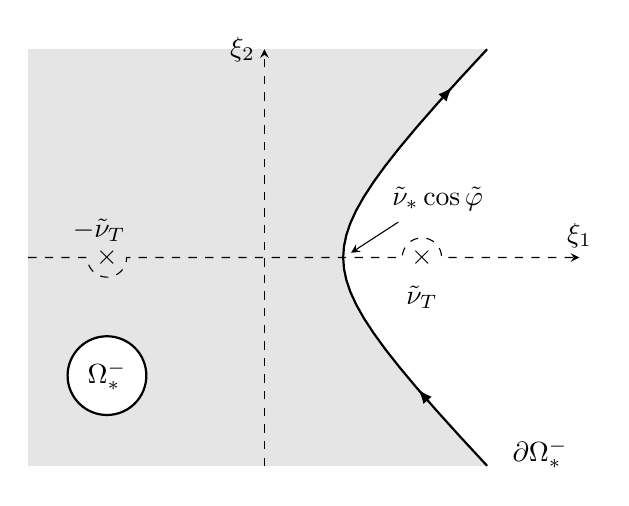
\begin{tikzpicture}
	% Filling Omega_*^-
	\fill [color=gray!20]
	(-3,{-sinh(1.7)})
	-- plot [domain= -1.7:1.7] ({cosh(\x)},{sinh(\x)})
	-- (-3,{sinh(1.7)});
	
%	\fill [color=gray!20]
%	({cosh(1.7)},{-sinh(1.7)})
%	-- plot [domain= 0:-3] ({\x},{-sinh(1.7)})
%	-- (-3,0)
%	-- cycle;
	
%	\fill[color=white] (-2,0) circle (0.25);
	
	\draw[dashed, ->,>=stealth] (-3,0)  -- (-2.25,0) arc(-180:0:0.25)--(1.75,0) arc (180:0:0.25)--(4,0) node[above]{$\xi_1$};
	\draw[dashed, ->,>=stealth](0,{-sinh(1.7)})--(0,{sinh(1.7)}) node[left]{$\xi_2$};
	\node at (2,0) { $\times$}; 
%	\node at (0,1.5) { $\times$}; 
	\node at (2,-0.5) {$\nuti_T$};
%	\node at (0.5,1.5) {$\nuti_L$};
	\node at (-2,0) { $\times$};
%	\node at (0,-1.5) { $\times$}; 
	\node at (-2.1,0.35) {$-\nuti_T$};
%	\node at (-0.5,-1.5) {$-\nuti_L$};
	
	% Hyperbola (contour  partial_Omega_0 )
	\draw[black, thick,decoration={ markings,  % This schema allows for fine-tuning the positions of arrows 
		mark=at position 0.2 with {\arrow{latex}},
		mark=at position 0.9 with {\arrow{latex}}},
	postaction={decorate}][domain=-1.7:1.7] plot({cosh(\x)}, {sinh(\x)});
	
	\node at (3.5,-2.5) {$\partial \Omega_*^-$};
	\draw[thin, ->,>=stealth](1.7,0.45) -- (1.1, 0.06);
	\node at (2.2, 0.75) { $\nuti_*\cos \tilde{\varphi}$};

	% Espace Omega_0
\fill [color=white] (-2,-1.5) circle (0.5);
\draw[thick] (-2,-1.5) circle (0.5);
\node at (-2,-1.5) {$\Omega_*^-$};
	\end{tikzpicture}
	\caption{Domain $\Omega_*^-$ and contour $\partial\Omega_*^-$ in the case $\noncr$.}
	%\label{C4:Omegamoinsnoncr}
	\end{subfigure}
	\hfill
	\begin{subfigure}[b]{0.45\textwidth}
	    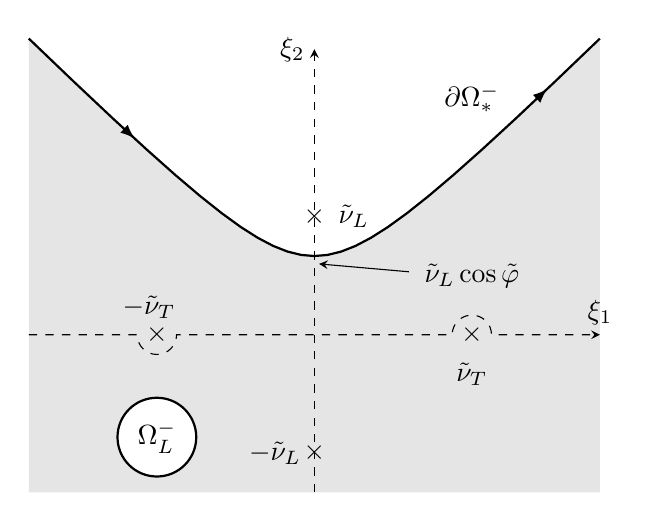
\begin{tikzpicture}
	    	% Filling Omega_*^-
	\fill [color=gray!20]
	({-sinh(2)},-2)
	-- plot [domain= -2:2] ({sinh(\x)},{cosh(\x)})
	--({sinh(2)},-2);

	\draw[dashed, ->,>=stealth] (-3.6269,0)  -- (-2.25,0) arc(-180:0:0.25)--(1.75,0) arc (180:0:0.25)--(3.6269,0) node[above]{$\xi_1$};
	
	\draw[dashed, ->,>=stealth](0,-2)--(0,{sinh(2)}) node[left]{$\xi_2$};
	\node at (2,0) { $\times$}; 
	\node at (0,1.5) { $\times$}; 
	\node at (2,-0.5) {$\nuti_T$};
	\node at (0.5,1.5) {$\nuti_L$};
	\node at (-2,0) { $\times$};
	\node at (0,-1.5) { $\times$}; 
	\node at (-2.1,0.35) {$-\nuti_T$};
	\node at (-0.5,-1.5) {$-\nuti_L$};
	
	% Hyperbola (contour  partial_Omega_0 )
	\draw[black, thick,decoration={ markings,
		mark=at position 0.2 with {\arrow{latex}},
		mark=at position 0.9 with {\arrow{latex}}},
	postaction={decorate}][domain=-2:2] plot({sinh(\x)},{cosh(\x)});
	
	\node at (2,3) {$\partial \Omega_*^-$};
	\draw[thin, ->,>=stealth](1.2,0.8) -- (0.06,0.9);
	\node at (2, 0.75) { $\nuti_L\cos \tilde{\varphi}$};

	% Espace Omega_0
\fill [color=white] (-2,-1.3) circle (0.5);
\draw[thick] (-2,-1.3) circle (0.5);
\node at (-2,-1.3) {$\Omega_L^-$};

	    \end{tikzpicture}
	    %\label{C4:OmegamoinsL}
	    \caption{Domain $\Omega_L^-$ and contour $\partial\Omega_L^-$ in the case $\crit$.}
	\end{subfigure}
\caption{Domains $\Omega_*^-$ and contours $\partial \Omega_*^-$ in cases $\noncr$ and $\crit$.}
\label{C4:dOmegamoins}
\end{figure}

The recursive system of functional equations solved by the regular part is obtained by substituting \eqref{C4:DM2} and \eqref{C4:TM2} into \eqref{C4:regparteqn}:
\begin{equation}
\left\{
\begin{matrix}
X_1(\xi) =g_1(\xi)-\textbf{dm}^{-1}(\xi).\underset{*=L,T}{\sum} \mathbf{M}_*(\xi).X_2(T_*^{-1}(\xi))\textbf{1}_{\Omega_*^-}(\xi) \\
X_2(\xi) =g_2(\xi)-\textbf{dm}^{-1}(\xi).\underset{*=L,T}{\sum} \mathbf{M}_*(\xi).X_1(T_*^{-1}(\xi))\textbf{1}_{\Omega_*^-}(\xi)
\end{matrix}
\right.,
\label{C4:recur}
\end{equation}
where , for $j=1,2$
\begin{equation}
g_j(\xi)=\textbf{dm}^{-1}(\xi)\left( u_j(\xi)- \int_{\Gamma_2}  \textbf{DM}(\xi,\zeta)X_j(\zeta)\, d\zeta- \int_{\partial \Omega_*^-}  \textbf{TM}(\xi,\zeta)X_{3-j}(\zeta)\, d\zeta \right) 
\label{C4:g1g2}
\end{equation}
The same consideration as those made in \ref{C3:propag} lead to an expression of functions $g_j$ using operators $\mathbb{D}(\cdot,\cdot)$ and $\mathbb{T}(\cdot,\cdot)$ :
\begin{equation}
\textbf{dm}(\xi).g_j(\xi)=u_j(\xi)-\sum_{k=1}^{2N} \sqrt{\frac{a_k}{\pi}}\left( \mathbb{ND}(a_k,\xi).\tilde{X}_j^k+\mathbb{NT}(a_k,\xi).\tilde{X}_{3-j}^k \right) ,
\label{C4:gjfinal}
\end{equation}
where
\begin{equation}
\mathbb{ND}(a,b)=\frac{1}{2\pi}\mathbb{D}(a,b)-\frac{\textbf{dm}(b)}{a+b}
\label{C4:defND}
\end{equation}
and
\begin{equation}
\mathbb{NT}(a,b)=\frac{1}{2i\pi}\mathbb{T}(a,b)-\sum_{*=L,T}\frac{\mathbf{M}_*(b)}{T^{-1}_*(b)+a} .
\end{equation}

In system \eqref{C4:recur}, the value of the regular part of the spectral function in domain $\Omega_*^-$, visible Fig.~\ref{C4:dOmegamoins}, is expressed using its value in the domain $\xi \notin \Omega_*^-$, where the numerical approximation \eqref{C4:Xj} is valid. To do so, functions $g_j,\, j=1,2$ are evaluated using \eqref{C4:gjfinal}. The accuracy of the numerical evaluation in domain $\xi \notin \Omega_*^-$ is therefore propagated to domain $\Omega_*^-$. 

This concludes the semi-analytical computation of the spectral functions. Numerical testing is presented in the following.

\section{Numerical Tests}
The L, TH and TV diffraction coefficients are computed using \eqref{C4:Dbeta}. The spectral functions are evaluated in $\xi=\nu_*\cos\theta -i10^{-8}$ (a small negative imaginary part is added to ensure that the recursive equations \eqref{C4:recur} are valid). This is achieved by, first, computing the poles and residues of the spectral functions analytically using the recursive algorithm described in subsection \ref{C4:singpart}. Then, the regular parts of the spectral functions are approached numerically by solving \eqref{C4:regparteqn} thanks to the Galerkin collocation method described in subsection \ref{C4:regpart}, where the Galerkin parameters are set to:
\begin{equation}
a_k=1.001+0.05e^{k\frac{\log 10}{4}}-1, \hspace{3em} b_k=a_k-0.1i, \hspace{3em} 1\leq k\leq20
\end{equation}
Finally, the solution is rendered accurate in the entire complex domain by applying the recursive procedure called the propagation of the solution described in subsection \ref{C4:propag}.

Following these steps, the diffraction coefficients have been computed and tested numerically.

\subsection{Comparison to 2D code}
The first test that has been made on the 3D code is to check that when $\delta_{inc}=0$, the results of the 3D code are the same as those of the 2D code presented in the previous chapter. This has been checked for the theoretical computations and must also be verified numerically (to ensure that no mistakes were made in the code).

\subsection{Verification of the regular part for an infinite plane}
In the case where $\varphi=\pi$, the wedge degenerates into an infinite plane and there is no diffracted wave. The regular part of the spectral functions, which is the part of the solution corresponding to the diffraction phenomena vanishes and we have, for $j=1,2$ :
\begin{equation}
||\mathbb{U}_j||=0 \hspace{1em} \rm and \hspace{1em} ||\mathbb{X}_j||=0
\end{equation}
Verifying that this is the case provides a check on the lengthy computations of the explicit expressions of operators $\mathbb{D}(\cdot,\cdot)$ and $\mathbb{T}(\cdot,\cdot)$.

\subsection{Acoustic limit}
In the second chapter of this manuscript, we have seen that Sommerfeld \cite{Sommerfeld} provides an analytical expression for the \acrshort{gtd} diffraction coefficient in the case of an acoustic wave incident on a wedge with Dirichlet or Neumann boundaries. This is still true for 3D incidences, and the expression is provided by Keller \cite{GTD}. In the case of a wedge with Dirichlet boundaries, we have :
\begin{equation}
\begin{split}
D^{(Dir)}(\theta)=\dfrac{e^{i\dfrac{\pi}{4}}}{2N\sin\delta_{\beta}\sqrt{2\pi}} &\left[ \cot\left(\dfrac{\pi+\theta+\theta_{inc}}{2N} \right) +\cot\left(\dfrac{\pi-\theta-\theta_{inc}}{2N} \right) \right.\\
-&\left. \cot\left(\dfrac{\pi+\theta-\theta_{inc}}{2N} \right)-\cot\left(\dfrac{\pi-\theta+\theta_{inc}}{2N} \right)\right]
\end{split}
\end{equation}

The case of an acoustic wave incident on a wedge with Dirichlet boundary conditions can be mimicked using the elastic code. By setting $c_L=1$ and $c_T \rightarrow 0$ and considering incident L waves, the L diffraction coefficient behaves like the diffraction coefficient of an acoustic wave. Comparing our results to Sommerfeld's analytical formulation, provides an additional check on the results.

\subsection{Case where $\crit$}
In the case where $\crit$, the code developed according to the theory described in this chapter produces diverging results. Additional work is necessary in order to solve this problem. In the meantime, in order to obtain coherent results, the following approximation is applied :
\begin{equation}
X_j|_{\delta_{\beta}>\delta_C} \approx X_j|_{\delta_{\beta}=\delta_C-\epsilon}
\end{equation}

\section*{Conclusion}
Using the spectral functions method, the elastic wave diffracted by a skew incident plane wave on as stress-free wedge has been studied. In cases where Snell's law of diffraction has a solution for both longitudinal and transversal diffracted waves, a semi-analytical computation method is developed theoretically and numerically. The corresponding code has been checked in three different manners, yielding promising results. In the case of an incident transversal wave, with a skew angle higher than the critical angle in diffraction, Snell's law of diffraction leads only to transversal diffracted waves. This case is also treated theoretically but the corresponding numerical code produces diverging results. Further investigations are necessary in order to solve this problem. In the meantime, an approximate solution is proposed, in order to obtain a less exact, yet physically meaningful result. This approximate solution still remains to be tested.

%
% Chapitre  de conclusion (générale)
%%%%%%%%%%%%%%%%%%%%%%%%%%%%%%%%%%%%%%%%%%%%%%%%%%%%%%%%%%%%%%%%%%%%%%%%%%%%%%%
\chapter*{Conclusion}

The aim of this thesis is to propose and validate a generic and reliable elastodynamic wedge-diffraction model, valid for all wedge angles and for 3D incidences. So far, this had not yet been done in elastodynamics. This is done by extending a method called the \acrfull{sf} method and proposing the corresponding numerical resolution schemes. The principal results of this thesis are summarized in the following.



The results obtained during this thesis led to two publications in peer-reviewed journals \cite{article, articleelasto} as well to two communications in international conferences with conference proceedings \cite{DD2018,AFPAC}.

Some suggestions for future work are given below :
\begin{itemize}
\item In the final chapter of this thesis, the regular part of the spectral functions diverges in certain cases. Further investigations need to be made in order to find the cause of these divergences and a new method of computation needs to be proposed.
\item A thorough numerical and/or experimental validation of the code implemented to treat the case of 3D diffraction of an elastic wave must be conducted.
\item The \acrlong{sf} method could be further extended to treat dihedral interfaces between two elastic materials. This would be the continuity of Lucien Rochery's internship.
\item The \acrshort{utd} model was developed by Audrey Kamta-Djakou \cite{AKDthese} using the \acrfull{si} pole propagation algorithm. It should be adapted to the \acrshort{sf} method so it can be applied to 3D incidences.
\item The elastodynamic diffraction coefficients present a slight discontinuity at critical angles, due to the presence of head waves. In the continuity of Fradkin et al. \cite{FradkinDarmon}, further investigations must be made in order to model the contribution of these waves correctly.
\item In the final chapter, it was shown that for transversal incident waves with a skew angle higher than the critical angle, an evanescent longitudinal wave is produced. The asymptotic contribution of this wave should be evaluated more precisely.
\item Following the ideas of Kamotskii \cite{Kamotski2}, the Spectral Functions method could also be adapted to treat scattering by multiple adjacent wedges.
\end{itemize}
%
%%%%%%%%%%%%%%%%%%%%%%%%%%%%%%%%%%%%%%%%%%%%%%%%%%%%%%%%%%%%%%%%%%%%%%%%%%%%%%%
% Début de la partie annexe éventuelle
%%%%%%%%%%%%%%%%%%%%%%%%%%%%%%%%%%%%%%%%%%%%%%%%%%%%%%%%%%%%%%%%%%%%%%%%%%%%%%%
\appendix

\chapter{Steepest Descent Method}
\label{PhaseStationnaire}
The steepest descent method is an integral approximation technique where the integration contour is deformed into a contour $\gamma$ called the steepest descent contour, which passes near a saddle-point of the integrated function. The method was first published by Debye \cite{Debye} but the ideas were first suggested by Riemann in an unpublished note \cite{RiemannUnpub}, which was printed later \cite{Riemann}. A description of the method can be found in English in the translated version of the Encyclopedia of Mathematics \cite{Encycl}. Useful results are stated here without demonstration.

\paragraph{}
The integral to be estimated is of the form :
\begin{equation}
I(\lambda)=\int_C f(z)e^{\lambda S(z)}\,dz
\end{equation}
where $C$ is the integration contour, $S$ and $f$ are analytical on all $\mathbb{C}^n$, except for eventually at a finite number of points, and $\lambda>0$. The steepest descent contour $\gamma$ must verify :
\begin{itemize}
\item $C$ and $\gamma$ must have the same endpoints,
\item $\gamma$ passes through at least one saddle point of $S$,
\item Im$(S(z))$ is constant on $\gamma$.
\end{itemize}

\paragraph{}
Le us denote $\mathbf{S_{xx}}(z)$ the hessian matrix of $S$, defined by :
\begin{equation}
\mathbf{S_{xx}}(z)=\left( \frac{\partial^2 S}{\partial x_i \partial x_j}(z) \right)_{1\leq i,j \leq n},
\end{equation}
then $z_ 0$ is a non-degenerate saddle point of $S$ if and only if :
\begin{eqnarray}
\left\{
\begin{array}{l}
\nabla S(z_0)=0 \\
\mbox{det} \; \mathbf{S_{xx}}(z_0) \neq 0
\end{array}
\right.
\end{eqnarray}

The following proposition is then true :

\begin{prop}
Assume
\begin{description}
  \item[(i)] $f$ and $S$ are holomorphic on an open, bounded and simply connected subset $W_x \subset \mathbb{C}^n$ such that $I_x=W_x \cap \mathbb{R}^n$ is connected,
  \item[(ii)]$ Re\left( S(z) \right)$ has a single maximum reached at exactly one point $z_0 \in I_x$,
  \item[(iii)] $z_0$ is a non-degenerate saddle point of $S$.
\end{description}
The following asymptotic evaluation then holds :
\begin{equation}
I(\lambda) \underset{\lambda \to +\infty}{=} \left( \frac{2\pi}{\lambda} \right)^{n/2} e^{\lambda S(z_0)} \lbrack f(z_0)+ \mathcal{O}(\lambda^{-1}) \rbrack \prod_{j=1}^n (-\mu_j)^{-1/2},
\label{steepformula}
\end{equation}
where $(\mu_j)_{1\leq j \leq n}$ are the eigen values of $\mathbf{S_{xx}}(z_0)$ and their square roots are defined by
$$|\mbox{arg} \sqrt{-\mu_j}| <\frac{\pi}{4} $$
\end{prop}

Note that any if any singularities are crossed during deformation of contour $C$ to contour $\gamma$, their contribution to the integral must be correctly taken into account.

\chapter{Calcul des intégrales $\int_{-1}^1 \frac{\lambda t+ \rho}{Q(t)}\, dt$ et $\int_{-1}^1 \frac{\eta t+ \psi}{P(t)}\, dt$ }
\label{Intégrale}
Avant de nous lancer dans le détail des calculs des coefficients des matrices $\mathbb{D}$ et $\mathbb{T}$, nous allons commencer par calculer deux intégrales élémentaires dont les valeurs seront utilisées dans toute la suite.
\section{Intégrale $\int_{-1}^1 \frac{\lambda t+ \rho}{Q(t)}\, dt$}
\label{calculIntQ}
On calcule :
\begin{equation*}
\int_{-1}^1 \frac{\lambda t+ \rho}{Q(t)}\, dt=\int_{-1}^1 \frac{\lambda t}{iat^2+2\nu t-ia}\,dt+\int_{-1}^1\frac{\rho}{ia(t-q_+)(t-q_-)}\,dt
\end{equation*}
Où on note $q_+,q_-$ les racines de Q. On a:
\begin{equation}
q_\pm=\frac{1}{a}(i\nu\pm\sqrt{a^2-\nu^2})
\label{q1q2}
\end{equation}

\begin{equation*}
\begin{split}
\int_{-1}^1 \frac{\lambda t+ \rho}{Q(t)}\, dt&=\int_{-1}^1 \frac{\frac{\lambda}{2ia} (2iat+2\nu)}{iat^2+2\nu t-ia}\,dt+(\rho-\frac{\lambda \nu}{ia})\int_{-1}^1\frac{1}{ia(t-q_+)(t-q_-)}\,dt\\
&=\frac{\lambda\pi}{2a}+\frac{1}{q_+-q_-}\left(\frac{\rho}{ia}+\frac{\lambda\nu}{a^2}\right)\int_{-1}^1\left(\frac{1}{t-q_+}-\frac{1}{t-q_-}\right)\,dt
\end{split}
\end{equation*}
On réinjecte les expressions de $q_\pm$ données par (\ref{q1q2}):
\begin{equation*}
\begin{split}
\int_{-1}^1 \frac{\lambda t+ \rho}{Q(t)}\, dt&=\frac{\lambda\pi}{2a}+\frac{1}{2\sqrt{a^2-\nu^2}}\left(\frac{\lambda\nu}{a}-i\rho\right)\log\left(\frac{(1-q_+)(1+q_-)}{(1-q_-)(1+q_+)}\right)\\
&=\frac{\lambda\pi}{2a}+\frac{1}{2\sqrt{a^2-\nu^2}}\left(\frac{\lambda\nu}{a}-i\rho\right)\log\left(\frac{-\nu^2-(a-\sqrt{a^2-\nu^2})^2}{-\nu^2-(a+\sqrt{a^2-\nu^2})^2}\right)\\
&=\frac{\lambda\pi}{2a}+\frac{1}{2\sqrt{a^2-\nu^2}}\left(\frac{\lambda\nu}{a}-i\rho\right)\log\left(\frac{-a+\sqrt{a^2-\nu^2}}{-a-\sqrt{a^2-\nu^2}}\right)\\
&=\frac{\lambda\pi}{2a}+\frac{1}{\nu\sqrt{\frac{a^2}{\nu^2}-1}}\left(i\rho-\frac{\lambda\nu}{a}\right)\log\left(\frac{a}{\nu}+\sqrt{\frac{a^2}{\nu^2}-1}\right)
\end{split}
\end{equation*}
Soit finalement :
\begin{equation}
\int_{-1}^1 \frac{\lambda t+ \rho}{Q(t)}\, dt=\frac{\lambda}{\nu}\mbox{sog}(\frac{a}{\nu})+i\frac{\rho}{\nu}\mbox{rog}(\frac{a}{\nu})
\label{intQ}
\end{equation}
On a défini la fonction suivante, pour $a>1$
\begin{equation}
\mbox{rog}(a)=\int_{-1}^1\frac{dx}{a(1-x^2)+2ix}=\frac{1}{\sqrt{a^2-1}}\log(a+\sqrt{a^2-1})
\label{defrog}
\end{equation}
La branche de coupure de la racine carrée est le long de l'axe des réels négatifs. On definit ensuite :
\begin{equation}
\mbox{sog}(a)=\frac{1}{a}\left(\frac{\pi}{2}-\mbox{rog}(a)\right)
\label{defsog}
\end{equation}
\section{Intégrale $\int_{-1}^1 \frac{\eta t+ \psi}{P(t)}\, dt$}
\label{calculintP}
On calcule :
\begin{equation*}
\int_{-1}^1 \frac{\eta t+ \psi}{P(t)}\, dt = \int_{-1}^1 \frac{\eta t}{(\nu\sin\tilde{\varphi}-b)t^2-2i\nu t\cos\tilde{\varphi}+\nu\sin\tilde{\varphi}+b}\,dt +\int_{-1}^1 \frac{\psi}{(\nu\sin\tilde{\varphi}-b)(t-p_+)(t-p_-)}\, dt
\end{equation*}
Où on note $p_+,p_-$ les racines de $P$. On a :
\begin{equation}
p_\pm=\frac{\nu i \cos\tilde{\varphi}\pm \sqrt{b^2-\nu^2}}{\nu\sin\varphi-b}
\label{p1p2}
\end{equation}
\begin{equation*}
\begin{split}
\int_{-1}^1 \frac{\eta t+ \psi}{P(t)}\, dt =& \int_{-1}^1 \frac{\frac{\eta}{2(\nu\sin\tilde{\varphi}-b)}(2(\nu\sin\tilde{\varphi}-b)t-2i\nu\cos\tilde{\varphi})}{(\nu\sin\tilde{\varphi}-b)t^2-2i\nu t\cos\tilde{\varphi}+\nu\sin\tilde{\varphi}+b}\,dt\\
&+(\psi+\frac{\eta i\nu\cos\tilde{\varphi}}{\nu\sin\tilde{\varphi}-b})\int_{-1}^1 \frac{dt}{(\nu\sin\tilde{\varphi}-b)(t-p_+)(t-p_-)}\\
=&\frac{i\eta}{\nu\sin\tilde{\varphi}-b}(\tilde{\varphi}-\frac{\pi}{2})\\
&+\frac{1}{p_+-p_-}\left(\frac{\psi}{\nu\sin\tilde{\varphi}-b}+\frac{\eta i\nu\cos\tilde{\varphi}}{(\nu\sin\tilde{\varphi}-b)^2}\right)\int_{-1}^1 \left(\frac{1}{t-p_+}-\frac{1}{t-p_-}\right)\,dt\\
\end{split}
\end{equation*}
On réinjecte les expressions de $p_\pm$ données par (\ref{p1p2}) :
\begin{equation*}
\begin{split}
\int_{-1}^1 \frac{\eta t+ \psi}{P(t)}\, dt =&\frac{i\eta}{\nu\sin\tilde{\varphi}-b}(\tilde{\varphi}-\frac{\pi}{2})+\frac{1}{2\sqrt{b^2-\nu^2}}\left(\psi+\frac{\eta i\nu\cos\tilde{\varphi}}{\nu\sin\tilde{\varphi}-b}\right)\log\left(\frac{(1-p_+)(1+p_-)}{(1-p_-)(1+p_+)}\right)\\
=&\frac{i\eta}{\nu\sin\tilde{\varphi}-b}(\tilde{\varphi}-\frac{\pi}{2})\\
&+\frac{1}{2\sqrt{b^2-\nu^2}}\left(\psi+\frac{\eta i\nu\cos\tilde{\varphi}}{\nu\sin\tilde{\varphi}-b}\right)\log\left(\frac{-\nu^2\cos^2\tilde{\varphi}-(\nu\sin\tilde{\varphi}-b-\sqrt{b^2-\nu^2})^2}{-\nu^2\cos^2\tilde{\varphi}-(\nu\sin\tilde{\varphi}-b+\sqrt{b^2-\nu^2})^2}\right)\\
=&\frac{i\eta}{\nu\sin\tilde{\varphi}-b}(\tilde{\varphi}-\frac{\pi}{2})+\frac{1}{2\sqrt{b^2-\nu^2}}\left(\psi+\frac{\eta i\nu\cos\tilde{\varphi}}{\nu\sin\tilde{\varphi}-b}\right)\log\left(\frac{b+\sqrt{b^2-\nu^2}}{b-\sqrt{b^2-\nu^2}}\right)\\
=&\frac{i\eta}{\nu\sin\tilde{\varphi}-b}(\tilde{\varphi}-\frac{\pi}{2})+\frac{1}{\nu\sqrt{\frac{b^2}{\nu^2}-1}}\left(\psi+\frac{\eta i\nu\cos\tilde{\varphi}}{\nu\sin\tilde{\varphi}-b}\right)\log\left(\frac{b}{\nu}+\sqrt{\frac{b^2}{\nu^2}-1}\right)
\end{split}
\end{equation*}
Finalement :
\begin{equation}
\int_{-1}^1 \frac{\eta t+ \psi}{P(t)}\, dt =\frac{i\eta}{\nu\sin\tilde{\varphi}-b}\lbrack\tilde{\varphi}-\frac{\pi}{2}+\cos\tilde{\varphi} \mbox{rog}(\frac{b}{\nu})\rbrack+\frac{\psi}{\nu}\mbox{rog}(\frac{b}{\nu})
\label{intP}
\end{equation}

\chapter{Computation details for the coefficients of matrix $\mathbb{D}(a,b)$}
\label{matD}
In each chapter of this manuscript, a matrix $\mathbb{D}$ appears, the coefficients of which must be determined analytically. These coefficients are linear combinations of integrals noted $I_1^*$ to $I_5^*$. In this appendix, these integrals are defined and the details of their computation is given. Finally, expressions of the coefficients of matrix $\mathbb{D}$ in the acoustic and 2D and 3D elastic cases are given. In all the following, $\nuti \in \{ 1,\nu_T,\nuti_L,\nuti_T \}$.

\section{Integral $I_1^*$}
\label{calcI1}
Integral $I_1^*$ is defined by :
\begin{equation}
\label{defI1}
I_1^*=\int_{-\infty}^{+\infty} \frac{y}{(y+ib)(y-ia)\sqrt{\nuti^2+y^2}}\,dy
\end{equation}
When $a+b \neq 0$, we have the simple elements decomposition :
\begin{equation}
\frac{y}{(y+ib)(y-ia)}=\frac{1}{a+b} \left( \frac{b}{y+ib}+\frac{a}{y-ia} \right), 
\label{decomp2}
\end{equation}
which leads to
\begin{equation}
I_1^*= \frac{1}{a+b} \left( \int_{-\infty}^{+\infty} \frac{b}{(y+ib)\sqrt{\nuti^2+y^2}} \,dy +\int_{-\infty}^{+\infty} \frac{a}{(y-ia)\sqrt{\nuti^2+y^2}} \,dy \right)
\end{equation}
In each of these integrals, the following variable change is applied :
\begin{equation}
\begin{split}
 y&=2\nuti \frac{t}{1-t^2} \\
\sqrt{\nuti^2+y^2}&=\nuti\left( \frac{1+t^2}{1-t^2} \right)  \\
 dy&= 2\nuti \frac{1+t^2}{(1-t^2)^2}dt 
\end{split}
\label{changevar}
\end{equation}
Yielding
\begin{equation}
\int_{-\infty}^{+\infty} \frac{dy}{(y-ia)\sqrt{\nuti^2+y^2}}=\int_{-1}^1\frac{2\,dt}{2\nuti t-ia(1-t^2)}
\end{equation}
Finally, formula \eqref{intQ} is applied :
\begin{equation}
I_1^*=\frac{2ia}{(a+b)\nuti}\mbox{rog}(a/\nuti)-\frac{2ib}{(a+b)\nuti}\mbox{rog}(b/\nuti)
\label{valI1}
\end{equation}

\section{Integral $I_2^*$}
\label{calcI2}
Integral $I_2^*$ is defined by :
\begin{equation}
I_2^*=  \int_{-\infty}^{+\infty} \frac{y\sqrt{\nuti^2+y^2}}{(y+ib)(y-ia)}\, dy
\label{defI2}
\end{equation}
Note that
\begin{equation*}
\begin{split}
I_2^*&=\nuti^2 \int_{-\infty}^{+\infty}  \frac{y}{(y+ib)(y-ia)\sqrt{\nuti^2+y^2}}\,dy+ \int_{-\infty}^{+\infty} \frac{y^3}{(y+ib)(y-ia)\sqrt{\nuti^2+y^2}} \, dy\\
I_2^*&=\nuti^2 I_1^*+I_3^*,
\end{split}
\end{equation*}
where integrals $I_1^*$ and $I_3^*$ are defined by equations \eqref{defI1} and \eqref{defI3} and their expressions are given by \eqref{valI1} and \eqref{valI3} respectively.

\section{Integral $I_3^*$}
\label{calcI3}
Integral $I_3^*$ is defined by :
\begin{equation}
I_3^*=\int_{-\infty}^{+\infty} \frac{y^3}{(y+ib)(y-ia)\sqrt{\nuti^2+y^2}} \,dy
\label{defI3}
\end{equation}
The simple elements decomposition \eqref{decomp2} leads to
\begin{equation}
I_3^*=\frac{b}{a+b}\int_{-\infty}^{+\infty} \frac{y^2}{(y+ib)\sqrt{\nuti^2+y^2}} \, dy +\frac{a}{a+b}\int_{-\infty}^{+\infty} \frac{y^2}{(y-ia)\sqrt{\nuti^2+y^2}} \, dy
\label{decompI3}
\end{equation}

Once again, variable change \eqref{changevar} is applied
\begin{equation}
 \int_{-\infty}^{+\infty} \frac{y^2}{(y-ia)\sqrt{\nuti^2+y^2}} \,dy = \int_{-1}^1 \frac{8\nuti^2t^2}{(1-t^2)^2(2\nuti t -ia(1-t^2))} \, dt
\end{equation}

The integrated functions can be decomposed as such :
\begin{equation}
\frac{t^2}{(1-t^2)^2(2\nuti t -ia(1-t^2))}=\frac{\alpha}{1-t}+\frac{\beta}{1+t}+ \frac{\gamma}{(1-t)^2}+\frac{\delta}{(1+t)^2} +\frac{\lambda t + \rho }{2\nuti t-ia(1-t^2)},
\label{elemsimpl3}
\end{equation}
where the coefficients $\alpha,\beta,\gamma,\delta,\lambda,\rho$ will be determined in the sequel.

To determine $\gamma$, \eqref{elemsimpl3} is multiplied by $(1-t)^2$ and the result is evaluated at $t=1$. Similarly, $\delta$ is determined by multiplying \eqref{elemsimpl3} by $(1+t)^2$ and evaluating the result at $t=-1$ :
\begin{subequations}
\begin{equation}
\gamma=\frac{1}{8\nuti}
\end{equation}
\begin{equation}
\delta = -\frac{1}{8\nuti}
\end{equation}
\end{subequations}

The remaining terms are
\begin{equation}
\begin{split}
\frac{\alpha}{1-t}+\frac{\beta}{1+t}&+ \frac{\lambda t + \rho }{2\nuti t-ia(1-t^2)}\\  
~\\
&=\frac{t^2}{(1-t^2)^2(2\nuti t -ia(1-t^2))}-\frac{1}{8\nuti(1-t)^2}+\frac{1}{8\nuti(1+t)^2}  \\
~\\
&=\frac{8\nuti t^2-(1+t)^2(2\nuti t-ia(1-t^2))+(1-t)^2(2\nuti t-ia(1-t^2))}{8\nuti(1-t^2)^2(2\nuti_*-ia(1-t^2))}\\
~\\
&=\frac{iat}{2\nuti(1-t^2)(2\nuti t-ia(1-t^2))}
\end{split}
\end{equation}

To determine $\alpha$, \eqref{elemsimpl3} is multiplied by $(1-t)$ and the result is evaluated at $t=1$. Similarly, $\beta$ is determined by multiplying \eqref{elemsimpl3} by $(1+t)$ and evaluating the result at $t=-1$ :
\begin{subequations}
\begin{equation}
\alpha=\frac{ia}{8\nuti^2}
\end{equation}
\begin{equation}
\beta=\frac{ia}{8\nuti^2}
\end{equation}
\end{subequations}

The remaining term is
\begin{equation}
\begin{split}
 \frac{\lambda t + \rho }{2\nuti t-ia(1-t^2)} &=\frac{iat}{2\nuti(1-t^2)(2\nuti-ia(1-t^2))} -\frac{ia}{8\nuti^2(1-t)}-\frac{ia}{8\nuti^2(1+t)} \\
&= \frac{2\nuti iat-ia(2\nuti t-ia(1-t^2))}{4\nuti^2(1-t^2)(2\nuti t-ia(1-t^2))} \\
&=\frac{-a^2}{4\nuti ^2(2\nuti t-ia(1-t^2))}
\end{split}
\end{equation}
The final coefficients can now be determined by a simple identification :
\begin{subequations}
\begin{equation}
\lambda=0
\end{equation}
\begin{equation}
\rho=-\frac{a^2}{4\nuti^2}
\end{equation}
\end{subequations}

Finally, equation \eqref{intQ} can be applied :
\begin{equation}
\int_{-\infty}^{+\infty} \frac{y^2}{(y-ia)\sqrt{\nuti^2+y^2}} \, dy =2ia\log\left(\frac{1+t_{\nuti}}{1-t_{\nuti}}\right)-2i\frac{a^2}{\nuti}\rog{\frac{a}{\nuti}}
\label{y2_D}
\end{equation}
The value of $\int_{-\infty}^{+\infty} \dfrac{y^2}{(y+ib)\sqrt{\nuti^2+y^2}} \, dy $ can be obtained by taking the complex conjugate of  $\int_{-\infty}^{+\infty} \dfrac{y^2}{(y-ia)\sqrt{\nuti^2+y^2}} \, dy $ replacing $a$ with $b$ in the result. The final result can then be obtained using \eqref{decompI3} :
\begin{equation}
\begin{split}
I_3^*&=i(a-b)\int_{-1}^1 \left( \frac{1}{1-t}+\frac{1}{1+t} \right) \, dt+ 2\nuti \int_{-1}^1 \left( \frac{1}{(1-t)^2}-\frac{1}{(1+t)^2} \right) \, dt \\
 &-\frac{2a^3}{a+b}\int_{-1}^1\frac{dt}{2\nuti t-ia(1-t^2)}-\frac{2b^3}{a+b}\int_{-1}^1\frac{dt}{2\nuti t+ib(1-t^2)}\\
 ~\\
 &=2i(a-b)\log\left(\frac{1+t_{\nuti}}{1-t_{\nuti}}\right)-\frac{2ia^3}{\nuti(a+b)}\mbox{rog}(a/\nuti)+\frac{2ib^3}{\nuti(a+b)}\mbox{rog}(b/\nuti) 
\end{split}
\label{valI3}
\end{equation}
Note the appearance of the diverging term $\log\left(\dfrac{1+t_{\nuti}}{1-t_{\nuti}}\right)$. This term will be compensated by another in the final expression of the coefficients of matrix $\mathbb{D}$. In fact, \eqref{changevar} leads to :
\begin{equation}
\frac{2t_{\nuti}}{1-t_{\nuti}^2}=\frac{A}{\nuti} \mbox{ and } A\rightarrow + \infty \mbox{ when } t_{\nuti} \rightarrow 1
\end{equation}
and
\begin{equation}
1-t_{\nuti} =\frac{(1-t_{\nuti})(1+t_{\nuti})}{1+t_{\nuti}} \sim \frac{\nuti}{A}
\end{equation}
so that
\begin{equation}
\ln\left(\frac{1+t_{\nuti_L}}{1-t_{\nuti_L}}\right)- \ln\left(\frac{1+t_{\nuti_T}}{1-t_{\nuti_T}}\right)\sim \ln\left(\frac{\nuti_T}{\nuti_L}\right) 
\label{compensation}
\end{equation}

\section{Integral $I_4^*$}
\label{calcI4}
Integral $I_4^*$ is defined by :
\begin{equation}
I_4^*=\int_{-\infty}^{+\infty} \dfrac{dy}{(y+ib)(y-ia)\sqrt{\nuti^2+y^2}}
\label{defI4}
\end{equation}
For $a+b\neq0$, 
\begin{equation}
    \frac{1}{(y+ib)(y-ia)}=\frac{-i}{a+b}\left( \frac{1}{y-ia}-\frac{1}{y+ib}\right)
    \label{decomp1}
\end{equation}
Substituting the above decomposition in \eqref{defI4}, we get
\begin{equation}
I_4^*=\frac{i}{a+b} \int_{-\infty}^{+\infty} \left(\frac{1}{(y+ib)\sqrt{\nuti^2+y^2}}-\frac{1}{(y-ia)\sqrt{\nuti^2+y^2}} \right)\,dy
\end{equation}
These integrals have been computed in section \ref{calculIntQ}. Using \eqref{intQ}, we get :
\begin{equation}
I_4^*=\frac{2}{\nuti(a+b)}\left(\rog{a/\nuti}+\rog{b/\nuti} \right)
\label{valI4}
\end{equation}

\section{Integral $I_5^*$}
\label{calcI5}

Integral $I_5^*$ is defined by :
\begin{equation}
I_5^*=\int_{-\infty}^{+\infty} \frac{y^2}{(y+ib)(y-ia)\sqrt{\nuti^2+y^2}}\,dy
\end{equation}
Using decomposition \eqref{decomp1} we get
\begin{equation}
I_5^*=\frac{i}{a+b}\int_{-\infty}^{+\infty}\left( \frac{y^2}{(y+ib)\sqrt{\nuti^2+y^2}}-\frac{y^2}{(y-ia)\sqrt{\nuti^2+y^2}}\right)\,dy
\end{equation}
These integrals have been computed at section \ref{calcI3}. Applying formula \eqref{y2_D}, we get :
% En appliquant le changement de variables \eqref{changevar}, on a
% $$\int_{-\infty}^{+\infty}\frac{y}{(y-ia)\sqrt{\nuti_*^2+y^2}} \, dy=\int_{-1}^1 \frac{4\nuti t}{(1-t^2)(2\nuti t-ia(1-t^2))}\,dt$$
% On cherche la décomposition en éléments simples de l'intégrande :
% $$\frac{2\nuti t}{(1-t^2)(2\nuti t-ia(1-t^2)} = \frac{\alpha}{1-t}+\frac{\beta}{1+t}+\frac{\lambda t+\rho}{Q(t)}$$
% On a alors
% $$\alpha=\beta=1$$
% et 
% $$\lambda=0, \, \, \; \rho=2ia$$
% La formule \eqref{intQ} nous donne finalement :
\begin{equation}
I_5^*=2\log\left(\frac{1+t_{\nuti}}{1-t_{\nuti}}\right)-\frac{2}{\nuti(a+b)}\lbrack b^2\rog{b/\nuti}+a^2\rog{a/\nuti}\rbrack
\label{intI5}
\end{equation}

\section{Continuation and conclusion of the computation of the coefficients of $\mathbb{D}(a,b)$}
\label{fincalculs}
The final steps of the computation of the coefficients of matrices $\mathbb{D}_{lk}$ are given here. For each physical configuration presented in this manuscript, the coefficients can be expressed as linear combinations of integrals $I_1^*$ to $I_5^*$. These combinations are given case by case in the following.

\subsection{Acoustic case}
\label{finalDac}
In the second chapter of this manuscript, which deals with the diffraction of an acoustic wave, the expression of operator $\mathcal{D}(a,b)$ depends on whether the wedge is soft (Dirichlet boundary conditions) or hard (Neumann boundary conditions). Let us begin with the case of a soft wedge.  
\subsubsection{Dirichlet boundary conditions}
\label{finalDacDir}
In the case of Dirichlet boundary conditions, the expression of function $\mathcal{D}(a,b)$ is obtained by substituting \eqref{dmDir} in \eqref{ldbis} for $a>1$ and $b>1$ :
\begin{equation}
\mathcal{D}(a,b) = \int_{-\infty}^{+\infty} \dfrac{1}{ y+ib} \, \dfrac{1}{y -i a} \,\dfrac{1}{\zeta_0^0(iy)} \, dy . 
\end{equation}
According to \eqref{zeta_function}, the above expression can be simplified using the relation
\begin{equation}
\zeta_0^0(iy)= - \sqrt{1+y^2}.
\label{zeta0iy}
\end{equation}
By setting $\nuti=1$ in \eqref{defI4}, we find :
\begin{equation}
\mathcal{T}(a,b)=-I_4^1
\end{equation}
This integral is computed in section \ref{calcI4} and its value is given by \eqref{valI4}.
\subsubsection{Neumann boundary conditions}
\label{finalDacNeu}
In the case of Neumann boundary conditions, the expression of function $\mathcal{D}(a,b)$ is obtained by substituting \eqref{dmNeu} in \eqref{ldbis} for $a>1$ and $b>1$ :
\begin{equation}
\mathcal{D}(a,b) = \int_{-\infty}^{+\infty} \dfrac{dy}{ (y+ib)(y-ia)} \, dy .
\end{equation}
The result can be computed directly, by using Cauchy's residue theorem, yielding :
\begin{equation}
\mathcal{D}(a,b)=\dfrac{2\pi}{a+b}
\end{equation}

\subsection{2D elastic case}
\label{finalD2D}
\subsection{3D elastic case}
\label{finalD3D}

\chapter{Computation details for the coefficients of matrix $\mathbb{T}(a,b)$}
\label{matT}
In each chapter of this manuscript, a matrix $\mathbb{T}(a,b)$ appears, the coefficients of which can be determined analytically. These coefficients are linear combinations of integrals $J_1^*$ to $J_8^*$. In this appendix, these integrals are defined and the details of their computation is given. Finally, expressions of the coefficients of matrix $\mathbb{T}(a,b)$ in the acoustic case and 2D and 3D elastic cases are given with respect to integrals $J_1^*$ to $J_8^*$. In all the following, $\nuti \in \{1,\nu_T, \nuti_L,\nuti_T\}$.

\section{Integral $J_1^*$}
\label{calcJ1}
Integral $J_1^*$ is defined by :
\begin{equation}
\begin{split}
J_1^*&= \int_{-\infty}^{+\infty} \frac{y (\nuti^2+y^2)}{(y-ia)\lbrack b-iy\cos \varphi+ \sqrt{\nuti^2+y^2} \sin\phiti) \rbrack\sqrt{\nuti^2+y^2}} \, dy\\
&=\nuti^2J_5^*+J_4^*
\end{split}
\label{defJ1}
\end{equation}
where integral $J_4^*$ and $J_5^*$ are defined by equations \eqref{defJ4} and \eqref{defJ5} and their expressions are given \eqref{valJ4} nad \eqref{valJ5} respectively.

\section{Integral $J_2^*$}
\label{calcJ2}
Integral $J_2^*$ is defined by :
\begin{equation}
J_2 =\int_{-\infty}^{+\infty} \frac{y^2}{(y-ia)\lbrack b-iy\cos \tilde{\varphi}+ \sqrt{\nuti^2+y^2} \sin \tilde{\varphi}) \rbrack} \, dy
\label{defJ2}
\end{equation}
Once again, variable change \eqref{changevar} is applied 
\begin{equation}
J_2=8\nuti^3 \int_{-1}^1 \frac{t^2(t^2+1)}{(1-t^2)^2\lbrack b(1-t^2)-2\nuti it\cos\tilde{\varphi}+ \sin \tilde{\varphi} \nuti(1+t^2)\rbrack(2\nuti t-ia(1-t^2))}\, dt
\end{equation}
We have the following simple elements decomposition :
\begin{equation}
\frac{t^2(1+t^2)}{(1-t)^2(1+t)^2P(t)Q(t)}=\frac{\alpha_2}{1-t}+\frac{\beta_2}{1+t}+\frac{\gamma_2}{(1-t)^2}+\frac{\delta_2}{(1+t)^2}+\frac{\eta_2 t+\psi_2}{P(t)}+\frac{\lambda_2 t +\rho_2}{Q(t)}
\label{decompJ2}
\end{equation}
where the coefficients of the decomposition are determined in the sequel.

The first step is to determine $\gamma_2$ by multiplying the above decomposition by $(1-t)^2$ and evaluating the result at $t=1$. Similarly, $\delta_2$ is determined by multiplying \eqref{decompJ2} by $(1+t)^2$ and evaluating the result at $t=-1$ :
\begin{subequations}
\begin{equation}
\gamma_2=\frac{e^{i(\pi/2-\tilde{\varphi})}}{8\nuti^2}
\end{equation}
\begin{equation}
\delta_2=\frac{e^{i(\pi/2+\tilde{\varphi})}}{8\nuti^2}
\end{equation}
\end{subequations}
The remaining terms are
\begin{equation}
\begin{split}
\frac{\alpha_2}{1-t}&+\frac{\beta_2}{1+t} +\frac{\eta_2 t+\psi_2}{P(t)}+\frac{\lambda_2 t +\rho_2}{Q(t)}=\frac{t^2(1+t^2)}{(1-t)^2(1+t)^2P(t)Q(t)}-\frac{e^{i(\pi/2-\tilde{\varphi})}}{8\nuti^2(1-t)^2}-\frac{e^{i(\pi/2+\tilde{\varphi})}}{8\nuti^2(1+t)^2}\\
&=\frac{2iab\sin\tilde{\varphi}t-\nuti^2i\sin(2\tilde{\varphi})t-ab\cos\tilde{\varphi}(1+t^2)}{4\nuti^2 P(t)Q(t)}\\ &+\frac{(2t\sin\tilde{\varphi}+(1+t^2)i\cos\varphi)(2a\cos\tilde{\varphi}t+ai\sin\tilde{\varphi}(1+t^2)-2bt)}{4\nuti(1-t^2) P(t)Q(t)}
\end{split}
\end{equation}
$\alpha_2$ is determined by multiplying the above decomposition by $(1-t)$ and evaluating the result at $t=1$. Similarly, $\beta_2$ is determined by multiplying the above equation by $(1+t)$ and evaluating the result at $t=-1$ :
\begin{subequations}
\begin{equation}
\alpha_2=\frac{be^{-2i\tilde{\varphi}}-ae^{-i\tilde{\varphi}}}{8\nuti^3}
\end{equation}
\begin{equation}
\beta_2=\frac{ae^{i\tilde{\varphi}}-be^{2i\tilde{\varphi}}}{8\nuti^3}
\end{equation}
\end{subequations}
The remaining terms are
\begin{equation}
\begin{split}
\frac{\eta_2 t+\psi_2}{P(t)}+&\frac{\lambda_2 t +\rho_2}{Q(t)}
=\frac{2iab\sin\tilde{\varphi}t-i\nuti^2\sin(2\tilde{\varphi})t-ab\cos\tilde{\varphi}(1+t^2)}{4\nuti^2P(t)Q(t)}\\
&+\frac{1}{4(1-t^2)\nuti^3P(t)Q(t)}\Big( \lbrack 2\nuti^2t\sin\tilde{\varphi}+\nuti^2(1+t^2)i\cos\tilde{\varphi} \rbrack\\
&\times\lbrack 2a\cos\tilde{\varphi}t+ai\sin\tilde{\varphi}(1+t^2)-2bt \rbrack\\
&-(b\cos(2\tilde{\varphi})t-at\cos\tilde{\varphi}-ib\sin(2\tilde{\varphi})+ia\sin\tilde{\varphi})P(t)Q(t)\Big) \\
~\\
=&-\frac{b\cos(2\tilde{\varphi})t-at\cos\tilde{\varphi}-ib\sin(2\tilde{\varphi})+ia\sin\tilde{\varphi}}{4\nuti^3P(t)Q(t)}\lbrack 2\nuti bt-iab(1-t^2)-2a\nuti\cos\tilde{\varphi}t\\
&-a\nuti i\sin\tilde{\varphi}(1+t^2)\rbrack +\frac{1}{4\nuti(1-t^2)P(t)Q(t)}\Big( \lbrack 2t\sin\tilde{\varphi}+(1+t^2)i\cos\tilde{\varphi} \rbrack\lbrack 2a\cos\tilde{\varphi}t\\
&+ai\sin\tilde{\varphi}(1+t^2)-2bt \rbrack- (b\cos(2\tilde{\varphi})t-at\cos\tilde{\varphi}-ib\sin(2\tilde{\varphi})+ia\sin\tilde{\varphi})\\
&\times(2\sin\tilde{\varphi}t(1+t^2)-4i\cos\tilde{\varphi}t^2) \Big)+\frac{2iab\sin\tilde{\varphi}t-i\nuti^2\sin(2\tilde{\varphi})-ab\cos\tilde{\varphi}(1+t^2)}{4\nuti^2P(t)Q(t)}\\
=&-\frac{b\cos(2\tilde{\varphi})t-at\cos\tilde{\varphi}-ib\sin(2\tilde{\varphi})+ia\sin\tilde{\varphi}}{4\nuti^3P(t)Q(t)}\lbrack 2\nuti bt-iab(1-t^2)-2a\nuti\cos\tilde{\varphi}t\\
&-a\nuti i\sin\tilde{\varphi}(1+t^2)\rbrack+\frac{2iab\sin\tilde{\varphi}t-i\nuti^2\sin(2\tilde{\varphi})t-ab\cos\tilde{\varphi}(1+t^2)}{4\nuti^2P(t)Q(t)}\\
&+\frac{2ia\cos^2\tilde{\varphi}t-a\cos\tilde{\varphi}\sin\tilde{\varphi}(1+t^2)+2b\sin\tilde{\varphi}\cos(2\tilde{\varphi})t^2-2ib\cos\tilde{\varphi}\cos(2\tilde{\varphi})t}{4\nuti P(t)Q(t)}
\end{split}
\label{N2}
\end{equation}
The last step is to determine constants $\eta_2,\psi_2,\lambda_2,\rho_2$. The method used is detailed in the sequel.

Let us note $N(t)$ a third degree polynomial and assume we have:
\begin{equation}
\frac{\eta t+\psi}{P(t)}+\frac{\lambda t+\rho}{Q(t)}=\frac{N(t)}{P(t)Q(t)}
\label{nsurpq}
\end{equation}
The roots of polynomial $P$ are $p_\pm$ and have been defined by equation (\ref{p1p2}). The roots of polynomial $Q$ are $q_\pm$ and are defined by equation (\ref{q1q2}). Multiplying \eqref{nsurpq} by $P(t)$ and evaluating the result at $t=p_+$ and $t=p_-$ leas to the following system
\begin{eqnarray}
\left\{
\begin{array}{l}
\eta p_+ +\psi=\frac{N(p_+)}{Q(p_+)}\\
\eta p_- +\psi=\frac{N(p_-)}{Q(p_-)}
\end{array}
\right.
\end{eqnarray}
solved by
\begin{eqnarray}
\left\{
\begin{array}{l}
\eta=\frac{1}{p_+-p_-}\left[ \frac{N(p_+)}{Q(p_+)}-\frac{N(p_-)}{Q(p_-)} \right] \\
\psi=\frac{N(p_+)}{Q(p_+)}-\eta p_+
\end{array}
\right.
\label{etapsi}
\end{eqnarray}
By symmetry of the roles of $P$ and $Q$, we also have :
\begin{eqnarray}
\left\{
\begin{array}{l}
\lambda=\frac{1}{q_+-q_-}\left[ \frac{N(q_+)}{P(q_+)}-\frac{N(q_-)}{P(q_-)} \right] \\
\rho=\frac{N(q_+)}{P(q_+)}-\lambda q_+
\end{array}
\right.
\label{lambdarho}
\end{eqnarray}
In the present case, numerator $N$ is given by equation (\ref{N2}) and coefficients $\eta_2,\psi_2,\lambda_2,\rho_2$ are deduced using \eqref{etapsi} and \eqref{lambdarho}.

Finally, using (\ref{intQ}) and (\ref{intP}) :
\begin{equation}
\begin{split}
J_2= &2i\cos\tilde{\varphi} A+2i(a\sin\tilde{\varphi}-b\sin(2\tilde{\varphi}))\ln\left(\frac{1+t_{\nuti}}{1-t_{\nuti}} \right) \\
&+\frac{8i\eta_2\nuti^2}{b/\nuti-\sin\tilde{\varphi}}\left(\frac{\pi}{2}-\tilde{\varphi}-\cos\phiti\,\mbox{rog}(\frac{b}{\nuti}) \right)+8\nuti^2\psi_2 \mbox{rog}(\frac{b}{\nuti} )\\
&+8\nuti^2 \left(\lambda_2 \mbox{sog}(a/\nuti)+i\rho_2 \mbox{rog}(a/\nuti) \right),
\end{split}
\label{valJ2}
\end{equation}
with $A\rightarrow +\infty$ and $t_{\nuti}\rightarrow 1$. These diverging terms will be compensated in the final computation of matrix $\mathbb{T}$, as seen in section \label{calcI3}.

\section{Integral $J_3^*$}
\label{calculJ3}
Integral $J_3^*$ is defined by
\begin{equation}
J_3 = \int_{-\infty}^{+\infty} \frac{1}{(y-ia)\lbrack b-iy\cos \tilde{\varphi}+  \sqrt{\nuti^2+y^2} \sin \tilde{\varphi} \rbrack} \, dy
\label{defJ3}
\end{equation}
Variable change (\ref{changevar}) is applied
\begin{equation}
J_3= 2\nuti \int_{-1}^1 \frac{1+t^2}{(2\nuti t-ia(1-t^2))(b(1-t^2)-2i\nuti t\cos\tilde{\varphi}+\nuti\sin\tilde{\varphi}(1+t^2))} \, dt
\end{equation}
We have the following simple elements decomposition
\begin{equation}
\frac{1+t^2}{P(t)Q(t)}=\frac{\eta_3 t+\psi_3}{P(t)}+\frac{\lambda_3 t +\rho_3}{Q(t)}
\end{equation}
The coefficients of the decomposition are obtained using \eqref{etapsi} and \eqref{lambdarho}. Finally :
\begin{equation}
\begin{split}
J_3=&\frac{2i\eta_3}{b/\nuti-\sin\tilde{\varphi}}\left(\frac{\pi}{2}-\tilde{\varphi}-\cos\tilde{\varphi} \,\mbox{rog}(\frac{b}{\nuti}) \right)+2\psi_3 \mbox{rog}(\frac{b}{\nuti} )\\
&+2\left(\lambda_3 \mbox{sog}(a/\nuti)+i\rho_3 \mbox{rog}(a/\nuti) \right)
\end{split}
\label{valJ3}
\end{equation}
\section{Integral $J_4^*$}
\label{calculJ4}
Integral $J_4^*$ is defined by
\begin{equation}
J_4=\int_{-\infty}^{+\infty}\frac{y^3}{(y-ia)\sqrt{y^2+\nuti^2}(b-iy\cos\tilde{\varphi}+\sqrt{\nuti^2+y^2}\sin\tilde{\varphi})}\,dy
\label{defJ4}
\end{equation}
Variable change (\ref{changevar}) is applied
\begin{equation}
J_4=16\nuti^3 \int_{-1}^1 \frac{t^3}{(2\nuti t-ia(1-t^2))(1-t^2)^2(b(1-t^2)-2i\nuti t\cos\tilde{\varphi}+\nuti(1+t^2)\sin\tilde{\varphi})} \, dt
\end{equation}
We have the following simple elements decomposition
\begin{equation}
\frac{t^3}{(1-t^2)^2P(t)Q(t)}=\frac{\alpha_4}{1-t}+\frac{\beta_4}{1+t}+\frac{\gamma_4}{(1-t)^2}+\frac{\delta_4}{(1+t)^2}+\frac{\eta_4 t+\psi_4}{P(t)}+\frac{\lambda_4 t +\rho_4}{Q(t)}
\end{equation}
The first step is to determine $\gamma_4$ by multiplying the above decomposition by $(1-t)^2$ and evaluating the result at $t=1$. Similarly, $\delta_4$ is determined by multiplying \eqref{decompJ2} by $(1+t)^2$ and evaluating the result at $t=-1$ :
\begin{subequations}
\begin{equation}
\gamma_4=\frac{e^{i(\pi/2-\tilde{\varphi})}}{16\nuti^2}
\end{equation}
\begin{equation}
\delta_4=\frac{e^{i(\tilde{\varphi}-\pi/2)}}{16\nuti^2}
\end{equation}
\end{subequations}
The remaining terms are
\begin{equation}
\begin{split}
\frac{\alpha_4}{1-t}&+\frac{\beta_4}{1+t}+\frac{\eta_4 t+\psi_4}{P(t)}+\frac{\lambda_4 t +\rho_4}{Q(t)}=\frac{8\nuti^2t^3-\lbrack \sin\tilde{\varphi}(1+t^2)+2i\cos\tilde{\varphi} t \rbrack P(t)Q(t)}{8\nuti^2(1-t^2)^2P(t)Q(t)} \\
~\\
=&\frac{\sin\tilde{\varphi}(1+t^2)+2i\cos\tilde{\varphi} t}{8\nuti^2(1-t^2)P(t)Q(t)}\Big( a\nuti(2\cos\tilde{\varphi}t+i\sin\tilde{\varphi}(1+t^2))-b(2\nuti t-ia(1-t^2))\Big)\\
&+\frac{4t^3-(\sin\tilde{\varphi}(1+t^2)+2i\cos\tilde{\varphi} t)(\sin\tilde{\varphi}t(1+t^2)-2i\cos\tilde{\varphi} t^2)}{4(1-t^2)^2P(t)Q(t)}\\
~\\
=&\frac{2ait^2-b\sin\tilde{\varphi}t(1+t^2)-2ib\cos\tilde{\varphi}t^2}{4\nuti(1-t^2)P(t)Q(t)}\\
&+\frac{a\nuti i\sin^2\tilde{\varphi}(1-t^2)+iab\sin\tilde{\varphi}(1+t^2)-2ab\cos\tilde{\varphi}t}{8\nuti^2P(t)Q(t)}-\frac{\sin^2\tilde{\varphi}.t}{4P(t)Q(t)}
\end{split}
\end{equation}
$\alpha_4$ is determined by multiplying the above decomposition by $(1-t)$ and evaluating the result at $t=1$. Similarly, $\beta_4$ is determined by multiplying the above equation by $(1+t)$ and evaluating the result at $t=-1$ :
\begin{subequations}
\begin{equation}
\alpha_4=\frac{be^{-2i\tilde{\varphi}}-ae^{-i\tilde{\varphi}}}{16\nuti^3}
\end{equation}
\begin{equation}
\beta_4=\frac{be^{2i\tilde{\varphi}}-ae^{i\tilde{\varphi}}}{16\nuti^3}
\end{equation}
\end{subequations}
The remaining terms are
\begin{equation}
\begin{split}
\frac{\eta_4 t+\psi_4}{P(t)}&+\frac{\lambda_4 t +\rho_4}{Q(t)}=\frac{a\nuti i\sin^2\tilde{\varphi}(1-t^2)+iab\sin\tilde{\varphi}(1+t^2)-2ab\cos\tilde{\varphi}t-2\nuti^2\sin^2\tilde{\varphi}t}{8\nuti^2P(t)Q(t)}\\
&+\frac{2ait^2-b\sin\tilde{\varphi}t(1+t^2)-2ib\cos\tilde{\varphi}t^2}{4\nuti(1-t^2)P(t)Q(t)}\\
&-\frac{\lbrack b\cos(2\tilde{\varphi})-a\cos\tilde{\varphi}-bit\sin(2\tilde{\varphi})+ait\sin\tilde{\varphi}\rbrack P(t)Q(t)}{8\nuti^3(1-t^2)P(t)Q(t)} \\
~\\
=&\frac{a\nuti i\sin^2\tilde{\varphi}(1-t^2)+iab\sin\tilde{\varphi}(1+t^2)-2ab\cos\tilde{\varphi}t-2\nuti^2\sin^2\tilde{\varphi}}{8\nuti^2P(t)Q(t)} \\
&+\frac{b\cos(2\tilde{\varphi})-a\cos\tilde{\varphi}-bit\sin(2\tilde{\varphi})+ait\sin\tilde{\varphi}}{8\nuti^3P(t)Q(t)}\Big(2a\nuti\cos\tilde{\varphi}t+\nuti ai\sin\tilde{\varphi}(1+t^2)\\
&-2\nuti bt-iab(1-t^2)\Big)+\frac{1}{4\nuti(1-t^2)P(t)Q(t)} \lbrack 2ait^2-b\sin\tilde{\varphi}t(1+t^2)-2ib\cos\tilde{\varphi}t^2\\
&-(b\cos(2\tilde{\varphi})-a\cos\tilde{\varphi}-bit\sin(2\tilde{\varphi})+ait\sin\tilde{\varphi})\big(\sin\tilde{\varphi}t(1+t^2)-2it^2\cos\tilde{\varphi}\big) \rbrack \\
~\\
=&\frac{a\nuti i\sin^2\tilde{\varphi}(1-t^2)+iab\sin\tilde{\varphi}(1+t^2)-2ab\cos\tilde{\varphi}t-2\nuti^2\sin^2\tilde{\varphi}t}{8\nuti^2P(t)Q(t)} \\
&+\frac{b\cos(2\tilde{\varphi})-a\cos\tilde{\varphi}-bit\sin(2\tilde{\varphi})+ait\sin\tilde{\varphi}}{8\nuti^3P(t)Q(t)}\Big(2a\nuti\cos\tilde{\varphi}t+\nuti ai\sin\tilde{\varphi}(1+t^2)\\
&-2\nuti bt+iab(1-t^2)\Big)\\
&+\frac{ai\sin^2\tilde{\varphi} t^2+a\cos\tilde{\varphi} \sin\tilde{\varphi} t-b\sin(2\tilde{\varphi})\cos\tilde{\varphi} t-ib\sin\tilde{\varphi}\sin(2\tilde{\varphi})t^2}{4\nuti P(t)Q(t)} 
\end{split}
\end{equation}
The final coefficients are deduced using (\ref{etapsi}) and (\ref{lambdarho}). Finally
\begin{equation}
\begin{split}
J_4= &2A\sin\tilde{\varphi} +2(b\cos(2\tilde{\varphi})-a\cos\tilde{\varphi})\ln\left(\frac{1+t_{\nuti}}{1-t_{\nuti}}\right)\\
&+\frac{16i\eta_4\nuti^2}{b/\nuti-\sin\tilde{\varphi}}\left(\frac{\pi}{2}-\tilde{\varphi}-\cos\tilde{\varphi} \,\mbox{rog}(\frac{b}{\nuti}) \right)+16\nuti^2\psi_4 \mbox{rog}(\frac{b}{\nuti} )\\
&+16\nuti^2\left(\lambda_4 \mbox{sog}(a/\nuti)+i\rho_4 \mbox{rog}(a/\nuti) \right)
\end{split}
\label{valJ4}
\end{equation}

\section{Integral $J_5^*$}
\label{calculJ5}
Integral $J_5^*$ is defined by
\begin{equation}
J_5=\int_{-\infty}^{+\infty} \frac{y}{(y-ia)\sqrt{\nuti^2+y^2}\lbrack b-( iy\cos \tilde{\varphi}+ \zeta(iy)\sin \tilde{\varphi}) \rbrack}\,dy
\label{defJ5}
\end{equation}
Variable change (\ref{changevar}) is applied :
\begin{equation}
J_5=4\nuti\int_{-1}^1 \frac{t}{P(t)Q(t)}\,dt
\end{equation}
We have the following simple elements decomposition
\begin{equation}
\frac{t}{P(t)Q(t)}=\frac{\eta_5 t+\psi_5}{P(t)}+\frac{\lambda_5 t +\rho_5}{Q(t)}
\end{equation}
Coefficients $\eta_5,\psi_5,\lambda_5,\rho_5$ are determined using \eqref{etapsi} and \eqref{lambdarho}. Finally
\begin{equation}
\begin{split}
J_5=&\frac{4i\eta_5}{b/\nuti-\sin\tilde{\varphi}}\left(\frac{\pi}{2}-\tilde{\varphi}-\cos\tilde{\varphi} \,\mbox{rog}(\frac{b}{\nuti}) \right)+4\psi_5 \mbox{rog}(\frac{b}{\nuti} )\\
&+4\left(\lambda_5 \mbox{sog}(a/\nuti)+i\rho_5 \mbox{rog}(a/\nuti) \right)
\end{split}
\label{valJ5}
\end{equation}

\section{Integral $J_6^*$}
Integral $J_6^*$ is defined by
\begin{equation}
J_6=\int_{-\infty}^{+\infty} \frac{y}{(y-ia)\lbrack b-(iy\cos \tilde{\varphi}+ \zeta(iy)\sin \tilde{\varphi}) \rbrack}\,dy
\label{defJ6}
\end{equation}
Variable change (\ref{changevar}) is applied
\begin{equation}
J_6=4\nuti^2\int_{-1}^{1}\frac{t(1+t^2)}{(1-t^2)P(t)Q(t)}\,dt
\end{equation}
We have the following simple elements decomposition
\begin{equation}
\frac{t(1+t^2)}{(1-t^2)P(t)Q(t)}=\frac{\alpha_6}{1-t}+\frac{\beta_6}{1+t}+\frac{\eta_6 t+\psi_6}{P(t)}+\frac{\lambda_6 t +\rho_6}{Q(t)}
\end{equation}
$\alpha_6$ is determined by multiplying the above decomposition by $(1-t)$ and evaluating the result at $t=1$. Similarly, $\beta_6$ is determined by multiplying the above equation by $(1+t)$ and evaluating the result at $t=-1$ :
\begin{subequations}
\begin{equation}
\alpha_6=\frac{e^{i(\pi/2-\phiti)}}{4\nuti^2}
\end{equation}
\begin{equation}
\beta_6=\frac{e^{-i(\pi/2-\phiti)}}{4\nuti^2}
\end{equation}
\end{subequations}
The remaining terms are
\begin{equation}
\begin{split}
\frac{\eta_6 t+\psi_6}{P(t)}&+\frac{\lambda_6 t +\rho_6}{Q(t)}=\frac{2\nuti^2t(1+t^2)-(\sin\phiti+i\cos\phiti t)P(t)Q(t)}{2\nuti^2(1-t^2)P(t)Q(t)}\\
&=-\frac{\sin\phiti+i\cos\phiti t}{2\nuti^2P(t)Q(t)}\Big( b(2\nuti t-ia(1-t^2))-a\nuti(2\cos\phiti t+i\sin\phiti(1+t^2)) \Big) \\
&+\frac{1}{(1-t^2)P(t)Q(t)}\Big( t(1+t^2)-(\sin\phiti+i\cos\phiti t)(\sin\phiti t(1+t^2)-2it^2\cos\phiti)\Big)\\
&=-\frac{(\sin\phiti+i\cos\phiti t)}{2\nuti^2P(t)Q(t)}\Big( b(2\nuti t-ia(1-t^2))-a\nuti(2\cos\phiti t+i\sin\phiti(1+t^2)) \Big)\\
&+\frac{\cos^2\phiti.t+i\sin\phiti\cos\phiti.t^2}{P(t)Q(t)}
\end{split}
\end{equation}
The final coefficients are determined using (\ref{etapsi}) and (\ref{lambdarho}). Finally
\begin{equation}
\begin{split}
J_6\sim & 2\sin\phiti\ln\left(\frac{1+t_{\nuti}}{1-t_{\nuti}}\right)\\
&+\frac{4i\eta_6\nuti}{b/\nuti-\sin\tilde{\varphi}}\left(\frac{\pi}{2}-\tilde{\varphi}-\cos\tilde{\varphi} \,\mbox{rog}(\frac{b}{\nuti}) \right)+4\nuti\psi_6 \mbox{rog}(\frac{b}{\nuti} )\\
&+4\nuti\left(\lambda_6 \mbox{sog}(a/\nuti)+i\rho_6 \mbox{rog}(a/\nuti) \right)
\end{split}
\label{valJ6}
\end{equation}

\section{Integral $J_7^*$ }
Integral $J_7^*$ is defined by
\begin{equation}
J_7=\int_{-\infty}^{+\infty}\frac{y^2}{(y-ia)\sqrt{\nuti^2+y^2}\lbrack b-( iy\cos \tilde{\varphi}+ \zeta(iy)\sin \tilde{\varphi}) \rbrack}\,dy
\label{defJ7}
\end{equation}
Variable change (\ref{changevar}) is applied
\begin{equation}
J_7=8\nuti^2 \int_{-1}^{1} \frac{t^2}{(1-t^2)P(t)Q(t)}\,dt
\end{equation}
We have the following simple elements decomposition
\begin{equation}
\frac{t^2}{(1-t^2)P(t)Q(t)}=\frac{\alpha_7}{1-t}+\frac{\beta_7}{1+t}+\frac{\eta_7 t+\psi_7}{P(t)}+\frac{\lambda_7 t +\rho_7}{Q(t)}
\end{equation}
$\alpha_7$ is determined by multiplying the above decomposition by $(1-t)$ and evaluating the result at $t=1$. Similarly, $\beta_7$ is determined by multiplying the above equation by $(1+t)$ and evaluating the result at $t=-1$ :
\begin{subequations}
\begin{equation}
\alpha_7=\frac{e^{i(\frac{\pi}{2}-\phiti)}}{8\nuti^2}
\end{equation}
\begin{equation}
\beta_7=\frac{e^{i(\frac{\pi}{2}+\phiti)}}{8\nuti^2}
\end{equation}
\end{subequations}
The remaining terms are
\begin{equation}
\begin{split}
\frac{\eta_7 t+\psi_7}{P(t)}&+\frac{\lambda_7 t +\rho_7}{Q(t)}=\frac{8\nuti^2t^2-2(i\cos\phiti+\sin\phiti t)P(t)Q(t)}{8\nuti^2(1-t^2)P(t)Q(t)}\\
&=-\frac{(i\cos\phiti+\sin\phiti t)}{4\nuti^2P(t)Q(t)}\lbrack b(2\nuti t-ia(1-t^2))-a\nuti(2\cos\phiti t+i\sin\phiti(1+t^2)) \rbrack\\
&+\frac{\sin^2\phiti t^2-i\cos\phiti\sin\phiti t}{2P(t)Q(t)}
\end{split}
\end{equation}
The final coefficients are determined using (\ref{etapsi}) and (\ref{lambdarho}). Finally
\begin{equation}
\begin{split}
J_7&\sim 2i\cos\phiti\log\left(\frac{1+t_{\nuti}}{1-t_{\nuti}}\right) \\
&\frac{8i\eta_7\nuti }{b/\nuti-\sin\tilde{\varphi}}\left(\frac{\pi}{2}-\tilde{\varphi}-\cos\tilde{\varphi} \,\mbox{rog}(\frac{b}{\nuti}) \right)+8\nuti \psi_7 \mbox{rog}(\frac{b}{\nuti} )\\
&+8\nuti \left(\lambda_7 \mbox{sog}(a/\nuti)+i\rho_7 \mbox{rog}(a/\nuti) \right)
\end{split}
\label{valJ7}
\end{equation}

\section{Integral $J_8^*$ }
\label{calculJ8}
Integral $J_8^*$ is defined by
\begin{equation}
J_8=\int_{-\infty}^{+\infty}\frac{dy}{(y-ia)\sqrt{\nuti^2+y^2}\lbrack b-( iy\cos \tilde{\varphi}+ \zeta(iy)\sin \tilde{\varphi}) \rbrack}
\label{defJ8}
\end{equation}
Variable change (\ref{changevar}) is applied
\begin{equation}
J_8=2 \int_{-1}^{1} \frac{1-t^2}{P(t)Q(t)}\,dt
\end{equation}
We have the following simple elements decomposition
\begin{equation}
\frac{1-t^2}{P(t)Q(t)}=\frac{\eta_8 t+\psi_8}{P(t)}+\frac{\lambda_8 t +\rho_8}{Q(t)}
\end{equation}
The final coefficients are determined using (\ref{etapsi}) and (\ref{lambdarho}). Finally
\begin{equation}
\begin{split}
J_8=&\frac{2i\eta_8 }{b-\nuti\sin\tilde{\varphi}}\left(\frac{\pi}{2}-\tilde{\varphi}-\cos\tilde{\varphi} \,\mbox{rog}(\frac{b}{\nuti}) \right)+2 \frac{\psi_8}{\nuti} \mbox{rog}(\frac{b}{\nuti} )\\
&+\frac{2}{\nuti} \left(\lambda_8 \mbox{sog}(a/\nuti)+i\rho_8 \mbox{rog}(a/\nuti) \right)
\end{split}
\label{valJ8}
\end{equation}

\section{Continuation and conclusion of the computation of the coefficients of $\mathbb{T}(a,b)$}
\label{fincalculsT}
The final steps of the computation of the coefficients of matrices $\mathbb{T}_{lk}$ are given here. For each physical configuration presented in this manuscript, the coefficients can be expressed as linear combinations of integrals $J_1^*$ to $J_8^*$. These combinations are given case by case in the following.

\subsection{Acoustic case}
\label{finalTac}
In the second chapter of this manuscript, which deals with the diffraction of an acoustic wave, the expression of operator $\mathcal{T}(a,b)$ depends on whether the wedge is soft (Dirichlet boundary conditions) or hard (Neumann boundary conditions). Let us begin with the case of a soft wedge.  
\subsubsection{Dirichlet boundary conditions}
\label{finalTacDir}
In the case of Dirichlet boundary conditions, the expression of function $\mathcal{T}(a,b)$ is obtained by substituting \eqref{tmDir} in \eqref{ltbis} for $a>1$ and $b>1$ :
\begin{equation}
\mathcal{T}(a,b) = \int_{-\infty}^{+\infty} \dfrac{1}{ b - iy \cos 2\varphi  + |\sin 2\varphi| \sqrt{1+y^2}} \, \dfrac{1}{y -i a} \,\dfrac{1}{\zeta_0^0(iy)} \, dy . 
\end{equation}
According to \eqref{zeta_function}, the above expression can be simplified using the relation
\begin{equation}
\zeta_0^0(iy)= - \sqrt{1+y^2}.
\label{zeta0iy}
\end{equation}
By setting $\nuti=1$ in \eqref{defJ8}, we find :
\begin{equation}
\mathcal{T}(a,b)=-J_8^1
\end{equation}
This integral is computed in section \ref{calculJ8} and its value is given by \eqref{valJ8}.
\subsubsection{Neumann boundary conditions}
\label{finalTacNeu}
In the case of Neumann boundary conditions, the expression of function $\mathcal{T}(a,b)$ is obtained by substituting \eqref{tmNeu} in \eqref{ltbis} for $a>1$ and $b>1$ :
\begin{equation}
\mathcal{T}(a,b) = \int_{-\infty}^{+\infty} \dfrac{iy\sin\varphi-\epsilon\zeta_0^0(iy)\cos\varphi}{ b - iy \cos 2\varphi  + |\sin 2\varphi| \sqrt{1+y^2}} \, \dfrac{1}{y -i a} \,\dfrac{1}{\zeta_0^0(iy)} \, dy .
\end{equation}
where $\epsilon= \rm sgn \sin\varphi$. Once again, the expression above can be simplified using \eqref{zeta0iy}. By setting $\nuti=1$ in \eqref{defJ3} and \eqref{defJ5}, we find :
\begin{equation}
\mathcal{T}(a,b)=-\epsilon\cos\varphi J_3^1-i\sin\varphi J_5^1
\end{equation}
Integrals $J_3^1$ and $J_5^1$ are computed in sections \ref{calculJ3} and \ref{calculJ5} respectively. Their values are given by \eqref{valJ3} and \eqref{valJ5}.

\subsection{2D elastic case}
\label{finalT2D}
In the third chapter of this manuscript, which deals with the 2D diffraction of an elastic wave, the coefficients of matrix $\mathbb{T}(a,b)$ are linear combinations of integrals $J_1^*$ to $J_5^*$. These linear combinations are given in the sequel. In all that follows, $\nuti=1$ when $*=L$ and $\nuti=\nu_T$ when $*=T$.
\subsubsection{L terms}
We begin by computing terms derived from $\mathbf{tm}_L$, defined by \eqref{C3:tmL}.
\begin{multline}
\hfill\mathcal{T}_1^L(a,b)=\int_{-\infty}^{+\infty} \frac{iy\lbrack 2i\epsilon \cos(2\varphi).y\zeta_L(iy)+\sin (2\varphi)(y^2+\zeta_L^2(iy))\rbrack}{(y-ia)\zeta_L(iy)\lbrack b-(iy\cos \phiti+  \zeta_L(iy) \sin \phiti) \rbrack} \, dy \hfill\\
\hfill=-2\epsilon\cos(2\varphi)J_2^L-i\sin(2\varphi)J_1^L-i\sin(2\varphi)J_4^L\hfill
\end{multline}
\begin{multline}
\hfill\mathcal{T}_2^L(a,b)=\int_{-\infty}^{+\infty} \frac{2i\cos(2\varphi).y\zeta_L(iy)+\epsilon \sin (2\varphi)(y^2+\zeta_L^2(iy))}{(y-ia)\lbrack b-(iy\cos\phiti+ \zeta_L(iy) \sin \phiti) \rbrack} \, dy \hfill\\
\hfill=-2i\cos(2\varphi)J_1^L+2\epsilon\sin(2\varphi)J_2^L+\epsilon\sin(2\varphi)J_3^L\hfill
\end{multline}
\begin{multline}
\hfill\mathcal{T}_3^L(a,b)= 2 \int_{-\infty}^{+\infty} \frac{(1-\nu_T^2/2)iy+iy\lbrack i\epsilon\sin(2\varphi).y\zeta_L(iy)-\zeta_L^2(iy)\cos^2\varphi+y^2\sin^2\varphi  \rbrack}{(y-ia)\zeta_L(iy)\lbrack b- (iy\cos \varphi+\zeta_L(iy)\sin\phiti) \rbrack} \, dy \hfill \\
\hfill=i(\nu_T^2-2\sin^2\varphi) J_5^L-2\epsilon\sin(2\varphi)J_2^L+2i\cos(2\varphi)J_4^L\hfill
\end{multline}
\begin{multline}
\hfill \mathcal{T}_4^L(a,b)=  2 \int_{-\infty}^{+\infty} \frac{ (1-\nu_T^2/2)\epsilon + i\sin(2\varphi).y\zeta_L(iy)-\epsilon \zeta_L^2(iy)\cos^2\varphi+\epsilon y^2\sin^2\varphi }{(y-ia)\lbrack b- (iy\cos \varphi+\zeta_L(iy)\sin \phiti) \rbrack} \, dy \hfill \\
\hfill =\epsilon(2\sin^2\phiti-\nu_T^2) J_3^L-2i\sin(2\varphi)J_1^L-2\epsilon\cos(2\varphi)J_2^L \hfill
\end{multline}
\subsubsection{T terms}
Let us now compute terms derived from $\mathbf{tm}_T$, defined by \eqref{C3:tmT}.
\begin{multline}
\hfill\mathcal{T}_1^T(a,b)=\int_{-\infty}^{+\infty} \frac{-2i\sin(2\varphi).y\zeta_T(iy)+\epsilon \cos (2\varphi)(y^2+\zeta_T^2(iy))}{(y-ia)\lbrack b-(iy\cos \varphi+ \zeta_T(iy)\sin\phiti) \rbrack} \, dy\hfill\\
\hfill=2i\sin(2\varphi)J_1^T+2\epsilon\cos(2\varphi)J_2^T+\epsilon\nu_T^2\cos(2\varphi)J_3^T\hfill
\end{multline}
\begin{multline}
\hfill\mathcal{T}_2^T(a,b)=\int_{-\infty}^{+\infty} \frac{iy\lbrack 2i\epsilon \sin(2\varphi).y\zeta_T(iy)- \cos (2\varphi)(y^2+\zeta_T^2(iy))\rbrack}{(y-ia)\zeta_T(iy)\lbrack b-(iy\cos \tilde{\varphi}+ \zeta_T(iy)\sin \tilde{\varphi}) \rbrack} \, dy \hfill\\
\hfill=-2\epsilon\sin(2\varphi)J_2^T+i\cos(2\varphi)J_1^T+i\cos(2\varphi)J_4^T\hfill
\end{multline}
\begin{multline}
\hfill\mathcal{T}_3^T(a,b)=\int_{-\infty}^{+\infty} \frac{2i\cos(2\varphi).y\zeta_T(iy)+\epsilon \sin (2\varphi)(y^2+\zeta_T^2(iy))}{(y-ia)\lbrack b-(iy\cos \varphi+ \zeta_T(iy)\sin\phiti) \rbrack} \, dy \hfill\\
\hfill=-2i\cos(2\varphi)J_1^T+2\epsilon\sin(2\varphi)J_2^T+\epsilon\nu_T^2\sin(2\varphi)J_3^T\hfill
\end{multline}
\begin{multline}
\hfill\mathcal{T}_4^T(a,b)=\int_{-\infty}^{+\infty} \frac{-iy\lbrack 2i\epsilon \cos(2\varphi).y\zeta_T(iy)+\sin (2\varphi)(y^2+\zeta_T^2(iy))\rbrack}{(y-ia)\zeta_T(iy)\lbrack b-(iy\cos\tilde{ \varphi}+ \zeta_T(iy)\sin \tilde{\varphi}) \rbrack} \, dy \hfill\\
\hfill=2\epsilon\cos(2\varphi)J_2^T+i\sin(2\varphi)J_1^T+i\sin(2\varphi)J_4^T \hfill
\end{multline}

This concludes computation of coefficients of matrix $\mathbb{T}_{kl}$ in the 2D elastic case. It has been verified that all diverging terms that appear in integrals $J_1^*$ to $J_5^*$ compensate each other when the L and T terms are summed.


\subsection{3D elastic case}
\label{finalT3D}
In the fourth chapter of this manuscript, which deals with the 3D diffraction of an elastic wave, the coefficients of matrix $\mathbb{T}(a,b)$ are linear combinations of integrals $J_1^*$ to $J_8^*$. These linear combinations are given in the sequel. In all that follows, $\nuti=\nuti_L$ when $*=L$ and $\nuti=\nuti_T$ when $*=T$.
\subsubsection{L terms}
We begin by computing the terms derived from $\mathbf{tm}_L$, defined by \eqref{C4:tmL}.
\begin{multline}
\mathcal{T}_1^L(a,b)= \mu \int_{-\infty}^{+\infty} \frac{iy\lbrack 2i\epsilon\cos(2\varphi).y\zeta_L(iy)+\sin(2\varphi)(y^2+\zeta_L^2(iy))\rbrack}{(y-ia)\zeta_L(iy)\lbrack b- (iy\cos \varphi+ \zeta_L(iy)\sin\phiti) \rbrack} \, dy \\
\hfill =-2\epsilon\mu\cos(2\varphi)J_2^L-i\mu\sin(2\varphi)(J_1^L+J_4^L) \hfill
\end{multline}
\begin{multline}
\mathcal{T}_2^L(a,b)=\mu \int_{-\infty}^{+\infty} \frac{2i \cos(2\varphi).y\zeta_L(iy)+\epsilon \sin(2\varphi)(y^2+\zeta_L^2(iy))}{(y-ia)\lbrack b- (iy\cos \varphi+\zeta_L(iy)\sin\phiti )\rbrack} \, dy \\
\hfill =-2i\mu\cos(2\varphi)J_1^L+\epsilon\mu\sin(2\varphi)(2J_2^L+\nuti_L^2J_3^L) \hfill
\end{multline}
\begin{multline}
\mathcal{T}_3^L(a,b)=\mu\tau \int_{-\infty}^{+\infty} \frac{ 2i\epsilon\cos(2\varphi).y\zeta_L(iy)+\sin(2\varphi)(y^2+\zeta_L^2(iy))}{(y-ia)\zeta_L(iy)\lbrack b- (iy\cos \varphi+ \zeta_L(iy)\sin \phiti) \rbrack} \, dy \\
\hfill =\mu\tau \lbrack 2i\epsilon\cos(2\varphi)J_6^L-\sin(2\varphi)(2J_7^L+\nuti_L^2J_8^L) \rbrack \hfill
\end{multline}
\begin{multline}
\mathcal{T}_4^L(a,b)= (2\mu-1) \int_{-\infty}^{+\infty}\frac{iy}{(y-ia)\zeta_L(iy)\lbrack b-(iy\cos \varphi+\zeta_L(iy)\sin\phiti) \rbrack} \, dy \\
+2 \mu\int_{-\infty}^{+\infty} \frac{iy\lbrack i\epsilon\sin(2\varphi).y\zeta_L(iy)-\zeta_L^2(iy)\cos^2\varphi+y^2\sin^2\varphi \rbrack}{(y-ia)\zeta_L(iy)\lbrack b- (iy\cos \varphi+\zeta_L(iy)\sin\phiti) \rbrack} \, dy\\
\hfill=i(1-2\mu)J_5^L+2i\mu\cos^2\varphi J_1^L-2\epsilon\mu\sin(2\varphi)J_2^L-2i\mu\sin^2\varphi J_4^L \hfill
\end{multline}
\begin{multline}
\mathcal{T}_5^L(a,b)= (2\mu-1) \int_{-\infty}^{+\infty}\frac{\epsilon}{(y-ia)\lbrack b- (iy\cos \varphi+\zeta_L(iy)\sin\phiti) \rbrack} \, dy \\
+2\mu\int_{-\infty}^{+\infty} \frac{ i\sin(2\varphi).y\zeta_L(iy)-\epsilon \cos^2\varphi \zeta_L^2(iy)+\epsilon \sin^2\varphi y^2}{(y-ia)\lbrack b- (iy\cos \varphi+\zeta_L(iy)\sin\phiti) \rbrack} \, dy \\
\hfill=\epsilon(2\mu-1-2\mu\nuti_L^2\cos^2\varphi)J_3^L-2i\mu\sin(2\varphi)J_1^L-2\epsilon\mu\cos(2\varphi)J_2^L\hfill
\end{multline}
\begin{multline}
\mathcal{T}_6^L(a,b)=   \int_{-\infty}^{+\infty}\frac{\tau(2\mu-1)}{(y-ia)\zeta_L(iy)\lbrack b- (iy\cos \varphi+\zeta_L(iy)\sin\phiti) \rbrack} \, dy \\
+2\mu\tau\int_{-\infty}^{+\infty} \frac{ i\epsilon\sin(2\varphi).y\zeta_L(iy)- \cos^2\varphi \zeta_L^2(iy)+ \sin^2\varphi y^2}{(y-ia)\zeta_L(iy)\lbrack b- (iy\cos \varphi+\zeta_L(iy)\sin\phiti) \rbrack} \, dy \\
\hfill =\tau(\lambda+2\mu\nuti_L^2\cos^2\varphi)J_8^L+2\mu\tau\lbrack i\epsilon \sin(2\varphi)J_6^L+\cos(2\varphi)J_7^L \rbrack \hfill
\end{multline}
\begin{multline}
\mathcal{T}_7^L(a,b)=-2\mu \tau \int_{-\infty}^{+\infty} \frac{ \epsilon iy\zeta_L(iy)\cos\varphi+y^2\sin\varphi}{(y-ia)\zeta_L(iy)\lbrack b- (iy\cos \varphi+\zeta_L(iy)\sin\phiti) \rbrack} \, dy \\
\hfill =-2\mu\tau(\sin\varphi J_7^L-i\epsilon\cos\varphi J_6^L) \hfill
\end{multline}
\begin{multline}
\mathcal{T}_8^L(a,b)=-2\mu \tau \int_{-\infty}^{+\infty} \frac{i\epsilon y \sin\varphi-\zeta_L(iy)\cos\varphi}{(y-ia)\lbrack b- (iy\cos \varphi+\zeta_L(iy)\sin\phiti) \rbrack} \, dy\\
\hfill=-2\mu\tau\lbrack i\epsilon\sin\varphi J_6^L+\cos\varphi(J_7^L+\nuti_L^2J_8^L) \rbrack\hfill
\end{multline}
\begin{multline}
\mathcal{T}_9^L(a,b)=2\mu \tau^2 \int_{-\infty}^{+\infty} \frac{i y\sin\varphi- \epsilon\zeta_L(iy)\cos\varphi}{(y-ia)\zeta_L(iy)\lbrack b- (iy\cos \varphi+\zeta_L(iy)\sin\phiti) \rbrack} \, dy \\
\hfill=2\mu\tau^2\lbrack i\sin\varphi J_5^L+\epsilon\cos\varphi J_3^L \rbrack \hfill
\end{multline}

\subsubsection{TH terms}
Let us now compute terms derived from $\mathbf{tm}_{TH}$, defined by \eqref{C4:tmTH}.
\begin{multline}
\mathcal{T}_1^{TH}(a,b)=\mu\left(1+\frac{\tau^2}{\nuti_T^2}\right)\int_{-\infty}^{+\infty} \frac{-2i\sin(2\varphi).y\zeta_T(iy)+\epsilon \cos (2\varphi)(y^2+\zeta_T^2(iy))}{(y-ia)\lbrack b-(iy\cos \varphi+ \zeta_T(iy)\sin\phiti) \rbrack} \, dy \\
\hfill=\mu\left(1+\frac{\tau^2}{\nuti_T^2}\right) \lbrack 2i\sin(2\varphi)J_1^T+\epsilon\cos(2\varphi)(2J_2^T+\nuti_T^2 J_3^T)\rbrack \hfill
\end{multline}
\begin{multline}
\mathcal{T}_2^{TH}(a,b)=\mu\left(1+\frac{\tau^2}{\nuti_T^2}\right)\int_{-\infty}^{+\infty} \frac{iy\lbrack 2i\epsilon \sin(2\varphi).y\zeta_T(iy)- \cos (2\varphi)(y^2+\zeta_T^2(iy))\rbrack}{(y-ia)\zeta_T(iy)\lbrack b-(iy\cos \varphi+ \zeta_T(iy)\sin\phiti) \rbrack} \, dy \\
\hfill= \mu\left(1+\frac{\tau^2}{\nuti_T^2}\right) \lbrack -2\epsilon\sin(2\varphi)J_2^T+i\cos(2\varphi)(J_1^T+J_4^T) \rbrack \hfill
\end{multline}
\begin{multline}
\mathcal{T}_4^{TH}(a,b)=\mu\left(1+\frac{\tau^2}{\nuti_T^2}\right)\int_{-\infty}^{+\infty} \frac{2i\cos(2\varphi).y\zeta_T(iy)+\epsilon \sin (2\varphi)(y^2+\zeta_T^2(iy))}{(y-ia)\lbrack b-(iy\cos \varphi+ \zeta_T(iy)\sin\phiti) \rbrack} \, dy \\
\hfill =\mu\left(1+\frac{\tau^2}{\nuti_T^2}\right) \lbrack -2i\cos(2\varphi)J_1^T+\epsilon \sin(2\varphi)(2J_2^T+\nuti_TJ_3^T) \rbrack \hfill
\end{multline}
\begin{multline}
\mathcal{T}_5^{TH}(a,b)=\mu\left(1+\frac{\tau^2}{\nuti_T^2}\right)\int_{-\infty}^{+\infty} \frac{-iy\lbrack 2i\epsilon \cos(2\varphi).y\zeta_T(iy)+\sin (2\varphi)(y^2+\zeta_T^2(iy))\rbrack}{(y-ia)\zeta_T(iy)\lbrack b-(iy\cos \varphi+ \zeta_T(iy)\sin\phiti) \rbrack} \, dy \\
\hfill =\mu\left(1+\frac{\tau^2}{\nuti_T^2}\right) \lbrack 2\epsilon\cos(2\varphi)J_2^T+i\sin(2\varphi)(J_1^T+J_4^T)\rbrack \hfill
\end{multline}
\begin{multline}
\mathcal{T}_7^{TH}(a,b)=\mu\tau\left(1+\frac{\tau^2}{\nuti_T^2}\right)\int_{-\infty}^{+\infty} \frac{\sin\varphi\zeta_T(iy)+i\epsilon\cos\varphi.y}{(y-ia)\lbrack b-(iy\cos \varphi+ \zeta_T(iy)\sin\phiti) \rbrack} \\
\hfill = -\mu\tau\left(1+\frac{\tau^2}{\nuti_T^2}\right)\lbrack i\epsilon\cos\varphi J_6^T-\sin\varphi(J_7^T+\nuti_T^2J_8^T)\rbrack \hfill
\end{multline}
\begin{multline}
\mathcal{T}_8^{TH}(a,b)=\mu\tau\left(1+\frac{\tau^2}{\nuti_T^2}\right)\int_{-\infty}^{+\infty} \frac{\cos\varphi.y^2-i\epsilon\sin\varphi.y\zeta_T(iy)}{(y-ia)\zeta_T(iy)\lbrack b-(iy\cos \varphi+ \zeta_T(iy)\sin\phiti) \rbrack}\\
\hfill =\mu\tau\left(1+\frac{\tau^2}{\nuti_T^2}\right)\lbrack i\epsilon\sin\varphi J_6^T+\cos\varphi J_7^T\rbrack  \hfill
\end{multline}
In addition, we have
$$ \mathcal{T}_3^{TH}=\mathcal{T}_6^{TH}=\mathcal{T}_9^{TH}=0 $$

\subsubsection{TV terms}
Finally, we compute terms derived from $\mathbf{tm}_{TV}$, defined by \eqref{C4:tmTV}.

\begin{multline}
\mathcal{T}_1^{TV}(a,b)= \mu\frac{\tau^2}{\nuti^2_T} \int_{-\infty}^{+\infty} \frac{iy\lbrack 2i\epsilon\cos(2\varphi).y\zeta_T(iy)+\sin(2\varphi)(y^2+\zeta_T^2(iy))\rbrack}{(y-ia)\zeta_T(iy)\lbrack b- (iy\cos \varphi+ \zeta_T(iy)\sin\phiti) \rbrack} \, dy \\
\hfill = -\mu\frac{\tau^2}{\nuti^2_T} \lbrack 2\epsilon\cos(2\varphi) J_2^T+i\mu\sin(2\varphi)(J_1^T+J_4^T)\rbrack \hfill
\end{multline}
\begin{multline}
\mathcal{T}_2^{TV}(a,b)=\mu\frac{\tau^2}{\nuti^2_T} \int_{-\infty}^{+\infty} \frac{2i \cos(2\varphi).y\zeta_T(iy)+\epsilon \sin(2\varphi)(y^2+\zeta_T^2(iy))}{(y-ia)\lbrack b- (iy\cos \varphi+\zeta_T(iy)\sin\phiti )\rbrack} \, dy \\
\hfill=\mu\frac{\tau^2}{\nuti^2_T} \lbrack -2i\cos(2\varphi)J_1^T+\epsilon\sin(2\varphi)(2J_2^T+\nuti_T^2 J_3^T) \rbrack \hfill
\end{multline}
\begin{multline}
\mathcal{T}_3^{TV}(a,b)=-\mu\tau \int_{-\infty}^{+\infty} \frac{ 2i\epsilon\cos(2\varphi).y\zeta_T(iy)+\sin(2\varphi)(y^2+\zeta_T^2(iy))}{(y-ia)\zeta_L(iy)\lbrack b- (iy\cos \varphi+ \zeta_T(iy)\sin \phiti) \rbrack} \, dy \\
\hfill = \mu\tau\lbrack \sin(2\varphi)(2J_7^T+\nuti_T^2J_8^T)-2i\epsilon\cos(2\varphi)J_6^T \rbrack \hfill
\end{multline}
\begin{multline}
\mathcal{T}_4^{TV}(a,b)=2 \mu\frac{\tau^2}{\nuti^2_T} \int_{-\infty}^{+\infty} \frac{iy\lbrack i\epsilon\sin(2\varphi).y\zeta_T(iy)-\zeta_T^2(iy)\cos^2\varphi+y^2\sin^2\varphi \rbrack}{(y-ia)\zeta_T(iy)\lbrack b- (iy\cos \varphi+\zeta_T(iy)\sin\phiti) \rbrack} \, dy \\
\hfill = 2\mu\frac{\tau^2}{\nuti^2_T} \lbrack i\cos^2\varphi J_1^T-\epsilon\sin(2\varphi)J_2^T-i\sin^2\varphi J_4^T \rbrack  \hfill
\end{multline}
\begin{multline}
\mathcal{T}_5^{TV}(a,b)=2\mu\frac{\tau^2}{\nuti^2_T} \int_{-\infty}^{+\infty} \frac{ i\sin(2\varphi).y\zeta_T(iy)-\epsilon \cos^2\varphi \zeta_T^2(iy)+\epsilon \sin^2\varphi y^2}{(y-ia)\lbrack b- (iy\cos \varphi+\zeta_T(iy)\sin\phiti) \rbrack} \, dy \\
\hfill=-2\mu\frac{\tau^2}{\nuti^2_T}\lbrack i\sin(2\varphi)J_1^T+\epsilon\cos(2\varphi)J_2^T+\nuti_T^2\cos^2\varphi J_3^T \rbrack \hfill
\end{multline}
\begin{multline}
\mathcal{T}_6^{TV}(a,b)=-2\mu\tau\int_{-\infty}^{+\infty} \frac{ i\epsilon\sin(2\varphi).y\zeta_T(iy)- \cos^2\varphi \zeta_T^2(iy)+ \sin^2\varphi y^2}{(y-ia)\zeta_T(iy)\lbrack b- (iy\cos \varphi+\zeta_T(iy)\sin\phiti) \rbrack} \, dy\\
\hfill=-2\mu\tau \lbrack \nuti_T^2\cos^2\varphi J_8^T+i\epsilon\sin(2\varphi)J_6^T+\cos(2\varphi)J_7^T \rbrack \hfill
\end{multline}
\begin{multline}
\mathcal{T}_7^{TV}(a,b)=\mu\tau\left(1-\frac{\tau^2}{\nuti_T^2}\right)\int_{-\infty}^{+\infty} \frac{ i\epsilon\cos\varphi.y\zeta_T(iy)+ \sin\varphi y^2}{(y-ia)\zeta_T(iy)\lbrack b- (iy\cos \varphi+\zeta_T(iy)\sin\phiti) \rbrack} \, dy \\
\hfill =-\mu\tau\left(1-\frac{\tau^2}{\nuti_T^2}\right) \lbrack i\epsilon\cos\varphi J_6^T-\sin\varphi J_7^T \rbrack \hfill
\end{multline}
\begin{multline}
\mathcal{T}_8^{TV}(a,b)=\mu\tau\left(1-\frac{\tau^2}{\nuti_T^2}\right)\int_{-\infty}^{+\infty} \frac{ \cos\varphi.\zeta_T(iy)-i\epsilon \sin\varphi y}{(y-ia)\lbrack b- (iy\cos \varphi+\zeta_T(iy)\sin\phiti) \rbrack} \, dy\\
\hfill=\mu\tau \left(1-\frac{\tau^2}{\nuti_T^2}\right)\lbrack\cos\varphi (J_7^T+\nuti_T^2J_8^T) +i\epsilon\sin\varphi J_6^T \rbrack \hfill
\end{multline}
\begin{multline}
\mathcal{T}_9^{TV}(a,b)=-\mu(\nuti_T^2-\tau^2)\int_{-\infty}^{+\infty} \frac{ \epsilon\cos\varphi.\zeta_T(iy)- i\sin\varphi y}{(y-ia)\zeta_T(iy)\lbrack b- (iy\cos \varphi+\zeta_T(iy)\sin\phiti) \rbrack} \, dy\\
\hfill=\mu(\nuti_T^2-\tau^2)\lbrack \epsilon\cos\varphi J_3^T+i\sin\varphi  J_5^T \rbrack \hfill
\end{multline}

This concludes computation of coefficients of matrix $\mathbb{T}_{kl}$ in the 3D elastic case. It has been verified that all diverging terms that appear in integrals $J_1^*$ to $J_8^*$ compensate each other when the L, TH and TV terms are summed.

%%%%%%%%%%%%%%%%%%%%%%%%%%%%%%%%%%%%%%%%%%%%%%%%%%%%%%%%%%%%%%%%%%%%%%%%%%%%%%%
% Début de la partie finale
% Liste des références bibliographiques
\printbibliography
%
%%%%%%%%%%%%%%%%%%%%%%%%%%%%%%%%%%%%%%%%%%%%%%%%%%%%%%%%%%%%%%%%%%%%%%%%%%%%%%%
\backmatter
%
\newpage
~~
\newpage

\includepdf{images/these_upsaclay_2018-07-19/4eme.pdf}

\end{document}
